% Rackham Style Guide and Tempalte -  https://rackham.umich.edu/wp-content/uploads/2020/09/dissertation-handbook.pdf
% Mia Stevens Thesis - https://deepblue.lib.umich.edu/bitstream/handle/2027.42/153391/minist_1.pdf?sequence=1
\documentclass[thesis]{./style/thesis-umich}

% Used to allow authors name to be repeated in bibliography. IEEE citation style. Also need a command on first line of .bbl file
% \usepackage[redeflists]{IEEEtrantools}
\usepackage{booktabs}
\usepackage{subcaption}
\usepackage{pdfpages}
\usepackage{enumitem}
\usepackage{amsmath}
\usepackage{bm}
\usepackage{amsthm}
\usepackage{mathtools}
\usepackage[linesnumbered,ruled,algochapter]{algorithm2e}
\usepackage{multirow}
\usepackage{xurl}

\DeclarePairedDelimiter\floor{\lfloor}{\rfloor}
% \usepackage{caption,subcaption}% http://ctan.org/pkg/{caption,subcaption}
% \captionsetup{compatibility=false}

\DeclareMathOperator*{\argminA}{arg\,min}
\newtheorem{theorem}{Theorem}
\newtheorem{definition}{Definition}
\theoremstyle{remark}
\newtheorem*{remark}{Remark}

% Chapter 4
\usepackage{tikz}
\usetikzlibrary{matrix,chains,positioning,decorations.pathreplacing,arrows}
\usepackage{siunitx}
% \usepackage[labelformat=simple]{subcaption}
% \renewcommand\thesubfigure{\alph{subfigure}}
% \DeclareCaptionLabelFormat{subcaptionlabel}{\normalfont(\textbf{#2}\normalfont)}
% \captionsetup[subfigure]{labelformat=subcaptionlabel}

% Chapter 6
\newcommand{\xhdr}[1]{\vspace{5pt} \noindent {\textbf{#1} }}
\usepackage{makecell}
\newcommand{\head}[2]{\multicolumn{1}{>{\centering\arraybackslash}p{#1}}{\textbf{#2}}}
\usepackage{textcomp}

% All Chapters
\usepackage{etoolbox}
\AtBeginEnvironment{algorithm}{\setstretch{1.0}}

\title{Mapping and Real-time Navigation \\ with Application to Small UAS Urgent Landing}

% Author name
\author{Jeremy D. Castagno}
\authoremail{jdcasta@umich.edu}
\orcidid{0000-0001-5458-9787}

% Department
\department{Robotics}

% Year of completion
\year=2021

% \dedication{
%   This dissertation is dedicated to my family.
% }

\acknowledgments{
  I have received a great deal of support and assistance throughout the writing of this dissertation. I first want to thank my advisor, Prof. Ella Aktins, for her unwavering support these last five years. You have consistently helped me every week in research, writing, and even classwork! Whenever I doubted myself or struggled you helped me step back and see the bigger picture of my research goals and work. You paved the runway and provided the wind for my own research to take flight.

I would like to thank my committee members for valuable feedback on my work and ideas. Prof. Sarter, thank you for your encouragement to persevere in adversity and teaching me that rejection is par for the course. Prof. Stout, thank you for instilling in me a passion for writing efficient software and providing the knowledge to create parallel programs. Thank you Prof. Ghaffari for having an open ear and giving me opportunities in academic service.

% I would also like to thank the University of Michigan's many supportive services such as Student Legal Services, Dean of Students Office, and the Counseling and Psychological Services. Each of these programs had a hand in providing me incredible guidance and support.

Thank you to the past teachers and mentors who have supported me to this point. Prof. Hedengren, thank you for hiring me as an undergraduate assistant which began my journey to pursue higher education. Mr. Lenski (Jerry), thank you for being a wonderful mentor and teaching me everything I know about industrial control systems. You taught me that with patience and careful planning even seemingly insurmountable engineering tasks can be accomplished. 
% and giving me my first research and publication experience 

Thank you to everyone in the A2SYS lab (in the order I met them): Pedro, Mia, Hossein, Cosme, Brian, Prashin, Matt, Prince, Joseph, Paul, Mark, Anne, John.  It has been a great honor in my life getting to know each of you. Matt, Prince, and Prashin, I will always remember the hackathons we joined and the thrill of competing together. Cosme and Brian, you are wonderful friends and research partners. Thank you for being a great example for me and listening to my crazy ideas.

Next I want to thank my family. Mom, you shine as an example of love and service. Thank you for all your support especially during the vulnerable parts of my childhood. To my siblings JD and Meghan, thank you for your love, affection, and friendship. To my kids Kiara, Emily, and Alan: you are treasures in my life and bring me joy every day. It is a privilege to be your Guardian and learn from you.  Finally, I want to acknowledge my wife, Natalia. We have taken this journey together. Whenever life became stressful and I faltered, you always stepped up and supported me through adversity. I love you completely. I am so excited for our next journey!  
%We have been tested. Yet we stand here, hand-in-hand, stronger than ever. I love you 


\paragraph{Funding}
This work was supported by the Rackham Merit Fellowship Program and NSF I/UCRC Award 1738714. 


}

\committee{
  Professor Ella Atkins, Chair\\
  Assistant Professor Maani Ghaffari Jadidi \\
  Professor Nadine Sarter \\
  Professor Quentin Stout
}


% Definition of any abbreviations used.
\acronyms{
 \acro{AGL}{Above Ground Level}
 \acro{AHC}{Agglomerative Hierarchical Clustering}
 \acro{CNN}{Convolutional Neural Networks}
 \acro{CRS}{Coordinate Reference System}
 \acro{DSM}{Digital Surface Model}
 \acro{ECAL}{Enhanced Communication and Abstraction Library}
 \acro{FAA}{Federal Aviation Administration}
 \acro{GIS}{Geographic Information System}
 \acro{GPS}{Global Positioning System}
 \acro{GPU}{Graphics Processing Unit}
 \acro{GCS}{Geographic Coordinate System}
 \acro{INS}{Inertial Navigation System}
 \acro{IOU}{Intersection over Union}
 \acro{LiDAR}{Light Detection and Ranging}
 \acro{MSL}{Mean Sea Level}
 \acro{MCS}{Motion Capture System}
 \acro{OPC}{Organized Point Cloud}
 \acro{OGC}{Open Geospatial Consortium}
 \acro{OSM}{Open Street Map}
 \acro{PIC}{Pilot in Command}
 \acro{RGB}{Red Green Blue}
 \acro{RGBD}{Red Green Blue Depth}
 \acro{SfM}{Structure from Motion}
 \acro{SVM}{Support Vector Machines}
 \acro{SBC}{Single Board Computer}
 \acro{TSDF}{Truncated Signed Distance Function}
 \acro{UAS}{Unmanned Aircraft Systems}
%  \acro{UTM}{Universal Transverse Mercator}
 \acro{UTM}{UAS Traffic Management}
 \acro{sUAS}{small Unmanned Aircraft Systems}
 \acro{VTOL}{Vertical Take-of and Landing}
 \acro{VR}{Virtual Reality}
}

% Commands to hide or show lists of figures, tables, etc.
\showlistoffigures
\showlistoftables
\showlistofalgorithms
% \showdedication
% \showlistofmaps
% \showlistofillustrations
% \showlistofappendices
% \showlistofabbreviations
\showlistofacronyms
% \showlistofsymbols
% OR
% \hidelistoffigures
% \hidelistoftables
% \hidelistofalgorithms
\hidelistofmaps
\hidededication
\hidelistofillustrations
\hidelistofappendices
\hidelistofabbreviations
% \hidelistofacronyms
\hidelistofsymbols

% Some abstract text
\abstract{
  % MAX 550 WORDS, Exactly 545 now.
Small Unmanned Aircraft Systems (sUAS) operating in low-altitude airspace require flight near buildings and over people. Robust urgent landing capabilities including landing site selection are needed. However, conventional fixed-wing emergency landing sites such as open fields and empty roadways are rare in cities. This motivates our work to uniquely consider unoccupied flat rooftops as possible nearby landing sites. We propose novel methods to identify flat rooftop buildings, isolate their flat surfaces, and find touchdown points that maximize distance to obstacles. We model flat rooftop surfaces as polygons that capture their boundaries and possible obstructions on them.

This thesis offers five specific contributions to support urgent rooftop landing. First, the Polylidar algorithm is developed which enables efficient non-convex polygon extraction with interior holes from 2D point sets.  A key insight of this work is a novel boundary following method that contrasts computationally expensive geometric unions of triangles. Results from real-world and synthetic benchmarks show comparable accuracy and more than four times speedup compared to other state-of-the-art methods. 

Second, we extend polygon extraction from 2D to 3D data where polygons represent flat surfaces and interior holes representing obstacles. Our Polylidar3D algorithm transforms point clouds into a triangular mesh where dominant plane normals are identified and used to parallelize and regularize planar segmentation and polygon extraction. The result is a versatile and extremely fast algorithm for non-convex polygon extraction of 3D data.

Third, we propose a framework for classifying roof shape (e.g., flat) within a city. We process satellite images, airborne LiDAR point clouds, and building outlines to generate both a satellite and depth image of each building. Convolutional neural networks are trained for each modality to extract high level features and sent to a random forest classifier for roof shape prediction. This research contributes the largest multi-city annotated dataset with over 4,500 rooftops used to train and test models. Our results show flat-like rooftops are identified with $> 90\%$ precision and recall. 

Fourth, we integrate Polylidar3D and our roof shape prediction model to extract flat rooftop surfaces from archived data sources. We uniquely identify optimal touchdown points for all landing sites. We model risk as an innovative combination of landing site and path risk metrics and conduct a multi-objective Pareto front analysis for sUAS urgent landing in cities. Our proposed emergency planning framework guarantees a risk-optimal landing site and flight plan is selected. 

Fifth, we verify a chosen rooftop landing site on real-time vertical approach with on-board LiDAR and camera sensors. Our method contributes an innovative fusion of semantic segmentation using neural networks with computational geometry that is robust to individual sensor and method failure.  We construct a high-fidelity simulated city in the Unreal game engine with a statistically-accurate representation of rooftop obstacles. We show our method leads to greater than 4\% improvement in accuracy for landing site identification compared to using LiDAR only.

This work has broad impact for the safety of sUAS in cities as well as Urban Air Mobility (UAM). Our methods identify thousands of additional rooftop landing sites in cities which can provide safe landing zones in the event of emergencies. However, the maps we create are limited by the availability, accuracy, and resolution of archived data. Methods for quantifying data uncertainty or performing real-time map updates from a fleet of sUAS are left for future work.

}

\begin{document}

% Used to allow authors name to be repeated in bibliography. IEEE citation style. Also need a command on first line of .bbl file
% \bstctlcite{IEEEexample:BSTcontrol}

\chapter{Introduction}
 \label{ch:introduction}
 
\section{Motivation}

\acf{UAS} are expected to proliferate in low-altitude airspace over the coming decade. Drones with vertical takeoff and landing (VTOL) capability have been proposed to offer fast package delivery, monitor and secure assets, perform inspections, and entertain.
% The \acf{FAA} estimates over 1.25 million \acf{sUAS} were flown in 2018 \cite{federal_aviation_administration_unmanned_2019}, far exceeding the number of registered manned aircraft in the USA.  Many \ac{sUAS} are  configured for \acf{VTOL} because of requirements for minimal area for ingress and egress in cities.  
Low-altitude operation of UAS in urban areas will require flight near buildings and over people. 
% Safety must be a top priority for system designers and regulators as UAS will pose new risks to the overflown population.
A primary safety concern is ensuring a robust urgent landing capability \cite{winnefeld_unmanned_2011,degarmo_issues_2013}.  Urgent landing requires landing site selection, trajectory planning, and stable flight control to actually reach the selected site \cite{atkins_emergency_2006}. It is possible a UAS may identify a safe site within sensor range allowing for an immediate landing.  However, when no safe site is within range the UAS must devote time and energy to exploring sites beyond sensor range or else utilize pre-processed data to identify a safe site \cite{ten_harmsel_emergency_2017,ochoa_fail-safe_2017}.  An onboard database of maps including landing sites can be incorporated into an efficient autonomous decision making framework \cite{sankararaman_towards_2017}. Offline data sources such as satellite images, airborne LiDAR point clouds, and existing map data may be used to aid map construction.
% Such a framework should incorporate risk models which account for both the intrinsic risk of the landing site as well as the path risk to reach the landing site.
% For example, Refs.  \cite{atkins_emergency_2006, meuleau_emergency_2009}  and \cite{sankararaman_towards_2017} utilize airborne flight risk models to build emergency landing plans for fixed-wing and urban flight operations, respectively. We call such a decision making framework a map-based planner.

Conventional fixed-wing emergency landing sites such as open fields and roadways are either extremely rare or highly populated in and around cities. Consider the satellite image in Figure \ref{fig:ch1_challenge_urban} which shows the typical sparsity of conventional landing zones in the city Witten, Germany. However, these images show a multitude of unoccupied flat rooftops that may provide nearby landing sites for small lightweight UAS. Obstacles such as air conditioning units, skylights, and rooftop entrances on these surfaces may be present and must be explicitly modeled and avoided during an urgent landing. Polygons can accurately and simply represent these flat surfaces as well as obstacles embedded on them per Figure \ref{fig:ch1_roof_shape_obstacle}. Archived data can be processed such that rooftop landing sites substantially augment existing conventional landing site databases.



\section{UAS Emergency Landing Background}

\section{Data Background}

\subsection{Geographic Information System Background}

\subsection{Sensor Background}












% \acf{GIS} use polygons in vector map data to represent many items such as parks, fields, and buildings outlines. 
% This dissertation will have a strong focus on creating databases of such flat surfaces using efficient computational geometry routines coupled with deep learning.  


% \begin{figure}[ht]
%     \centering
%     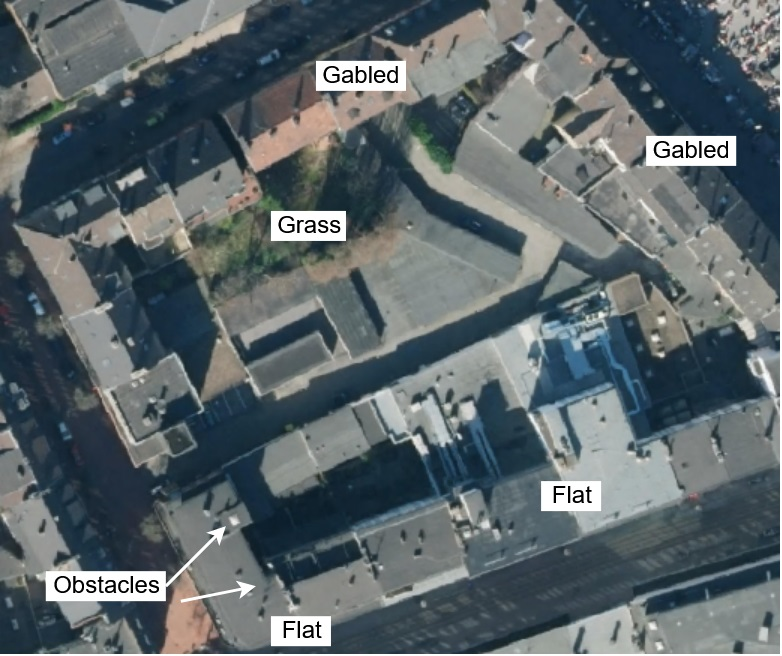
\includegraphics[clip, trim=0.0cm 0cm 0cm 0cm, width=0.55\linewidth]{chapter_5_mapping/imgs/challenge_urban-Page-2.jpg}
%     \caption{Satellite image of an urban environment with multiple flat roof landing sites. Select roof shapes and obstacles are labeled.}
%     \label{fig:ch1_challenge_urban}
% \end{figure}


\begin{figure}[t]
    \centering
  \begin{subfigure}{.45\linewidth}
    \centering
    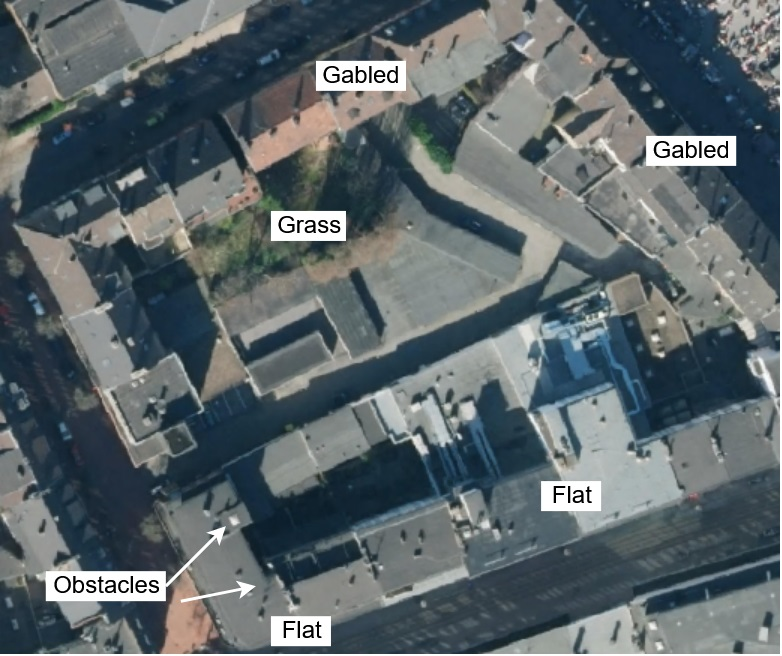
\includegraphics[clip, trim=0.0cm 0cm 0cm 0.55cm, width=0.95\linewidth]{chapter_5_mapping/imgs/challenge_urban-Page-2.jpg}
    \caption{}
    \label{fig:ch1_challenge_urban}
  \end{subfigure}
  \begin{subfigure}{.45\linewidth}
    \centering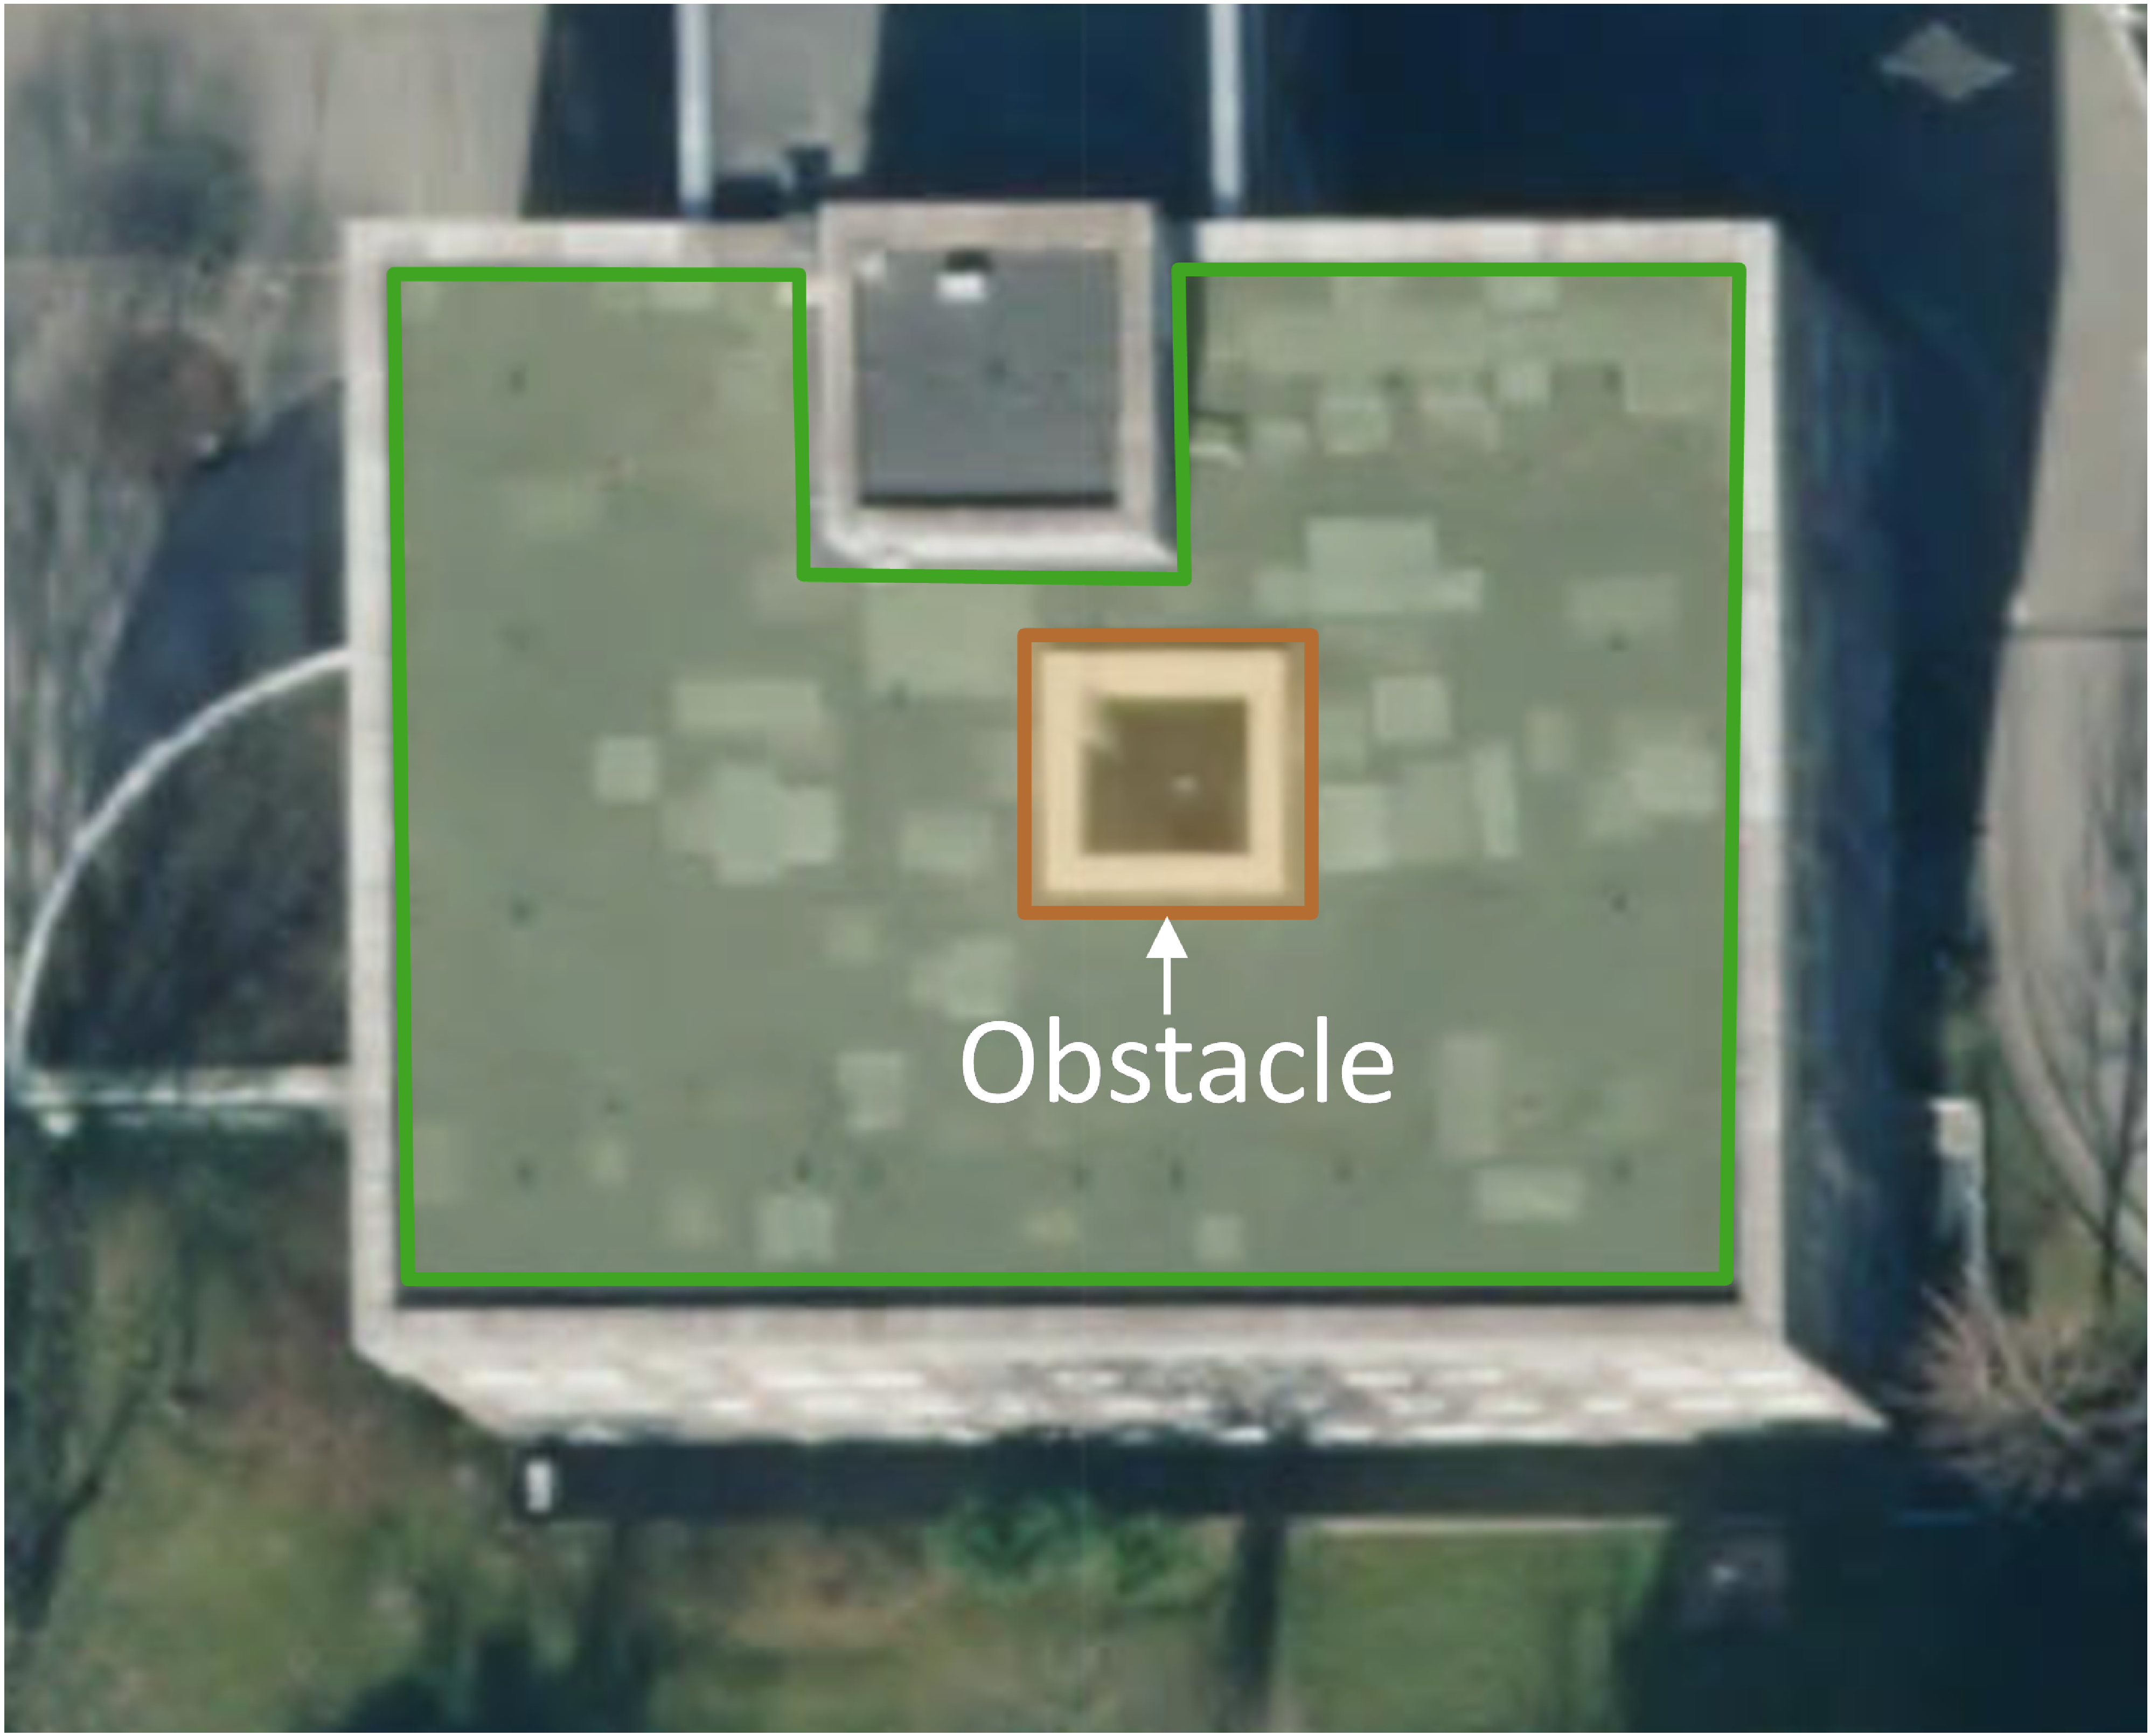
\includegraphics[width=.95\linewidth]{chapter_1_intro/imgs/roof_shape_obstacle.pdf}
    \caption{}
    \label{fig:ch1_roof_shape_obstacle}
  \end{subfigure}
  \caption[Motivation for rooftop landing]{(\subref{fig:ch1_challenge_urban}) Satellite image of an urban environment with multiple flat rooftops. Select roof shapes and obstacles are labeled.  (\subref{fig:ch1_roof_shape_obstacle}) A rooftop surface can be represented as a non-convex polygon with an exterior shell (green) and interior hole(s) (orange).  }\label{fig:ch1_motivation}
\end{figure}




\section{Problem Statement}

This dissertation aims to address the following challenges:

\begin{enumerate}[noitemsep]
    \itemsep0em 
    \item Where can a small UAS safely land in a city during an urgent or emergency landing situation?
    \item How can maps be constructed and risk evaluated for landing site selection and path planning?
    % \item What path should it take reach this landing site?
    \item How can the small UAS verify a landing zone is safe in real-time on approach to that site?
\end{enumerate}

Previous research has proposed the use of public Geographic Information Systems (GIS) datasets such as satellite images, airborne LiDAR point clouds, digital elevation maps, census data, and building outlines for terrain-based landing site identification, risk assessment, and path planning \cite{meuleau_emergency_2009, di_donato_evaluating_2017, patterson_timely_2014, bleier_risk_2015}.  However increased use of sUAS in urban cities motivates this work to additionally consider building rooftops as landing sites. To our knowledge this dissertation is the first work to explicitly use GIS data to automatically identify flat rooftop buildings, isolate flat surfaces, and find risk-minimum touchdown points that maximize distance to obstacles. 

% These conventional landing sites are often risk evaluated by terrain type and size \cite{di_donato_evaluating_2017}. 
\section{Research Approach and Thesis Outline}

% Map data is widely available in vector form, such as polygons, which describes features such as fields, parks, and building outlines \cite{openstreetmap_contributors_planet_2017}.  Such polygons can be efficiently stored and indexed such that spatial queries may efficiently computed in an embedded database \cite{furieri_spatialite_2017}. 

This dissertation proposes to process existing GIS data to extract safe landing sites and occupancy maps used for map-based planning. To accomplishing this several computational geometry algorithms have been developed to enable efficient extraction of flat surfaces as non-convex polygons. The overall structure of this dissertation is shown in Figure \ref{fig:ch1_thesis_overview} and can be summarized as accomplishing the following six tasks:
% This dissertation assumes these urgent landing scenarios are without loss-of-control, for example: low battery energy, lost communication link, adverse weather, non-essential sensor or actuator failure, operator emergency landing directive, and non-cooperative aircraft nearby.

\begin{enumerate}[noitemsep]
    \item Efficiently extract non-convex polygons with interior holes from 2D point sets. (Ch. 2)
    \item Extend polygon extraction methods from 2D point sets to 3D data where polygons represent flat surfaces and interior holes represent obstacles embedded on the surface. (Ch. 3)
    \item Classify rooftop shape in a city (e.g., flat) with high confidence in model prediction. (Ch. 4)
    \item Assimilate publicly available GIS data such as satellite images, airborne LiDAR point clouds, and existing map data into an urgent landing site database with associated risk metrics as well as occupancy maps for path planning. (Ch. 5)
    \item Create a multi-goal planner to efficiently search through candidate sites and account for landing site risk as well as flight path risk to that site. The planner identifies a landing site/path pair to minimize combined \emph{total} risk as well as computation time for this search. (Ch. 5)
    \item Perform experiments to verify the planned touchdown location is safe in real-time using on-board sensors such as LiDAR. (Ch. 6, Proposed)
\end{enumerate}

% The final risk-optimal landing site/path pair is sent to a navigation controller.
\begin{figure}[t]
    \centering
    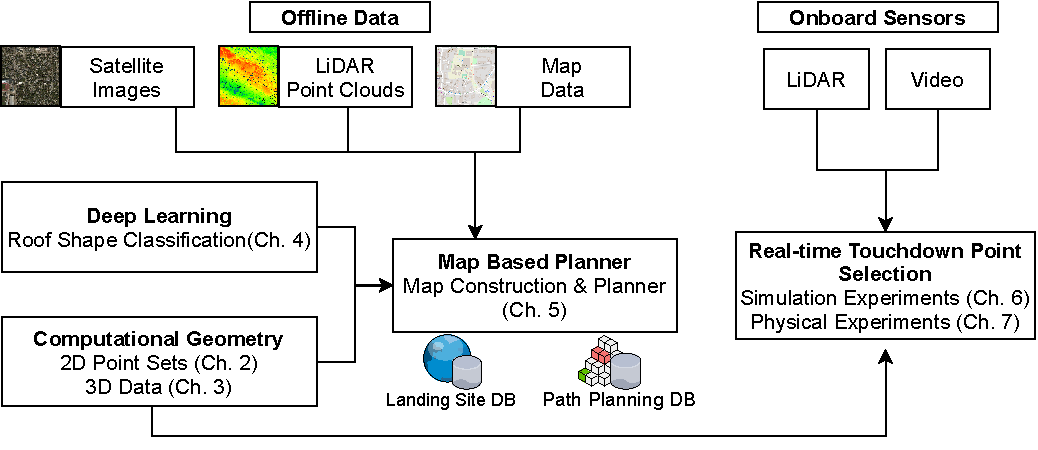
\includegraphics[width=0.70\linewidth]{chapter_1_intro/imgs/Challenge_Overview-thesis_overview.pdf}
    \caption{Overview of dissertation topics and structure.}
    \label{fig:ch1_thesis_overview}
\end{figure}

% \emph{How to efficiently construct databases from publicly available data to identify minimal-risk landing site for sUAS.}. Our previous stated observation of flat rooftop motivates 

% Numerous public datasets exist to aid construction of maps for aircraft urgent landing including satellite images, airborne LiDAR point clouds, census data, and existing building outlines. Our first goal is to efficiently transform this raw data into a risk evaluated landing site database which may be used for landing site selection and path planning.  Previous research has used such data to identity terrain based landing but none to our knowledge has focused on extracting flat rooftops \cite{atkins_emergency_2006, meuleau_emergency_2009, sankararaman_towards_2017, di_donato_evaluating_2017}. Our second goal is the construction of an efficient multi-goal planner which will account for both the intrinsic landing site risk as well as path risk. 



% Talk about data. Talk about the forms of data we have available for us to use: satellite images, airborne lidar points clouds, building outlines, census data. A host of information to help us make decision about places we can land.


\paragraph{Polygons from 2D Point Sets}

Characterizing the shape of a set of 2D points $\mathcal{P}$ has been a long-term focus of computational geometry research. A convex hull is defined as the smallest convex polygon that fully encapsulates all points in a set $\mathcal{P}$ as shown in Figure \ref{fig:ch1_convex_concave_1}.  Although widely used to estimate shape, point sets with non-convex distributions are poorly characterized by a convex hull \cite{duckham_efficient_2008}.  Convex hull over-estimation can be a serious issue when the points represent physical objects, e.g., obstacle free navigable areas. Several algorithms have been developed to construct shapes that ``fit'' or ``cover'' point sets more closely. These shapes are often termed non-convex polygons or concave hulls. 

The most notable examples of these algorithms are $\alpha$-shape \cite{edelsbrunner_shape_1983}, Spatialite concave hull \cite{furieri_spatialite_2017}, and PostGIS concave hull \cite{open_source_geospatial_foundation_postgis_2019}. Each is widely used in the computational geometry and GIS communities. These methods can extract the exterior boundary of a point set and also interior holes.  However, many of these methods are extremely slow motivating this dissertation to create an efficient non-convex (multi)polygon extraction algorithm called Polylidar. A key insight of this work is a novel boundary following method that contrasts computationally-expensive geometric unions of triangles. Real-world and synthetic benchmarks are presented to comparatively evaluate Polylidar speed and accuracy. Results show comparable accuracy and more than four times speedup compared to other open source concave polygon extraction methods. An example polygon from Polylidar is shown in Figure \ref{fig:ch1_convex_concave_2}.

% This dissertation uses the Open GeoSpatial Consortium (OGC) standard \cite{herring_opengis_2006-1} for defining \textit{linear ring} and \textit{polygon}. A linear ring is a consecutive list of points that is both closed and simple. This requires a linear ring to have non-intersecting line segments that join to form a closed path. The key components of a valid polygon are a single exterior linear ring representing the \emph{shell} of the polygon and a set of linear rings (possibly empty) representing \emph{holes} inside the polygon. 


\begin{figure}[t]

  \begin{subfigure}[t]{.22\linewidth}
    \centering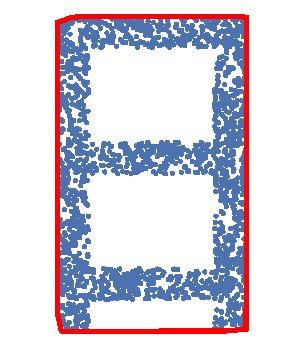
\includegraphics[width=.95\linewidth]{chapter_3_polylidar3d/imgs/concave_vs_convex_lettera_1.pdf}
    \caption{\label{fig:ch1_convex_concave_1}}
  \end{subfigure}
  \begin{subfigure}[t]{.22\linewidth}
    \centering
\includegraphics[width=.95\linewidth]{chapter_3_polylidar3d/imgs/concave_vs_convex_lettera_3.pdf}
    \caption{\label{fig:ch1_convex_concave_2}}
  \end{subfigure}
  \begin{subfigure}[t]{.26\linewidth}
    \centering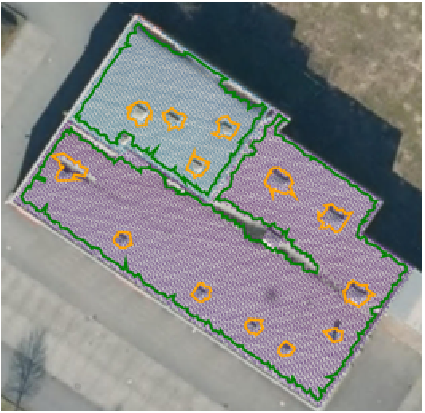
\includegraphics[width=.95\linewidth]{chapter_1_intro/imgs/rooftop_example_simple.pdf}
    \caption{\label{fig:ch1_rooftop_polygon}}
  \end{subfigure}
  \begin{subfigure}[t]{.26\linewidth}
    \centering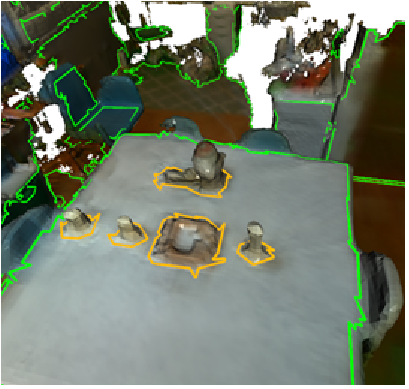
\includegraphics[width=.95\linewidth]{chapter_1_intro/imgs/mesh_example_simple.pdf}
    \caption{\label{fig:ch1_mesh_polygon}}
  \end{subfigure}
  \caption[Illustration of various polygons]{(a,b) Examples of a convex hull (red) and a non-convex polygon with holes from a 2D point set. (c,d) Examples of Polylidar3D's non-convex multi-polygon extraction from airborne LiDAR point clouds (colored by height) and a user provided mesh, respectively}\label{fig:ch1_polygon_examples}
\end{figure}


\paragraph{Polygons from 3D Data}

Flat surfaces are pervasive in engineered structures and also occur in natural terrain. For example, structures such as walls, floors, rooftops, and roadways are often flat or ``flat-like". 
% Similarly, home and office furnishings are typically composed of multiple flat surfaces.
Sensors such as LiDAR and RGBD cameras generate dense 3D point clouds of these predominately flat surface environments. This observation has been exploited for tasks in localization and mapping \cite{pathak_online_2010},  digital preservation with Photogrammetry and laser scanning \cite{malihi_3d_2016, lerma_terrestrial_2010, balsa-barreiro_generation_2018}, and point cloud registration \cite{rusinkiewicz_efficient_2001}. Planar segmentation techniques are often used to group points belonging to a common flat surface \cite{feng_fast_2014, pham_geometrically_2016-1, schaefer_maximum_2019}. However points clouds are dense incurring high computational cost when used directly in higher level tasks. Planar point clouds can be converted to lower dimensional representations such as polygons.
% Polygons reduce map size, accelerate matching for localization \cite{lee_indoor_2012-1}, and support model reconstruction and object detection \cite{cao_roof_2017}. 

Prior work has investigated transforming planar points clouds to convex polygons \cite{biswas_planar_2012,poppinga_fast_2008}.  Non-convex polygons can be generated using techniques such as $\alpha$-shapes but operate strictly on 2D data, requiring the projection of each 3D planar point cloud and expensive triangulation \cite{lee_fast_2013, edelsbrunner_shape_1983}. Pixel-level boundary following of organized point clouds (e.g., range images) can be used to extract non-convex polygons but often only captures the exterior shell of the polygon \cite{lee_indoor_2012-1}. These methods do not capture interior holes in a polygon needed to capture obstacles on flat surfaces. 

% Finally, many of the proposed solutions are limited in their use of 3D data, only working on range images and unable to handle unorganized forms of 3D data.

This dissertation introduces Polylidar3D, a non-convex polygon extraction algorithm that takes as input either unorganized 3D point clouds (e.g., airborne LiDAR point clouds), organized point clouds (e.g., range images), or user-provided meshes. A core idea of this work is to transform all data inputs into a half-edge triangular mesh for which planar segmentation and polygon extraction may occur in parallel. Dominant plane normals are identified and used to parallelize and regularize planar segments in the mesh. Triangles having similar normals to a dominant plane are grouped. Each group (in parallel) then performs region growing accounting for normal orientation, Euclidean distance, and point to plane distance. Immediately after a plane has been segmented a polygon extraction task is dynamically spawned. The result is a general and extremely fast framework for non-convex polygon extraction of 3D data. Polylidar3D is used in this dissertation to extract polygonal representations of flat rooftop surfaces and generated meshes as shown in Figure \ref{fig:ch1_polygon_examples}c,d.


% Speed is an important consideration for many of the applications mentioned previously. Parallel algorithms written for multi-core CPUs and GPUs should be used to reduce latency. 



\paragraph{Roof Shape Classification}



% Satellite images and 3D point cloud data from airborne LiDAR sensors provide complementary data on buildings. High resolution satellite images offer rich information content and are generally available worldwide.  However, extracting 3D building information from 2D images is difficult due to occlusion, poor contrast, shadows, and skewed image perspectives \cite{zhou_seamless_2014}. LiDAR point clouds provide depth and intensity measurements that capture the features of roof shapes, yet LiDAR does not offer other world feature information from ambient lighting intensity and color. LiDAR point cloud data are often processed and converted to digital surface models (DSM) representing the top surface layer of any terrain.

In an effort to identify suitable flat-like rooftops for urgent landing, our approach is to first predict the roof shapes of all buildings in cities by fusing satellite and LiDAR data with machine learning techniques. % Such classification will allow identification of rooftops suitable for landing, but also be generally beneficial for the \ac{GIS} community. % solar power panel placement, localization for UAS, 
Classical machine learning algorithms such as support vector machines (SVM), logistic regression, and decision trees are often used in these classification scenarios but invariably face computational complexity challenges caused by the high dimensionality found in GIS data sources.   To employ these algorithms, a reduction in dimensionality through feature selection is often performed. Prior work has performed roof classification through Support Vector Machine (SVM) and Random Forest classifiers by reducing a digital surface model (DSM) image of a roof to a set of handcrafted features \cite{mohajeri_city-scale_2018, assouline_building_2017}. Recent work has used Convolutional Neural Networks (CNN) to process satellite images and/or building DSMs to predict roof shape \cite{partovi_roof_2017, alidoost_knowledge_2016}.

This dissertation processes satellite images, airborne LiDAR point clouds, and city map  building outlines to generate both a LiDAR image and a cropped satellite image of each building. CNNs are independently trained for each modality to extract high level features for roof shape prediction. Features from both images are then fused to train a random forest classifier. This research contributes the first large multi-city annotated dataset of over 4,500 rooftops to train, validate, and test models.  Example annotated rooftops are shown in Figure \ref{fig:ch1_rooftop_shape_examples}. Several CNN models and classical machine learning algorithms are evaluated.

\begin{figure}[t]
\centering
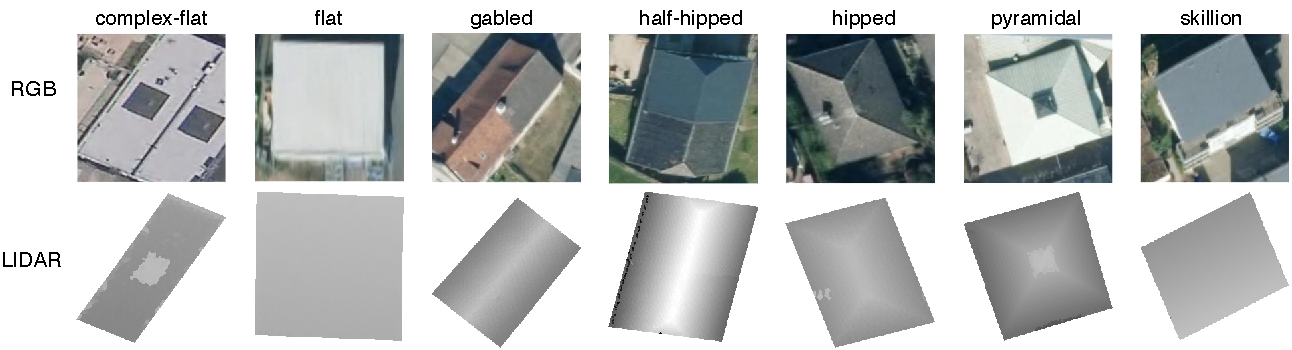
\includegraphics[width=0.99\textwidth]{chapter_4_roofshape/imgs/RoofShapes.pdf}
\caption[Satellite and LiDAR depth images of common rooftops]{Satellite (RGB) and LiDAR example images of roof shapes.}
\label{fig:ch1_rooftop_shape_examples}
\end{figure}


\paragraph{Map based Planner}


% Urban areas typically do not offer classic emergency landing sites such as unpopulated open fields. This requires a planner to consider unconventional yet safe alternatives.

% We propose flat building rooftops as viable urgent landing sites for small UAS. During landing site selection, a map-based planner must be able to assess \emph{landing site risk} posed to the aircraft and bystanders at touchdown. The UAS may pose risk to people and property it overflies enroute, so the planner must also assess \emph{path risk} once the landing flight plan is known.  Landing site and path risk together offer an estimate of \emph{total risk}.

Map data used for urgent landing planning must have high integrity and low-latency access to support timely decision making. This dissertation proposes an offline data processing pipeline and online multi-objective, multi-goal landing planner that enable a UAS to minimize total risk when a nearby landing is required. Landing site and local area map information is pre-processed and stored onboard.  Roof shape classifiers and Polylidar3D are both used to identify flat-like rooftops and extract landing surfaces as polygons. Geometric algorithms are used to process flat rooftop polygons to find the largest inscribed circle that maximizes distance to obstacles and defines optimal touchdown location on each flat roof.  A multi-goal real-time landing planner explores available ground and rooftop landing sites likely to minimize overall total risk while greedily pruning options known to have higher risk.  Pareto fronts over landing site and path risk are generated for three urban regions: Witten, Germany; Ann Arbor, Michigan; and mid-town Manhattan in New York City. We statistically analyze results with respect to availability and quality of landing sites as well as execution time of the map-based planner.

\paragraph{Landing Site Identification and Selection Experiments (In Progress and Proposed)}

A small UAS should utilize available sensors to verify a safe touchdown point upon approach to a landing site. We build upon our previous methods for offline landing site identification and selection to  use on-board sensors generating point clouds in real-time. Prior work has investigated converting these point clouds to 2D disparity grids \cite{desaraju_vision-based_2015} or probabilistic elevation maps \cite{forster_continuous_2015}. These methods then apply computer vision kernels over the grids to smooth and identify ``flat'' touchdown points. 
% Sensors such as LiDAR, RGBD cameras, or monocular cameras utilizing Structure from Motion (SfM) can generate 3D point clouds of the landing site. 
An alternative to operating over a discretized image space is modelling the 3D mesh of the roof. Polylidar3D can be used to rapidly construct a surface mesh and extract polygonal representations of all flat surfaces while accounting for obstacles. Afterward the largest inscribed circle in each polygon is defined. For the final dissertation,  flight experiments with small multicopter UAS carrying LiDAR sensors will be conducted to demonstrate and evaluate real-time map generation for landing site safety validation (in areas with small UAS landing site maps) or real-time landing identification and selection (in areas without small UAS landing site maps). Tests will be conducted in the M-Air netted flight facility where motion capture can provide ground truth data to be compared with UAS-generated landing site maps and decisions. 


\section{Contributions and Innovations}
% \vspace{1.5cm}
Specific contributions of this dissertation include: % things that have taken time / effort

\begin{itemize}[noitemsep]
  \item A faster open source library for non-convex (multi)polygon extraction from 2D point sets. An open source benchmark comparison of leading non-convex polygon extraction techniques in terms of accuracy and speed is provided. %\cite{Castagno_Github_Polylidar}.
%   \item An open source benchmark comparison of leading concave polygon extraction techniques from 2D point sets in terms of accuracy and speed.
  \item An efficient and versatile open source framework, Polylidar3D,  for non-convex (multi)polygon extraction from 3D data representing flat surfaces. Polylidar3D can handle unorganized and organized 3D point clouds as well as triangular meshes. Computation time is minimized with CPU multi-threading and GPU acceleration. %\cite{Castagno_Github_Polylidar}
  \item Multiple open source and reproducible experiments showing qualitative and quantitative benchmark results of Polylidar3D applied to sensors including LiDAR and RGBD cameras.
  \item A fast open source dominant plane normal estimation library, FastGA,  using a novel Gaussian Accumulator with efficient search.
  \item A deep learning framework for predicting roof shapes from a fusion of satellite image, airborne LiDAR point cloud, and existing building outline data. Over 4,500 buildings rooftops spanning three cities have been manually classified  for training, validation, and testing.
  \item A multi-goal planner that guarantees a risk-optimal solution is found rapidly by avoiding exploration of high-risk options. Plans are optimized over a combination of landing site and path risk metrics.
  \item (Proposed) Experimental UAS results of real-time landing site validation or identification/selection with Polylidar3D.
\end{itemize}
 
Specific innovations of this dissertation are: % things that have taken time / effort

\begin{itemize}[noitemsep]
      \item A novel computationally-efficient algorithm to extract non-convex polygons from 2D point sets while accounting for holes. The proposed method utilizes half-edge boundary following with edge-case detection instead of alternatives such as the expensive union of triangles.
      \item The first parallelized non-convex polygon extraction framework working with several forms of 3D data. Polygons represent dominant planar surfaces with interior holes representing the shape of obstacles embedded on their surface. Polylidar3D's speed and data input versatility allow its use for many applications.
    %   Triangle primitives are grouped according to dominant plane normals for which region growing occurs in parallel. Polygon extraction of segmented planar regions are spawned as dynamic tasks in a thread-pool. 
      \item The first large-scale multi-city analysis for predicting roof shapes. The provided annotated dataset contains diverse examples from small to large metropolitan city centers. 
      \item The first rigorous method to incorporate flat rooftops as candidate landing sites for urgent landing of small UAS in cities.  Optimal touchdown sites on rooftop surface are determined using geometric methods with risk evaluated according to size and proximity to alternative touchdown sites.
\end{itemize}


% Open Source C++ libraries (with Python bindings) are released at the following links:

% \begin{itemize}
%     \item Contribution 1 - {\small{ \url{https://github.com/JeremyBYU/polylidar/tree/polylidar2d}}}
%     \item Contribution 2 - {\small{ \url{https://github.com/JeremyBYU/polylidar}}}
%     \item Contribution 3 - {\small{\url{https://github.com/JeremyBYU/FastGaussianAccumulator}}}
%     \item Contribution 7 - TBD
% \end{itemize}

% Open Data sets are released at the following links:

% \begin{itemize}
%     \item Classified Roof Shape - {\small \url{https://www.mdpi.com/1424-8220/18/11/3960/s1}}
% \end{itemize}


\section{Products}

Publications, software, and datasets connected to this dissertation are:
\vspace{0.2cm}

\textbf{Conference}
\vspace{0.20cm}
\begin{itemize}[noitemsep]
    \item J. Castagno, C. Ochoa, and E. Atkins, ``Comprehensive Risk-based Planning for Small Unmanned Aircraft System Rooftop Landing,” in 2018 \emph{International Conference on Unmanned Aircraft Systems} (ICUAS), Jun. 2018, pp. 1031–1040, doi: 10.1109/ICUAS.2018.8453483.
    \item K. McDonough, J. Castagno, and J. Player, ``RANGR: Risk Aware Navigation and Gudiance Resilience,” presented at the \emph{AUVSI Xponential}, Denver, CO, USA, May 2018.
	\item J. Castagno and E. M. Atkins, ``Automatic Classification of Roof Shapes for Multicopter Emergency Landing Site Selection,” in 2018 \emph{Aviation Technology, Integration, and Operations Conference, American Institute of Aeronautics and Astronautics}, 2018.
\end{itemize}

\vspace{0.25cm}

\textbf{Journal}

\vspace{0.20cm}
\begin{itemize}[noitemsep]
    \item J. Castagno, M. Romano, P. Kuevor, and E. Atkins, ``Multi-UAV Wildire Boundary Estimation using a Semantic Segmentation Neural Network,” \emph{Journal of Aerospace Information Systems}. Sumbitted under review.
    \item J. Castagno and E. Atkins, ``Map-Based Planning for Small Unmanned Aircraft Rooftop Landing (In Press),” in \emph{Handbook on Reinforcement Learning and Control}, Springer, 2021. In Press.
    \item J. Castagno and E. Atkins, “Polylidar3D - Fast Polygon Extraction from 3D Data,” \emph{Sensors}, vol. 20, no. 17, Art. no. 17, Jan. 2020, doi: 10.3390/s20174819.
    \item J. Castagno and E. Atkins, “Polylidar - Polygons From Triangular Meshes,” \emph{IEEE Robotics and Automation Letters}, vol. 5, no. 3, pp. 4634–4641, Jul. 2020, doi: 10.1109/LRA.2020.3002212.
    \item J. Castagno and E. Atkins, “Roof Shape Classification from LiDAR and Satellite Image Data Fusion Using Supervised Learning,” \emph{Sensors}, vol. 18, no. 11, Art. no. 11, Nov. 2018, doi: 10.3390/s18113960.
\end{itemize}

\textbf{Open Source C++ libraries (with Python bindings)}

\begin{itemize}[noitemsep]
    \item J. Castagno, ``Polylidar3D,''   [Online]  Available: \url{https://github.com/JeremyBYU/polylidar}, 2020.
    \item J. Castagno, ``Fast Gaussian Accumulator,''   [Online]  Available: \url{https://github.com/JeremyBYU/FastGaussianAccumulator}, 2020.
    \item J. Castagno, ``Organized Point Filters,''   [Online]  Available: \url{https://github.com/JeremyBYU/OrganizedPointFilters}, 2020.
\end{itemize}

\textbf{Open Data Sets}

\begin{itemize}[noitemsep]
    \item J. Castagno, ``Annotated Roof Shape Dataset,''   [Online]  Available: \url{https://www.mdpi.com/1424-8220/18/11/3960/s1}, 2018.
\end{itemize}


 
\chapter{Polygons from 2D Point Sets}
 \label{ch:polylidar}
 \section{Introduction}

% Talk about need for 2D point set to convex polygons. Connection to multiple fields!

This chapter presents Polylidar, an efficient algorithm to transform 2D point sets into simplified non-convex (i.e., concave) polygons with holes. Polylidar begins by triangulating the point set and filtering triangles given user-specified parameters such as maximum triangle edge length. Once filtering is complete, edge-connected triangles are combined into regions creating a set of triangular meshes representing the shape of the point set. Next, Polylidar converts each mesh region to a polygon through a novel boundary following method which accounts for holes. Figure \ref{fig:ch2_convex_concave}b shows Polylidar applied to a 2D point set while (c) shows Polylidar used on a plane segmented point cloud from an RGBD image.


\begin{figure}[t]
    \centering
  \begin{subfigure}{.25\linewidth}
    \centering
    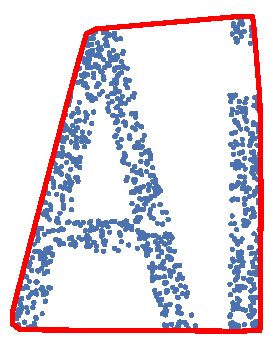
\includegraphics[clip, trim=0.0cm 0.1cm 0.0cm 0.25cm, width=0.99\linewidth]{chapter_2_polylidar/imgs/concave_vs_convex_0.pdf}
    \caption{}
    \label{fig:ch2_convex}
  \end{subfigure}
  \begin{subfigure}{.25\linewidth}
    \centering
    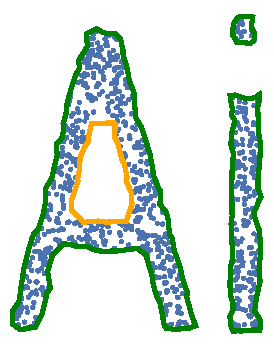
\includegraphics[clip, trim=0.0cm 0.1cm 0.0cm 0.25cm, width=.99\linewidth]{chapter_2_polylidar/imgs/concave_vs_convex_2.pdf}
    \caption{}
    \label{fig:ch2_concave}
  \end{subfigure}
  \begin{subfigure}{.25\linewidth}
    \centering
    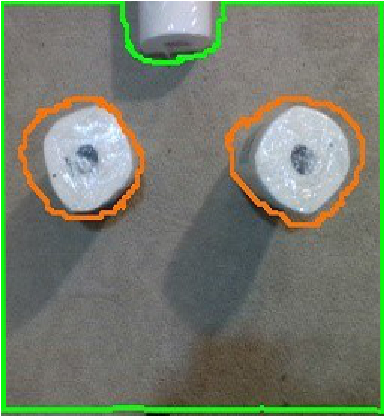
\includegraphics[width=0.99\linewidth]{chapter_2_polylidar/imgs/RealSensePictures-cropped_aspect.pdf}
    \caption{}
    \label{fig:ch2_realsense}
  \end{subfigure}
  \caption[Demonstration of Polylidar]{(a) Convex hull of a point set (red); (b) MultiPolygon extraction using Polylidar (green).
  (c) Polygon extraction from a plane segmented point cloud from an Intel RealSense RGBD camera capturing paper towel rolls on a basement floor. 
  Note that Polylidar also identifies holes (orange).}
  \label{fig:ch2_convex_concave} 
\end{figure}



We show that the Polylidar algorithm is approximately 4 times faster than leading open source approaches for concave polygon extraction. Polylidar's speed is attributed to rapidly identifying boundary edges (shell and holes) and then performing  boundary following to ensure a valid polygon is returned. 


Contributions of this chapter are:
\begin{itemize}
  \item A faster open source \cite{Castagno_Github_Polylidar} concave (multi)polygon extraction algorithm from 2D point sets.
  \item A benchmark comparison of leading concave polygon extraction techniques in terms of accuracy and speed.
%   \item Real-world validation of Polylidar on 3D point data.
\end{itemize}
% Please refer to \cite{DBLP:journals/corr/abs-1903-03829} for Polylidars technique for planar mesh extraction from 3D points.

Below, Sections \ref{sec:ch2_background} and \ref{sec:ch2_prelim} provide background on non-convex shape generation and mathematical preliminaries, respectively. Section \ref{sec:ch2_methods} describes Polylidar algorithms, while Section \ref{sec:ch2_results} shows benchmark test results of Polylidar versus other methods.  Section \ref{sec:ch2_random_polygons_test} describes test results. Sections  \ref{sec:ch2_discussion} and \ref{sec:ch2_conclusion} provide discussion and conclusions.



\section{Background}\label{sec:ch2_background}

Characterizing the shape of a set of 2D points $\mathcal{P}$ has been a long-term focus of computational geometry research. A convex hull is defined as the smallest convex polygon that fully encapsulates all points in a set $\mathcal{P}$.  Although widely used to estimate shape, point sets with non-convex distributions are poorly characterized by a convex hull \cite{duckham_efficient_2008}.  Convex hull over-estimation can be a serious issue when the points represent physical objects, e.g., obstacle free navigable areas. Several algorithms have been developed to construct shapes that ``fit'' or ``cover'' point sets more closely. 

Figure \ref{fig:ch2_convex_concave} compares convex and concave hulls. Figure \ref{fig:ch2_convex_concave}b is the multipolygon output of Polylidar described below.
%One may argue that the red convex hull does not conform well to the point distribution but the green concave hull captures the shape of the letters more precisely. 
While there is a unique convex hull, there is no true or unique concave hull.  Concave hull algorithm implementations can also have different output types.  Some return only an unordered set of edges while others return a single polygon.  Some algorithms return multiple disconnected polygons (multipolygon), and some can generate holes inside a polygon.

The $\alpha$-shape algorithm is an early strategy to generate a family of shapes ranging from a convex hull to a point set  \cite{edelsbrunner_shape_1983}. The parameter $\alpha$ dictates the radius of a closed disk used to prune/remove area in the convex hull. This disk is allowed to move freely shaving off the excess shape until it finds points. When disk radius is large, ideally infinite, the convex hull is produced; when disk radius is infinitesimally small only the points remain. A common implementation of $\alpha$-shape organizes points using Delaunay triangulation and filters triangles whose circumcircle radius is less than $\alpha$.  The final shape is represented by the remaining edges and triangles.  Note that the $\alpha$-shape method creates multiple non-intersecting shapes with the possibility of holes. 

The algorithm in \cite{duckham_efficient_2008} produces polygons from point sets called $\chi$-shapes. Like some $\alpha$-shape implementations, the $\chi$-shape approach begins with Delaunay triangulation to order and spatially connect data points.  The algorithm differs by iteratively removing the longest exterior edges from triangulation based on a specified maximum length parameter $l$. A corner case occurs  when edge removal results in a non-simple polygon, i.e., the polygon wraps into itself; in this case edge removal is skipped.  The $\chi$-shape produced is a single polygon with no possibility of holes.

The geospatial software library Spatialite \cite{furieri_spatialite_2017}, an extension to SQLite \cite{hipp_sqlite_2020}, contains a concave hull extraction procedure. The algorithm again starts with Delaunay triangulation then analyzes the distribution of each triangle's edge length to determine mean $\mu_l$ and standard deviation $\sigma_l$. Any triangle with edge length greater than $C \cdot \sigma_l  + \mu_l$ is removed, where $C$ is a user-defined parameter. The final geometry returned is the union of all triangles computed with GEOS, a high performance open source geometry engine. The output may be a multipolygon (i.e., multiple disjoint polygons) with the possibility of holes inside each. 

PostGIS is a geospatial database of computational geometry routines such as the concave hull method in \cite{open_source_geospatial_foundation_postgis_2019}. This algorithm first calculates the convex hull and then shrinks the hull by adjusting vertex connections to closer points which ``cave in'' the hull.  This process recursively shrinks a boundary until a user-specified percent reduction in area from the convex hull is achieved. The resulting shape is a single polygon with the possibility of holes. 

\begin{table}[ht]
\centering
\caption{Concave Hull Extraction Methods}
\label{table:ch2_compare_alg}
\begin{tabular}{ccc}
\hline
Algorithm                                                   & Output                                                           & Holes? \\ \hline
$\chi$-shapes                                             & \begin{tabular}[c]{@{}c@{}}unordered\\ set of edges\end{tabular} & No     \\
\begin{tabular}[c]{@{}c@{}}CGAL $\alpha$-shape\end{tabular}   & \begin{tabular}[c]{@{}c@{}}unordered\\ set of edges\end{tabular} & Yes    \\
Spatialite                                                 & (multi)polygon                                                   & Yes    \\
PostGIS                                                       & polygon                                                          & Yes    \\
Polylidar (new)                                                   & (multi)polygon                                                   & Yes    \\ \hline
\end{tabular}
\end{table}

Table \ref{table:ch2_compare_alg} provides a summary  of the concave hull algorithms discussed above. The Computational Geometry Algorithms Library (CGAL) is  used as the implementation of the $\alpha$-shape method \cite{the_cgal_project_cgal_2019}. Note that the time complexity of all algorithm implementations, with the exception of PostGIS, is $\mathcal{O}(n\log{}n)$.  This chapter contributes a procedure to more rapidly compute (multi)polygon output with the possibility of holes.  Though this is a complex output to generate, we show through benchmarks that our algorithm and implementation outperforms other available approaches.

\section{Preliminaries}\label{sec:ch2_prelim}

A 2D \textit{point set} is an arbitrarily ordered set of two dimensional points in a Cartesian reference frame. Each point is defined by orthogonal bases $\hat{\mathbf{e}}_x$ and $\hat{\mathbf{e}}_y$  with
\begin{equation}
\label{eq:ch2_point}
    \vec{{p}_{i}}=x\,\hat{\mathbf{e}}_x+y\, \hat{\mathbf{e}}_y= [x,y]
\end{equation}
where $x,y$ are plane coordinates.

An $n$-point array $\mathcal{P} = \{ \vec{{p}_{1}}, \vec{{p}_{i}}, \ldots, \vec{{p}_{n}} \}$ contains points $\vec{{p}_{i}} \in \mathbb{R}^2$ indexed by $i$.  A triangular mesh $ \mathcal{T}$ is defined by
\begin{equation}
\label{eq:ch2_tri}
    \mathcal{T} = \{ t_1, t_i, \ldots, t_{k} \}
\end{equation}
where each $t_i$ is a triangle with vertices defined by three point indices $\{i_1, i_2, i_3\} \in \left[1,n\right]$ referencing points in $\mathcal{P}$.

We follow the Open Geospatial Consortium (OGC) standard \cite{herring_opengis_2006-1} for defining \textit{linear ring} and \textit{polygon}. A linear ring is a consecutive list of points that is both closed and simple. This requires a linear ring to have non-intersecting line segments that join to form a closed path. The key components of a valid polygon are a single exterior linear ring representing the \emph{shell} of the polygon and a set of linear rings (possibly empty) representing \emph{holes} inside the polygon. 

\section{Methods}\label{sec:ch2_methods}

% Polylidar generates 2D concave polygons from 2D or 3D point set inputs. The only difference between handling 3D and 2D point sets is additional triangle filtering based upon user specified planarity constraints. 
Sections \ref{sec:ch2_tri}, \ref{sec:ch2_triangle_filtering_2d}, and \ref{sec:ch2_mesh_extraction} describe the triangulation data structures, filtering, and mesh extraction respectively.  Section \ref{sec:ch2_polygon_extraction} describes polygon extraction. %while Section \ref{sec:time_complexity} describes time complexity.
\subsection{Triangulation with Half-Edge Decomposition} \label{sec:ch2_tri}

Polylidar begins with the Delaunator library \cite{noauthor_github_2018} performing a Delaunay triangulation of point set $\mathcal{P}$. The original algorithm was written in JavaScript but a C++ port of the library is used in Polylidar \cite{noauthor_github_2018-1}. Note that we have modified Delaunator to use robust geometric predicates to ensure correctness during triangulation \cite{richard_shewchuk_adaptive_1997}. Delaunator was chosen for its ease of integration, speed, and output data structure which returns a \emph{half-edge} triangulation. A half-edge triangulation decomposes a shared edge using two half-edges A$\rightarrow$B and B$\rightarrow$A. An example of this decomposition and resulting data structures is shown in Figure \ref{fig:ch2_delaunator}. 


% In a triangulation a triangle's edge is often shared with another triangle (except the outer edges which form the convex hull); a half-edge refers to one side of this shared edge. 
% Some triangulation implementations refer to a shared edge as A$\leftrightarrow$B while Delaunator


\begin{figure}[ht]
    \centering
  \begin{subfigure}{.25\linewidth}
    \centering
    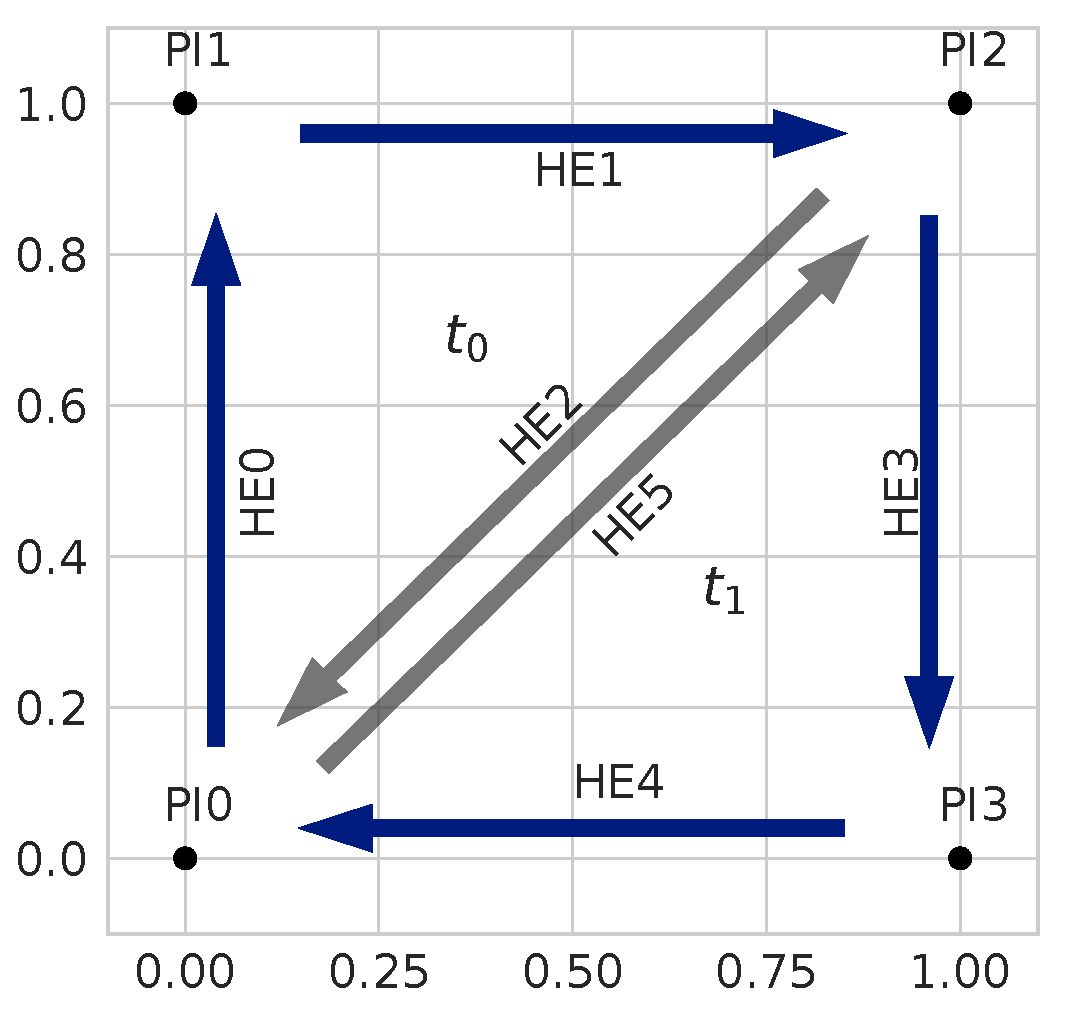
\includegraphics[width=0.99\linewidth]{chapter_2_polylidar/imgs/delaunator_tri-min.pdf}
    \caption{}
    \label{fig:ch2_delaunator_tri}
  \end{subfigure}
  \begin{subfigure}{.25\linewidth}
    \centering
    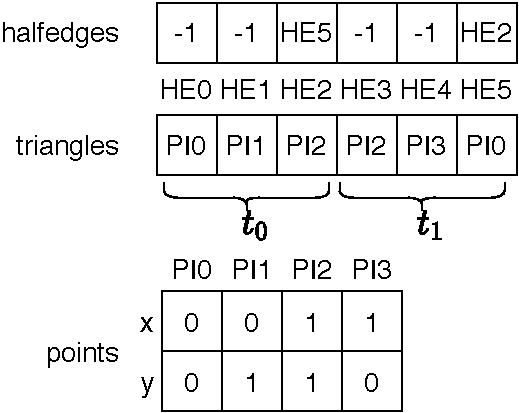
\includegraphics[width=.99\linewidth]{chapter_2_polylidar/imgs/DelaunatorDS.pdf}
    \caption{}
    \label{fig:ch2_delaunator_ds}
  \end{subfigure}
  \caption[Delaunay triangulation example]{(a) Triangulation of a square point set using Delaunator \cite{noauthor_github_2018} with output data structure indexed by half-edge ids in (b).  HE=half-edge, PI=point index, $t$=triangle. Grey edges show shared edges decomposed individually.}
  \label{fig:ch2_delaunator} 
\end{figure}


Figure \ref{fig:ch2_delaunator}a triangulates point set $\{\text{PI0, PI1, PI2, PI3}\}$.  Triangulation produces two triangles, $t_0$ and $t_1$, with half-edges $\{\text{HE0, HE1, HE2}\}$ and $\{\text{HE3, HE4, HE5} \}$, respectively.  Each half-edge supports clockwise travel to the next half-edge in that triangle's edge set. Figure \ref{fig:ch2_delaunator}b lists the resulting $halfedges$, $triangles$, and $points$ data structures.  The $halfedges$ array is indexed by a half-edge reference id. It provides the opposite half-edge of a shared edge if it exists; otherwise -1 is returned. The $triangles$ array is also indexed by half-edge id and gives the starting point index of the associated half edge. The relationship between half-edge and triangle indices is $t = \operatorname{floor}(he / 3)$.

\subsection{Triangle Filtering}\label{sec:ch2_triangle_filtering_2d}
As with Spatialite and $\alpha$-shape methods the initial shape starts with $k$ triangles in $\mathcal{T}$ per Eqn. \ref{eq:ch2_tri} returned from Delaunay triangulation. Also similar to $\alpha$-shape and Spatialite methods, Polylidar filters triangles by configurable criteria for each triangle. Polylidar allows the user to perform triangle filtering using either the $\alpha$ parameter or maximum triangle edge length parameter $l_{max}$. The filtered triangle set is denoted $\mathcal{T}_f$. 



\subsection{Triangular Mesh Region Extraction}\label{sec:ch2_mesh_extraction}

An iterative plane extraction procedure inspired from \cite{cao_roof_2017} generates subsets of $\mathcal{T}_f$ that are spatially connected.  These subsets are denoted  $\mathcal{T}_r$ which represent triangular mesh \emph{regions}. A spatial connection between triangles exists when they share an edge. A random seed triangle is selected from $\mathcal{T}_f$ where a new region is created and expanded by its adjacent edge neighbors from the \emph{halfedges} data structure. Region growth halts when no more triangles in $\mathcal{T}_f$ connect to the region. The process repeats with another seed triangle until all triangles in $\mathcal{T}_f$ have been examined. 


\begin{figure}[ht]
    \centering
  \begin{subfigure}{.3\linewidth}
    \centering
    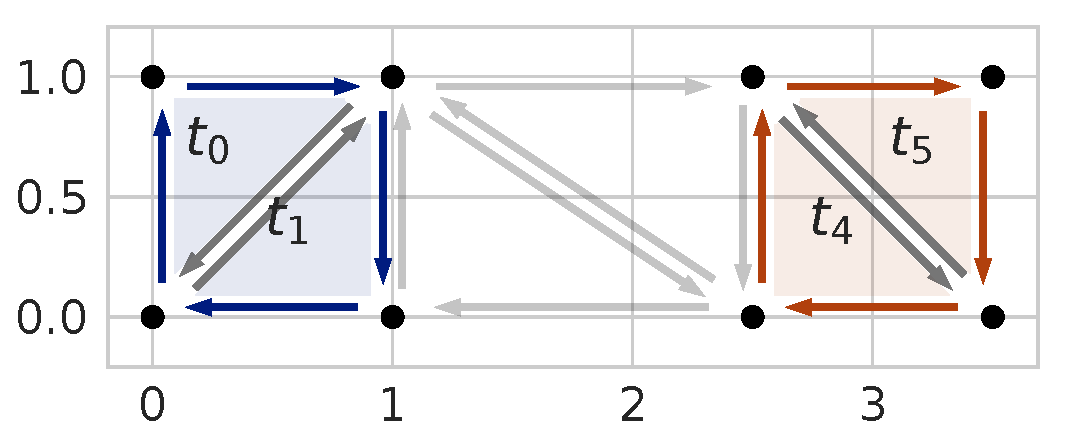
\includegraphics[width=0.99\linewidth]{chapter_2_polylidar/imgs/plane_extraction_a-min.pdf}
    \caption{}
    \label{fig:ch2_plane_extraction_a}
  \end{subfigure}
  \begin{subfigure}{.3\linewidth}
    \centering
    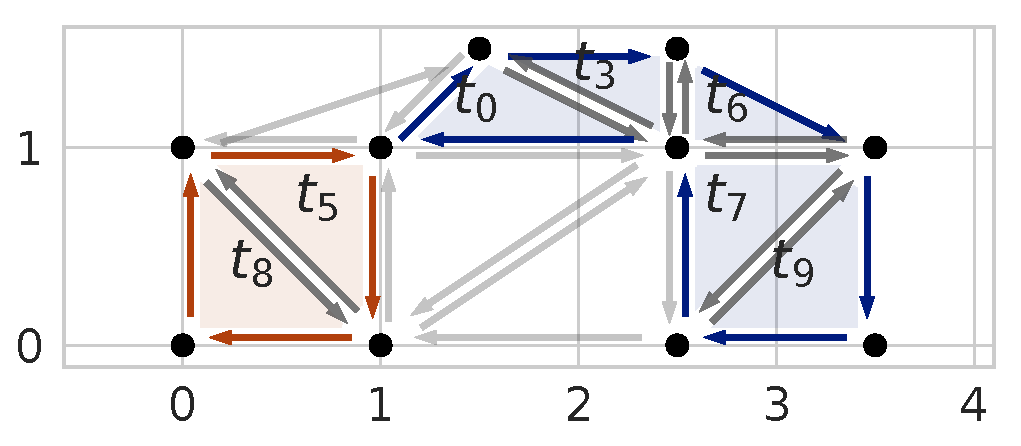
\includegraphics[width=.99\linewidth]{chapter_2_polylidar/imgs/plane_extraction_b-min.pdf}
    \caption{}
    \label{fig:ch2_plane_extraction_b}
  \end{subfigure}
  \caption[Region growing example from triangulation]{(a) Example of two regions extracted denoted by orange and blue. Triangles $t_0$ and $t_1$ are one region while $t_4$ and $t_5$ are another. (b) Two regions are also extracted with a shared vertex.}
  \label{fig:ch2_plane_extraction} 
\end{figure}


 Figure \ref{fig:ch2_plane_extraction}a shows triangular mesh region examples. Distinct regions are shown in orange and blue; light grey edges denote triangles that have been filtered out.  
 %  If you don't describe algorithmically or mathematically how (b) happens cleverly, then don't highlight it in the text!  --> Figure \ref{fig:plane_extraction}b shows that blue and orange regions are not spatially connected by a single vertex (1,1). 
 The output of this step is a set of spatially connected triangular mesh regions, $\mathcal{T}_R$, where each specific region, $\mathcal{T}_{r,i}$, is a set of triangle \emph{indices}. We denote the set of $m$ triangular mesh regions as:

\begin{align}
    \mathcal{T}_R = \{ \mathcal{T}_{r,1}, \mathcal{T}_{r,i},  \ldots, \mathcal{T}_{r,m} \} \\
    \mathcal{T}_{r,i} =  \{ t_{i}, \ldots, t_{j} \}
\end{align}


\subsection{2D Polygon Extraction}\label{sec:ch2_polygon_extraction}

Polygon extraction has three steps: data structure initialization, concave shell extraction, and hole(s) extraction. Each of these steps is described below. Note that polygon extraction is independent of the specific triangular mesh regions $\mathcal{T}_{r,i}$, thus subsequent notation will drop the $i$ index for brevity when used in algorithms. The following steps are executed for each of the $m$ regions in $\mathcal{T}_{R}$ to generate $m$ polygons.

\subsubsection{Data structure initialization}

Data structure initialization is shown in Algorithm \ref{alg:ch2_boundary_edges} which produces three data structures: a boundary half-edge set, a point index hash map, and the extreme point. A visual example of these data structures is shown in Figure \ref{fig:ch2_algorithm1_visual}. Boundary half-edge set $\mathcal{BE}$ contains the half-edge indices that are on the exterior border of a region, marked in blue in Figure \ref{fig:ch2_algorithm1_visual}a.  A half-edge is marked as a boundary if it has no opposite half-edge (meaning it is on the convex hull of the full triangulated set) or if its adjacent triangle is not in $\mathcal{T}_{r,i}$. The last check is important because a half-edge may share an edge with an interior triangle that is not part of $\mathcal{T}_{r,i}$ as seen in the rightmost edge for the blue region in Figure \ref{fig:ch2_plane_extraction}a. The \emph{halfedges} data structure is fixed at triangulation and is not aware of filtered triangles or the regions discussed in Section \ref{sec:ch2_mesh_extraction}.

\begin{figure}[ht]
    \centering
  \begin{subfigure}[t]{.30\linewidth}
    \centering
    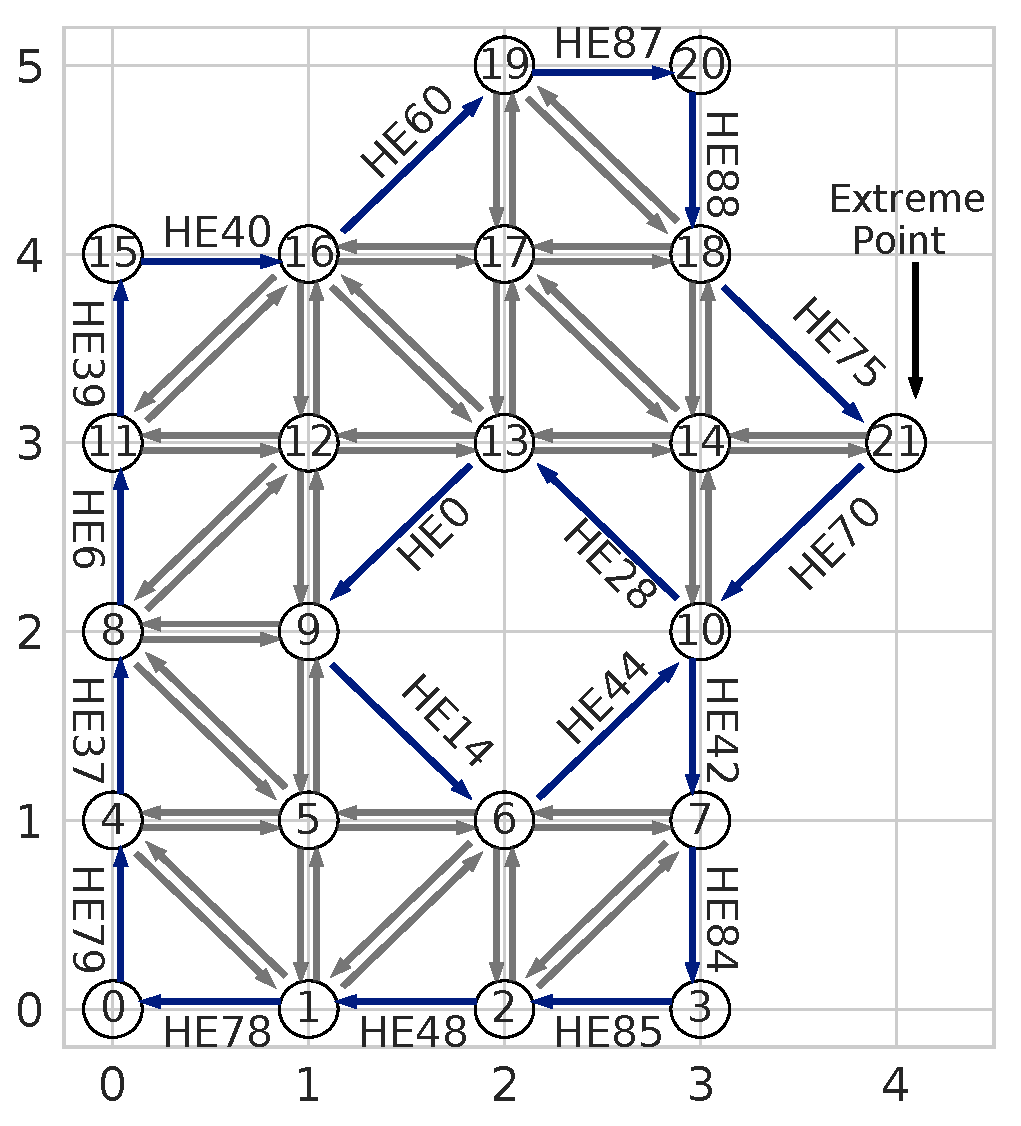
\includegraphics[width=0.99\linewidth]{chapter_2_polylidar/imgs/algorithm1_visual.pdf}
    \caption{}
    \label{fig:ch2_algorithm1_visual_boundary}
  \end{subfigure}
  \begin{subfigure}[t]{.25\linewidth}
    \centering
    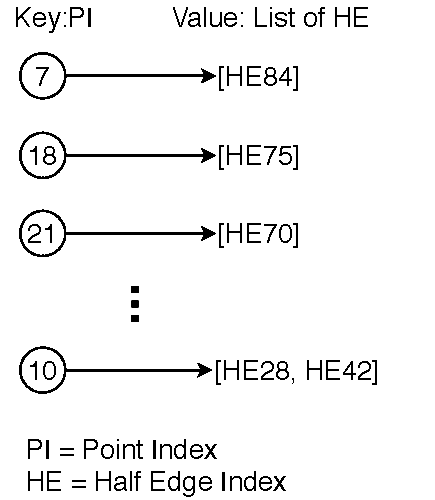
\includegraphics[clip, trim=0cm 0cm 0.5cm 0cm,width=.99\linewidth]{chapter_2_polylidar/imgs/HashMap_PS.pdf}
    \caption{}
    \label{fig:ch2_hashmap}
  \end{subfigure}
  \caption[Representation of boundary half-edge set, extreme point, and point index hash map]{(a) The boundary half-edge set is marked in blue and point index 21 (PI21), the farthest point on the x-axis, is noted. (b) A sample of the resulting point index hash map, $PtE$ is shown. Note that the display order has been arbitrarily chosen.  }
  \label{fig:ch2_algorithm1_visual} 
\end{figure}

The second data structure is a point index hash map, $PtE$, whose \emph{key} is a point index and \emph{value} is a \emph{list} of outgoing boundary half-edges from the keyed point index. This \emph{unordered} hash map is represented in Figure \ref{fig:ch2_algorithm1_visual}b; note the keyed point index 7 mapping to the single element list containing half-edge 84. The final data structure represents an extreme point in the triangle mesh, referring to the point farthest to the right on the $x$-axis. This point will be used as the starting point index when extracting the concave hull to help ensure extraction does not start on a hole edge. Multiple points may exist on the extreme edge;  the algorithm will track the first one found in this case. 

\begin{algorithm}[ht]
    \SetKwInOut{Input}{Input}
    \SetKwInOut{Output}{Output}

    \Input{Triangular Mesh Region , $\mathcal{T}_r = \{t_i, \ldots, t_k\}$ \\
        Shared Halfedges, $halfedges$ \\
        Triangles Point Index, $triangles$ 
    }
    
    \Output{Half Edge Set , $\mathcal{BE} = \{he_i, \ldots, he_n\}$ \\ 
        Point Index Hash Map, $PtE$ \\

        Extreme Point, $pi_{xp}$ } 
    $\mathcal{BE} = \emptyset$ \tcp*{boundary half-edge set}
    $PtE = \emptyset$ \tcp*{Point to half-edge hashmap}
    $pi_{xp} = 0$ \tcp*{will be overwritten}
    \For{$t_i \in \mathcal{T}_r$} { 
        \For{$he_i \in t_i$} { 
            $he_j = halfedges[he_i]$\tcp*{opposite edge}
            $t_j = \operatorname{floor}(he_j / 3)$ \tcp*{adjacent tri}
            \uIf{$t_j \notin \mathcal{T}_r$}{
                $\mathcal{BE}$ = $\mathcal{BE}$ + $he_i$ \tcp*{boundary edge} 
                $pi = triangles[he_i]$ \\
                $pi_{xp} = \operatorname{TrackXp}(pi, pi_{xp})$ \\
                \uIf{$pi \notin PtE$}{
                    \tcc{create half-edge list}
                    $PtE[pi] = [he_i]$ 
                    % \tcc{Add new half edge list}
                }
                \uElse {
                    $\operatorname{Append}(PtE[pi], he_i)$
                }
            }
        }
  
    }
    return $\mathcal{BE}, PtE, pi_{xp}$
    \caption{Initialize Data Structures for Polylidar}\label{alg:ch2_boundary_edges}
\end{algorithm}


\subsubsection{Concave Shell Extraction}
Outer shell extraction begins by traversing the half-edge graph, starting with the half-edge provided by the extreme point. As the edges are traversed the point indices are recorded in a list representing the linear ring of the concave hull. Edges are removed from the boundary half-edge set, $\mathcal{BE}$, as they are traversed.  In Figure \ref{fig:ch2_algorithm1_visual}a the extreme point index is PI21 and the starting half-edge is HE70. This starting half edge and start point index are arguments to the \texttt{ExtractLinearRing} procedure in Algorithm \ref{alg:ch2_concave_hull_shell}, with the procedure halting when edge traversal returns back to the starting point index, indicating a closed linear ring has been extracted. The hole in this shape, represented by edges (HE28, HE0, HE14, HE44), with a shared vertex at PI10, must be carefully handled as explained below. This is an example of an non-manifold mesh.

The example in Figure \ref{fig:ch2_algorithm1_visual} begins with HE70 traversing to PI10. The outgoing boundary half-edges for this point index are determined from $PtE$ which provides a list of both HE28 and HE42. However HE28 is an edge for a hole in this polygon while HE42 is the correct half-edge to traverse for the outer shell. The \texttt{SelectEdge} procedure determines which of these edges to choose and is visually outlined in Figure \ref{fig:ch2_example1}a. Angles between the proposed edges and previous edge HE70 are calculated and the edge with the largest angle is chosen which guarantees the largest concave hull.  This edge cannot be a hole edge because that would imply that the hole is outside the concave shell, which is invalid.

% {\color{blue}
On rare occasions the extreme point may have more than one outgoing half edge, meaning that a hole is connected to it.  This can be handled in the same way stated above by using the \texttt{SelectEdge} procedure. The only difference is that the previous hull edge is not known (the procedure has just started), but since we know we are on the far right of the hull we can substitute the previous edge for the unit vector [0,1] per Figure \ref{fig:ch2_example1}b. This unit vector is guaranteed to provide a stable order of the angle differences which would have been provided by the actual previous hull edge.

\begin{algorithm}
    \SetKwInOut{Input}{Input}
    \SetKwInOut{Output}{Output}

    \Input{Half Edge Set , $\mathcal{BE} = \{he_i, \ldots, he_n\}$ \\ 
            Point Index Hash Map, $PtE$ \\
            Starting half-edge, $he$ \\
            Start point index, $startPI$ \\
            Triangles Point Index, $triangles$
    }
    \Output{Linear Ring , $lr = [pi_1, \ldots, pi_k]$ } 
    $lr = [\;]$  \tcc*{empty linear ring}
    \While{True}{
        $\mathcal{BE} = \mathcal{BE} \setminus he $ \\
        $he_t = \operatorname{NextTriangleEdge}(he)$\\
        $pi = triangles[he_t]$ \\
        $\operatorname{Append}(lr, pi)$\\
        \uIf{$pi \; is \; startPI$}{
            \tcc{closed linear ring}
            break
            % \tcc{Add new half edge list}
        }
        $nextEdges = PtE[pi]$ \\
        $he = \operatorname{SelectEdge}(he, nextEdges)$
    }
    return $lr$
    \caption[Extract Linear Ring]{ExtractLinearRing}\label{alg:ch2_concave_hull_shell}
\end{algorithm}



% \begin{figure}[ht]
%     \centering
%   \begin{subfigure}[t]{.35\linewidth}
%     \centering
%     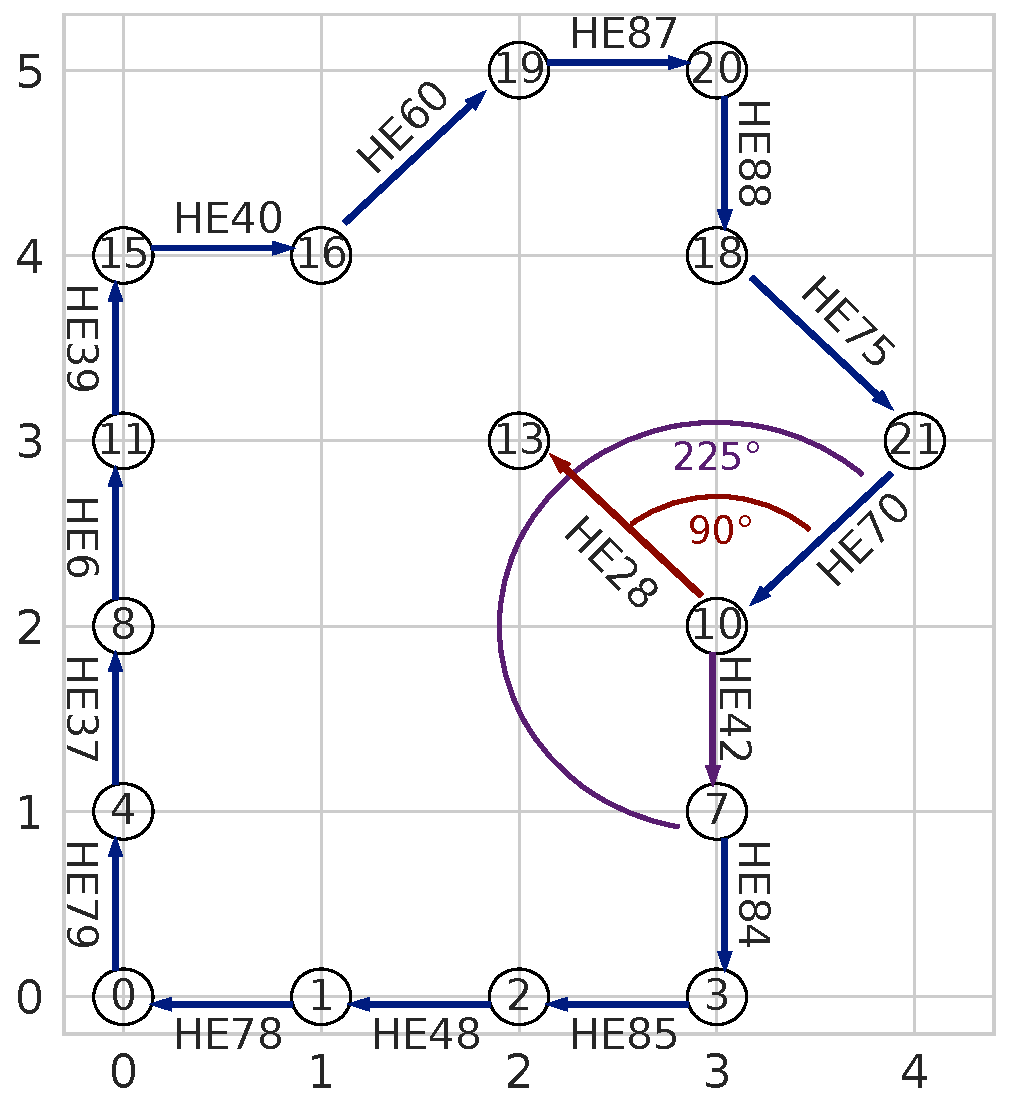
\includegraphics[width=0.99\linewidth]{chapter_2_polylidar/imgs/example_one_hole_choice_visual.pdf}
%     \caption{}
%     \label{fig:ch2_example1_non_extreme}
%   \end{subfigure}
%   \begin{subfigure}[t]{.35\linewidth}
%     \centering
%      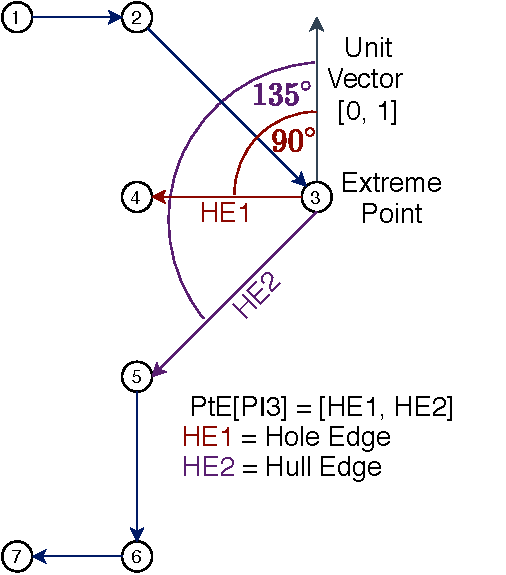
\includegraphics[width=.99\linewidth]{chapter_2_polylidar/imgs/EdgeHole.pdf}
%     \caption{}
%     \label{fig:ch2_example1_hole_extreme}
%   \end{subfigure}
%   \caption[Overview of boundary following procedure]{(a) Edge selection for Fig. \ref{fig:ch2_algorithm1_visual}a.  HE70 leads to point index PI10 during shell extraction. Half-edges HE28 and HE42 leave PI10. The correct edge to follow (HE42) has the greatest angle with HE70. (b) If the extreme point has two outgoing edges (HE1, HE2), choose the edge with largest angle difference with the unit vector [0,1]. This is edge HE2. }
%   \label{fig:ch2_example1} 
% \end{figure}


\begin{figure}[ht]
    \centering
  \begin{subfigure}[t]{.25\linewidth}
    \centering
    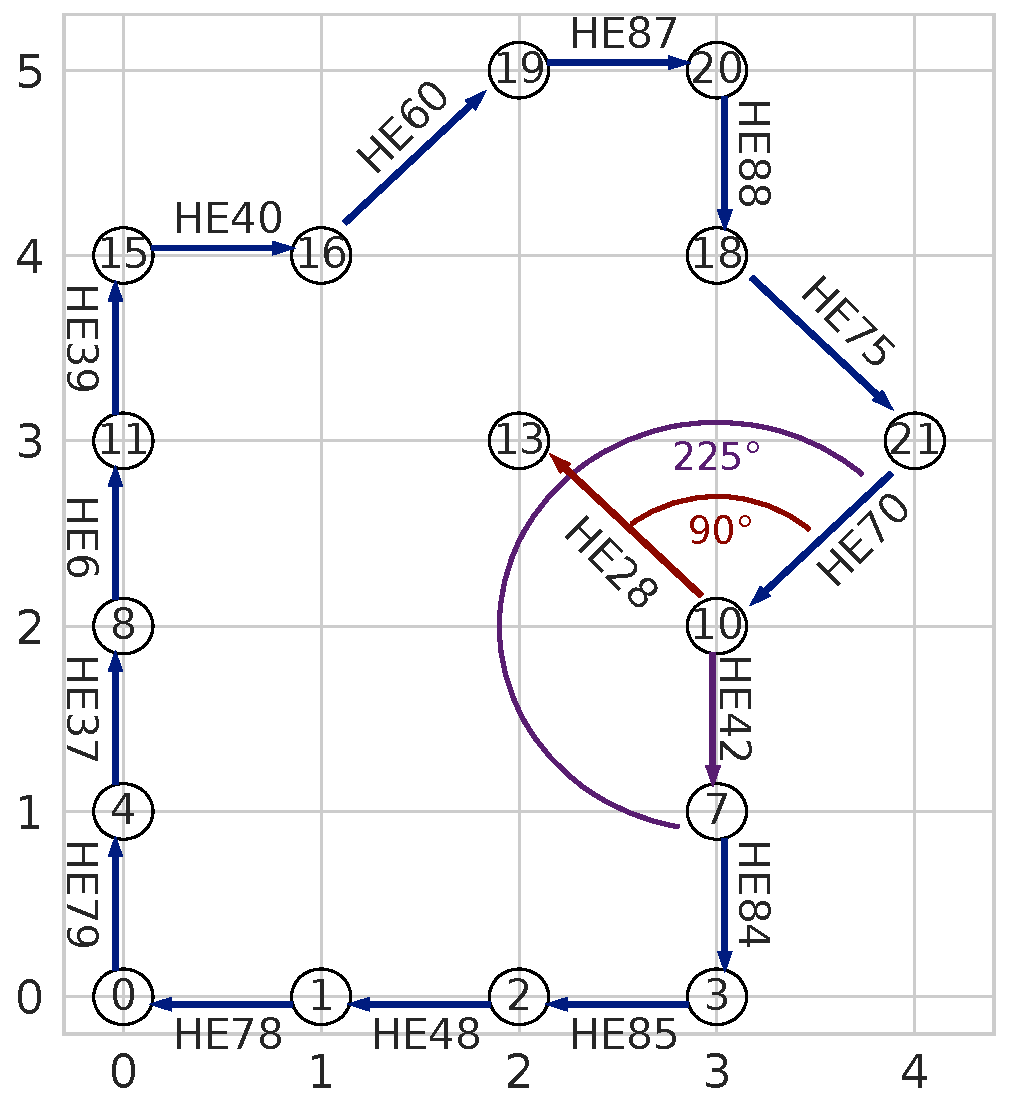
\includegraphics[width=0.99\linewidth]{chapter_2_polylidar/imgs/example_one_hole_choice_visual.pdf}
    \caption{}
    \label{fig:ch2_example1_non_extreme}
  \end{subfigure}
  \begin{subfigure}[t]{.23\linewidth}
    \centering
     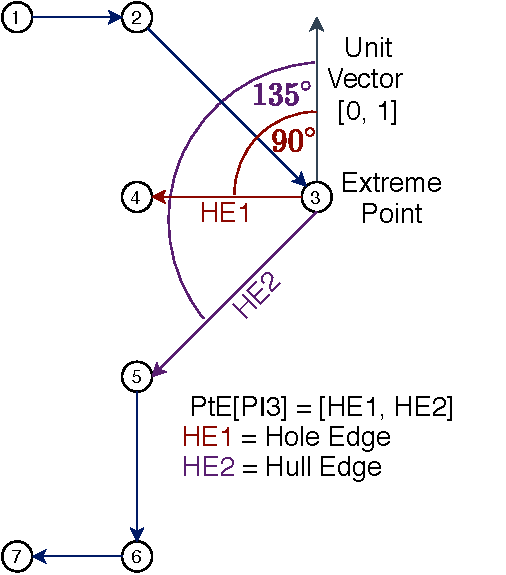
\includegraphics[width=.99\linewidth]{chapter_2_polylidar/imgs/EdgeHole.pdf}
    \caption{}
    \label{fig:ch2_example1_hole_extreme}
  \end{subfigure}
  \begin{subfigure}[t]{.25\linewidth}
    \centering
    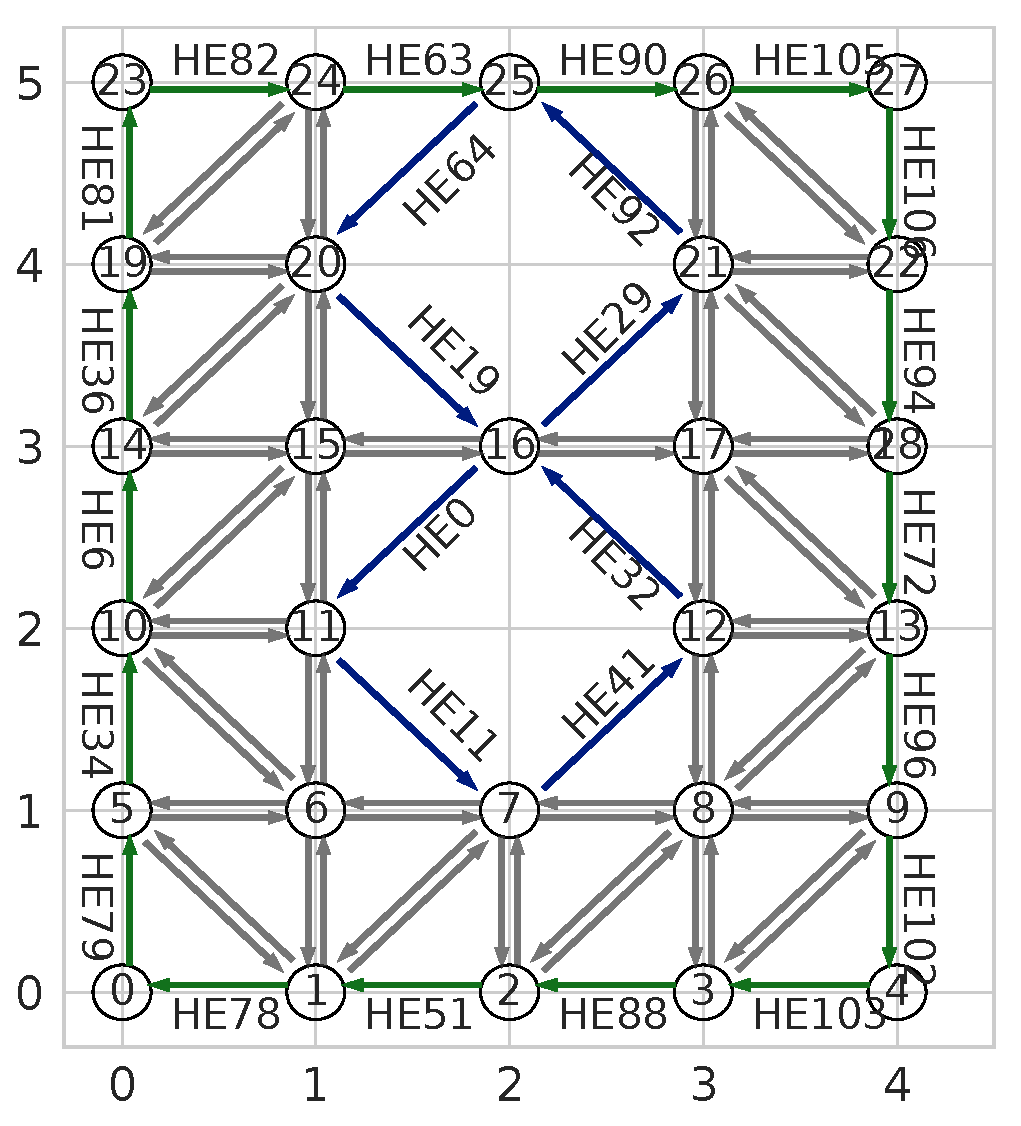
\includegraphics[width=0.99\linewidth]{chapter_2_polylidar/imgs/example_2_all.pdf}
    \caption{}
    \label{fig:ch2_example2_hull}
  \end{subfigure}
  \begin{subfigure}[t]{.25\linewidth}
    \centering
     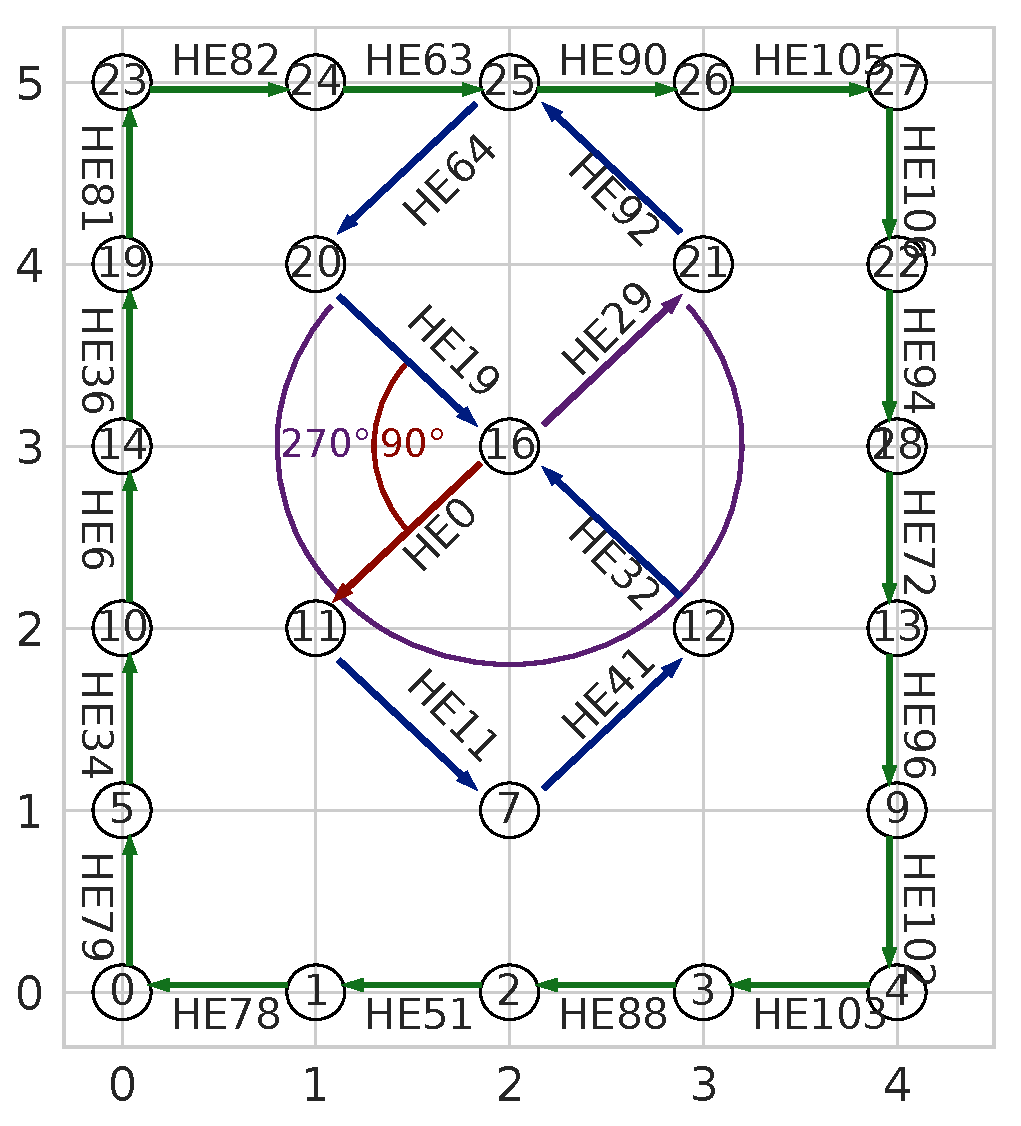
\includegraphics[width=.99\linewidth]{chapter_2_polylidar/imgs/example_2_choice.pdf}
    \caption{}
    \label{fig:ch2_example2_choice}
  \end{subfigure}
  \caption[Overview of boundary following procedure]{(a) Edge selection for Fig. \ref{fig:ch2_algorithm1_visual}a.  HE70 leads to point index PI10 during shell extraction. Half-edges HE28 and HE42 leave PI10. The correct edge to follow (HE42) has the greatest angle with HE70. (b) If the extreme point has two outgoing edges (HE1, HE2), choose the edge with largest angle difference with the unit vector [0,1]. This is edge HE2. (c) Edge case of two holes sharing the same vertex at PI16. The outer shell (green) is already extracted. (d) When traversing from HE19 to point index PI16, two outgoing edges (HE0 and HE29) are found. Edge HE29  with the largest angle difference from HE19 is chosen. }
  \label{fig:ch2_example1} 
\end{figure}


\subsubsection{Hole(s) Extraction}

After the outer shell of the concave hull has been determined, only the holes remain to be found (if any holes exist). Any edges that remains inside $\mathcal{BE}$ are hole edges and will be extracted using Algorithm \ref{alg:ch2_hole_extraction}.  A half-edge is randomly chosen from $\mathcal{BE}$ for which the same \texttt{ExtractLinearRing} procedure is run. Figure \ref{fig:ch2_example1}c shows a corner case of a non-manifold mesh that must be handled if two holes share the same vertex. The previously extracted concave shell is displayed in green while the remaining half-edges to be processed are in blue; note the shared vertex at PI16.  Figure \ref{fig:ch2_example1}d shows the event when HE19 is randomly chosen for hole extraction leading to PI16. HE0 or HE29 is chosen in the manner previously discussed: the edge with largest angle guarantees the smallest hole thus is chosen.  If the other edge was chosen this would indicate a hole inside a hole which is invalid.


\begin{algorithm}[ht]
    \SetKwInOut{Input}{Input}
    \SetKwInOut{Output}{Output}

    \Input{Half Edge Set , $\mathcal{BE} = \{he_i, \ldots, he_n\}$ \\ 
            Point Index Hash Map, $PtE$ \\
            Triangles Point Index, $triangles$
    }
    \Output{Set of Linear Ring Holes , $\mathcal{HR} = \{lr_1, \ldots, lr_k\}$ } 
    $\mathcal{HR} = \emptyset$  \tcc*{empty hole set}

    \While{$\mathcal{BE}$ is not empty}{

        $he= \operatorname{RandomChoice}(\mathcal{BE})$ \\
        $pi = triangles[he]$\\
        $lr = \operatorname{ExtractLinearRing}(\mathcal{BE}, PtE, he, pi, triangles)$ \\
    
        $\mathcal{HR} = \mathcal{HR} + lr$ 
    }
    return $\mathcal{HR}$
    \caption{Extract Holes}\label{alg:ch2_hole_extraction}
\end{algorithm}


% \begin{figure}[ht] 
%     \centering
%   \subfloat[]{%
%       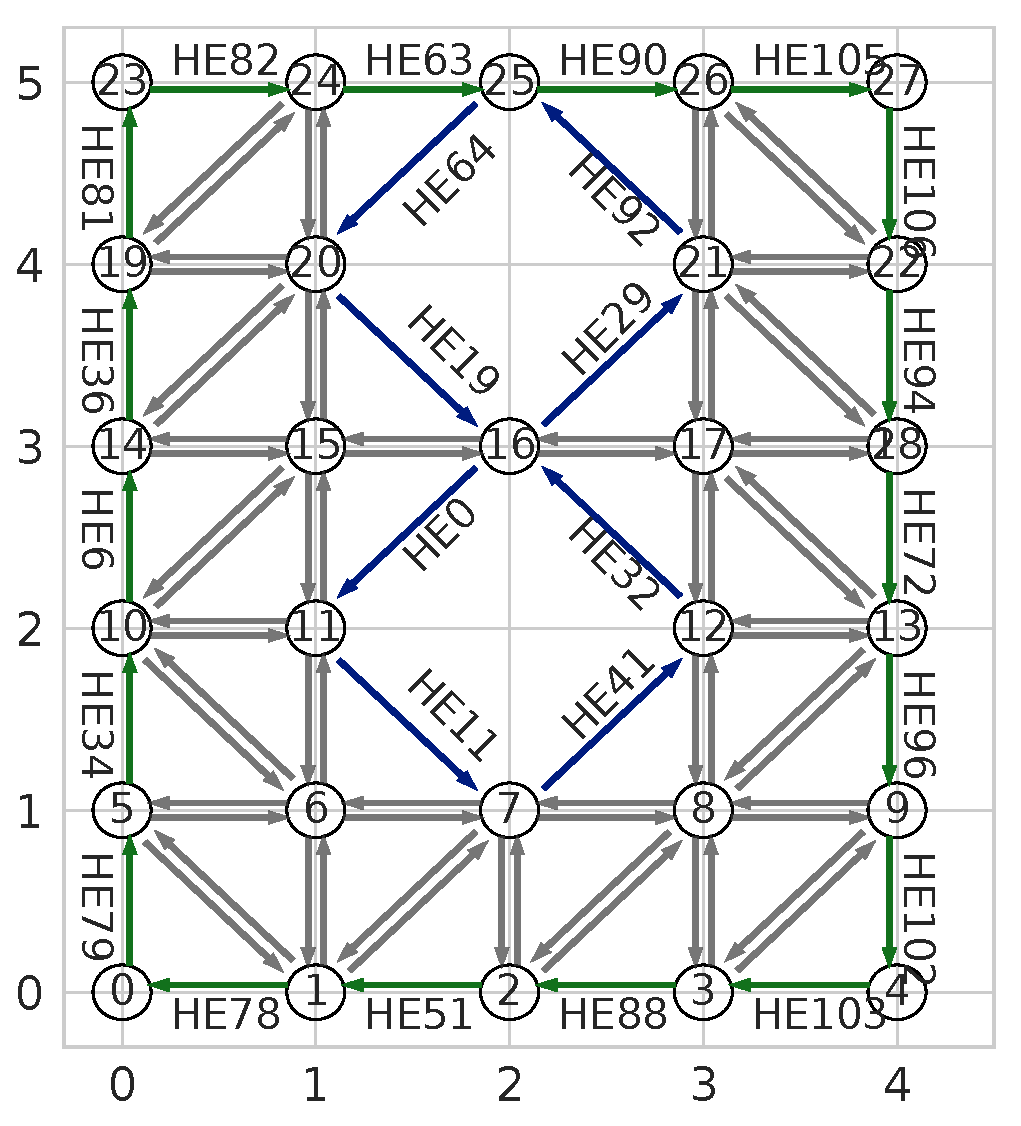
\includegraphics[width=0.45\linewidth]{chapter_2_polylidar/imgs/example_2_all.pdf}}
%     \label{fig:ch2_example2_hull}\hfill
%   \subfloat[]{%
%   \centering
%         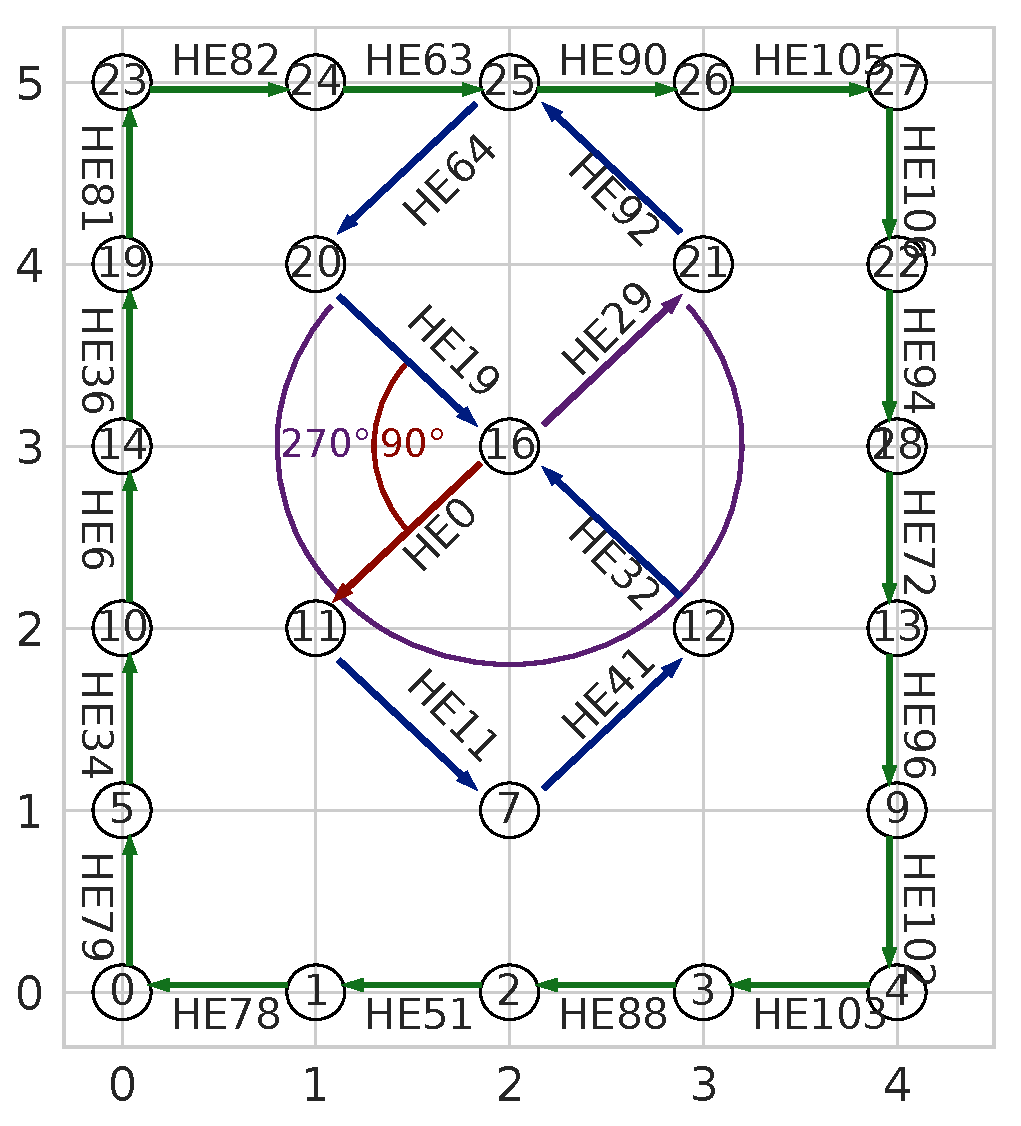
\includegraphics[width=.45\linewidth]{chapter_2_polylidar/imgs/example_2_choice.pdf}}
%     \label{fig:ch2_example2_choice}\\
%   \caption{(a) Edge case of two holes sharing the same vertex at PI16. The outer shell (green) is already extracted. (b) When traversing from HE19 to point index PI16, two outgoing edges (HE0 and HE29) are found. Edge HE29  with the largest angle difference from HE19 is chosen. }
%   \label{fig:ch2_example2} 
% \end{figure}


% \begin{figure}[ht]
%     \centering
%   \begin{subfigure}[t]{.25\linewidth}
%     \centering
%     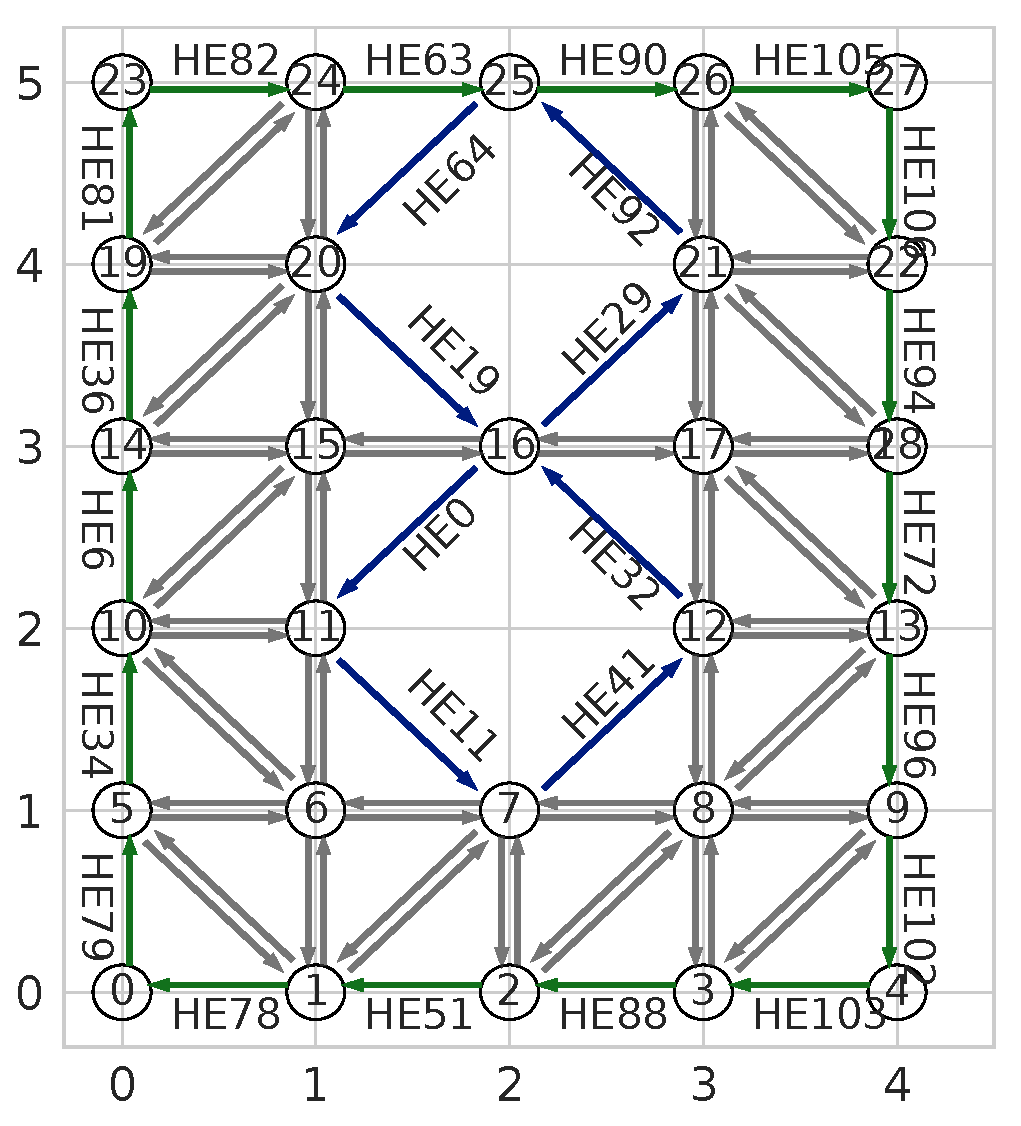
\includegraphics[width=0.99\linewidth]{chapter_2_polylidar/imgs/example_2_all.pdf}
%     \caption{}
%     \label{fig:ch2_example2_hull}
%   \end{subfigure}
%   \begin{subfigure}[t]{.25\linewidth}
%     \centering
%      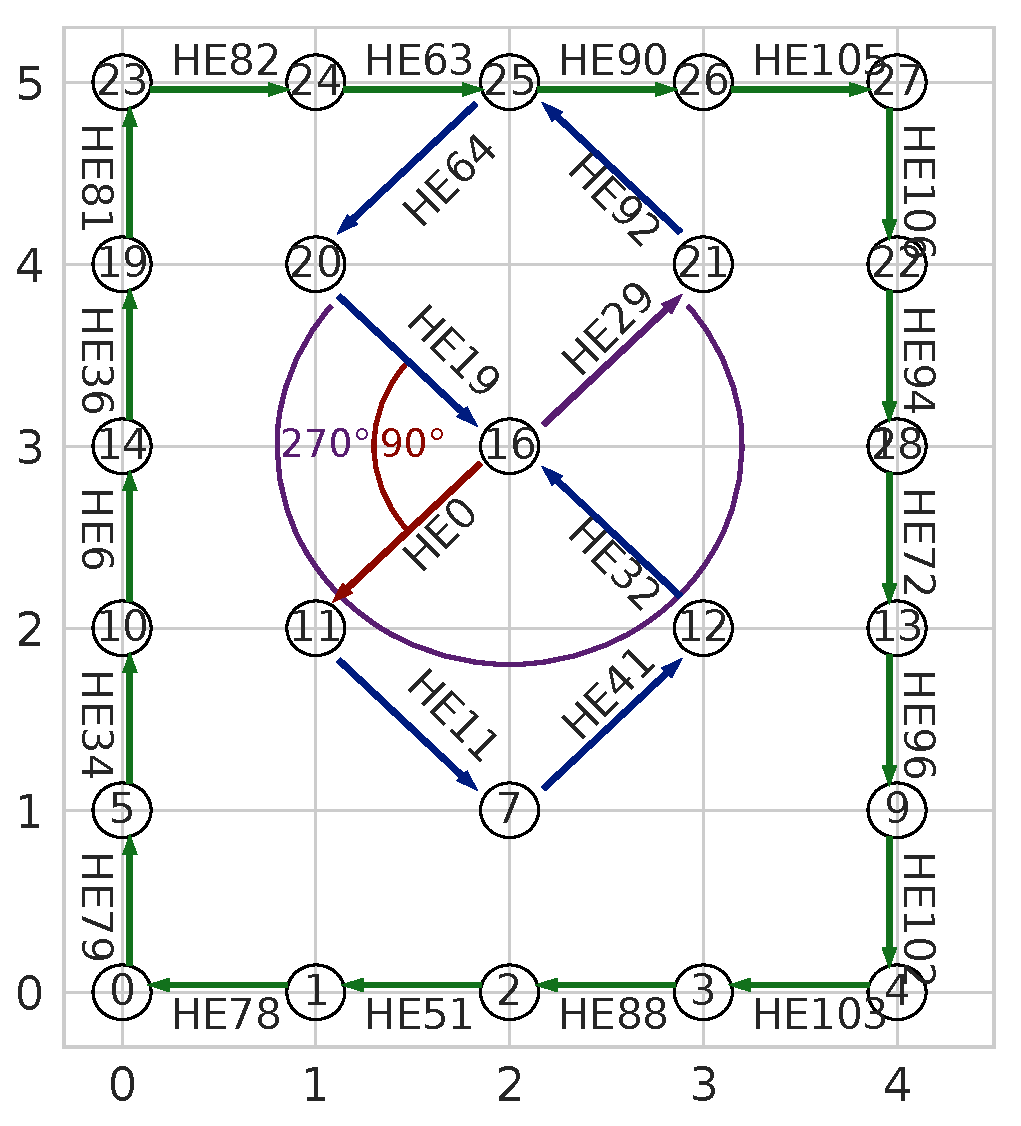
\includegraphics[width=.99\linewidth]{chapter_2_polylidar/imgs/example_2_choice.pdf}
%     \caption{}
%     \label{fig:ch2_example2_choice}
%   \end{subfigure}
%   \caption[Extracting a hole with a shared vertex]{(a) Edge case of two holes sharing the same vertex at PI16. The outer shell (green) is already extracted. (b) When traversing from HE19 to point index PI16, two outgoing edges (HE0 and HE29) are found. Edge HE29  with the largest angle difference from HE19 is chosen.}
%   \label{fig:ch2_example2} 
% \end{figure}





\subsection{Time Complexity}\label{sec:time_complexity}
This section describes the time complexity of Polylidar.
%, shown to be $\mathcal{O}(n\log{}n)$ where $n$ is the number of point cloud values in the point set.  
The Delaunay triangulation is first computed in $\mathcal{O}(n\log{}n)$ \cite{de_berg_delaunay_2008}. Region extraction from Section \ref{sec:ch2_mesh_extraction} is $\mathcal{O}(n)$:

\begin{itemize}
    \item At most $t = 2n - 2$ triangles are returned from Delaunay triangulation by Euler's formula so $t$ is linear in $n$.
    \item The maximum of $2*t$ iterations occurs. One loop filters triangles; worst case no triangles are removed. A second loop occurs over remaining connected triangles.
    \item Determining shared edges for expansion requires an $\mathcal{O}(1)$ lookup in the $halfedges$ array.
    \item Output generation $\mathcal{T}_{r}$ is $\mathcal{O}(1)$ for each insertion.
\end{itemize}

Polygon extraction is also $\mathcal{O}(n)$. The initialization procedure in Algorithm \ref{alg:ch2_boundary_edges} is $\mathcal{O}(n)$ per the following analysis:
\begin{itemize}
    \item Assuming the worst case, the algorithm loops through every edge of every triangle, providing a maximum number of iterations of $3 \cdot t$. Therefore the number of iterations is linear with $n$.
    \item Determining if an edge is a boundary edge is an $\mathcal{O}(1)$ operation. Line 6 is $\mathcal{O}(1)$ lookup in halfedges array. Line 8 is $\mathcal{O}(1)$ lookup in the input triangle set.
    \item Output generation, the half-edge set and point index hash map, is $\mathcal{O}(1)$ for each insertion.
\end{itemize}

Algorithm \ref{alg:ch2_concave_hull_shell} is linear in $n$ for similar reasons:
\begin{itemize}
    \item The number of iterations is the number of boundary edges computed, a subset of the iterations in Alg. \ref{alg:ch2_boundary_edges}.
    \item The output linear ring is $\mathcal{O}(1)$ for each insertion.
    \item The \texttt{SelectEdge} procedure is $\mathcal{O}(1)$ with no loops.
\end{itemize}

Finally Algorithm \ref{alg:ch2_hole_extraction} is also linear with respect to $n$. It is executed as many times as there are holes in a polygon. A hole contains a minimum of one triangle; we have shown previously that $t$ grows linearly with $n$. Selecting a random half-edge, Line 3, is an $\mathcal{O}(1)$ operation. Overall, Polylidar has complexity $\mathcal{O}(n\log{}n)$ from the initial triangulation.

\section{Benchmarking Comparisons}\label{sec:ch2_results}

This section benchmarks Polylidar against other common concave hull extraction methods which also extract holes; all code is open source\footnote{https://github.com/JeremyBYU/concavehull-evaluation}. Three other implementations are tested: CGAL's Alpha Shape function and the ST\_ConcaveHull function from PostGIS and Spatialite. For uniformity, Polylidar and CGAL are set to use the same $\alpha$ parameter to guarantee exact shape reproduction. Note that CGAL's Alpha Shape returns an unordered set of boundary edges; it does not convert these edges into a valid (multi)polygon. These edges produce the same shape as Polylidar when drawn on a canvas, but lack the desired polygon semantic data structure. PostGIS's concave hull implementation only returns single polygons, so MultiPolygon test cases are not evaluated against it. Both PostGIS and Spatialite are databases which require upload of the point set prior to algorithm execution; benchmark timing does not include data upload time. 
% Polylidar is configured to use fast adaptive precision floating point arithmetic for robust geometric predicates using \cite{shewchuk1997adaptive}.

% {\color{blue}
Section \ref{sec:ch2_rgbd} provides a benchmark from plane segmented point clouds produced by an RGBD camera. Section \ref{sec:ch2_state_shapes} generates synthetic 2D point sets from the state shapes of California (CA) and Hawaii (HI) to explore how the algorithms scale with respect to point size.  Section \ref{sec:ch2_alphabet_shapes} shows a similar benchmark but with the English alphabet. All utilize ground truth (multi)polygon shape $GT$ to evaluate shape accuracy. 
% Section \ref{sec:alphabet_shapes} comprehensively evaluates each algorithm for the 26 letters in the English alphabet (transformed to polygons), similarly to \cite{Duckham2008}.
% }
% Both sections use the test case as a ground truth (multi)polygon shape, $GT$, from which a 2D point set is uniformly sampled. 
Each implementation takes as input a point set and produces a concave shape, $CS$, which is similar to the ground truth polygon.  The $L^2$ error norm, the area of the symmetric difference between $GT$ and $CS$, is computed to enable evaluation of shape error $\frac{area((GT-CS) \cup (CS-GT))}{area(CS)}$. 
% provide good results, i.e.,

Each implementation contains its own parameter(s) modified to minimize $L^2$ error. Shape accuracy is therefore subject to parameter selection. Table \ref{table:ch2_params} displays the parameters chosen and used for all test cases (RGBD, CA, HI, Alphabet). Rows with two parameters separated by a semicolon indicate parameters for use with non-hole and hole cases.  Polylidar and CGAL use the same $\alpha$ parameter adjusted on a case by case basis. For each case we calculate point density $p_d$ and compute parameter $\alpha$ as $2p^{-1}_d$.  This gives reasonable but not necessarily optimal results.  Spatialite's concave hull implementation has  parameter $C$ which at its default value ($C=3$) produces excellent results. $C$ is adjusted as needed (for CA, HI) to further reduce error.  PostGIS' \emph{target percent} is set to provide the optimal accuracy based on  percent area reduction required. The most important takeaway when interpreting accuracy is thus trends in accuracy, not small numerical differences.


\begin{table}[ht]
\centering
\caption{Parameters for Test Cases}
\label{table:ch2_params}
\begin{tabular}{@{}cccccc@{}}
\toprule
Algorithm      & Parameter     & RGBD &       CA          & HI  &  Alph.                  \\ \midrule
CGAL/Polylidar & $\alpha$           & $2p^{-1}_d$  &$2p^{-1}_d$ & $2p^{-1}_d$ & $2p^{-1}_d$   \\ \addlinespace[1mm]
Spatialite     & $C$                & 3.0  &            2.0           & 2.0;1.3 & 3           \\
\addlinespace[1mm]
PostGIS        & $target$ \%  & Varies     & 0.76;0.72   & -         & Varies  \\ \bottomrule
\end{tabular}
\end{table}


\subsection{Plane Segmented Point Clouds from RGBD Images}\label{sec:ch2_rgbd}

Point clouds were generated with an Intel RealSense D435i camera at 424X240 resolution from eleven different scenes. Ten scenes were taken with the camera 1.5m above ground level pointing directly downward as shown in the top of Figure \ref{fig:ch2_realsense_benchmark}. Floor obstacle positions and orientations were changed in each scene.  The camera was placed higher and angled for the eleventh scene shown in the bottom of Figure \ref{fig:ch2_realsense_benchmark}. The floor can be quickly segmented using planar segmentation techniques \cite{feng_fast_2014, pham_geometrically_2016-1}. However for this experiment the floor was manually segmented, rotated to align with the XY image plane, and subsequently projected. This creates a 2D point set of the floors 3D point cloud. The ground truth polygon of each segmented point cloud was labeled by hand to provide accuracy scores.  The average size of the eleven segmented point clouds is 83,184 points. Table \ref{table:ch2_rgbd_results} displays the aggregate execution timings and accuracy results of all eleven points clouds for each algorithm. Polylidar is fastest. Polylidar, CGAL, and Spatialite have similar accuracies. Note that Polylidar and CGAL are configured to produce the same shape and therefore have the same $L^2$ error values.


\begin{table}[!ht]
\centering
\caption{RGBD Plane Segmented Point Clouds}
\label{table:ch2_rgbd_results}
\begin{tabular}{lcccccc}
\toprule
{} & \multicolumn{3}{c}{$L^2$ error \%} & \multicolumn{3}{c}{Time (ms)} \\
{Algorithm} &    mean & std &  max &      mean &     std &     max \\
% Algorithm        &         &     &      &           &         &         \\
\midrule
Polylidar  &           2.2   &   1.5 &      6.4 & 47.9 & 4.3 & 50.9  \\
CGAL       &           2.2 &    1.5 &      6.4 & 248.3 & 25.0 & 267.7        \\
PostGIS    &           7.5 & 1.6 & 9.9   & 2734.7 & 249.3 & 2939.9     \\
Spatialite &           2.2 & 1.5 & 6.3 &  13333.0 & 2486.6  &   16386.5 \\
\bottomrule
\end{tabular}
\end{table}

\begin{figure}[ht] 
    \centering
      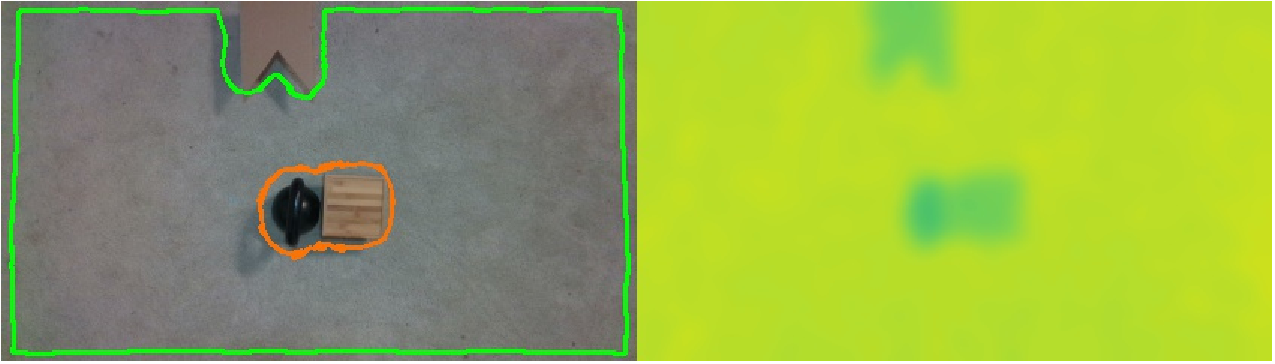
\includegraphics[width=0.80\linewidth]{chapter_2_polylidar/imgs/RealSensePictures-scene_08_stack.pdf}
      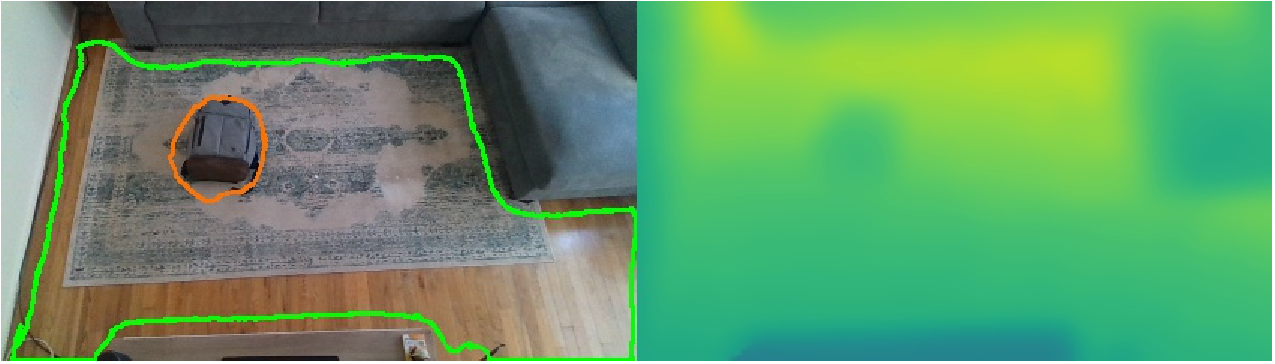
\includegraphics[width=0.80\linewidth]{chapter_2_polylidar/imgs/RealSensePictures-scene_11_stack.pdf}
  \caption[Extracting a polygon from a plane-segmented RGBD point cloud]{Two example scenes (top/bottom) from RGBD benchmark. A point cloud is generated from depth image (right) and manually segmented to include only the ground floor. The polygonal output of Polylidar is shown in the RGB image (left). Green is the hull, orange represents holes. }
  \label{fig:ch2_realsense_benchmark} 
\end{figure}

\subsection{State Shapes}\label{sec:ch2_state_shapes}

Figure \ref{fig:ch2_compare_algs_all} shows CA and HI test case geometries (first column), execution times (second column), and error results (third column). Each state shape is processed with and without random holes
%to verify each implementation's ability to handle hole extraction.
; dashed lines indicate results where holes are included in the ground truth polygon. Point sets are randomly sampled from the state shapes. Each test was run 10 times with input point set sizes ranging from (2, 4, 8, 16, 32, 64) thousand points with mean timing and error plotted. Confidence intervals are provided for execution timing, however they are almost imperceptible because the variance is low at this scale. Polylidar and CGAL are significantly faster than the other methods, with Spatialite having the slowest implementation. An inset (zoomed) box that focuses solely on CGAL and Polylidar is shown in the second column, showing that on average Polylidar is $\sim4$ times faster than CGAL. 
% Spatialite's slow speed is attributed to unioning triangles to determine final polygon shape as determined through profiling \cite{pprof}.
The presence of holes affected each method differently: decreased time in Spatialite (fewer triangles to union), increased time for PostGIS (a decrease in \emph{target percent} increases run-time). No significant changes were noted for CGAL and Polylidar.  

%$L^2$ error (Figure \ref{fig:compare_algs_all}c,f,i. 
%Polylidar and CGAL are configured to produce the same shape and therefore have the same $L^2$ error. 
Spatialite produced shapes with the least error, followed by Polylidar/CGAL and then PostGIS.  Spatialite has the lowest error because it incorporates triangle edge length statistics into its triangle filtering which better handles random sampling. In contrast, Polylidar/CGAL offer comparable accuracies with RGBD data due to the more uniform point distribution in top-down RGBD imagery. PostGIS error increased markedly with holes since it did not accurately reproduce them. 
%Though technically possible, it seems difficult for PostGIS to reproduce holes in dense point sets. 
Figure \ref{fig:ch2_ca_output} shows a visual comparison of CA concave polygon outputs for each algorithm. 
% The figure caption already says this --> when run on a 4000 point set sampled from CA in Figure \ref{fig:compare_algs_all}d. 


\begin{figure}[ht]
    \centering
  \begin{subfigure}[t]{.28\linewidth}
    \centering
    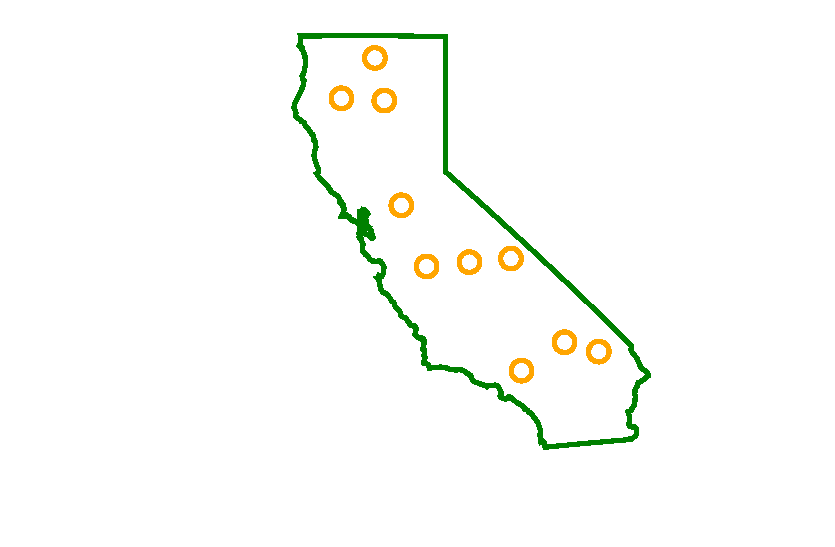
\includegraphics[clip, trim=1.5cm 0cm 1.5cm 0cm, width=0.99\linewidth]{chapter_2_polylidar/imgs/caholes.pdf}
    \caption{}
    \label{fig:ch2_ca_holes}
  \end{subfigure}
  \begin{subfigure}[t]{.36\linewidth}
    \centering
     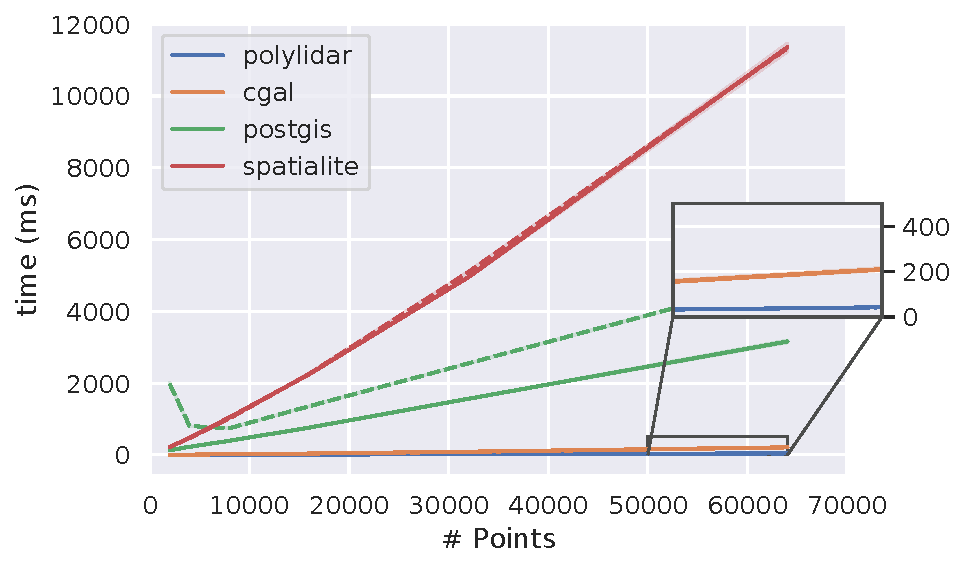
\includegraphics[width=.99\linewidth]{chapter_2_polylidar/imgs/compare_algs_time_inset_ca.pdf}
    \caption{}
    \label{fig:ch2_ca_tim}
  \end{subfigure}
  \begin{subfigure}[t]{.33\linewidth}
    \centering
    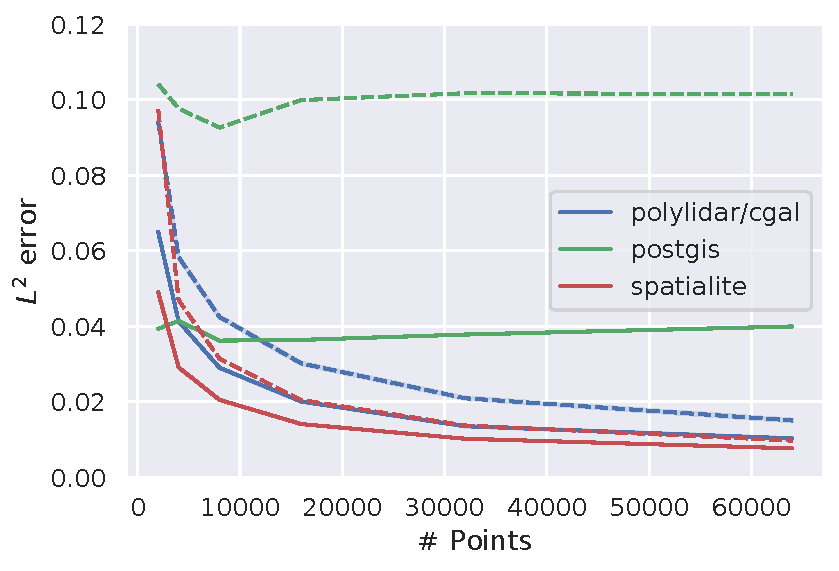
\includegraphics[width=.99\linewidth]{chapter_2_polylidar/imgs/compare_algs_accuracy_ca-min.pdf}
    \caption{}
    \label{fig:ch2_ca_acc}
  \end{subfigure}
  \begin{subfigure}[t]{.28\linewidth}
    \centering
    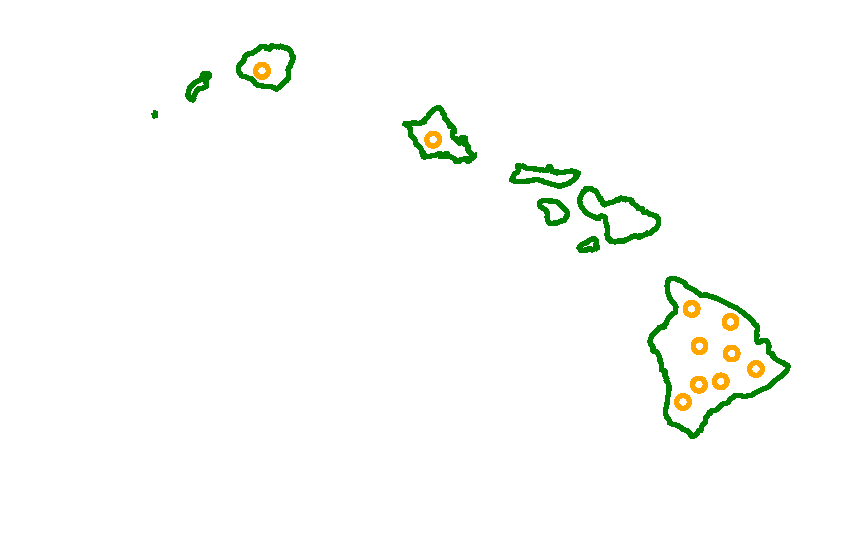
\includegraphics[clip, trim=1.5cm 0cm 1.0cm 0cm, width=0.99\linewidth]{chapter_2_polylidar/imgs/hiholes.pdf}
    \caption{}
    \label{fig:ch2_hi_holes}
  \end{subfigure}
  \begin{subfigure}[t]{.36\linewidth}
    \centering
     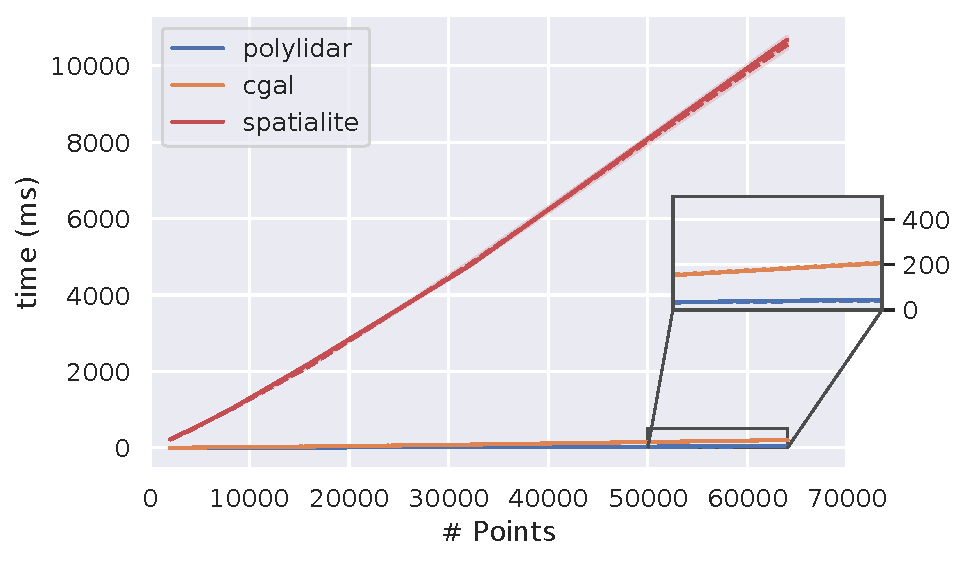
\includegraphics[width=.99\linewidth]{chapter_2_polylidar/imgs/compare_algs_time_inset_hi.pdf}
    \caption{}
    \label{fig:ch2_hi_tim}
  \end{subfigure}
  \begin{subfigure}[t]{.33\linewidth}
    \centering
    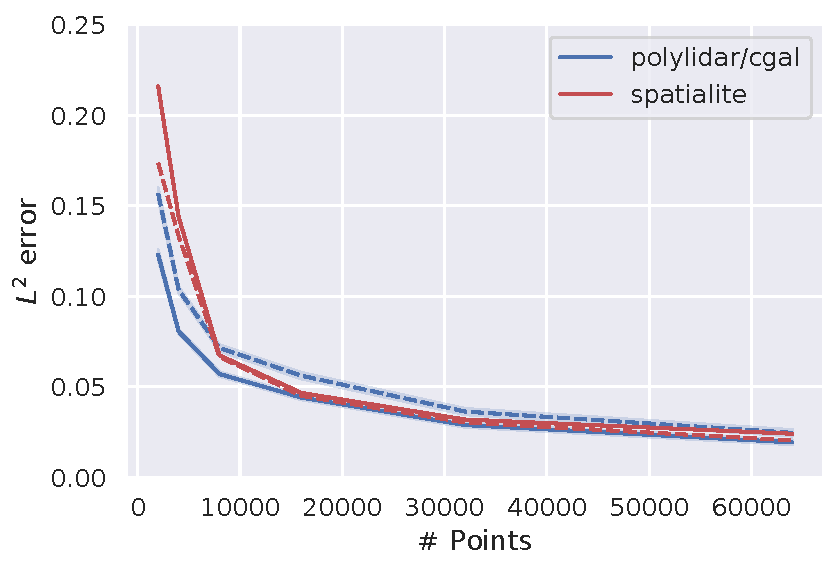
\includegraphics[width=.99\linewidth]{chapter_2_polylidar/imgs/compare_algs_accuracy_hi-min.pdf}
    \caption{}
    \label{fig:ch2_hi_acc}
  \end{subfigure}
  \caption[Execution and accuracy results from state shape benchmark]{Concave hull extraction results. Rows from top to bottom correspond to outlines of California (CA) (a, b, c), and Hawaii (HI) (d, e, f) with random holes inserted. The first column shows ground truth polygons with circular holes in orange. The second column shows execution time as a function of number of 2D points provided. The third column shows shape error as a function of number of 2D points provided. Dashed lines show results where holes were placed inside the polygon outline, while solid lines show results with no holes. PostGIS cannot handle MultiPolygons thus was not tested for HI.}
  \label{fig:ch2_compare_algs_all} 
\end{figure}

\begin{figure}[!ht] 
    \centering
      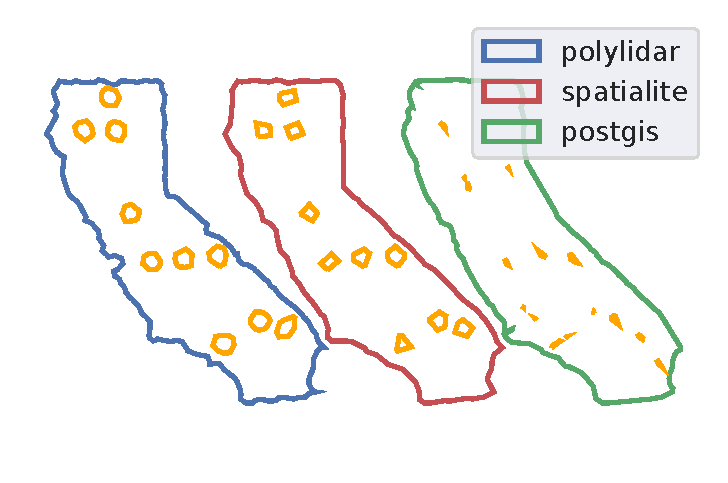
\includegraphics[clip, trim=0.5cm 1.2cm 0.0cm 0.0cm, width=0.35\linewidth]{chapter_2_polylidar/imgs/ouput_ca.pdf}
  \caption[Visual comparison of different polygon extraction methods]{Concave polygon output from Polylidar/CGAL (left), Spatialite (center), and PostGIS (right).  Input to each algorithm was a 4000 point set sampled from the California (CA) polygon with holes per Figure \ref{fig:ch2_compare_algs_all}a.}
  \label{fig:ch2_ca_output} 
\end{figure}





\subsection{Alphabet Shapes}\label{sec:ch2_alphabet_shapes}

% {\color{blue}
Polygons from 26 capital letters of the English alphabet were generated and 2000 points randomly sampled inside.
%Some polygon letters naturally have holes such as ``A'', however no capital letters are MultiPolygons. Each letter was uniformly sampled to generate a 2000 point set and run through each algorithm. 
The ``A'' in Figure \ref{fig:ch2_convex_concave}b shows an example capital letter with the output of Polylidar's concave hull. Table \ref{table:ch2_alphabet_tests} provides aggregate statistics of all 26 test cases. Polylidar continues to lead in speed. Spatialite leads in accuracy by a marginal amount. The alphabet shapes are significantly more concave than previous benchmarks. Documentation of PostGIS indicates that the run time grows quadratically as concavity increases leading to the high execution times observed \cite{open_source_geospatial_foundation_postgis_2019}.

%However PostGIS shape error and time are significantly higher than previously seen. This is because the alphabet shapes are significantly more concave then the tested state shapes, requiring a much smaller \emph{target percent} parameter for PostGIS (on average 0.38). Documentation of PostGIS indicates that the run time grows quadratically when reducing this parameter and at ``small'' values may fail to produce a concave shape \cite{postgis}.  PostGIS failed to produce any shape for the letters ``J'', ``L'', and ``M''. All other algorithms provided valid results for all test cases.
%  (reduced to 1000 points for visual clarity)

%  Polylidar continues to lead in speed, about 4.5 times faster than the next leading algorithm CGAL (shape error remains the same because of same $\alpha$ used). Spatialite continues to lead in accuracy by a marginal amount for the same reasons discussed previously. However PostGIS shape error and time are significantly higher than previously seen. This is because the alphabet shapes are significantly more concave then the tested state shapes, requiring a much smaller \emph{target percent} parameter for PostGIS (on average 0.38). 
% Documentation of PostGIS indicates that the run time grows quadratically when reducing this parameter and at ``small'' values may fail to produce a concave shape \cite{postgis}.  PostGIS failed to produce any shape for the letters ``J'', ``L'', and ``M''. All other algorithms provided valid results for all test cases.
% }
 
\begin{table}[!ht]
\centering
\caption{Alphabet Letter Results, 26 Shapes}
\label{table:ch2_alphabet_tests}
\begin{tabular}{lcccccc}
\toprule
{} & \multicolumn{3}{c}{$L^2$ error \%} & \multicolumn{3}{c}{Time (ms)} \\
{Algorithm} &    mean & std &  max &      mean &     std &     max \\
% Algorithm        &         &     &      &           &         &         \\
\midrule
% polylidar  &    12.8 & 1.8 & 16.8 &       1.8 &     0.3 &     2.9 \\
% cgal       &    12.8 & 1.8 & 16.8 &       6.8 &     0.8 &     9.8 \\
% postgis    &    36.5 & 9.9 & 53.7 &   18973.3 & 10786.2 & 39587.8 \\
% spatialite &    11.2 & 4.5 & 22.1 &     330.4 &    33.8 &   438.1 \\
Polylidar  &           12.8 & 1.8 & 16.8 &       1.2 &    0.3 &     2.4 \\
CGAL       &           12.8 & 1.8 & 16.8 &       5.4 &    0.9 &     7.2 \\
PostGIS    &           36.5 & 9.9 & 53.7 &   13091.8 & 7500.6 & 28451.0 \\
Spatialite &           11.2 & 4.5 & 22.1 &     230.2 &    6.3 &   242.9 \\
\bottomrule
\end{tabular}
\end{table}

\section{Random Polygon Tests}\label{sec:ch2_random_polygons_test}
More than 19,600 polygons were randomly generated to test Polylidar. Half the test cases had random holes.  Polygon complexity is characterized by convexity metric $$CV = \frac{Area(P)}{Area(CH(P))}$$
\noindent where $P$ is the polygon and $CH()$ is the convex hull function. A convexity of 1 indicates the sample polygon is its convex hull.
% Point sets of size 2,000 and 8,000 were randomly sampled for each polygon and input to Polylidar with the $\alpha$ parameter from Table
8,000 points were randomly sampled for each polygon and input to Polylidar with the $\alpha$ parameter from Table
\ref{table:ch2_params}.  Execution time and accuracy are summarized in Table \ref{table:ch2_random_tests}. The table is partitioned into high, medium, and low ground truth polygon convexity defined by $CV \geq 0.75$, $0.75 < CV \geq 0.55$, and $CV < 0.55$ respectively. 
%Figure \ref{fig:convexity} illustrates the impact of $CV$ value on polygon shape. Note that the CA polygon has a  $CV=0.74$.
Every polygon produced by Polylidar was confirmed valid independently by the GEOS geometry library.
% In all examples we find that greater point density improves Polylidar accuracy.  
As polygon convexity ($CV$) decreases Polylidar shape estimation accuracy also decreases. Polygons in our ``low'' convexity class have extremely non-convex shapes, the lowest with $CV=0.26$ per Figure \ref{fig:ch2_convexity}.

\begin{table}[ht!]
\centering
\caption{Random Tests; $CV$ = Convexity Metric}
\label{table:ch2_random_tests}
\begin{tabular}{@{}lcccccc@{}}
\toprule
    &    \multicolumn{3}{c}{$L^2$ error \%} & \multicolumn{3}{c}{Time (ms)} \\
$CV$  &    mean & std &  max &      mean & std &  max \\
% $CV$ & points &         &     &      &           &     &      \\
\midrule
% hi & 2000 &     8.4 & 1.0 & 11.6 &       1.1 & 0.0 & 1.5 \\
%     & 8000 &     4.4 & 0.5 &  6.1 &       4.6 & 0.1 & 5.0 \\
% mid & 2000 &    15.1 & 2.0 & 23.7 &       1.1 & 0.0 & 1.7 \\
%     & 8000 &     8.0 & 1.1 & 13.0 &       4.6 & 0.1 & 8.1 \\
% low & 2000 &    28.3 & 5.1 & 43.6 &       1.1 & 0.0 & 1.3 \\
%     & 8000 &    15.5 & 3.0 & 25.0 &       4.7 & 0.2 & 9.9 \\
% hi & 2000 &     8.4 & 1.0 & 11.6 &       1.1 & 0.0 & 1.5 \\

hi    &     4.4 & 0.5 &  6.1 &       4.6 & 0.1 & 5.0 \\
mid   &     8.0 & 1.1 & 13.0 &       4.6 & 0.1 & 8.1 \\
low   &    15.5 & 3.0 & 25.0 &       4.7 & 0.2 & 9.9 \\
\bottomrule
\end{tabular}
\end{table}

% \begin{figure}[!ht] 
%     \centering
%   \subfloat[]{%
%       
\includegraphics[width=0.38\linewidth]{chapter_2_polylidar/imgs/hi_convexity.pdf}}
%     \label{fig:ch2_hi_convexity}\hfill
%   \subfloat[]{%
%         
\includegraphics[width=.38\linewidth]{chapter_2_polylidar/imgs/low_convexity.pdf}}
%     \label{fig:ch2_low_convexity}\\
%   \caption{(a) Example of a high convexity polygon; CV = 86.1\% (b)  and a low convexity polygon; CV = 26.2\%}
%   \label{fig:ch2_convexity} 
% \end{figure}

\begin{figure}[ht]
    \centering
  \begin{subfigure}[t]{.25\linewidth}
    \centering
    
\includegraphics[width=0.99\linewidth]{chapter_2_polylidar/imgs/hi_convexity.pdf}
    \caption{}
    \label{fig:ch2_hi_convexity}
  \end{subfigure}
  \begin{subfigure}[t]{.26\linewidth}
    \centering
     
\includegraphics[width=.99\linewidth]{chapter_2_polylidar/imgs/low_convexity.pdf}
    \caption{}
    \label{fig:ch2_low_convexity}
  \end{subfigure}
  \caption[Example of high and low convexity polygons]{(a) Example of a high convexity polygon; CV = 86.1\% (b)  and a low convexity polygon; CV = 26.2\%}
  \label{fig:ch2_convexity} 
\end{figure}


\section{Discussion}\label{sec:ch2_discussion}
The benchmarks above indicate that Polylidar is the faster concave (multi)polygon extraction algorithm with the possibility of holes. This section discusses why Polylidar was faster in comparison to others. We specifically analyze the execution time of the major steps in Polylidar in comparison to other triangulation-based methods, namely CGAL and Spatialite. The three major steps are:

\begin{enumerate}
    \item Triangulation - The point set is triangulated creating a mesh of faces, edges, and vertices.
    \item Shape Extraction - Mesh simplices are removed based upon the $\alpha$ parameter or edge length. Remaining triangles, edges, and vertices represent the ``shape".
    \item Polygon Extraction - The ``shape" is converted to a (multi)polygon with the possibility of holes.
\end{enumerate}

\textbf{Triangulation} All perform Delaunay triangulation using robust geometric predicates but use different libraries to do so. Polylidar uses Delaunator, CGAL uses its own 2D triangulation, and Spatialite uses GEOS. 

\textbf{Shape Extraction} Polylidar and Spatialite are most similar, focusing only on filtering triangles in the mesh. However Polylidar goes further with region growing (Section \ref{sec:ch2_mesh_extraction}) that isolates disconnected regions in the mesh. For memory efficiency and speed we represent the filtered triangle set $\mathcal{T}_f$ as a bit array with 1/0 indicating in/out of set. This allows rapid triangle filtering and region growing which was previously profiled to be slower when using hashmaps. On the other hand CGAL first creates ``interval hashmaps'' for its simplices, including triangles, edges, and vertices.  These hashmaps store data detailing at what $\alpha$-interval a specific simplex would be in the $\alpha$-complex. These ordered hashmaps give the ability to more quickly compute a \emph{family} of $\alpha$-shapes from a point set. These data structures are implemented as C++ multimaps with $\mathcal{O}(\log{}n)$ for insertion/look-up in comparison to unordered maps having $\mathcal{O}(1)$. This design choice leads to shape extraction having an $\mathcal{O}(n \log{}n)$ complexity for CGAL. By creating hash maps for edges and vertices CGAL can also return the \emph{singular} points and edges which are isolated and not attached to any triangle in the $\alpha$-complex (e.g., a single point far removed from all others). Polylidar need not do this because singular points and edges cannot be polygons thus are not required steps in shape extraction.

\textbf{Polygon Extraction} Polylidar independently converts each region into a polygon. Algorithm 2 quickly identifies all border edges and uses efficient unordered contiguous memory hashmaps to store this information in $\mathcal{BE}$ and $PtE$. The essence of Algorithms 3 and 4 are entirely border-edge based leading to a significant speed up compared to triangle based methods (i.e., perimeter vs. area).  Spatialite uses GEOS to take the union of all unfiltered triangles to generate a valid multipolygon. CGAL's Alpha Shape produces an unordered list of the boundary edges of the $\alpha$-shape. However CGAL does not provide any explicit function to convert this list to a valid (multi)polygon. 
% These algorithms perform boundary following to properly extract the LinearRing(s) of the outer shell and hole(s).
%The authors are unaware of any other polygon extraction methods performing boundary following (while handling holes) as outlined in Algorithms 3 and 4.

% , i.e., the quantity of border edges is generally significantly lower than the number of interior triangles.


\begin{table}[ht]
\centering
\caption{Algorithm Timings - Mean of 30 runs in milliseconds}
\label{table:ch2_disc_subtimings}
\begin{tabular}{@{}ccccc@{}}
\toprule
\multirow{2}{*}{Algorithm} & \multirow{2}{*}{triangulation} & \multirow{2}{*}{\begin{tabular}[c]{@{}c@{}}shape\\ extraction\end{tabular}} & \multirow{2}{*}{\begin{tabular}[c]{@{}c@{}}polygon\\ extraction\end{tabular}} & \multirow{2}{*}{total} \\
                          &                                &                                                                             &                                                                               &                        \\ \midrule
Polylidar                  & 36.0                           & 4.4                                                                         & 1.0                                                                           & 41.4                   \\
CGAL                       & 44.5                           & 154.0                                                                       & --                                                                            & 198.5                  \\
Spatialite                 & 234.2                          & 135.3                                                                       & 10788.7                                                                       & 11158.1                \\ \bottomrule
\end{tabular}
\end{table}


Table \ref{table:ch2_disc_subtimings} summarizes mean execution timings for each of the main steps for Polylidar, CGAL, and Spatialite. The 64,000 point set in the shape of California (with holes) is used, with each algorithm executed 30 times with the mean presented.  Relative execution times with other point sets are similar.  Delaunator in Polylidar triangulated this specific point set fastest with CGAL a close second. Polylidar achieves a more significant speed-up in shape extraction for which Polylidar is 35 and 32 times faster than CGAL and Spatialite, respectively. Also, Polylidar's polygon extraction is about four orders of magnitude faster than Spatialite whereas CGAL does not extract polygons. CGAL instead offers a general purpose $\alpha$-shape construction routine to compute a family of shapes from different $\alpha$-values. %Polylidar is focused entirely on the end goal of generating \emph{polygons} given user parameters and a point set. It only uses boundary-edges for polygonizaton of the extracted shape, whereas Spatialite uses triangles. 

%  } %blue color 


% Primary Datastructures: Triangle Set is represented as an array of bits, 1/0 = in/not-in set

\section{Conclusion}\label{sec:ch2_conclusion}

This chapter has introduced Polylidar, an efficient 2D concave hull extraction algorithm which produces (multi)polygon output with holes. Comparison benchmarks of numerous test sets, similarly done in \cite{duckham_efficient_2008}, show Polylidar is faster than competing approaches with comparable or better accuracy. Additionally we perform random polygon tests that confirm every polygon produced by Polylidar is valid. In future work we will extend Polylidar to operate directly on 3D point cloud data by performing both planar segmentation and polygon extraction. We will remove Polylidar's reliance on Delaunay triangulation when used with organized point clouds (e.g., range images) similar to \cite{lee_fast_2013}. Triangulation can be performed in $\mathcal{O}(n)$ time by exploiting the spatial relationship inherit in range images. The OpenMP library will be used to parallelize iteration independent loops such as triangle filtering. Additionally we will explore task-based parallelization by making use of the data independence between polygons, i.e., spawning polygon extraction tasks immediately after a plane is segmented \cite{huang_cpp-taskflow_2019}. 
 
\chapter{Polygons from 3D Data}
 \label{ch:polylidar3d}
 \section{Introduction}
Flat surfaces are pervasive in engineered structures and also occur in natural terrain. For~example, structures such as walls, floors, rooftops, and~roadways are often flat or ``flat-like''. Similarly, home~and office furnishings are typically composed of multiple flat surfaces. Sensors such as LiDAR and \ac{RGBD} cameras generate dense 3D point clouds of these predominately flat surface environments. This observation has been exploited for tasks in localization and mapping~\cite{pathak_online_2010}, digital preservation with Photogrammetry and laser scanning \cite{malihi_3d_2016, lerma_terrestrial_2010, balsa-barreiro_generation_2018}, and~point cloud registration~\cite{rusinkiewicz_efficient_2001}. Planar~segmentation techniques are often used to group points together belonging to a flat surface~\cite{feng_fast_2014, pham_geometrically_2016-1, schaefer_maximum_2019}. However~points clouds are dense incurring a high computational cost when used directly in higher level tasks.~Planar~point clouds can be converted to lower dimensional representations such as polygons.~Polygons~reduce map size, accelerate matching for localization~\cite{lee_indoor_2012-1}, and~support model reconstruction and object detection~\cite{cao_roof_2017}. 

Planar points clouds may be converted to convex polygons~\cite{biswas_planar_2012}. Convex polygons are simple and efficient to generate but often do not represent the true shape of a point set. Non-convex polygons may be generated using techniques such as $\alpha$-shapes but operate strictly on 2D data, requiring the projection of each 3D planar point cloud and expensive triangulation~\cite{lee_fast_2013, edelsbrunner_shape_1983}. Pixel-level boundary following of organized point clouds can be used to extract non-convex polygons but often only captures the exterior shell of the polygon~\cite{lee_indoor_2012-1}. These methods are not able to capture \emph{interior} holes in a polygon representing the shape of obstacles on flat surfaces. Finally, speed is an important consideration for many of the applications mentioned previously. Parallel algorithms written for multi-core CPUs and GPUs should be used to reduce~latency. 

% JC_Author: It's important that this figure is not too small. The edit of changing to "width=0.7" makes the text not legible. It should be a minimum of 0.85 as it is now.
\begin{figure}[t]
    \centering
    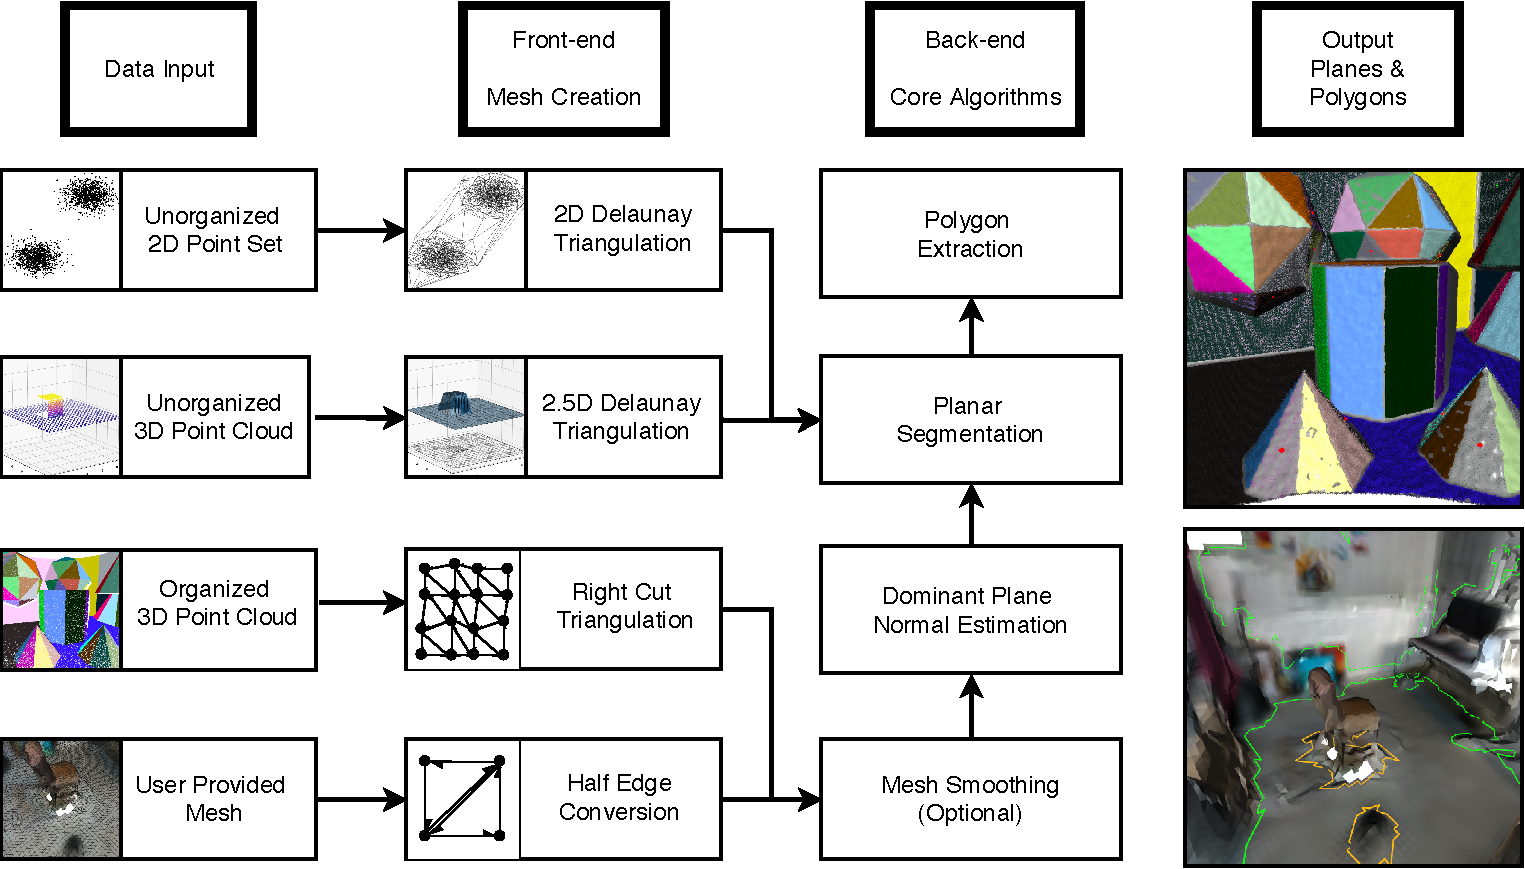
\includegraphics[width=0.95\linewidth]{chapter_3_polylidar3d/imgs/Polylidar3DArchitecture-SimplifedV4.pdf}
    \caption[Overview of Polylidar3D's data input, algorithms, and output]{Overview of Polylidar3D. Input data can be 2D point sets, unorganized/organized 3D point clouds, or~user-provided meshes. Polylidar3D's front-end transforms input data to a half-edge triangulation structure. The~back-end is responsible for mesh smoothing, dominant plane normal~estimation, planar segmentation, and~polygon extraction. Polylidar3D outputs both planes (sets of spatially connected triangles) and corresponding polygonal representations. An~example output of color-coded extracted planes from organized point clouds is shown (top right). An~example of extracted polygons from a user-provided mesh is shown (bottom right). The~green line represents the concave hull; orange lines show interior holes representing obstacles.} %Note that only one planar direction can be extracted for unorganized 3D point clouds. This is suitable for airborne LiDAR point~clouds. }
    \label{fig:ch3_polylidar_overview}
\end{figure}

This chapter presents Polylidar3D, a~non-convex polygon extraction algorithm which takes as input either unorganized 3D point clouds (e.g., airborne LiDAR point clouds), organized point clouds (e.g.,~range~images), or~user provided meshes. The~non-convex polygons extracted represent flat surfaces in an environment, while interior holes represent obstacles on these surfaces.~Figure~\ref{fig:ch3_polylidar_overview}~provides an overview of Polylidar3D's data input, front-end, back-end, and~output.  Currently only one planar direction can be extracted from unorganized 3D point clouds while all other 3D data inputs do not have this limitation. The~front-end transforms input data into a half-edge triangular mesh.  This~representation provides a common level of abstraction offering increased efficiency for back-end operations. The~back-end is composed of four core algorithms: mesh smoothing, dominant plane normal estimation, planar segment extraction, and~polygon extraction.  Polylidar3D outputs planar triangular segments, sets of flat connected triangles, and~their polygonal representations. Polylidar3D~is extremely fast, typically executing in a few milliseconds. It makes use of CPU multi-threading and GPU acceleration when available. Polylidar3D is a substantial extension to Polylidar, the~authors' 2D algorithm that transforms 2D point sets into polygons~\cite{castagno_polylidar_2020}. Our previous Polylidar algorithm only operated on 2D point sets and offered no parallelism. 
The primary contributions of this chapter are:

\begin{itemize}
  \item An efficient and versatile open source~\cite{Castagno_Github_Polylidar} framework for concave (multi)polygon extraction for 3D data. Input can be unorganized/organized 3D point clouds or user-provided meshes.
  \item A fast open source~\cite{Castagno_Github_fastga} dominant plane normal estimation procedure using a Gaussian Accumulator that can also be used as a stand-alone algorithm.
  \item Multiple diverse open source experiments showing qualitative and quantitative benchmark results from data sources including LiDAR and \ac{RGBD} cameras~\cite{Castagno_Github_Polylidar3D_Kitti, Castagno_Github_Polylidar3D_RealSense, Castagno_Github_Polylidar_Synpeb}.
  \item Improved half-edge triangulation efficiency for organized point clouds; CPU multi-threaded and GPU accelerated mesh smoothing~\cite{Castagno_Github_opf}. 
  \item Planar segmentation and polygon extraction performed in tandem using task-based parallelism to reduce latency for time-critical applications. 
\end{itemize}

Below, Sections~\ref{sec:ch3_background} and \ref{sec:ch3_prelim} provide background and mathematical preliminaries, respectively. Section~\ref{sec:ch3_methods_mesh_creation} describes Polylidar3D's front-end methods for mesh creation. Section~\ref{sec:ch3_methods_mesh_smoothing} outlines optional mesh smoothing while Section~\ref{sec:ch3_methods_fastga} introduces our dominant plane normal estimation algorithm. Section~\ref{sec:ch3_methods_polylidar} describes plane and polygon extraction with parallelization techniques. Section~\ref{sec:ch3_methods_polylidar_polygon_filtering} proposes optional post-processing methods to refine and simplify the polygons.  Section~\ref{sec:ch3_results} provides qualitative results as well as quantitative benchmarks. Sections~\ref{sec:ch3_discussion} and \ref{sec:ch3_conclusion} provide discussion and conclusion, respectively. 

 
\section{Background}\label{sec:ch3_background}

% You don't need to list sections by number here.  Just say what is coming up.
%Sections \ref{sec:ch3_bg_plane_extraction} and \ref{sec:ch3_bg_shape_extraction} provide 

This section summarizes baseline methods on which Polylidar3D is constructed.  Plane~segmentation and polygon extraction background is followed by a description of 3D data denoising techniques such as mesh smoothing and plane normal estimation with Gaussian~accumulators.

\subsection{Planar~Segmentation}\label{sec:ch3_bg_plane_extraction}

%This section reviews state of the art methods that perform planar segmentation on 3D point clouds. 
Planar segmentation processes an input 3D point cloud and segments it into groups of points representing flat surfaces. These point groups are often informally called  ``planes'' but differ from the geometric definition.  A~geometric plane is defined by a unit normal $\hat{n} \in \mathbb{R}^3$ and a single point on the plane $p \in \mathbb{R}^3$. Flat surface representation as a point set is advantageous~because:
\begin{enumerate}
    \item Point sets are naturally bounded (i.e.,  have finite extent). Bounded surfaces better correspond with most real-world flat surfaces.
    \item Holes inside a plane may be represented implicitly by the absence of points. This representation can also indicate obstacles embedded in a flat surface.
    \item Best-fit geometric planes can also be computed after segmentation using least-squares, principal~component analysis (PCA), or~RANSAC based methods~\cite{kaiser_survey_2019}.
    \item Merging similar planes can be rapidly performed by combining their points sets.
\end{enumerate}

Planar segmentation can be performed with region growing methods.  Algorithms can exploit the spatial structure of an organized point cloud for which data is arranged into rows/columns like an image (e.g., range images).  Region growing algorithms extract connected components in point clouds with neighborhood information (e.g., pixel neighbors or $k$ nearest neighbors). A~seed is chosen and assigned a unique label, then its neighbors are iteratively analyzed and assigned the seed’s label if their characteristics are sufficiently similar to the seed's~\cite{kaiser_survey_2019}. Characteristics such as normal orientation, color, or~Euclidean distance from each other may be used. A~unique label assigned to each point denotes a grouping in a planar~surface.

%Reference cannot serve as a subject, please rewrite in the whole text %JC_Author: Completed
Holz et al.~\cite{lee_fast_2013} outlines planar segmentation by employing approximate polygonal meshing from organized point clouds. Mesh construction exploits the organized structure of a range image. Point~normals are computed from the mesh and smoothed using bilateral filtering techniques which preserve edges. Region growing is performed sequentially until all possible points have been examined. Points are merged based on differences in normal angles and Euclidean distances. Reported~benchmarks show that a 320 $\times$ 240 range image can be segmented in approximately 125~ms. 
Feng et al.~\cite{feng_fast_2014} proposes the use of agglomerative hierarchical clustering (AHC) on organized point clouds to perform fast planar segmentation.  The~algorithm first creates a graph by uniformly dividing the points in image space. Initial node size (e.g., 4 $\times$ 4 pixel group) is user-configurable and allows a trade-off between execution speed and the detail of extracted planes. Nodes belonging to the same plane are merged through AHC until plane fitting error exceeds a user-defined threshold. A~final refinement is done though pixel-wise region growing with possible plane merging.  The algorithm is extremely fast; a 640 $\times$ 480 image with an initial node size of 10 $\times$ 10 can be segmented in $\approx$30 ms.

Schaefer et al.~\cite{schaefer_maximum_2019} details a probabilistic plane extraction (PPE) algorithm to detect planes in organized 3D laser range scans. The~algorithm utilizes AHC with individual laser reflection in the scene to define an initial candidate plane set. Each plane is then iteratively merged with adjacent planes that maximize the measurement likelihood of the scan. Measurement likelihood is computed using a Gaussian probability density function modelling ray length. The~algorithm is implemented in MATLAB with GPU acceleration but has execution times exceeding one hour for a 500 $\times$ 500 scan.  Trevor et al.~\cite{trevor2013efficient} similarly operates on organized point clouds and exploits neighbor information for merging. Surface~normals are estimated for every point using methods in~\cite{lee_fast_2013}.  Points are merged if their normals and orthogonal distances are below a threshold which creates locally planar segments later refined through plane fitting and filtering out segments that exceed curvature~constraints.

Salas-Moreno et al.~\cite{salas-moreno_dense_2014} outlines a fast GPU accelerated planar segmentation method for use in simultaneous localization and mapping (SLAM) from range images. A~range image is first converted into surfels (surface elements) describing a point position and orientation. A~surfel similarity bit mask is created and marked 1 if neighbor surfels to the left and above are similar in normals and plane distance, 0~otherwise.  This bit mask is used to perform region growing where similar and contiguous pixels are merged to the same plane. The~algorithm executes in real-time and can perform planar extraction with SLAM in 66 ms.
Oesau et al.~\cite{oesau_planar_2016} presents a parallel plane extraction method specifically designed for unorganized point clouds.  First, points are organized using an octree from which multiple seed points are uniformly selected. Region growing occurs in parallel for each seed point with points inside the same cell in the octree used for plane fitting. Region growing is periodically interrupted to perform regularization of the planar shapes detected. Regularization is carried out by merging planes captured on the same flat surface by refitting through PCA. The~implementation is GPU accelerated and can segment point clouds with 1.1 million points in approximately three~seconds. 

Polylidar3D segments points clouds through region growing but operates on triangles instead of the points themselves. Region growing is regularized and parallelized by first identifying dominant plane normals in the mesh. Triangles having similar normals to a dominant plane are grouped. Each~group (in parallel) then performs region growing accounting for normal orientation, Euclidean~distance, and~point to plane distance. Note this method relies upon the data to be properly~denoised.

% Merging
% \cite{feng_fast_2014}
% \cite{trevor2013efficient}
% \cite{oesau_planar_2016}
% \cite{biswas_planar_2012}

% \subsubsection{Neural Networks}

\subsection{Polygonal Shape Extraction}\label{sec:ch3_bg_shape_extraction}

Representing planar surfaces as point sets has the disadvantage of high memory and computational overhead.  Dense planar point sets have redundant information about the underlying surface they represent. Polygonal representations of point sets removes redundant information. We~consider convex polygons, non-convex polygons, and~non-convex polygons with holes per Figure~\ref{fig:ch3_convex_concave}.
% \vspace{-12pt}

\begin{figure}[H]
\centering
\setcounter{subfigure}{1} 
  \begin{subfigure}{.24\linewidth}
    \centering
\includegraphics[width=.8\linewidth]{chapter_3_polylidar3d/imgs/concave_vs_convex_lettera_0.pdf}
    \caption{\label{fig:ch3_convex_concave_1}2D Point~Set}\vspace{6pt}
  \end{subfigure}
  \begin{subfigure}{.24\linewidth}
    \centering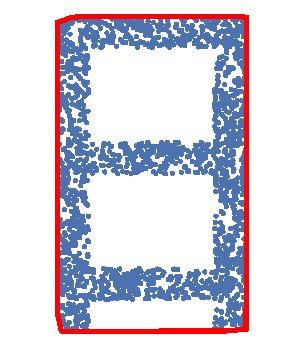
\includegraphics[width=.8\linewidth]{chapter_3_polylidar3d/imgs/concave_vs_convex_lettera_1.pdf}
    \caption{\label{fig:ch3_convex_concave_2}Convex}\vspace{6pt}
  \end{subfigure}
  \begin{subfigure}{.24\linewidth}
    \centering
\includegraphics[width=.8\linewidth]{chapter_3_polylidar3d/imgs/concave_vs_convex_lettera_2.pdf}
    \caption{\label{fig:ch3_convex_concave_3}Non-convex}\vspace{6pt}
  \end{subfigure}
  \begin{subfigure}{.24\linewidth}
    \centering
\includegraphics[width=.8\linewidth]{chapter_3_polylidar3d/imgs/concave_vs_convex_lettera_3.pdf}
    \caption{\label{fig:ch3_convex_concave_4}Non-convex with~holes}\vspace{6pt}
  \end{subfigure}
  \caption[Example polygons that can be generated from plane segmented point clouds]{Example polygons that can be generated from plane segmented point clouds. (\textbf{a})~2D~point set representation of a floor diagram with interior offices;  (\textbf{b})~Convex~polygon; (\textbf{c})~non-convex~polygon; (\textbf{d})~and~non-convex polygon with holes.~The~exterior hull (green) and interior holes (orange) are~indicated. }\label{fig:ch3_convex_concave}
\end{figure}


Biswas et al.~\cite{biswas_planar_2012} represents flat surfaces as convex polygons extracted from range images. First, points~are randomly sampled in the image with nearby pixel neighbors used for fast RANSAC plane fitting. This returns numerous sparse point subsets which may be coplanar.~The~convex hull is computed for each of these subsets generating many convex polygons in the scene. Polygons belonging to the same surface are then merged with \ac{GPU} accelerated correspondence matching. The~sparse random sampling of the point cloud and efficient generation of convex hulls allows the algorithm to run in real-time (less than 2 ms). However, convex hulls ignore boundary concavities, overestimate the area of the enclosed point set, and~do no not account for holes per Figure~\ref{fig:ch3_convex_concave}b. Poppinga et al.~\cite{poppinga_fast_2008} outlines a  method to convert plane segmented range images into convex polygons. 
%First, region growing is performed to generate planar segments. 
Each plane segment is decomposed into  a set of convex polygons. Each polygon is progressively built through scan-lines; a new polygon is generated when convexity constraints are not met. This allows a concave plane to be represented by multiple convex polygons. 
Lee et al.~\cite{lee_indoor_2012-1} generates non-convex polygons from range images. The~range image is first planar-segmented using an eight-way flood fill algorithm. This involves region growing which accounts for the normal vector to each point. Each of the planar segments is then converted to a non-convex polygon. Exterior boundary pixels of a plane segment are sampled and neighboring samples connected to create a non-convex polygon. However interior holes in the plane segments are not explicitly captured as shown in Figure ~\ref{fig:ch3_convex_concave}c. Trevor et al.~\cite{trevor2013efficient} performs a similar polygon extraction procedure through boundary tracing of the exterior~hull. 

Non-convex polygons with holes may be generated through a variety of methods, many under the name of concave hulls~\cite{edelsbrunner_shape_1983, furieri_spatialite_2017, open_source_geospatial_foundation_postgis_2019}. Many of these methods strictly operate on 2D data, requiring~the 3D planar point cloud segments be projected to the best fit geometric plane to produce 2D point sets. Holz et al.~\cite{lee_fast_2013} proposes this technique and the use of $\alpha$-shapes to extract such polygons~\cite{edelsbrunner_shape_1983}.  We~developed a faster open source polygon extraction algorithm, Polylidar, which extracts non-convex polygons with holes from 2D point sets~\cite{castagno_polylidar_2020}. The point set is converted to a 2D mesh through Delaunay triangulation, and~triangles are subsequently filtered by edge length creating the ``shape'' of the point set. This~filtered mesh is then converted to a polygon through boundary following while accounting for holes. Benchmarks demonstrate that our algorithm is a minimum of four times faster than leading methods~\cite{polylidar_benchmark_concave}. This chapter extends Polylidar to operate directly on 3D data, performing planar segmentation and polygon extraction in parallel. This integration allows Polylidar3D to skip expensive Delaunay triangulation previously required for organized point clouds as shown in Section ~\ref{sec:ch3_methods_mesh_opc}.  Planar segments represented as non-convex polygons with holes gives the following advantages:

\begin{enumerate}
    \item Significantly reduced memory requirements, on~the order of square root (perimeter vs area).
    \item Faster computation of geometric values of interest, e.g.,~centroid, area, perimeter.
    \item Ability to dilate, erode, and~simplify polygons through computational geometry routines.
    \item Holes inside a polygon account for gaps or obstacles on flat surfaces.
\end{enumerate}

\subsection{3D Data~Denoising}\label{sec:ch3_bg_mesh_smoothing}

% {\color{blue}Thinking of removing all the blue text. This section discusses denoising techniques for range images and triangular meshes. This is not a comprehensive review of data denoising but provides background to explain methods in Section~\ref{sec:ch3_bg_mesh_smoothing}.  Standard spatial image filters, such as mean, median, and gaussian filters, overly smooth edges for range images. Edge-preserving filters, such as the bilateral filter, can be used instead~\cite{tomasi_bilateral_1998}. However the computational demand of the bilateral filter is high because it uses a space-varying weighting function computed at a space of higher dimensionality than the signal being filtered~\cite{gastal_domain_2011}. Ref.~\cite{gastal_domain_2011} proposes a fast linear time edge-preserving filter which transforms a 2D image to 1D while preserves the geodesic distance between points on these curves.  Filtering is done in 1D space providing a significant speedup. The Intel RealSense SDK provides a modified implementation of this algorithm for fast edge-preserving spatial smoothing of range images~\cite{realsense_sdk_filter}.}

This section discusses two methods to smooth a mesh. The~Laplacian filter performs weighted averaging of nearby vertex neighbors to reduce noise~\cite{taubin_curve_1995}. Vertices are updated according to
\begin{align}
  v_o = v_i \cdot \frac{\lambda}{W} \sum_{j=1}^{N} w_j \cdot (v_i-v_j) \label{eq:ch3_laplacian_vertex}  \\
  w_j = ||v_i-v_j||^{-1} \quad \label{eq:ch3_laplacian_weight}
  W = \sum_{j=1}^{N} w_j
\end{align}
where $v_o$, $v_i$, $v_j$, and~$N$ denote the output (smoothed) vertex, input vertex, neighboring vertex, and~total number of neighbors, respectively. Weighting for each neighbor vertex $w_j$ is the inverse of its Euclidean distance and is normalized with $W$.  Parameter $\lambda$ adjusts smoothing [0-1], though~multiple iterations may be performed to increase smoothing. The~Laplacian filter is not edge-preserving. % causing rounding of sharp~edges. 

Zheng et al.~\cite{zheng_bilateral_2011} proposes a bilateral filtering technique on triangular meshes that is analogous to images.   Filtering occurs in two stages: normal smoothing and vertex updating. The~first stage performs local iterative normal filtering to smooth normals but preserves edges as given by:
\begin{align}
  n_o = K \sum_{j=1}^{N} W_c(||c_i-c_j||) \cdot W_s(||n_i-n_j||) \cdot n_j \label{eq:ch3_bilateral} \\
  W_c(||c_i-c_j||) = \operatorname{exp}(-||c_i-c_j||^2/2\sigma_c^2 ) \label{eq:ch3_bilateral_centroid} \\
  W_s(||n_i-n_j||) = \operatorname{exp}(-||n_i-n_j||^2/2\sigma_s^2 ) \label{eq:ch3_bilateral_normal}\\
  K = 1 / \sum_{j=1}^{N} W_c(||c_i-c_j||) \cdot W_s(||n_i-n_j||)
\end{align}
where $n_o$, $n_i$, $c_i$, $n_j$, $c_j$, and~$N$ denote smoothed triangle normal, input normal, centroid, neighbor normal, neighbor centroid, and~number of neighbors, respectively.~Triangle weights $W_c$ and $W_s$ exponentially decay based upon deviation from the triangle position and normal and parameters $\sigma_c$ and $\sigma_s$. Sharp edges can be preserved. Holz et al.~\cite{lee_fast_2013} performs a similar normal filtering technique but includes an optional intensity term for colored point clouds. A~second stage updates vertices using a method proposed by Sun et al.~\cite{sun_fast_2007} which executes weighted averaging of neighboring vertices using the newly smoothed normals. Note that smoothing may not be possible if a triangular mesh is so noisy that neighboring triangles have significantly different~normals. 

Both Laplacian and bilateral filtering rely upon neighboring triangles for smoothing.  The~neighbors are often limited to their 1-ring neighbors defined by vertex or edge neighbors. In~Section~\ref{sec:ch3_bg_mesh_smoothing} we provide accelerated implementations of these algorithms for use with organized point clouds. The~organized structure allows an implicit triangular mesh to be defined (i.e., no data structures is needed to store the graph) with the ability to use arbitrary kernel sizes to expand the neighorhood graph, a~necessary feature with dense noisy point clouds. 
% Single-threaded CPU, multi-threaded CPU, and GPU accelerated implementations are provided for Laplacian and bilateral filtering.


\subsection{Dominant Plane Normal~Estimation}\label{sec:ch3_bg_dominant_plane_normal}

The Gaussian accumulator (spherical histogram) is a widely used method for detecting planar surfaces ~\cite{borrmann_3d_2011}. It discretizes the surface of the unit sphere (S2) into individual cells, creating ``bins'' or ``buckets'' of a histogram. A~``vote'' for a possible plane, often in the form of unit normal and origin offset, are~accumulated into this histogram. Peak detection strategies on the histogram can then find dominant plane normals. Many discretization strategies of S2 exist with tradeoffs in speed, memory requirements, and~subsequent peak~detection.


The UV Sphere discretization strategy (Figure~\ref{fig:ch3_bg_ga}a,b) decomposes S2 into a 2D array by polar coordinates $\theta$ and $\phi$. Each dimension is discretized in equal steps creating a fixed number of cells, $n_{\theta}$~$\times$~$n_{\phi}$. A~unit normal to be integrated, $\hat{n}_i \in \mathbb{R}^3$, is converted to polar coordinates $\theta_i~\in~[0, 360],~\phi_i~\in~[0, 180]$ to identify its corresponding histogram cell in the 2D array. Finding the 2D array index requires a simple operation, e.g.,~ $\theta_{index} = \theta_i / 360^{\circ} \cdot n_{\theta}$. However UV Sphere cells have different shapes and area with very small cells at the poles resulting in three issues: unequal weighting (voting) during accumulation,  singularities at the poles, and~non-equivariant kernels for peak detection. Figure~\ref{fig:ch3_bg_ga}e~shows an example UV sphere histogram that fails to detect a plane at the top (North) pole.

Borrmann et al.~\cite{borrmann_3d_2011} and Limberger et al.~\cite{limberger_real-time_2015} recommend adjusting azimuth step size based upon elevation angle leading to more uniform cell area.  This creates a `Ball'' Sphere with strips with a varying number of cells for each elevation angle stored as a list of lists (Figure~\ref{fig:ch3_bg_ga}c,d). Cell areas are similar but have different shapes; a substantially larger cap is placed at the poles. Limberger et al.~\cite{limberger_real-time_2015} attempts to handle the singularity near the poles after peak detection through a vote weighting scheme. However any discretization strategy by polar coordinates will not have equivariant kernels during peak detection caused by anisotropic cells~\cite{cohen_gauge_2019}. 
\vspace{-6pt}
\begin{figure}[H]
\centering
  \begin{subfigure}[t]{.23\linewidth}
    \centering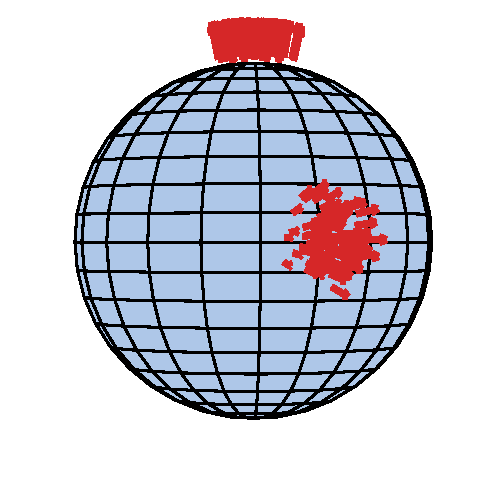
\includegraphics[width=.95\linewidth]{chapter_3_polylidar3d/imgs/ref_ga/uv_sphere_1.pdf}
    \caption{UV Sphere, Equator\label{fig:ch3_bg_ga_a}}
  \end{subfigure}
  \begin{subfigure}[t]{.23\linewidth}
    \centering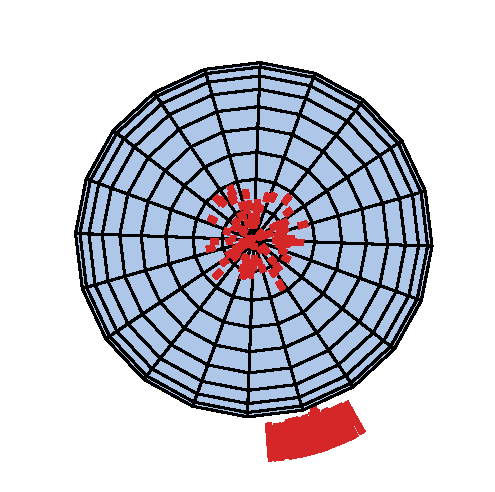
\includegraphics[width=.95\linewidth]{chapter_3_polylidar3d/imgs/ref_ga/uv_sphere_2.pdf}
    \caption{UV Sphere, Pole\label{fig:ch3_bg_ga_b}}
  \end{subfigure}
  \begin{subfigure}[t]{.23\linewidth}
    \centering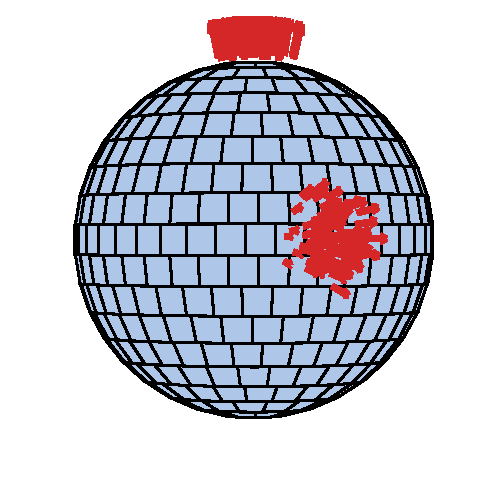
\includegraphics[width=.95\linewidth]{chapter_3_polylidar3d/imgs/ref_ga/strips_sphere_1.pdf}
    \caption{Ball Sphere, Equator\label{fig:ch3_bg_ga_c}}
  \end{subfigure}
   \begin{subfigure}[t]{.23\linewidth}
    \centering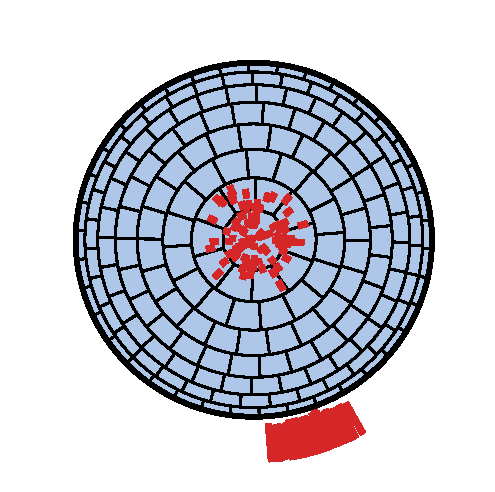
\includegraphics[width=.95\linewidth]{chapter_3_polylidar3d/imgs/ref_ga/strips_sphere_2.pdf}
    \caption{Ball Sphere, Pole\label{fig:ch3_bg_ga_d}}
  \end{subfigure}
  \par\bigskip
    \centering
  \begin{subfigure}[t]{.49\linewidth}
    \centering\includegraphics[width=.99\linewidth]{chapter_3_polylidar3d/imgs/ref_ga/uv_histogram.pdf}
    \caption{UV Sphere, Histogram\label{fig:ch3_bg_ga_e}}\vspace{6pt}
  \end{subfigure}
%   \hspace{1cm}
  \begin{subfigure}[t]{.49\linewidth}
    \centering\includegraphics[trim=0.1cm 0cm 0.99cm 0.6cm,width=.99\linewidth]{chapter_3_polylidar3d/imgs/ref_ga/strips_histogram.pdf}
    \caption{Ball Sphere, Histogram\label{fig:ch3_bg_ga_f}}\vspace{6pt}
  \end{subfigure}
  \caption[Example of integrating surface normals into Gaussian Accumulators]{Examples of integrating normals from two identically ``noisy'' planes (red arrows, Gaussian~distributed) into a UV Sphere (\textbf{a},\textbf{b}) and Ball Sphere (\textbf{c},\textbf{d}). Note the anisotropic property of sphere cells caused by unequal area and shape; (\textbf{e}) The UV Sphere histogram is unable to detect the peak at the pole; (\textbf{f}) The Ball sphere is able to detect both peaks, but~the north pole cell is significantly larger
  leading to an incorrectly higher value than the equator cell.}\label{fig:ch3_bg_ga}
\end{figure}


%The coverage area and shape of neighboring cells changes through rotations.
%This situation becomes much more apparent the finer the discretization of the sphere.
% (e.g., the cells are anisotropic because neighbors are closer and have significantly different shapes at the poles then at the equator)
% Review of accumulators
Toony et al.~\cite{toony_describing_2015} proposes unit sphere tessellation into 1996 equilateral triangle cells.~This approach gives near uniform cells in area and shape, resolving previous issues with unequal weighting, pole~singularities, and~non-equivariant kernels. The~process of integrating a unit normal into the histogram is no longer an indexing scheme. They propose to use a $K$-$D$ tree to spatially index each cell using its triangle normal.  A~nearest neighbor search must be conducted for every unit normal integrated into the histogram. Peak detection is not performed, instead the sorted histogram distribution is analyzed to predict the shape of the object being integrated (e.g., circle, plane, or~torus). 

In Polylidar3D we tessellate the unit sphere with triangles by recursively subdividing the primary faces of an icosahedron. The~recursion level dictates the approximation of the unit sphere. Our search strategy does not rely upon $K$-$D$ trees but instead uses a global index from space filling curves followed by local neighborhood search. We unfold the icosahedron into a 2D image in a particular way that guarantees equivariant kernels as outlined in~\cite{cohen_gauge_2019}. Standard 2D image peak detection is performed with nearby peaks clustered using \ac{AHC}.

% Simple Array


% Simple Array
% \cite{cao_roof_2017}

% Triangles



% Atlas of 


% \subsection{Polylidar-2d Point Sets}\label{sec:ch3_bg_poylidar}

% This needs to be in prelimaries

% Polylidar is an algorithm previously created by the authors that extracts polygons from 2D point sets~\cite{}. Polylidar is able to extract multiple disjoint polygons and capture interior holes. The algorithm proceeds in four steps:
% \begin{enumerate}
%     \item Triangulation of the Point Set
%     \item Triangle Filtering
%     \item Connected Mesh Region Extraction
%     \item Polygon Extraction
% \end{enumerate}

% The algorithm begins by first applying Delaunay triangulation to a 2D point set and filtering triangles by user configurable parameters such as triangle edge length. Afterwards, triangles which share edges are extracted into triangular mesh regions that represent the shape of the point set. Finally each region is rapidly transformed into valid concave polygon. The major contribution to Polylidar's speed is in efficiently transforming each triangular region into a concave polygon. This is done by rapidly identifying boundary edges, walking the hull of the mesh, and handling edge cases to ensure a valid polygon is returned. We encourage the readers to read the original chapter to see details of the algorithm and benchmarks~\cite{}.

% This chapter will outline our 3D extension to Polylidar where input 3D point clouds are transformed to polygons representing flat surfaces. We also present methods to filter and simplify returned polygons generated.

\section{Preliminaries}\label{sec:ch3_prelim}

A 3D point $ \vec{{p}}$ is defined in a Cartesian reference frame by orthogonal bases $\hat{\mathbf{e}}_x$,  $\hat{\mathbf{e}}_y$,  and~$\hat{\mathbf{e}}_z$:
\begin{equation}
\label{eq:ch3_point}
    \vec{{p}}=x\,\hat{\mathbf{e}}_x + y\, \hat{\mathbf{e}}_y + z\, \hat{\mathbf{e}}_z= [x,y,z]
\end{equation}

An \emph{unorganized} 3D point cloud is an arbitrarily ordered array of points denoted as $\mathcal{P}=\{ \vec{{p}_{0}}, \vec{{p}_{i}}, \ldots, \vec{{p}}_{n-1} \}$ with an index $i \in [0, n-1]$.
An \emph{organized} 3D point cloud is structured with 2D indices $u \in [0, M -1], v \in [1, N -1]$ such that $\vec{p}_{u,v} = [\vec{x}_{u,v}, \vec{y}_{u,v}, \vec{z}_{u,v}]$.   Neighboring 2D indices ($u,v$) and ($u+1, v+1$) represent 3D proximity relationships between $p_{u,v}$ and $p_{u+1,v+1}$ when they lie on the same surface~\cite{feng_fast_2014}. These 2D indices create an \emph{image space} with $M$ and $N$ denoting the rows and columns. 
%such that $n = M \cdot N$. 
Note that the 2D indices can be collapsed to a 1D stacked array by $i = u \cdot N + v$. % such that the previous definition of $\mathcal{P}$ may be used.
%  Organized point clouds can be provided by range sensors such as RGBD cameras and 3D laser scanners.
% We denote the ordered 2D  $\mathcal{OP}= \{ \vec{{p}}_{1,1}, \vec{{p}}_{1,2}, \ldots, \vec{{p}}_{2,1}, \ldots, \vec{{p}}_{M,N} \}$.
 A triangular mesh $ \mathcal{T}$ with $k$ triangles is defined by
\begin{equation}
\label{eq:ch3_tri}
    \mathcal{T} = \{ t_0, t_i, \ldots, t_{k-1} \}
\end{equation}
where each $t_i$ is a triangle with vertices defined by three point indices $\{i_0, i_1, i_2\} \in \left[0,n-1\right]$ referencing points in $\mathcal{P}$. A~half-edge triangulation further decomposes each triangle into three individual half-edges. Specifically each edge in the mesh is split into two oriented half-edges, often called twin or opposite edges~\cite{paris_modified_2013}. Each half-edge is represented by a unique id $he_j$ in triangle $t_i = \operatorname{floor}(he_j/3)$. An~ordered array $\mathcal{HE}$ is created to find corresponding twin edges. Specifically the twin edge of $he_i$ can be found at index $i$ in $\mathcal{HE}$. If~no twin exists, i.e.,~the edge is on a border, then -1 is~returned.

% A geometric plane, in point-normal form, is defined by a normal $\hat{\mathbf{n}}$ and position $\hat{p}$ 
% \begin{equation}
%     \hat{n} \cdot (\hat{r}-\hat{p}) = 0
% \end{equation}
% where $\hat{r}$ denotes any point on the plane.

% The Open Geospatial Consortium (OGC) standard~\cite{herring_opengis_2006-1} defines a \textit{linear ring} as a consecutive list of points that is both closed and simple. This mandates the linear ring to have non-intersecting line segments that join to form a closed path. A~valid \textit{polygon} must have a single exterior linear ring representing the hull of the polygon and a set of linear rings (possibly empty) representing holes inside the~polygon. 

% \section{Polylidar3d} \label{sec:ch3_methods_polylidar}

\section{Mesh~Creation}\label{sec:ch3_methods_mesh_creation}

Polylidar3D requires a half-edge triangulated mesh to perform plane and polygon extraction. Mesh generation for unorganized and organized 3D points clouds is described below, followed by details on converting a user-provided triangular mesh to half-edge~form.

\subsection{Unorganized 3D Point~Clouds}\label{sec:ch3_methods_mesh_upc}

We convert an unorganized 3D point cloud $\mathcal{P}$ into a 3D triangular mesh through 2.5D Delaunay triangulation~\cite{de_berg_delaunay_2008}. $\mathcal{P}$ is projected to the $xy$ plane, creating a corresponding 2D point set that is subsequently triangulated.  Half-edge triangulation is provided by the Delaunator library with robust geometric predicates~\cite{noauthor_github_2018, richard_shewchuk_adaptive_1997}. Although~triangulation is performed in 2D, both 2D and 3D point sets have 1:1 correspondence, allowing dual construction of the 3D mesh. Figure~\ref{fig:ch3_25DMeshCreation} demonstrates this technique applied to a synthetic rooftop scene with noisy point clouds from an overhead sensor. The~rooftop is captured at a slight angle providing points of one side of a building wall.  Only planar segments roughly aligned with $xy$ plane can be extracted with this technique, i.e.,~only the rooftop can be extracted, no walls. This type of conversion is most suitable for 3D points clouds generated from a top down viewpoint, such as airborne LiDAR point clouds as shown in Section~\ref{sec:ch3_results_rooftop}. In~this situation the plane normal to be extracted is already aligned with the $xy$ plane. 

\vspace{-6pt}

\begin{figure}[H]
\centering
  \begin{subfigure}{.48\linewidth}
    \centering\includegraphics[width=.65\linewidth]{chapter_3_polylidar3d/imgs/Basic25DAlgorithm_pointcloud.pdf}
    \caption{\label{fig:ch3_25DPoints}Unorganized 3D Point~Cloud}\vspace{6pt}
  \end{subfigure}
  \begin{subfigure}{.48\linewidth}
    \centering\includegraphics[width=.65\linewidth]{chapter_3_polylidar3d/imgs/Basic25DAlgorithm_mesh.pdf}
    \caption{\label{fig:ch3_25DMesh}2D and 3D~Mesh}\vspace{6pt}
  \end{subfigure}
  \caption[Converting an unorganized 3D point cloud to a 3D triangular mesh]{Example conversion of an unorganized 3D point cloud to a 3D triangular mesh. (\textbf{a})~Synthetic~point cloud of a  rooftop scene generated from an overhead laser scanner. A~single wall is captured because the scanner is slightly angled; (\textbf{b}) The point cloud is projected to the $xy$ plane and triangulated, generating the dual 3D mesh. Only planes aligned with the $xy$ plane can be~captured.  }\label{fig:ch3_25DMeshCreation}
\end{figure}

Plane normals may not be aligned with the inertial $xy$ plane, e.g.,~3D laser scanner rigidly mounted on an automobile. The~point cloud, generated in the sensor frame, must then be rotated such that desired plane to be extracted is aligned with $xy$ plane. This requires a priori knowledge of the plane normal and rigid body transformation necessary to align the sensor frame point cloud as demonstrated in Section~\ref{sec:ch3_results_kitti} where the ground plane (road) is extracted from point clouds generated by a spinning LiDAR sensor mounted on a~car.



\subsection{Organized 3D Point~Clouds}\label{sec:ch3_methods_mesh_opc}


Half-edge triangulation of an M $\times$ N organized point cloud can be quickly computed using spatial relationships from the image space. The triangulation is computed using neighboring image indices to define triangle vertex connections. This is in contrast to Delaunay triangulation which operates on the points themselves and maximizes the minimum angle of all the angles for each triangle in the triangulation \cite{de_berg_delaunay_2008}. Our procedure is similar to Holz et al.~\cite{lee_fast_2013} except our method creates an explicit half-edge triangulation and only uses right-cut triangles. Our half-edge triangulation allows efficient triangle region growing which is a requirement for real-time polygon extraction.  Holz et al.~\cite{lee_fast_2013} performs adaptive meshing, switching between right and left cut triangles, to~better handle missing data at the expense of increased computational demand. Figure~\ref{fig:ch3_OPC_Mesh_all} demonstrates an example conversion of a 7 $\times$ 7 organized point cloud to a half-edge mesh using our procedure. The~procedure creates the triangle set $\mathcal{T}$, half-edge array $ \mathcal{HE}$, and~a triangle map $\mathcal{T}_{map}$ as documented~below.


\vspace{-6pt}
\begin{figure}[H]
  \begin{subfigure}[t]{.33\linewidth}
    \centering\includegraphics[width=.95\linewidth]{chapter_3_polylidar3d/imgs/OPCHalfEdge-OPC-MeshV2.pdf}
    \caption{\label{fig:ch3_OPC_FC}Implicit Mesh, $\mathcal{T}_{FC}$ }\vspace{6pt}
  \end{subfigure}
  \begin{subfigure}[t]{.33\linewidth}
    % \centering\includegraphics[trim=0.1cm 1.7cm 1.0cm 0cm,width=.99\linewidth]{chapter_3_polylidar3d/imgs/OPCHalfEdge-HalfEdgeFocus.pdf}
  \centering\includegraphics[trim=0.1cm 1.7cm 1.0cm 0cm,width=.99\linewidth]{chapter_3_polylidar3d/imgs/OPCHalfEdge-HalfEdgeFocusV2.pdf}
    \caption{\label{fig:ch3_OPC_HE} Triangle indexing~scheme}\vspace{6pt}
  \end{subfigure}
  \begin{subfigure}[t]{.33\linewidth}
     \centering\includegraphics[width=.95\linewidth]{chapter_3_polylidar3d/imgs/OPCHalfEdge-OPC-Mesh_actual_V2.pdf}
    \caption{\label{fig:ch3_OPC_Mesh} Final Mesh, $\mathcal{T}$ }\vspace{6pt}
  \end{subfigure}
  \caption[Converting an organized point cloud into a 3D triangular mesh]{Example conversion of a 7 $\times$ 7 Organized Point Cloud (OPC) to a half-edge triangular mesh.~Points are represented by circles; red indicates an invalid value (e.g.,~0~depth~measurement). (\textbf{a})~Implicit~mesh of \ac{OPC} with right cut triangles, $\mathcal{T}_{FC}$.~A unique global id $GID = 2 \cdot (u \cdot (N-1) + v) + k$ is shown inside each triangle;  (\textbf{b}) Indexing scheme to define $GID$s for triangles in $\mathcal{T}_{FC}$; (\textbf{c}) Final mesh $\mathcal{T}$ with triangles created if and only if all vertices are valid. Unique indices into $\mathcal{T}$  are marked.  $\mathcal{T}_{map}$ maps between $GID$s in $\mathcal{T}_{FC}$ to $\mathcal{T}$. }\label{fig:ch3_OPC_Mesh_all}
\end{figure}
First, any invalid data in the point cloud is set to an NaN floating point value.~This keeps the point cloud organized and prompts removal of invalid triangles in the mesh.~An~implicit fully-connected right-cut mesh triangulates all points, including invalid points marked red in Figure~\ref{fig:ch3_OPC_Mesh_all}a and denoted~$\mathcal{T}_{FC}$.  Each 2 $\times$ 2 grid in the \ac{OPC} creates two triangles, which we denote first and second as shown in Figure~\ref{fig:ch3_OPC_Mesh_all}b. Each triangle in $\mathcal{T}_{FC}$ is indexed by $t_{u,v,k}$ where  $k \in \{0,1\}$ represents the first or second triangle, respectively. A~unique global id $GID = 2 \cdot (u \cdot (N-1) + v) + k$ is shown inside each triangle in Figure~\ref{fig:ch3_OPC_Mesh_all}a. This $GID$ represents the triangle order within $\mathcal{T}_{FC}$.  The~final mesh returned $\mathcal{T}$ is shown in Figure~\ref{fig:ch3_OPC_Mesh_all}c with construction outlined in Algorithm \ref{alg:ch3_opc_mesh_creation}. The~data structure $\mathcal{T}_{map}$ defines a mapping of global ids in $\mathcal{T}_{FC}$ to their index positions in $\mathcal{T}$ (if they exist, else  $-$1) which is used later in half-edge extraction. Algorithm \ref{alg:ch3_opc_mesh_creation} begins by iterating over all 2 $\times$ 2 point grids and constructs the first and second triangle for each. These respective triangles are only added to $\mathcal{T}$ if all three points are valid. Triangle point indices are added counter-clockwise with the three half-edges implicitly defined by the ordered traversal of point indices, e.g.,~the first triangle's half-edges are [PI3 $\rightarrow$ PI2, PI2 $\rightarrow$ PI1, PI1 $\rightarrow$ PI3]. 


% Note that $\mathcal{T}_{FC}$ is never actually created, it only exists as a construct to give neighboring relationships between triangles and provide global id's (GID) to every possible triangle. 
% $u \in [0, M-2]]$, $v \in [0, N-2]]$, and



% Neighboring relationships are fixed for every triangle such that $GID$s are computed

% l that $\mathcal{HE}$ is a flat array indexed by half-edge ID which provides its twin/opposite half-edge ID or -1 if none exists. As before we loop through every 2X2 grid, examining the first and second triangles formed. The first, second, top, right, bottom, and left triangles IDs are determined by mapping $\mathcal{T}_{FC}$ $GID$s with $\mathcal{T}_{map}$.  If these triangles are in $\mathcal{T}$, determined by checking for a  sentinel value in $\mathcal{T}_{map}$, their associated half-edges are mapped to the correct shared half-edge in $\mathcal{HE}$. 
%Note that Algorithm \ref{alg:ch3_opc_halfedge_creation} is simplified 

% \vspace{6pt}

% \begin{singlespace}
\begin{algorithm}[H]
    \SetKwInOut{Input}{Input}
    \SetKwInOut{Output}{Output}
    \SetStartEndCondition{ }{}{}%
    \SetKwProg{Fn}{def}{\string:}{}
    % \SetKwFunction{Range}{range}%%
    % \SetKw{KwTo}{in}\SetKwFor{For}{for}{\string:}{}%
    \SetKwIF{If}{ElseIf}{Else}{if}{:}{elif}{else:}{}%
    % \SetKwFor{While}{while}{:}{fintq}%
    % \AlgoDontDisplayBlockMarkers\SetAlgoNoEnd\SetAlgoNoLine%

    \Input{Organized Point Cloud: $\mathcal{P}$ \\ 
           Rows: M, Columns: N }
    \Output{Triangle Set: $\mathcal{T}$ \\
           Triangle Map: $\mathcal{T}_{map}$}
    $N' = N-1$, 
    $M' = M-1$ \\
    $\mathcal{T} = \emptyset$ \\
    $SV = -1 $ \tcc*[h]{Sentinel Value indicating invalid triangle} \\
    $\mathcal{T}_{map} = [SV, SV, \ldots, SV]$ \tcc*[h]{$|T_{map}| = 2 \cdot M' \cdot N' $} \\
    $n_{tri}$ = 0 \\
    \For{$u \leftarrow 0$ \KwTo  $M'-1$ \hspace{.1cm} }{
        \For{$v \leftarrow 0$ \KwTo  $N'-1$ \hspace{.1cm} }{
            $First_{GID} = 2 \cdot (u \cdot N' + v)$, 
            $Second_{GID} = 2 \cdot (u \cdot N' + v) + 1$ \\
            p1, p2, p3, p4 = GetPointIndices(u, v)\\
            \tcc{First Triangle}
            \uIf{$\operatorname{NotNan}$(p1, p2, p3, $\mathcal{P}$) }{
                $\mathcal{T}$ = $\mathcal{T}$ + \{ p3, p2, p1 \} \\
                $\mathcal{T}_{map}[First_{GID}] =  n_{tri}$ \\
                $n_{tri} = n_{tri} + 1$ \\
            }
            \tcc{Second Triangle}
            \uIf{$\operatorname{NotNan}$(p1, p3, p4, $\mathcal{P}$) }{
                $\mathcal{T}$ = $\mathcal{T}$ + \{ p1, p4, p3 \} \\
                $\mathcal{T}_{map}[Second_{GID}] =  n_{tri}$ \\
                $n_{tri} = n_{tri} + 1$ \\
            }
        }
    }
    return $\mathcal{T}, \mathcal{T}_{map}$
    \caption{Extract Triangles from~\ac{OPC}}
    \label{alg:ch3_opc_mesh_creation}
\end{algorithm}
% \end{singlespace}
% \vspace{6pt}
The half-edge array $\mathcal{HE}$ is constructed 
%in Algorithm \ref{alg:ch3_opc_halfedge_creation}
using the previously calculated $\mathcal{T}_{map}$ and is shown in Algorithm \ref{alg:ch3_opc_halfedge_creation}. The~algorithm begins at Line 3 by setting all half-edges in $\mathcal{HE}$ to the default sentinel value of $-$1 indicating no shared edge.  Line 4 and 5 then begin iterating through every 2 $\times$ 2 grid in the \ac{OPC} inspecting the first and second triangles in $\mathcal{T}_{FC}$. Line 6 and 7 retrieve the index of these triangles in $\mathcal{T}$ using $\mathcal{T}_{map}$ if they exist. If~these triangles exist then their neighboring triangles may be assigned in Lines 9 and 18, respectively. For~example in Line 13 if the right triangle neighbor exists then its first edge corresponding to a half-edge id of $3 \cdot Right_{idx}$ will be linked to the first half-edge of the first~triangle.

% \begin{singlespace}
\begin{algorithm}[H]
    \SetKwInOut{Input}{Input}
    \SetKwInOut{Output}{Output}
    \SetStartEndCondition{ }{}{}%
    \SetKwProg{Fn}{def}{\string:}{}
    % \SetKwFunction{Range}{range}%%
    % \SetKw{KwTo}{in}\SetKwFor{For}{for}{\string:}{}%
    \SetKwIF{If}{ElseIf}{Else}{if}{:}{elif}{else:}{}%
    % \SetKwFor{While}{while}{:}{fintq}%
    % \AlgoDontDisplayBlockMarkers\SetAlgoNoEnd\SetAlgoNoLine%

    \Input{Triangle Map: $\mathcal{T}_{map}$ \\ 
          Rows: M, Columns: N }
    \Output{Half-Edge Set: $\mathcal{HE}$}
    $N' = N-1$, 
    $M' = M-1$ \\
    $SV = -1$ \tcc*[h]{Sentinel value indicating no shared edge } \\
    $\mathcal{HE} = [SV, SV, \ldots, SV]$ \tcc*[h]{$|\mathcal{HE}| = 3 \cdot |\mathcal{T}| $} \\
    \For{$u \leftarrow 0$ \KwTo  $M'-1$ \hspace{.1cm} }{
        \For{$v \leftarrow 0$ \KwTo  $N'-1$ \hspace{.1cm} }{
            $First_{idx}$ = $\mathcal{T}_{map}[2 \cdot (u \cdot N' + v)] $\\
            $Second_{idx}$ = $\mathcal{T}_{map}[2 \cdot (u \cdot N' + v) + 1] $\\
            $Top_{GID}$, $Right_{GID}$, $Bottom_{GID}$, $Left_{GID}$ = GetNeighborsGID(u,v)\\
            \uIf{$First_{idx}$ != $SV$ }{
                $Top_{idx}$ = $\mathcal{T}_{map}[Top_{GID}] $\\
                $Right_{idx}$ = $\mathcal{T}_{map}[Right_{GID}] $\\

                \uIf{$Right_{idx}$ != $SV$ }{
                    $\mathcal{HE}[First_{idx} \cdot 3]$ = $Right_{idx} \cdot 3$
                }
                \uIf{$Top_{idx}$ != $SV$ }{
                    $\mathcal{HE}[First_{idx} \cdot 3 + 1]$ = $Top_{idx}$ $\cdot 3 + 1$
                }
                \uIf{$Second_{idx}$ != $SV$ }{
                    $\mathcal{HE}[First_{idx} \cdot 3 + 2]$ = $Second_{idx}$ $\cdot 3 + 2$
                }
            }
            \uIf{$Second_{idx}$ != $SV$ }{
                $Bottom_{idx}$ = $\mathcal{T}_{map}[Bottom_{GID}] $\\
                $Left_{idx}$ = $\mathcal{T}_{map}[Left_{GID}] $\\

                \uIf{$Left_{idx}$ != $SV$ }{
                    $\mathcal{HE}[Second_{idx} \cdot 3]$ = $Left_{idx}$ $\cdot 3$
                }
                \uIf{$Bottom_{idx}$ != $SV$ }{
                    $\mathcal{HE}[Second_{idx} \cdot 3 + 1]$ = $Bottom_{idx}$ $\cdot 3 + 1$
                }
                \uIf{$First_{idx}$ != $SV$ }{
                    $\mathcal{HE}[Second_{idx} \cdot 3 + 2]$ = $First_{idx}$ $\cdot 3 + 2$
                }
            }
        }
    }
    return $\mathcal{T}, \mathcal{T}_{map}$
    \caption{Extract Half-Edges from~\ac{OPC}}
    \label{alg:ch3_opc_halfedge_creation}
\end{algorithm}
% \end{singlespace}


\subsection{User Provided~Meshes}\label{sec:ch3_methods_mesh_user}

We define a user-provided triangle mesh as a triangle set $\mathcal{T}$ with a corresponding 3D point cloud $\mathcal{P}$. These meshes can be generated from 3D data using a variety of methods~\cite{kazhdan_screened_2013,bernardini_ball-pivoting_1999,zhou_dense_2013}. The~front-end of Polylidar3D  creates the half-edge set $\mathcal{HE}$ of this mesh to determine shared edges in similar manner to \cite{zhou_open3d_2018}. This entails first constructing half-edge hashmaps where the key is each half-edge's ordered point indices and value its half-edge ID. Opposite half-edges for any half-edge can then be found by reversing the order of its point indices and performing a hashmap lookup. If~a shared half-edge is found then its half-edge ID is mapped into $\mathcal{HE}$.

Certain forms of non-manifold meshes must be explicitly handled. We focus on a subclass of meshes that are not two-manifold. First we define two key properties of a two-manifold~mesh: 
\begin{enumerate}
    \item Every vertex connects to a single edge-connected set of triangles.
    \item Every edge is shared by one or two triangles.
\end{enumerate}

Figure~\ref{fig:ch3_NonMainifoldCond1} shows examples of non-manifold meshes where condition (1) is violated. Polylidar3D~handles violations of (1)  using methods from our previous work~\cite{castagno_polylidar_2020}. The~missing triangles (shown as white) are explicitly captured as holes inside a polygon for Figure {\ref{fig:ch3_NonMainifoldCond1}}a--c, while the mesh is split into two polygons for Figure~\ref{fig:ch3_NonMainifoldCond1}d. Figure~\ref{fig:ch3_NonMainifoldCond2} shows cases of non-manifold meshes that violate condition (2). No~mesh generated per Sections~\ref{sec:ch3_methods_mesh_upc} and \ref{sec:ch3_methods_mesh_opc} will violate (2)  because triangulation occurs in 2D space so all edges share at most two triangles. However a user-provided 3D mesh may not satisfy condition (2).


The half-edge array $\mathcal{HE}$ used for neighbor expansion during planar segment extraction in Section~\ref{sec:ch3_methods_polylidar_plane_extraction} only maps twin half-edges, making condition (2) mesh violations problematic. Three~options can handle cases when more than two shared edges exist:

\begin{enumerate}
    \item Store only the first pair of edges found and ignore any others.
    \item Select the pair of edges that are most similar. Similarity between edges is defined by comparing angular distance of their owning triangle normals. 
    \item Ignore all of them by labelling all as boundary edges.
\end{enumerate}


\begin{figure}[ht]
\centering
  \begin{subfigure}{.24\linewidth}
    \centering\includegraphics[width=.9\linewidth]{chapter_3_polylidar3d/imgs/OPCHalfEdge-ManifoldMeshA.pdf}
    \caption{\label{fig:ch3_NonMainifoldCond1A}}\vspace{6pt}
  \end{subfigure}
  \begin{subfigure}{.24\linewidth}
    \centering\includegraphics[width=.9\linewidth]{chapter_3_polylidar3d/imgs/OPCHalfEdge-ManifoldMeshB.pdf}
    \caption{\label{fig:ch3_NonMainifoldCond1B}}\vspace{6pt}
  \end{subfigure}
  \begin{subfigure}{.24\linewidth}
    \centering\includegraphics[width=.9\linewidth]{chapter_3_polylidar3d/imgs/OPCHalfEdge-ManifoldMeshC.pdf}
    \caption{\label{fig:ch3_NonMainifoldCond1C}}\vspace{6pt}
  \end{subfigure}
  \begin{subfigure}{.24\linewidth}
    \centering\includegraphics[width=.9\linewidth]{chapter_3_polylidar3d/imgs/OPCHalfEdge-ManifoldMeshD.pdf}
    \caption{\label{fig:ch3_NonMainifoldCond1D}}\vspace{6pt}
  \end{subfigure}
  \caption[Example non-manifold meshes with condition one violations]{Example non-manifold meshes that exhibit condition (1) violations. Red vertices specifically show examples where the vertex triangle set is not fully edge-connected. (\textbf{a}--\textbf{c}) will extract any missing triangles as holes from the blue triangular segment;  (\textbf{d}) The missing triangles in this mesh also cause condition (1) violations but will \emph{not} be captured as holes. They cause the green and blue portion of the mesh to not be edge-connected for region growing in Section~\ref{sec:ch3_methods_polylidar_plane_extraction}. They will be extracted as two separate segments with no holes in their respective interiors}. \label{fig:ch3_NonMainifoldCond1}
\end{figure}

\vspace{-6pt}

Option one is advantageous in speed and will generally have minimal consequences in the event an incorrect half-edge pairing is chosen, e.g.,~a green and orange triangle edge are linked in Figure~\ref{fig:ch3_NonMainifoldCond2}. If~green and orange triangle normals are sufficiently different then planar segment extraction will not connect them. However there is no guarantee that this may occur and may fail as in (Figure~\ref{fig:ch3_NonMainifoldCond2}c). Option~two attempts to remove the issue entirely by connecting only the pair of edges that are most similar (edges shared by green triangles). This technique will work for (Figure~\ref{fig:ch3_NonMainifoldCond2}a,b) but will fail once again on (Figure~\ref{fig:ch3_NonMainifoldCond2}c). Finally option three is the safest, it links none of the shared edges and treats them as border edges (edges sharing no neighbor).  This keeps the critical invariant that no condition (2)~violation will exist in an extracted planar mesh. However superfluous border edges will exist which can be handled downstream. Currently only option (1) is implemented in Polylidar3D~\cite{Castagno_Github_Polylidar} with future plans to allow the user to choose between any of the three proposed~solutions. 

% The actual process of creating the half-edge array $\mathcal{HE}$ from user provided meshes is similar to \cite {zhou2018open3d}. This entails first constructing half-edge hashmaps where the key is each half-edges ordered point indices and value its half-edge id. Opposite half-edges for any half-edge can then be found by reversing the order of its point indices and performing a lookup in the hashmap.

\vspace{-12pt}
\begin{figure}[H]
  \begin{subfigure}{.30\linewidth}
    \centering\includegraphics[clip,trim=1.1cm 5.1cm 7.1cm 5.1cm, width=.95\linewidth]{chapter_3_polylidar3d/imgs/manifold3d_one.pdf}
    \caption{Three shared~edges\label{fig:ch3_NonMainifoldCond2A}}\vspace{6pt}
  \end{subfigure}
  \begin{subfigure}{.30\linewidth}
    \centering\includegraphics[clip,trim=1.1cm 5.1cm 7.1cm 5.1cm,width=.95\linewidth]{chapter_3_polylidar3d/imgs/manifold3d_two.pdf}
    \caption{Five shared~edges\label{fig:ch3_NonMainifoldCond2B}}\vspace{6pt}
  \end{subfigure}
  \begin{subfigure}{.30\linewidth}
    \centering\includegraphics[clip,trim=1.1cm 5.1cm 9.1cm 5.1cm,width=.95\linewidth]{chapter_3_polylidar3d/imgs/manifold3d_three.pdf}
    \caption{Three shared~edges\label{fig:ch3_NonMainifoldCond2C}}\vspace{6pt}
  \end{subfigure}
  \caption[Example non-manifold meshes with condition two violations]{Examples of non-manifold meshes where an edge is shared by more than two triangles. This~common edge is shared by green and orange triangles. The~green triangles form a two-manifold mesh with the blue triangles while the orange triangle(s) do not. The~orange triangles in (Figure~\ref{fig:ch3_NonMainifoldCond2}a,b) have sufficiently different normals such the green triangles half-edges can be easily linked. However~all triangles in (Figure~\ref{fig:ch3_NonMainifoldCond2}c) have nearly equal normals making this~impossible.}\label{fig:ch3_NonMainifoldCond2}
\end{figure}
\unskip




\section{Mesh~Smoothing}\label{sec:ch3_methods_mesh_smoothing}

Mesh smoothing for user-provided triangular meshes is performed using Intel Open3D smoothing procedures~\cite{zhou_open3d_2018}.  The~sections below describe our implementation of Laplacian and bilateral filtering for the organized point cloud meshes created in Section~\ref{sec:ch3_methods_mesh_opc}.  Our implementation is open source and provides single-threaded CPU, multi-threaded CPU, and~GPU accelerated routines~\cite{Castagno_Github_opf}. 

\subsection{Laplacian~Filter}\label{sec:ch3_methods_mesh_smoothing_laplacian}

We implement the standard Laplacian filter for organized point clouds with the benefit that no explicit triangular mesh is required, only the point cloud itself. The~filtering, as~described in Equation~(\ref{eq:ch3_laplacian_vertex}), results in smoothed vertices of the mesh, i.e, the~point cloud is denoised. Vertex~neighborhood information is defined implicitly by the image space indices of the organized point cloud.  The~neighborhood size is configured by adjusting the kernel size of the filter, e.g, a~kernel size of three implies eight vertex neighbors. Filtering this way offers the following benefits:

\begin{enumerate}
    \item Neighboring vertices do not need to be found through lookup over $\mathcal{T}$, $\mathcal{HE}$, or~an adjacency list. 
    \item Neighborhood size can be increased by adjusting filter kernel-size. Increasing the kernel size is critical for extremely dense and noisy point clouds.
    \item Parallelization is trivial, similar to image filters, with~all necessary neighborhood data for a vertex located close in memory.
\end{enumerate}

The amount of filtering is controlled by $\lambda$, the~kernel size, and~the number of iterations. As~kernel size and number of iterations increase the computational demand of the filter also increases. Mesh~borders in image space have no defined neighbors on the exterior thus are not filtered. This gives a negative drawback of a noisy border but a positive benefit of reducing the mesh shrinkage inherit to Laplacian filtering. One may think of the fixed border as ``pinning'' the mesh to prevent~overshrinkage. 


\subsection{Bilateral~Filter}\label{sec:ch3_methods_mesh_smoothing_bilateral}

We implement the bilateral mesh filtering algorithm presented by Zheng et al.~\cite{zheng_bilateral_2011} but for organized point~clouds.~Smoothing occurs on the implicit fully-connected organized mesh $\mathcal{T}_{FC}$, described~in~Section~\ref{sec:ch3_methods_mesh_opc}.  Recall the mesh spatial structure is defined through image indices ($u,v$) with a final index $k \in \{0,1\}$ representing the first or second triangle in a 2 $\times$ 2 quad (see~Figure~\ref{fig:ch3_OPC_HE}). Bilateral filtering per Equation~(\ref{eq:ch3_bilateral}) requires data structures for each triangle's centroid and normal, which we denote as $\mathcal{C}$ and $\mathcal{N}$. These are constructed in parallel (if multi-core CPU is available) and laid out in contiguous memory with the same indexing scheme as $\mathcal{T}_{FC}$, i.e.,~the centroid of triangle $t_{u,v,k}$ is $c_{u,v,k}$. If~any of the vertices of a triangle in $\mathcal{T}_{FC}$  are NaN then the associated centroid and normal will also be~NaN.

The algorithm partitions triangle smoothing in image space coordinates, smoothing both the first and second triangles as one unit of work. Each triangle's normal is updated using centroid and normal information from neighboring triangles. The~neighbors of a triangle are determined by a user-configurable kernel size as shown in Figure~\ref{fig:ch3_smooth_bilateral}.  Note that defining neighbors in this way mixes both $n$-ring and $(n+1)$-ring triangle neighbors. However the exponential decay of the bilateral filter in Equations~\ref{eq:ch3_bilateral_centroid} and \ref{eq:ch3_bilateral_normal} ensures that only triangles of similar properties (close in position and orientation) will be integrated into the smoothed normal. Neighbors are not integrated if they have NaN values for their centroid/normal. The~end result is smoothed normals for $\mathcal{T}_{FC}$; however, what is actually desired are smoothed normals for $\mathcal{T}$ per Figure~\ref{fig:ch3_OPC_Mesh}. This is quickly achieved by using $\mathcal{T}_{map}$ to identify the valid normals for $\mathcal{T}$. Zheng et al.~\cite{zheng_bilateral_2011} follows up with vertex updating, but~we do not perform this step. Vertex updating is an expensive operation which provides minimal benefit for triangle region growing downstream. Only the smoothed normals are needed in~Polylidar3D. 


\begin{figure}[H]
    \centering
    \includegraphics[width=.60\linewidth]{chapter_3_polylidar3d/imgs/OPCHalfEdge-BilateralFilter.pdf}
    \caption[Visualization of a triangle's neighborhood during bilateral filtering]{Visualization of a triangle's neighborhood during bilateral filtering of an organized point~cloud.  Each 2 $\times$ 2 point group forms two triangles creating a mesh. Each triangle's neighbors are defined by the kernel size. For~example a kernel size of five includes all blue and red~triangles.}
    \label{fig:ch3_smooth_bilateral}
\end{figure}

The advantage of implementing bilateral smoothing in this manner is that all information is laid out in contiguous memory to increase cache locality. These are important characteristic for CPU and especially GPU performance. However nontrivial excess work is performed if most of the point cloud is invalid, e.g, invalid depth measurements in a range image. The~entire procedure is controlled by $\sigma_c^2$, $\sigma_s^2$, kernel size, and~number of~iterations.

\section{Dominant Plane Normal~Estimation}\label{sec:ch3_methods_fastga}

We present a new method for constructing and using a Gaussian Accumulator to identify dominant plane normals in a scene. We call this method the Fast Gaussian Accumulator (FastGA). The~input to this method is a list of $k$ unit normals $\mathcal{N} = \{\hat{n}_0, \ldots, \hat{n}_{k-1} \}$ which have been sampled from a scene. Use of denoised data is advantageous but not required. Sections~\ref{sec:ch3_methods_fastga_histogram} and \ref{sec:ch3_methods_fastga_peak} discuss constructing the Gaussian Accumulator and performing peak detection, respectively. 

\subsection{Gaussian~Accumulator}\label{sec:ch3_methods_fastga_histogram}

The following subsections describe the process to approximate a sphere using an icosahedron, construct the Gaussian Accumulator, and~our method to integrate information into the~accumulator. 

\subsubsection{Refined~Icosahedron}\label{sec:ch3_methods_fastga_ico}

A geodesic polyhedron is first constructed by using an icosahedron as the base model approximation of a unit sphere. The~icosahedron is composed of 12 vertices and 20 faces and can be seen on the far left in Figure~\ref{fig:ch3_fastga_refinement}. This polyhedron is refined by recursively dividing each face into four equilateral triangles and then projecting the new vertices onto the surface of a sphere. The~number of iterations or levels of recursion is user configurable with higher levels better approximating a sphere. The~Class I geodesic polyhedron is defined with the Schläfli symbol $\{3,5+\}_{1,0}$ with frequency doubling at each level~\cite{wenninger_spherical_1999}. Figure~\ref{fig:ch3_fastga_refinement} shows refinement up to level four while Table~\ref{table:ch3_fastga_refinement} displays the change in number of vertices, triangles, and~approximate angular separation between each triangle. We denote each triangle as the cell or bucket of the histogram of S2. The~number of cells, $n$, and~their properties described below are  fixed once a refinement level is~chosen.

\begin{figure}[H]
    \centering
    \includegraphics[width=.60\linewidth]{chapter_3_polylidar3d/imgs/fastga_ico_refinement_v2.png}
    \caption[Approximation of the unit sphere with an icosahedron]{Approximation of the unit sphere with an icosahedron. The~level 0 icosahedron is shown on the  left with increasing refinements to the right.  Triangle cells become buckets of a histogram on~S2. }
    \label{fig:ch3_fastga_refinement}
\end{figure}
\unskip

\begin{table}[H]
\centering
\caption{Levels of Refinement for an~Icosahedron.}\label{table:ch3_fastga_refinement}
\begin{tabular}{@{}cccc@{}}
\toprule
\textbf{Level} & \textbf{\# Vertices} & \textbf{\# Triangles }& \textbf{Separation} \\ \midrule
0     & 12          & 20           & $41.8^{\circ}$          \\
1     & 42          & 80           & $18.0^{\circ}$            \\
2     & 162         & 320          & $6.9^{\circ}$              \\
3     & 642         & 1280         & $3.1^{\circ}$              \\
4     & 2562        & 5120         & $1.5^{\circ}$              \\ \bottomrule
\end{tabular}
\end{table}
\unskip



\subsubsection{Gaussian Accumulator~Properties}\label{sec:ch3_methods_fastga_ga}

A space-filling curve (SFC) maps a multi‐dimensional space into a one‐dimensional space, e.g.,~$\mathcal{R}^2 \rightarrow \mathcal{R}$.  Hilbert curves are a widely used SFC because they preserve locality well during transformation~\cite{mokbel_space-filling_2008}. This means that points close in 1-D space are close in $N$-D, though~the converse is not guaranteed to be true. In~practice a SFC is approximated using discrete integers. The~S2 Geometry library~\cite{google_s2_2020} provides a SFC routine that transforms any real-valued unit normal $\hat{n}_i \in \mathcal{R}^3$ to a 64 bit unsigned integer. The~method works by projecting the unit sphere to a cube, creating 2D $\rightarrow$ 1D Hilbert curves for each of the six faces, and~finally stitching them together to make one unbroken linear chain.  Each cell in the refined icosahedron has a surface normal $\hat{n}^{c}_{i}$ that can be mapped to a unique ID denoted $s2id$ using this procedure. This generates a one-dimensional thread that passes through every cell such that each cell is visited exactly once as seen in Figure~\ref{fig:ch3_fastga_hilbert}.

\begin{figure}[H]
    \centering
    \includegraphics[width=.20\linewidth]{chapter_3_polylidar3d/imgs/fastga_ico_hilbert_v3.png}
    \caption[Space filling curve (SFC) of a level four refined icosahedron]{Space filling curve (SFC) of a level 4 icosahedron generated using the S2 Geometry Library. Each cell's surface normal is mapped to an integer creating a linear ordering for a curve. The~curve is colored according to this mapping and traverses each~cell.   }
    \label{fig:ch3_fastga_hilbert}
\end{figure}

The final Gaussian Accumulator (GA) is then an ordered array of $Cells = [ c_i, \ldots, c_{n-1}] $. Each~cell contains its surface normal $\hat{n}^{c}_{i}$, unique $s2id_i$, and~an accumulating integer $count_i$. The~cell array is sorted by $s2id$, creating the invariant that cells close together in the array are close in physical space. A~neighborhood data structure $Nbrs_{i,j}$ is constructed as an N$\times$12 matrix in which the $i^{th}$ row contains the 12 neighboring cell indices of the $i^{th}$ cell in the $Cells$ array. Neighboring triangles are defined as those in the 1-ring vertex adjacency. A~maximum of 60 triangles at any level of refinement have only 11 neighbors; all others have 12. For~these cells the $12^{th}$ neighbor index is given a sentinel value of $-$1 to indicate no neighbor is present. 
% Once again, all of this data is fixed once the level of refinement is chosen (e.g., compile time).

\subsubsection{Integrating the Gaussian Accumulator With~Search}\label{sec:ch3_methods_fastga_search}
Integrating a list of $k$ unit normals $\mathcal{N} = \{\hat{n}_0, \ldots, \hat{n}_{k-1} \}$ into the Gaussian Accumulator is done through a search that finds the corresponding cell whose surface normal is closest to an input normal $\hat{n}_i$ then incrementing the cell's $count_i$ member.
%i.e., $ c_{j^*} = \argminA_{ c_j \; \in \; Cells}\; || \hat{n}_i-\hat{n}^{c}_j ||$.
Instead of a $K$-$D$ tree search we propose combining a sorted integer search with a local neighborhood search. Though~similar, there are nontrivial differences and optimizations that make our method faster.  The~main components of the search are as follows: map $\hat{n}_i$ to an integer $s2id$, perform sorted integer interpolation search to reduce search bounds, perform~branchless binary search within these bounds in the $Cells$ array, then  perform local neighborhood search to find the correct cell. Algorithm \ref{alg:ch3_find_cell_index} outlines this search routine and is explained~below.

There exist several methods for sorted integer search such as interpolation and binary search. Interpolation search works by predicting the index of a value in a sorted array by interpolating  between the first and last value of the sorted array (thus computing a slope). The~process continues iteratively, each time reducing the search window and recomputing a new line for improved prediction. Interpolation search is best used for linear data but still often underperforms in comparison to binary search in practice due to its use of repeated computationally expensive calculations of slope~\cite{van_sandt_efficiently_2019}.

% Interpolation search has superior average asymptotic complexity in comparison to binary search,  $\mathcal{O}(\log{} \log{} n)$ vs  $\mathcal{O}(\log{}n)$ respectively. However interpolation search has a worst case complexity of $\mathcal{O}(n)$  when the integers are exponentially distributed, meaning interpolation should not be used with non-linear data.  Additionally, interpolation search often underperforms in comparison to binary search in practice due to its use of repeated computationally expensive calculations of slope~\cite{van_sandt_efficiently_2019}.

% \begin{singlespace}
\begin{algorithm}[ht]
    \SetKwInOut{Input}{Input}
    \SetKwInOut{Output}{Output}
    \SetStartEndCondition{ }{}{}%
    \SetKwProg{Fn}{def}{\string:}{}
    % \SetKwFunction{Range}{range}%%
    \SetKw{KwIs}{is}{}
    \SetKwIF{If}{ElseIf}{Else}{if}{:}{elif}{else:}{}%
    % \SetKwFor{While}{while}{:}{fintq}%
    % \AlgoDontDisplayBlockMarkers\SetAlgoNoEnd\SetAlgoNoLine%

    \Input{Unit Normal: $\hat{n}_i \in \mathcal{R}^3$ \\
           Cells Array: $Cells$ \\
           Neighbor Matrix: $Nbrs$
        %   Linear Slope: $m$  \\
        %   Linear Intercept: $b$
           
        }
    \Output{Cell Index: $k_{best} \in [0, |Cells|]$}
    
    $s2id = \operatorname{GetS2ID}(\hat{n}_i)$ \\
    $[k_{min}, k_{max}] = \operatorname{SearchWindow}(s2id) $\\
    \tcc{get closest neighbor by s2id}
    $k' = \operatorname{BranchlessBinarySearch}(s2id, Cells, k_{min}, k_{max})$\\
    $k_{best} = k'$\\
    $dist_{best} = ||\hat{n}^c_{k'}-\hat{n}_i  ||$ \\
    \tcc{local neighbor search by actual distance}
    \For{$j \leftarrow 0$ \KwTo  $12$ \hspace{.1cm} }{
       $k_{nbr} = Nbrs_{k',j}$ \\
        \uIf{$k_{nbr}$ \KwIs $-1$ }{
            continue
        }
       $dist = || \hat{n}^c_{k_{nbr}}-\hat{n}_i ||$ \\
        \uIf{$dist < dist_{best}$ }{
            $k_{best} = k_{nbr}$\\
            $dist_{best} = dist$
        }
    }
    return $k_{best}$
    \caption{Find Cell~Index}
    \label{alg:ch3_find_cell_index}
\end{algorithm}
% \end{singlespace}
% \vspace{6pt}
Figure~\ref{fig:ch3_linear_interp}a shows a graph of cells in the Gaussian Accumulator where the $x$-axis is the $s2id$ and the $y$-axis is the corresponding index into the sorted $Cells$ array. %To be clear the domain is in the range $[0, 2^{64} -1]$ and the range is $[0, n]$ where n is the number of cells in the Gaussian Accumulator. 
We use least squares regression to fit a line to the data shown in Figure~\ref{fig:ch3_linear_interp}a, in~contrast to only using the first and last values typical of interpolation search. Figure~\ref{fig:ch3_linear_interp}a shows this regressed line (green) accurately fits the data overall. In~a zoomed plot (Figure \ref{fig:ch3_linear_interp}b), model error, the~difference between actual and predicted cell array index, is~shown as the red line with values on the right vertical axis. Since the model/data domain and range are ordered and finite we can compute the negative and positive error bounds which is fixed once the GA refinement level is chosen. This is significant because one can reliably predict the correct index position of a cell with small known error bounds. This means that one does not need to perform a full binary search through the array of histogram cells but only a small subset of it. For~example, refinement level four with 5120 histogram cells has maximal error bounds of $-$16 and +16 from any predicted position, thereby reducing the search from 5120 to 32 cells. This technique brings the benefits of linear interpolation search without excess computational overhead because the model can be computed at compile~time.
\vspace{-6pt}
\begin{figure}[H]
        \centering
%   \begin{subfigure}[t]{.30\linewidth}
%     \centering\includegraphics[clip,trim=0.9cm 0cm 0.5cm 0cm, width=\linewidth]{chapter_3_polylidar3d/imgs/ga_linear_interp_0.pdf}
%         % \begin{adjustbox}{width=\linewidth} % rescale box
%     % \include{chapter_3_polylidar3d/imgs/tex/ga_linear_interp_0}
%         % \end{adjustbox} 
%     \caption{\label{fig:ch3_linear_interp_0}}
%   \end{subfigure}
%   \hfill
  \begin{subfigure}[t]{.30\linewidth}
    \centering\includegraphics[clip,trim=0.0cm 0cm 0.0cm 0cm,width=\linewidth]{chapter_3_polylidar3d/imgs/ga_linear_interp_1.pdf}
    \caption{\label{fig:ch3_linear_interp_1}}
  \end{subfigure}
\quad \quad
%   \hfill
  \begin{subfigure}[t]{.35\linewidth}
    \centering
    \includegraphics[width=\linewidth]{chapter_3_polylidar3d/imgs/ga_linear_interp_2.pdf}
    \caption{\label{fig:ch3_linear_interp_2}}
  \end{subfigure}
  \caption[Linear prediction model for space filling curve indices on a Gaussian Accumulator]{Linear prediction model for a level four Gaussian Accumulator (GA). The~5120 GA cells are sorted in an array ($Cells$) by their corresponding spatial index $s2id$;  (\textbf{a}) Plot relating cell $s2id$ and index position in the $Cells$ array with a regressed line (green) to the data; (\textbf{b})  Zoomed-in view showing model error (red line) indicating  difference between predicted and actual index for each $s2id$.  
  }\label{fig:ch3_linear_interp}
\end{figure}



% (e.g., C++ \texttt{std::binary\_search})
This predicted index and maximal bounds are used to create a binary search window in the $Cells$ array, shown at Line 2 in Algorithm \ref{alg:ch3_find_cell_index}. A~branchless binary search is used which is faster than standard binary search for arrays of small sizes that fit into CPU L1/L2 caches~\cite{khuong_array_2017}. All the search windows at realistic levels of refinement are sufficiently small to meet this criterion. The~output of branchless binary search is an index $k'$ into $Cells$ with $s2id$ closest to the mapped $s2id$ of $\hat{n}_i$ (Line 3). There is no guarantee this cell's surface normal $\hat{n}^c_{k'}$ is closest to $\hat{n}_i$ than neighboring cells though it is guaranteed to be close. Therefore a local neighbor search is performed where all 12 neighboring cells' surface normals are compared to $\hat{n}_i$. The~cell index with closest surface normal is then~returned. 


\subsection{Peak~Detection}\label{sec:ch3_methods_fastga_peak}


The histogram of the Gaussian Accumulator is normalized between the range [0--255]. Figure~\ref{fig:ch3_peak_detection}a~shows an example mesh of a basement where the dominant planes are the floor and walls. Figure~\ref{fig:ch3_peak_detection}b shows a colored visualization of the GA after integrating triangle normals of this mesh. Higher values are bright yellow; lower values are dark purple. Peaks representing the basement floor and walls are clearly visible near the top and side of the sphere, respectively. Note that more peaks exist on unseen sides of the sphere. We use the technique described by Cohen et al.~\cite{cohen_gauge_2019} to unwrap the refined icosahedron into a 2D image as shown in Figure~\ref{fig:ch3_peak_detection}c.  The~center image shows unwrapping of the icosahedron to create  five charts. The~vertices of these five charts map to hard-coded correspondences of pixels in the right image. This requires every vertex take the average value of its neighboring triangles. Finally a one-pixel padding is performed on the edges of each chart by copying neighbors of adjoining charts. This creates duplicate pixel values on the bottom and left of the image as well as between charts. The~end result is a 2D image guaranteed to provide equivariant convolution for kernels. The~unwrapped image of the example GA is shown in the Figure~\ref{fig:ch3_peak_detection}d.  


% \begin{figure}[ht]
%     \centering
%     \includegraphics[width=.50\linewidth]{chapter_3_polylidar3d/imgs/ico_unwrap.pdf}
%     \caption{Overview of unwrapping a refined icosahedron into a 2D image. There are 5 overlapping charts which are stitched together that create a grid.  Colored edges that appear in multiple
% charts are to identified. Image and method is from~\cite{cohen_gauge_2019}.  }
%     \label{fig:ch3_ico_chart_process}
% \end{figure}

\begin{figure}[H]
\centering
 \captionsetup[subfigure]{justification=centering}
  \begin{subfigure}[t]{.35\linewidth}
    \centering\includegraphics[clip,trim=0.1cm 0cm 0.99cm 0.6cm, width=.80\linewidth]{chapter_3_polylidar3d/imgs/basement_mesh_v2.pdf}
    \caption{3D mesh of~basement\label{fig:ch3_basement_mesh}}
  \end{subfigure}
  \hfill
  \begin{subfigure}[t]{.35\linewidth}
    \centering\includegraphics[clip,trim=0.1cm 0cm 0.99cm 0.40cm,width=.80\linewidth]{chapter_3_polylidar3d/imgs/basement_ga.pdf}
    \caption{Colorized Gaussian~Accumulator\label{fig:ch3_basement_ga}}
  \end{subfigure}
  \par\bigskip
  \begin{subfigure}[t]{.55\linewidth}
    \includegraphics[width=0.90\linewidth]{chapter_3_polylidar3d/imgs/ico_unwrap.pdf}
    \caption{Unwrapping Process. Reprinted from ~\cite{cohen_gauge_2019} \\ Published open access under a CC-BY 4.0 license \\ http://proceedings.mlr.press/v97/cohen19d.html%mdpi: please confirm if it can be moved to the caption. %JC_Author: You may put this URL wherever is appropriate (by Sensors standards) for providing attribution for CC-BY 4.0 material. My personal opinion the current location is the best location.
    \label{fig:ch3_process_unwrap}}\vspace{6pt}

  \end{subfigure}
  \hfill
  \begin{subfigure}[t]{.40\linewidth}
    \centering\includegraphics[clip,trim=0cm 0cm 0cm 0cm,width=.95\linewidth]{chapter_3_polylidar3d/imgs/ga_examples-ga_basement_unwrapped_v2.pdf}
    \caption{Unwrapped GA, rotated \label{fig:ch3_basement_unwrapped}}\vspace{6pt}
  \end{subfigure}
  \caption[Example using Fast Gaussian Accumulator on a triangular mesh]{(\textbf{a})~Example basement scene mesh;~(\textbf{b})~Mesh triangle normals are integrated into the Gaussian Accumulator and colorized showing peaks for the floor and walls;~(\textbf{c})~Overview of unwrapping a refined icosahedron into a 2D image. Five overlapping charts are stitched together to create a grid. Padding between charts is accomplished by copying adjoining chart neighbors using the unwrapping process and its illustration from~\cite{cohen_gauge_2019};~(\textbf{d})~Unwrapped Gaussian Accumulator creating a 2D image used for peak detection.  White boxes indicate detected peaks. Duplicate peaks are merged (1 \& 5) with agglomerative hierarchical clustering. 
  }\label{fig:ch3_peak_detection}
\end{figure}

We use a standard 2D peak detector algorithm to find local peaks in the image. A~peak is in the center of a 3X3 pixel group if it is the maximum in the group and its value is higher than a user-configurable $v_{min}$. Once a peak is detected in the 2D image it is converted to its corresponding surface normal on the GA. Duplicate peaks may be detected near chart borders because of copy padding discussed above, or~two peaks may be close together. In~either case it is desirable to collapse them into a single peak.  \ac{AHC} is used to merge these peaks and take their weighted average. \ac{AHC} will only merge peaks whose Euclidean distance is less than~$d_{peak}$. 



% https://github.com/mlresearch/v97/blob/gh-pages/permissions/cohen19dPermission.pdf
% http://proceedings.mlr.press/pmlr-license-agreement.pdf
% https://github.com/mlresearch/mlresearch.github.io


\subsubsection{Application To~Polylidar3D} % JC_Author: Leave the D capitalized. That is the name of the algorithm.

Polylidar3D uses the Fast Gaussian Accumulator (FastGA) to estimate dominant plane normals. Triangle normals from the half-edge triangular mesh are input to FastGA. Not all triangle normals are needed to achieve acceptable results, so a user-configurable percent sampling parameter $sample_{pct}$ is used to reduce computational demand. After~peak detection the $l$ unique dominant plane normals are returned as a list  $\mathcal{N}^d = \{\hat{n}^d_0, \ldots, \hat{n}^d_{l-1} \}$ for plane and polygon extraction. Note that alternative strategies of generating input normals such as fast RANSAC plane fitting with weighted voting may also be used~\cite{limberger_real-time_2015}.

\section{Planar Segmentation and Polygon~Extraction}\label{sec:ch3_methods_polylidar}

The following sections build upon our previous work in polygon extraction from 2D triangular meshes. Section~\ref{sec:ch3_methods_polylidar_plane_extraction} describes planar segmentation while Section~\ref{sec:ch3_methods_polylidar_polygon_extraction} outlines polygon extraction. 
% At this point the mesh should be sufficiently smooth for processing.  


\subsection{Planar~Segmentation}\label{sec:ch3_methods_polylidar_plane_extraction}

The main input for planar segmentation is the half-edge triangular mesh, composed of $\mathcal{P}, \mathcal{T}$, $\mathcal{N}$, $\mathcal{HE}$, and~the set of $l$ dominant plane normals $\mathcal{N}^d$. Polylidar3D performs parallelized and regularized triangle mesh region growing via partitioning with dominant plane normals. Triangles having similar normals to a dominant plane are grouped for region growing. Different groups are grown in parallel. This process is controlled through user-provided parameters including maximum triangle edge length $l_{max}$, minimum angular similarity $ang_{min}$, maximum point to plane distance $ptp_{max}$, minimum number of triangles $tri_{min}$, and~minimum number of vertices in a hole $vertices^{hole}_{min}$. These parameters limit the maximum distance between points for spatial connectivity, ensure common normal orientation in planar segments, force planar constraints, and~remove spurious/small planes and holes. Note that $ang_{min}$ is computed from the dot product between a triangle normal and its closest dominant plane normal; a value of 1.0 requires exact alignment while a value of 0.96 allows a $\approx 14^\circ$ difference. 
% There is nothing unique the actual region growing parameters and their halting conditions. 


We first create triangle group array $\mathcal{G}$ to store group labels for each of the $k$ triangles in $\mathcal{T}$. Algorithm \ref{alg:ch3_group_assignment} outlines this procedure and begins with iterating through all triangles (Line 4). $\mathcal{G}$ is composed of 8-bit unsigned integers [0--255] with 255 being a reserved sentinel value indicating a triangle does not belong to any planar segment. The~following steps filter unused triangles and cluster triangles by normal orientation. The~first geometric predicate (Line 5) removes triangles whose edge length exceeds a user-specified value.  Lines 9--15 iterate though all dominant plane normals finding the one most similar to the triangle's surface normal $\hat{n}_t$. Line 16 performs a check to ensure the triangle normal is within an angular tolerance of its nearest dominant plane normal. If~a triangle is assigned the group 255 it will not participate in subsequent region growing. Using 8-bit integers limits the maximum number of dominant plane normals extracted to 254. This procedure is iteration-independent and is parallelized by OpenMP~\cite{dagum_openmp_1998}.  Figure~\ref{fig:ch3_planar_segmenti}a,b show an example input mesh and color-coded group assignments, respectively. In~this example the floor (blue) and the wall (red) are the two dominant plane normals to be extracted. Note that the seat of the chair is assigned the same group label as the floor, and~that superfluous triangles are also assigned in the top left of Figure~\ref{fig:ch3_planar_segmenti}b. 

% \vspace{6pt}

\begin{algorithm}[t]
    \SetKwInOut{Input}{Input}
    \SetKwInOut{Output}{Output}
    \SetStartEndCondition{ }{}{}%
    \SetKwProg{Fn}{def}{\string:}{}
    % \SetKwFunction{Range}{range}%%
    \SetKw{KwIs}{is}{}
    \SetKwIF{If}{ElseIf}{Else}{if}{:}{elif}{else:}{}%
    \SetKw{KwContinue}{continue}{}
    % \AlgoDontDisplayBlockMarkers\SetAlgoNoEnd\SetAlgoNoLine%

    \Input{Triangle Set: $\mathcal{T}$, Point Cloud: $\mathcal{P}$, Triangle Normals: $\mathcal{N}$\\
           Dominate Plane Normals: $\mathcal{N}^d$, Max Length: $l_{max}$, Min Angular Similarity: $ang_{min}$ \\
           }
    \Output{Triangle Group Set: $\mathcal{G}$}
    \texttt{SentinelValue} = 255 \\
    $k = |\mathcal{T}|$ \\
    $l = |\mathcal{N}^d |$ \\
    \tcc{Loop through every triangle}       
    \For{$t \leftarrow 0$ \KwTo  $k$ \hspace{.1cm} }{
        \texttt{edge\_length} = $\operatorname{GetMaximumTriangleEdgeLength}(t, \mathcal{T}, \mathcal{P})$ \\
        \uIf{\texttt{edge\_length} > $l_{max}$ }{
            $\mathcal{G}[t]$ = \texttt{SentinelValue} \\
            \KwContinue
        }
        \texttt{max\_similarity} = -1.0 \\ 
        \tcc{Loop through every dominant plane normal}   
        \For{$j \leftarrow 0$ \KwTo  $l$ \hspace{.1cm} }{
            \texttt{similarity} = $\hat{n}_t \cdot \hat{n}^d_j$ \\
            \uIf{\texttt{similarity} > \texttt{max\_similarity} }{
                $\mathcal{G}[t] = j $\\
                \texttt{max\_similarity} = \texttt{similarity}
            }
        }
        \uIf{\texttt{max\_similarity} < $ang_{min}$ }{
            $\mathcal{G}[t]$ = \texttt{SentinelValue}
        }
    }
    return $\mathcal{G}$
    \caption{Group~Assignment}
    \label{alg:ch3_group_assignment}
\end{algorithm}
% \vspace{6pt}

% Both of these issues are resolved after region growing.

Region growing is decomposed using \emph{task-based} parallelism, where $l$ dominant plane normals create $l$ separate tasks of regions growing. These tasks are executed in parallel by a threadpool and can themselves spawn additional dynamic tasks~\cite{huang_cpp-taskflow_2019}. Each independent task performs a serial region growing procedure that is similar to our previous work on 2D meshes~\cite{castagno_polylidar_2020} and was inspired by~\cite{cao_roof_2017}. Algorithm \ref{alg:ch3_region_growing} outlines this procedure for a single group $g$. The~routine begins by creating empty sets to store planar triangular segments and their corresponding polygonal representations, denoted $\mathcal{T}^g$ and $\mathcal{PL}^g$.  An~iterative plane extraction procedure begins with a seed triangle $t$  verified to belong to group $g$ (Line 5). Subroutine \texttt{ExtractPlanarSegment} uses the seed triangle to create edge-connected triangular subsets from $\mathcal{T}$ which have the same group label in $\mathcal{G}$ and meet user-provided planarity constraints (Line 7). If~a user-specified minimum number of triangles is met then this set, $\mathcal{T}^g_i$, is added to $\mathcal{T}^g$. A~dynamic task is then created to perform polygon extraction for this segment (Line 10). This procedure call is non-blocking; the region growing task continues to extract any remaining spatially connected planar segments before terminating. This means planar segmentation and polygon extraction may occur in parallel if multi-core is enabled.
%  (e.g., extracting the chair after the floor in Figure~\ref{fig:ch3_planar_seg_c})


% \vspace{6pt}
% \begin{singlespace}
\begin{algorithm}[ht]
    \SetKwInOut{Input}{Input}
    \SetKwInOut{Output}{Output}
    \SetStartEndCondition{ }{}{}%
    \SetKwProg{Fn}{def}{\string:}{}
    % \SetKwFunction{Range}{range}%%
    \SetKw{KwIs}{is}{}
    \SetKwIF{If}{ElseIf}{Else}{if}{:}{elif}{else:}{}%
    \SetKw{KwContinue}{continue}{}
    % \AlgoDontDisplayBlockMarkers\SetAlgoNoEnd\SetAlgoNoLine%

    \Input{Triangle Set: $\mathcal{T}$, Point Cloud: $\mathcal{P}$, Half Edge Set: $\mathcal{HE}$, Triangle Group Set: $\mathcal{G}$ \\
           Dominate Plane Normal: $n^d$, Dominate Plane Label: $g$ \\
           Point To Plane: $ptp_{max}$, Min Triangles: $tri_{min}$, Min Hole Vertices: $vertices^{hole}_{min}$ \\
           }
    \Output{Planar Segment Set: $\mathcal{T}^g$, Polygon Set: $\mathcal{PL}^g$}
    $\mathcal{T}^g$ = $\emptyset$ \\
    $\mathcal{PL}^g$ = $\emptyset$ \\
    $k = |\mathcal{T}|$ \\
    \tcc{Loop through every triangle}       
    \For{$t \leftarrow 0$ \KwTo  $k$ \hspace{.1cm} }{
        \uIf{$\mathcal{G}[t]$ $\neq g$}{
            \KwContinue
        }
        $\mathcal{T}^g_i = \operatorname{ExtractPlanarSegment}(t, \mathcal{T}, \mathcal{P}, \mathcal{HE},\mathcal{G},  n^d, ptp_{max}$) \\
        \uIf{|$\mathcal{T}^g_i| > tri_{min}$}{
            $\mathcal{T}^g$ = $\mathcal{T}^g$ + $\mathcal{T}^g_i$ \\
            $\mathcal{PL}^g = \mathcal{PL}^g + \operatorname{SpawnTask}(\texttt{PolygonExtraction}, \mathcal{T}^g_i, vertices^{hole}_{min})$
        }
    }
    $\operatorname{WaitForTasks}$\\
    return $\mathcal{T}^g, \mathcal{PL}^g$
    \caption{Region Growing Task}
    \label{alg:ch3_region_growing}
\end{algorithm}
% \end{singlespace}
% \vspace{6pt}


%  Each subset is denoted $\mathcal{T}^g_{i}$ which represent a triangular planar segments from the $g^{th}$ group.
% A random seed triangle is selected from $\mathcal{T}_f$ where a new region is created and expanded by its adjacent edge neighbors from the \emph{halfedges} data structure. Region growth halts when no more triangles in $\mathcal{T}_f$ connect to the region. The process repeats with another seed triangle until all triangles in $\mathcal{T}_f$ have been examined. 

% A  random  seed  triangle  is  selected  fromTfwherea  new  region  is  created  and  expanded  by  its  adjacent  edgeneighbors  from  thehalfedgesdata  structure.  Region  growthhalts when no more triangles inTfconnect to the region. Theprocess repeats with another seed triangle until all triangles inTfhave been examined.
\vspace{-12pt}
\begin{figure}[!ht]
\centering
  \begin{subfigure}[t]{.22\linewidth}
    \centering\includegraphics[clip,trim=0cm 0cm 0cm 0cm, width=.99\linewidth]{chapter_3_polylidar3d/imgs/meshes/planar_segment-region_a_v2.pdf}
    \caption{Mesh\label{fig:ch3_planar_seg_a}}\vspace{6pt}
  \end{subfigure}
  \hfill
  \begin{subfigure}[t]{.22\linewidth}
    \centering\includegraphics[clip,trim=0cm 0cm 0cm 0cm,width=.99\linewidth]{chapter_3_polylidar3d/imgs/meshes/planar_segment-region_b.pdf}
    \caption{Group~Assignment\label{fig:ch3_planar_seg_b}}\vspace{6pt}
  \end{subfigure}
  \hfill
%   \par\bigskip
  \begin{subfigure}[t]{.22\linewidth}
    \centering\includegraphics[clip,trim=0cm 0cm 0cm 0cm,width=.99\linewidth]{chapter_3_polylidar3d/imgs/meshes/planar_segment-region_c.pdf}
    \caption{Planar~Segments\label{fig:ch3_planar_seg_c}}\vspace{6pt}
  \end{subfigure}
  \hfill
  \begin{subfigure}[t]{.22\linewidth}
    \centering\includegraphics[clip,trim=0cm 0cm 0cm 0cm,width=.99\linewidth]{chapter_3_polylidar3d/imgs/meshes/planar_segment-region_d.pdf}
    \caption{Extracted~Polygons\label{fig:ch3_planar_seg_d}}\vspace{6pt}
  \end{subfigure}

  \caption[Demonstration of Polylidar3D extracting planes and their polygonal representations]{(\textbf{a}) An example mesh to demonstrate planar segmentation and polygon extraction using two dominant plane normals, represented by the floor and wall;
  (\textbf{b}) Every triangle is inspected for filtering and clustered through group assignment. Blue and red triangles meet triangle edge length constraints and are within an angular tolerance of the floor and wall surface normals, respectively; (\textbf{c}) Region growing is performed in parallel for the blue and red triangles. The~top chair surface and floor are distinct planar segments;  (\textbf{d}) Polygonal representations for each planar segment are shown. The~green line represents the concave hull; the orange line depicts any interior holes. Note that small segments and small interior holes are filtered. 
  }\label{fig:ch3_planar_segmenti}
\end{figure}

Figure~\ref{fig:ch3_planar_segmenti}c shows three planar segments extracted that represent the floor, chair seat, and~wall. The~floor and chair surfaces have similar surface normals but are not spatially connected so independent planar segments and corresponding polygons are created. The~small bump on the floor did not meet the planarity constraints (configured with $ptp_{max}$) thus is not included in the floor planar segment. This hole in the mesh will be extracted as an explicit interior hole of a polygon. The~wall surface belongs to a separate group and is extracted in parallel with the floor and chair. 

\subsection{Polygon~Extraction}\label{sec:ch3_methods_polylidar_polygon_extraction}

Polygon extraction is performed on each planar mesh segment $\mathcal{T}^{g}_i$. Each polygon is defined by a single linear ring of points representing the concave hull/shell and a (possibly empty) set of linear rings representing interior holes. The~same boundary following method we proposed in our previous work~\cite{castagno_polylidar_2020} is used with small modifications because triangular meshes are no longer 2D.  Polygons are defined in a 2D subspace and are provided explicit guarantees through their definition per~\cite{herring_opengis_2006-1}. For~example the edges in linear rings must not cross in this 2D space.  For~this reason boundary following in polygon extraction is carried out in the 2D projection of $\mathcal{T}^{g}_i$ on its geometric plane. Note that only the boundary edges of $\mathcal{T}^{g}_i$ need to be projected. Figure~\ref{fig:ch3_polygon_extraction} shows the projection of $\mathcal{T}^{g}_i$ to its geometric plane and extraction of its polygonal representation. The~three main components of polygon extraction are:

\begin{enumerate}
    \item Data Structure Initialization
    % \begin{enumerate}
    %     \item Identify all boundary half-edges inside $\mathcal{T}^{g}_i$: $\mathcal{BE}$. 
    %     \item Identify any point on the hull of the mesh: $pi_{xp}$.
    %     \item Create a mapping between point indices and boundary half-edges: $PtE$.
    % \end{enumerate}
    \item Extract Exterior Hull/Shell
    % \begin{enumerate}
    %     \item Perform boundary following using $PtE$ starting with $pi_{xp}$. Remove edges from $\mathcal{BE}$ as they are traversed. 
    %     \item Handle scenarios when a hole is connected to the exterior hull (see Figure~\ref{fig:ch3_NonMainifoldCond1B}). This requires choosing between two or more edges in boundary following.
    % \end{enumerate}
    \item Extract Interior Holes
    % \begin{enumerate}
    %     \item Choose a random half-edge remaining in $\mathcal{BE}$. Begin boundary following as before and remove edges from $\mathcal{BE}$ as they are traversed. 
    %     \item Handle scenarios when holes share vertices (see Figure~\ref{fig:ch3_NonMainifoldCond1C}). This requires choosing between two or more edges in boundary following.
    %     \item Repeat until all edges from $\mathcal{BE}$ are removed and all holes extracted.
    % \end{enumerate} 
\end{enumerate}

The data structure initialization identifies all boundary half-edges inside $\mathcal{T}^{g}_i$ which are highlighted in purple in Figure~\ref{fig:ch3_polygon_extraction}b and denoted $\mathcal{BE}$. Additionally a mapping between point indices and these boundary half-edges are created denoted $PtE$. Finally any point on the exterior on the shell is found denoted $pi_{xp}$. The~outer exterior shell is then extracting beginning with $pi_{xp}$. Boundary following is performed by progressively building a linear ring by following each points outgoing half-edge(s) using $PtE$. Special routines handle scenarios when a hole is connected to the exterior hull. After~the hull is extracted any interior holes remaining are extracted with the same special routines to handle rare scenarios when holes are~connected.


The only modification to our previous work occurs in projecting the boundary edges. This is needed in finding $pi_{xp}$ and for the special routines in handling multiple outgoing edges during boundary following.
% the This projection is also necessary steps 1.2, 2.2, and 3.2. Step 1.2 requires that all boundary edges be projected to the geometric plane to find a point on the hull. Step 2.2 and 3.2 handle rare scenarios that require computing 2D geometric predicates. Therefore the edges involved in this decision are projected.
Note that the final polygons returned are represented as point indices in $\mathcal{P}$. The~underlying 3D structure of the polygon is retained, i.e.,~it will follow a noisy surface per Figure~\ref{fig:ch3_planar_segmenti}d.  The~polygon can also be projected to the surface's geometric plane as described in Section~\ref{sec:ch3_methods_polylidar_polygon_filtering} for~post-processing.

Given noisy and dense planar mesh segments, border edges may cross during projection to the geometric plane.  When this occurs an invalid polygon will be generated, most often a small self-intersection. This issue does not occur with unorganized point clouds because they are projected to the $x$-$y$ plane where triangulation has already taken place; this guarantees edges do not cross. However planar segments from user-provided meshes and organized point clouds may be projected to arbitrary geometric planes. Additionally the tolerance in ``flatness'' of the planar triangular segment is user-configurable.  This issue, if~it occurs, is managed in polygon post-processing as described in Section~\ref{sec:ch3_methods_polylidar_polygon_filtering}. Although~rare, if~this condition must be handled before post-processing one might instead project all vertices of $\mathcal{T}^{g}_i$ to the geometric plane and perform polygon extraction on the 2D point set as shown in our previous work~\cite{castagno_polylidar_2020}.
\vspace{-6pt}
\begin{figure}[H]
  \begin{subfigure}[t]{.33\linewidth}
    \centering\includegraphics[clip,trim=0cm 0cm 0cm 0cm, width=.99\linewidth]{chapter_3_polylidar3d/imgs/polygon/PolygonExtraction_a.pdf}
    \caption{\label{fig:ch3_polygon_extraction_a}}
  \end{subfigure}
  \hfill
  \begin{subfigure}[t]{.30\linewidth}
    \centering\includegraphics[clip,trim=0cm 0cm 0cm 0cm,width=.99\linewidth]{chapter_3_polylidar3d/imgs/polygon/PolygonExtraction_b1.pdf}
    \caption{\label{fig:ch3_polygon_extraction_b}}
  \end{subfigure}
  \hfill
  \begin{subfigure}[t]{.30\linewidth}
    \centering\includegraphics[clip,trim=0cm 0cm 0cm 0cm,width=.99\linewidth]{chapter_3_polylidar3d/imgs/polygon/PolygonExtraction_b2.pdf}
    \caption{\label{fig:ch3_polygon_extraction_c}}
  \end{subfigure}
  \caption[Example polygon extraction from a planar triangular segment]{(\textbf{a}) Example extracted planar triangular segment $\mathcal{T}^{g}_i$. Note the four holes in the mesh; (\textbf{b})~Projection of a triangle segment to a geometric plane. Only border edges (purple) are actually needed for projection; (\textbf{c}) A polygon is extracted from border edges with a concave hull (green) and multiple interior holes (orange). }\label{fig:ch3_polygon_extraction}
\end{figure}



\subsection{Algorithm~Parallelization}\label{sec:ch3_methods_polylidar_parallel}

Planar segmentation and polygon extraction use both data and task-based parallelism. We~use \texttt{OpenMP} for data parallelism which is carried out in ``hot'' loops that are iteration independent, e.g.,~triangle group assignment in Algorithm \ref{alg:ch3_group_assignment} as well as computing triangle normals. We~use the \texttt{MARL} library to handle task scheduling and synchronization primitives~\cite{marl}. Note that region growing of a single dominant plane normal is still a serial process as is the polygon extraction process of a single planar triangular segment. Therefore if only one dominant plane normal exists than task-based parallelism will provide minimal speed up. However group assignment  is still fully parallelized. Benefits of parallelism are further explored in Section~\ref{sec:ch3_results_meshes_parallel} experiments where speedup is calculated as number of threads and number of dominant plane normals~vary.

\section{Post~Processing}\label{sec:ch3_methods_polylidar_polygon_filtering}

The polygons returned by Polylidar3D can be further processed to improve visualization and filter superfluous polygons and/or holes. All operations are implemented on the 2D projection of the polygon on its geometric plane. The~following sequential operations are executed:

\begin{enumerate}
    \item Polygon is simplified with parameter $\alpha$ meters %$simplify$
    \item Polygon is buffered outward by parameter $\beta_{pos}$ meters %$\beta_{pos}$ 
    \item Polygon is buffered inward by  parameter $\beta_{neg}$ meters % $buffer_{neg}$
    \item Polygon is removed if its area is less than $\gamma$ meters % $\gamma$
    \item Interior holes are removed if area is less than $\delta$ meters %$area^{hole}_{min}$
\end{enumerate}


The simplification algorithm is used to remove redundant vertices and ``smooth'' the polygon~\cite{douglas_algorithms_1973}. The~$\alpha$ parameter indicates the maximum distance between any point in the new polygon from the original. This reduction of superfluous vertices also decreases the computational demand for subsequent buffering. The~buffering process is defined as the Minkowski difference of the polygon with a circle of radius equal to a buffer distance $\beta$ \cite{agarwal2002polygon}. A~positive buffer will expand a polygon and may fill in holes, while a negative buffer enlarges holes and recedes the concave hull.  A~positive buffer will fix any small self-intersections that may have occurred during the projection. Small polygons and/or interior holes are then filtered by area. Currently all of these steps are single threaded and handled in Python using the geometry processing library Shapely which binds to the C++ GEOS library~\cite{gillies_github_2020}. An~example of the first three steps of this process are shown in Figure~\ref{fig:ch3_polygon_post}.


\begin{figure}[!ht]
  \begin{subfigure}[t]{.30\linewidth}
    \centering\includegraphics[clip,trim=0cm 0cm 0cm 0cm, width=.99\linewidth]{chapter_3_polylidar3d/imgs/polygon/PolygonExtraction_c.pdf}
    \caption{\label{fig:ch3_polygon_post_a}}
  \end{subfigure}
  \hfill
  \begin{subfigure}[t]{.30\linewidth}
    \centering\includegraphics[clip,trim=0cm 0cm 0cm 0cm,width=.99\linewidth]{chapter_3_polylidar3d/imgs/polygon/PolygonExtraction_d.pdf}
    \caption{\label{fig:ch3_polygon_post_b}}
  \end{subfigure}
  \hfill
  \begin{subfigure}[t]{.30\linewidth}
    \centering\includegraphics[clip,trim=0cm 0cm 0cm 0cm,width=.99\linewidth]{chapter_3_polylidar3d/imgs/polygon/PolygonExtraction_e.pdf}
    \caption{\label{fig:ch3_polygon_post_c}}
  \end{subfigure}
  \caption[Example of polygon post processing]{An example of polygon post processing. The~shaded blue polygon is the original polygon extracted (see Figure~\ref{fig:ch3_polygon_extraction}c). All dashed lines indicate a new polygon generated from a step of post processing. (\textbf{a}) The polygon is simplified; (\textbf{b}) The polygon is applied a positive buffer. Two small holes have been ``filled'' in; (\textbf{c}) The polygon is applied a negative buffer; only two holes~remain. }\label{fig:ch3_polygon_post}
\end{figure}
\unskip




% The 3D extension of Polylidar extracts polygonal outlines of planes from input 3D point clouds. Any obstacles on said planes are captured as interior holes of the extracted polygon. The extension modifies steps one and two of the original algorithm, point set triangulation and triangle filtering respectively, as described in Section~\ref{sec:ch3_background_poylidar}. All other steps of the algorithm remain the same. First an assumption is made that the planes desired to being extracted from the point cloud have the unit normal $\hat{\mathbf{e}}_z$. If this is not the case the point clouds can be rotated such that the desired plane normal aligns with $\hat{\mathbf{e}}_z$.  Section~\ref{sec:ch3_methods_3d_ext_triangle} and \ref{sec:ch3_methods_3d_ext_filter} outline triangulation and filtering.

% \subsubsection{Point Set Triangulation}\label{sec:ch3_methods_3d_ext_triangle}

% Many methods exist to triangulate point sets in both three and two dimensions. Delaunay triangulation is a widely used method because it provides important geometric properties. The triangulation ensures that the circumcircle associated with each triangle contains no other point in its interior. This results in a triangulation where triangles with large internal angles are preferred and avoids sliver triangles~\cite{de2008delaunay}.

% Since our objective is to extract planar geometry it is sufficient to perform triangulation on the 2D projection of the plane of interest. Point set triangulation begins by projecting the 3D points to the $z=0$ ground plane and performing 2D triangulation. Delaunay triangulation is configured to use fast adaptive precision floating point arithmetic for robust geometric predicates using~\cite{richard_shewchuk_adaptive_1997}. Note that the triangulation, though in 2D, provides a graph structure of the underlying 3D points creating a \emph{3D mesh}. This 3D mesh is then used passed on for triangle filtering.

% If sensor readings area taking directly overhead.

% Show picture of triangulation examples.


% \subsubsection{Triangle Filtering}\label{sec:ch3_methods_3d_ext_filter}

% Triangles are filtered using 2D and 3D predicates as shown in Algorithm \ref{alg:ch3_triangle_filtering} which accounts for the planarity of each triangle and maximum distance between points. The parameter $dot_{min}$ is the minimum value of the dot product of a triangle normal and the unit $\hat{\mathbf{e}}_z$ vector. $z_{min}$ determines the height threshold of a triangle which if small bypasses normal filtering. This helps remove spurious holes in the mesh due to sensor noise in. 

% \begin{algorithm}
%     \SetKwInOut{Input}{Input}
%     \SetKwInOut{Output}{Output}
%     \SetStartEndCondition{ }{}{}%
%     \SetKwProg{Fn}{def}{\string:}{}
%     \SetKwFunction{Range}{range}%%
%     \SetKw{KwTo}{in}\SetKwFor{For}{for}{\string:}{}%
%     \SetKwIF{If}{ElseIf}{Else}{if}{:}{elif}{else:}{}%
%     \SetKwFor{While}{while}{:}{fintq}%
%     % \AlgoDontDisplayBlockMarkers\SetAlgoNoEnd\SetAlgoNoLine%

%     \Input{Triangles: $\mathcal{T}$, Point Cloud: $\mathcal{P}$ \\
%           Max Triangle Length: $l_{max}$, Min Dot Product: $dot_{min}$, Min Triangle Height: $z_{min}$}
%     \Output{Filtered Triangle Set: $\mathcal{T}_f$}
    
%     $\mathcal{T}_f = \emptyset$ \\
%     \For{$t_i$ in $\mathcal{T}$ }{
%         $l_{max,i} = \operatorname{MaxTriangleEdgeLength}(t_i)$ \\
%         $\hat{{n}}_{i} = \operatorname{normal}(t_i)$\\
%         $dot_i = |\hat{{n}}_{i} \cdot \hat{\mathbf{e}}_z|$\\
%         $z_{max,i} = \operatorname{MaxTriangleVerticalHeight}(t_i)$ \\ 
%         \uIf{$l_{max,i} < l_{max} $ {\bf and}  ($dot_i > dot_{min}$ \bf or $z_{max,i} < z_{min}$ ) }{
%             $\mathcal{T}_f$ = $\mathcal{T}_f$ + $t_i$
%         }
%     }
%     return $\mathcal{T}_f$
%     \caption{Triangle Filtering}
%     \label{alg:ch3_triangle_filtering}
% \end{algorithm}







%%%%%%%%%%%%%%%%%%%%%%%%%%%%%%%%%%%%%%%%%%
\section{Results}\label{sec:ch3_results}

We present several examples of our methods applied to real-world and synthetic 3D data. Section~\ref{sec:ch3_results_dominant} provides execution time benchmarks evaluating the speed of our proposed Fast Gaussian Accumulator. Section~\ref{sec:ch3_results_unorganized} shows examples of Polylidar3D applied to unorganized 3D points including airborne LiDAR point clouds and point clouds generated on a moving vehicle.  Section~\ref{sec:ch3_results_orgnaized} shows Polylidar3D applied to organized point clouds including \ac{RGBD} cameras as well as a challenging synthetic benchmark set. Finally Section~\ref{sec:ch3_results_meshes_parallel} presents Polylidar3D applied to 3D meshes and explores how polygon extraction scales with additional CPU~cores. 

All experiments/benchmarks use the same consumer desktop computer. The~CPU is an AMD Ryzen 3900X 12 Core CPU with a frequency at 4.2 GHz equipped with 32 GB of RAM.  Note that all results obtained with CPU parallelization are annotated with number of threads used; the default is four. An~NVIDIA GeForce RTX 2070 Super is used for GPU~acceleration.


\subsection{Dominant Plane Normal~Estimation}\label{sec:ch3_results_dominant}

This section evaluates the Fast Gaussian Accumulator (FastGA) proposed for dominant plane normal estimation. We specifically analyze CPU execution time needed to integrate a set of $k$ unit normals into the accumulator with $k$ varied over the tests. Per Section~\ref{sec:ch3_methods_fastga_ga} we use sorted integer search coupled with local neighborhood search instead of $K$-$D$ trees~\cite{toony_describing_2015}. To~allow comparison, we~created an alternative $K$-$D$ tree Gaussian Accumulator implementation that uses nanoflann, a~high performance C++ $K$-$D$ tree library~\cite{blanco_nanoflann_2014}. A~leaf size of eight is used which offers the best results for our test cases.  Results were generated on two test sets with hundreds of runs to provide statistically significant results~\cite{noauthor_github_2020-8}. All benchmark code is open source~\cite{Castagno_Github_fastga}. 

A GA with refinement level four (5120 triangle cells) was used for all tests. The~first test generated 100,000 randomly distributed surface normals on the unit sphere and integrated them into the GA. The~second test integrated all 60,620 triangle normals from the basement mesh previously shown in Figure~\ref{fig:ch3_peak_detection}a. Recall that the GA is fixed once refinement level is chosen, so building the $K$-$D$ tree index is not part of execution timing. Results of integrating all $k$ normals for each test set are shown in Table~\ref{table:ch3_results_fastga}. FastGA is more than two times faster than using a $K$-$D$ tree, though~the $K$-$D$ tree implementation is also fast and could be used as an alternative method if desired.  We can conclude that exploiting the known fixed structure of triangular cells on S2 (using space filling curves and sorted integer search) outperforms a general purpose $K$-$D$ tree method. 
%This is not really unexpected.


\begin{table}[H]
    \centering
    \caption{Execution Time Comparisons for Synthetic and Real World~Datasets} \label{table:ch3_results_fastga}%mdpi: please confirm the format of the table. %JC_Author: Acceptable format 
   
       
       % \caption{}\label{table:ch3_results_fastga_a}
       \begin{tabular}{@{}ccc@{}}
        \toprule
        \textbf{Algorithm} & \textbf{Mean (ms)} & \textbf{Std (ms)} \\ \midrule
        \multicolumn{3}{c}{ a Synthetic: 100,000 Random~Normals} \\ \midrule
        $K$-$D$ tree    & 20.0      & 0.1      \\
        FastGA (ours)  & 9.1       & 0.1      \\ \midrule
     \multicolumn{3}{c}{ b Real World: 60,620~Normals} \\ \midrule
        
     %   \bottomrule
    %    \end{tabular}
  %  \end{subtable}%
  %  \begin{subtable}[t]{.5\linewidth}
    %  \centering
      %  \caption{ }\label{table:ch3_results_fastga_b}
    %    \begin{tabular}{@{}ccc@{}}
     %   \toprule
     %   Algorithm     & Mean (ms) & Std (ms) \\ \midrule
        $K$-$D$ tree & 9.7       & 0.2      \\
        FastGA (ours)      & 4.4       & 0.1      \\ \bottomrule
        \end{tabular}
  %  \end{subtable} 
\end{table}

Peak detection is currently implemented in Python using the \texttt{scikit-image} image processing library~\cite{van_der_walt_scikit-image_2014}. Agglomerative hierarchical clustering (AHC) of any detected peaks is implemented in Python with the \texttt{scipy} library~\cite{virtanen_scipy_2020}. The~unwrapped 2D image of the icosahedron does not depend on the number of integrated normals but only the refinement level of the GA. Generated images are rather small (e.g., 90 $\times$ 34 pixels for a level four GA) resulting in very fast peak detection and clustering, e.g.,~it takes approximately 1 ms to detect peaks and perform AHC on a level four refined GA.  FastGA results from additional datasets are shown below. %in Section~\ref{sec:ch3_results_rgbd} and \ref{sec:ch3_results_synpeb}.

% \begin{table}[ht]
% \centering
% \caption{Execution Timings for 100,000 Normals}\label{table:ch3_results_fastga_a}
% \begin{tabular}{@{}ccc@{}}
% \toprule
% Algorithm & Mean (ms) & Std (ms) \\ \midrule
% FastGA    & 20.0      & 0.1      \\
% K-D tree  & 9.1       & 0.1      \\ \bottomrule
% \end{tabular}
% \end{table}

% \begin{table}[]
% \begin{tabular}{@{}lll@{}}
% \toprule
% Algorithm     & Mean (ms) & Std (ms) \\ \midrule
% FastGA (ours) & 9.7       & 0.2      \\
% K-D tree      & 4.4       & 0.1      \\ \bottomrule
% \end{tabular}
% \end{table}


% RandomSample/BM_FastGAKD/8/real_time_mean           20.0 ms         19.9 ms           10
% RandomSample/BM_FastGAKD/8/real_time_median         19.9 ms         19.9 ms           10
% RandomSample/BM_FastGAKD/8/real_time_stddev        0.096 ms        0.095 ms           10


% RandomSample/BM_FastGAS2/12/real_time_mean          9.10 ms         9.10 ms           10
% RandomSample/BM_FastGAS2/12/real_time_median        9.10 ms         9.10 ms           10
% RandomSample/BM_FastGAS2/12/real_time_stddev       0.061 ms        0.061 ms           10


% Mesh/BM_FastGAKD/8/real_time_mean                   9.73 ms         9.66 ms           10
% Mesh/BM_FastGAKD/8/real_time_median                 9.86 ms         9.76 ms           10
% Mesh/BM_FastGAKD/8/real_time_stddev                0.235 ms        0.194 ms           10

% Mesh/BM_FastGAS2/12/real_time_mean                  4.40 ms         4.40 ms           10
% Mesh/BM_FastGAS2/12/real_time_median                4.40 ms         4.40 ms           10
% Mesh/BM_FastGAS2/12/real_time_stddev               0.022 ms        0.022 ms           10


%  The only difference between the two implementations is the search process to map a unit normal to a cell on the S2 Histogram.

\subsection{Unorganized 3D Point~Clouds}\label{sec:ch3_results_unorganized}

Sections~\ref{sec:ch3_results_rooftop} and \ref{sec:ch3_results_kitti} describe results from Polylidar3D applied to airborne LiDAR point clouds and point clouds generated on a moving vehicle, respectively.  Both datasets offer real-world unorganized 3D point cloud evaluation of~Polylidar3D.

\subsubsection{Rooftop~Detection} \label{sec:ch3_results_rooftop}


This section presents qualitative results of Polylidar3D extracting flat rooftops in cities from airborne LiDAR point clouds of buildings. These unorganized point clouds are captured from an overhead viewpoint but are typically angled based on sensor location; wall surfaces can therefore be visible. Point cloud $xy$ components are in a planar projected coordinate system while the $z$ component represents elevation. Therefore points of a flat rooftop surface are already aligned with the $xy$ plane making them suitable for 2.5D Delaunay triangulation to create a half-edge triangular mesh.  The~mesh is smoothed with Laplacian and bilateral filtering using Open3D~\cite{zhou_open3d_2018}. Flat surfaces are then extracted as polygons and any non-flat obstacles on them become holes. Figure~\ref{fig:ch3_rooftop} shows the extracted polygons of buildings in Witten, Germany. Satellite imagery is overlaid with colorized point clouds. %ranging form dark purple to bright yellow denoting a normalized low to high elevation. 
Each flat surface is extracted as a polygon with holes. 
%with a green exterior hull and any interior holes shown in orange. 
All parameters used for this dataset are shown in Table~\ref{table:ch3_rooftop_parameters}. 
%LiDAR data and satellite images are provided from~\cite{lidar_germany} and~\cite{satellite_germany} respectively.


\begin{table}[H]
\centering
\caption{Polylidar3D Parameters for Rooftop~Detection.}\label{table:ch3_rooftop_parameters}
\begin{tabular}{@{}ll@{}}
\toprule
\textbf{Algorithm}        & \textbf{Parameters}                                                          \\ \midrule
Laplacian Filter & $\lambda$ = 1.0, iterations = 2   \\
Bilateral Filter & $\sigma_l$ = 0.1, $\sigma_a$ = 0.1 , iterations = 2 \\
Plane/Poly Extr.      & $tri_{min}$ = 200, $ang_{min}$ = 0.94, $l_{max}$ = 0.9, $vertices^{hole}_{min}$ = 8, $ptp_{max} = 0.20$     \\
Poly. Filtering      & $\alpha = 0.1$, $\beta_{neg}$ = 0.1, $\beta_{pos}$ = 0.00, $\gamma$ = 16, $\delta$ = 0.5  \\ \bottomrule
\end{tabular}
\end{table}


Figure~\ref{fig:ch3_rooftop}a shows a single building with two flat surfaces identifiable from the overlaid blue and purple points representing higher and lower elevation respectively.  Polylidar3D successfully separates both of these flat surfaces as two polygons. Rooftop obstacles such as air vents and A/C units are captured as holes. Figure~\ref{fig:ch3_rooftop}b,c images show additional examples of obstacle detection and surface separation, respectively. The~large building on the left in (Figure~\ref{fig:ch3_rooftop}d) hosts a structure on top of its own flat rooftop (bright yellow points). This small structure is distinguished, and~its own smaller flat rooftop is also extracted. The~building in (Figure~\ref{fig:ch3_rooftop}e) also has a small rooftop structure captured as a hole in the larger building's rooftop surface, but~this structures rooftop is too small to meet the minimum area constraint used during polygon filtering. Note that Polylidar3D failed to extract several small obstacles in (Figure~\ref{fig:ch3_rooftop}d) for the building on the right. Such obstacles are too small to be extracted after mesh~smoothing. 



\begin{figure}[ht]
  \begin{subfigure}[t]{.33\linewidth}
    \centering\includegraphics[trim=5mm 5mm 5mm 5mm, clip, width=5cm]{chapter_3_polylidar3d/imgs/rooftop/74359194_satellite.pdf}
    \caption{\label{fig:ch3_rooftop_a}}
  \end{subfigure}
  \hfill
  \begin{subfigure}[t]{.30\linewidth}
    \centering\includegraphics[trim=15mm 8mm 5mm 5mm, clip, width=4cm]{chapter_3_polylidar3d/imgs/rooftop/74200193_satellite.pdf}
    \caption{\label{fig:ch3_rooftop_b}}
  \end{subfigure}
  \hfill
  \begin{subfigure}[t]{.30\linewidth}
    \centering\includegraphics[trim=5mm 7mm 0mm 7mm, clip, width=4cm]{chapter_3_polylidar3d/imgs/rooftop/74272674_satellite.pdf}
    \caption{\label{fig:ch3_rooftop_c}}
  \end{subfigure}
    \par\bigskip
    \centering
  \begin{subfigure}[t]{.55\linewidth}
    \centering\includegraphics[trim=0mm 0mm 0mm 0mm, clip, width=8cm]{chapter_3_polylidar3d/imgs/rooftop/74310126_satellite.pdf}
    \caption{\label{fig:ch3_rooftop_d}}
  \end{subfigure}
  \hfill
  \begin{subfigure}[t]{.40\linewidth}
    \centering\includegraphics[trim=0mm 4mm 0mm 0mm, clip, width=6cm]{chapter_3_polylidar3d/imgs/rooftop/74201616_satellite.pdf}
    \caption{\label{fig:ch3_rooftop_e}}
  \end{subfigure}
  \caption[Example of Polylidar3D used with unorganized point cloud data]{Polygon extraction of rooftops from unorganized 3D point clouds generated by airborne LiDAR. %There is no explanation for (a-e) in the figure. %JC_Author: Added (a,b,c,d,e) reference
  Each figure (\textbf{a},\textbf{b},\textbf{c},\textbf{d},\textbf{e}) shows the satellite image overlaid with the extracted polygons (green) representing flat surfaces with interior holes (orange) representing obstacles. A~colorized point cloud is also overlaid ranging from dark purple to bright yellow denoting a normalized low to high elevation. LiDAR data and satellite images are provided from~\cite{lidar_germany} and~\cite{satellite_germany} respectively. }\label{fig:ch3_rooftop}
\end{figure}
\unskip




% An example mesh of a building is shown in Figure~\ref{}.

\subsubsection{Ground and Obstacle~Detection}\label{sec:ch3_results_kitti}


The KITTI Vision Benchmark Suite provides raw datasets of Velodyne LiDAR point clouds, color video, and~calibration data captured from a car while driving in Karlsruhe, Germany~\cite{geiger_vision_2013}.  Calibration~data gives fixed transformations between vehicle body frame, Velodyne LiDAR frame, and~camera frame. Raw point cloud is projected into the video image, and~points outside the image are removed. Next, the~point cloud is reduced to half its original size by skipping every odd point index. The~filtered point cloud is then transformed to the vehicle body frame.
%of the vehicle such that the ground floor vector is $[0,0,1]$. 
A single beam/point is deemed an outlier and removed if its left and right neighboring beams are part of a common flat surface and the point strongly deviates from this surface. The~filtered point cloud is then sent to the Polylidar3D front-end for 2.5D Delaunay triangulation. Flat connected surfaces on the mesh are extracted as polygons, capturing any obstacles as interior holes. Polygons are filtered and simplified using methods in Section~\ref{sec:ch3_methods_polylidar_polygon_filtering}. Filtered polygons are then transformed back to the camera frame and projected into the color image for visualization (e.g., top of Figure~\ref{fig:ch3_kitti}a). A~second image is generated of the 3D point cloud and polygons from a bird's eye viewpoint (e.g., bottom of Figure~\ref{fig:ch3_kitti}a). This process is repeated for every frame of 24 distinct ``drives'' (continuous video/LiDAR sequences) provided by KITTI.  Visual qualitative results and execution timings are presented in Sections~\ref{sec:ch3_results_kitti_qual} and \ref{sec:ch3_results_kitti_exec}~respectively. All code is open source~\cite{Castagno_Github_Polylidar3D_Kitti} and the videos of the generated polygons in their entirety can be found here~\cite{jeremy_castagno_polylidar3d_2020}. 



\begin{figure}[ht]
    \centering
  \begin{subfigure}{.45\linewidth}
    \centering\includegraphics[clip, trim=0.1cm 0cm 0cm 0cm, width=.8\linewidth]{chapter_3_polylidar3d/imgs/kitti/kitti_results-kitti_a.pdf}
    \caption{\label{fig:ch3_kitti_a}}
  \end{subfigure}
  \hspace{0.1cm}
  \begin{subfigure}{.45\linewidth}
    \centering\includegraphics[clip, trim=0.1cm 0.1cm 0.1cm 0cm, width=.8\linewidth]{chapter_3_polylidar3d/imgs/kitti/kitti_results-kitti_d.pdf}
    \caption{\label{fig:ch3_kitti_d}}
  \end{subfigure}
   \par\bigskip
  \begin{subfigure}{.45\linewidth}
    \centering\includegraphics[clip, trim=0.1cm 0cm 0.1cm 0cm, width=.8\linewidth]{chapter_3_polylidar3d/imgs/kitti/kitti_results-kitti_c.pdf}
    \caption{\label{fig:ch3_kitti_c}}
  \end{subfigure}
  \hspace{0.1cm}
  \begin{subfigure}{.45\linewidth}
    \centering\includegraphics[clip, trim=0cm 0cm 0.1cm 0.0cm, width=.8\linewidth]{chapter_3_polylidar3d/imgs/kitti/kitti_results-kitti_f.pdf}
    \caption{\label{fig:ch3_kitti_f}}
  \end{subfigure}
%   \par\bigskip
%   \begin{subfigure}{.45\linewidth}
%     \centering\includegraphics[width=.95\linewidth]{chapter_3_polylidar3d/imgs/kitti/kitti_results-kitti_e.pdf}
%     \caption{\label{fig:ch3_kitti_e}}
%   \end{subfigure}
%   \hspace{1cm}
%   \begin{subfigure}{.45\linewidth}
%     \centering\includegraphics[width=.95\linewidth]{chapter_3_polylidar3d/imgs/kitti/kitti_results-kitti_f.pdf}
%     \caption{\label{fig:ch3_kitti_f}}
%   \end{subfigure}
  \caption[Example of Polylidar3D used with the KITTI autonomous driving dataset]{Polygon extraction from KITTI unorganized 3D point cloud data acquired on a moving vehicle~\cite{geiger_vision_2013}. Four scenes %mdpi: the subfigure b repeat, please add the subfigure c. %JC_Author:Completed
   (\textbf{a},\textbf{b},\textbf{c},\textbf{d}) are shown, each with two subimages. The~top subimage shows polygons projected into the color image while the bottom image shows 3D point cloud and surface polygon(s) from a bird's eye view. Obstacles on the ground such as the light and signal in (\textbf{a}) are extracted as (orange) holes. }\label{fig:ch3_kitti}
\end{figure}


\subsubsection{Qualitative~Results}\label{sec:ch3_results_kitti_qual}

Roads are not truly flat; they often have elevation changes such as a raised center line for drainage. For~this reason we do not use the point-to-plane distance parameter in Polylidar3D to allow flexibility in capturing semi-flat ground surfaces in street environments. Table~\ref{table:ch3_kitti_parameters} shows the set of parameters used for plane/polygon extraction and filtering with KITTI. Parameter $tri_{min}$ filters out small planes, $ang_{min}$ provides the tolerance for flatness, $l_{max}$ sets the max distance between points, and~ $vertices^{hole}_{min}$ filters small holes. The~post-processing step of polygon filtering further removes spurious holes and polygons while simplifying polygons for visualization. Note that Polylidar3D is neither designed nor trained specifically to find road surfaces; it is designed to extract flat surfaces as polygons and capture obstacles as holes. The~results below thus must not be misconstrued as author intent to apply Polylidar3D for standalone road~detection. 

\begin{table}[H]
\centering
\caption{Polylidar3D Parameters for~KITTI.}\label{table:ch3_kitti_parameters}
\begin{tabular}{@{}ll@{}}
\toprule
\textbf{Algorithm}        & \textbf{Parameters}                                                          \\ \midrule
Plane/Poly Extr.      & $tri_{min}$ = 3500, $ang_{min}$ = 0.97, $l_{max}$ = 1.25, $vertices^{hole}_{min}$ = 6      \\
Poly. Filtering      & $\alpha = 0.2$, $\beta_{neg}$ = 0.3, $\beta_{pos}$ = 0.02, $\gamma$ = 30, $\delta$ = 0.5      \\ \bottomrule
\end{tabular}
\end{table}


Figure~\ref{fig:ch3_kitti}a shows Polylidar3D extracting the road and connected pedestrian walkway as one flat connected surface (green line). A~light post and traffic signal are captured as holes because they are in the polygon interior. The~cyclist and white vehicle are not captured as holes because they are exterior to the concave hull of the polygon. At~greater distances vertical beam spacing becomes greater than $l_{max}$ preventing additional planar surface from being included in the polygon. Figure~\ref{fig:ch3_kitti}b shows a scene where a cyclist is explicitly captured as a hole. 
Figure~\ref{fig:ch3_kitti}c displays the street and a slightly elevated pedestrian walkway being extracted as one polygon. Surfaces are connected at the smooth wheel chair access transition. This occurs because without a point to plane distance constraint ``flat'' surfaces with similar normals and a smooth spatial connection will be extracted together.  However failures can occur when sensor noise inadvertently dominates a small height change between two surfaces. This is seen in Figure~\ref{fig:ch3_kitti}d when the road and part of the adjoining railroad tracks are extracted~together. 

% The vehicle encounters numerous pedestrians, cyclists, and other vehicles in the immediate surrounding during travel.
% This same mechanism allows non-flat roads to be extracted.

\subsubsection{Execution~Timings}\label{sec:ch3_results_kitti_exec}

Polylidar3D processed 6608 frames from 24 recorded ``drives'' from the raw KITTI dataset. Mean~execution timings for each processing step are presented in Table~\ref{table:ch3_kitti_timings}.  The~average size of the point cloud processed by Polylidar3D was 9316 points. No mesh smoothing is performed; the LiDAR is precise and has significant vertical spacing between beams such that the mesh is already sufficiently smooth. Only plane and polygon extraction are run in parallel with a maximum of four threads. The~most demanding step is the post processing of polygons through filtering and~simplification. 

% this is after outlier filtering and downsampling
%  The naive outlier removal method is not optimized and is written in a mix of Python and C++. 
% This procedure is implemented in Python and calls Shapely/GEOS libraries to perform computation geometry routines.   

\begin{table}[H]
\centering
\caption{Mean Execution Timings (ms) of Polylidar3D on~KITTI}
\label{table:ch3_kitti_timings}
\begin{tabular}{@{}ccccc@{}}
\toprule
\textbf{Point Outlier Removal} &\textbf{ Mesh Creation} & \textbf{Plane/Poly Ext.}  & \textbf{Polygon Filtering} & \textbf{Total}   \\ \midrule
5.1           &    4.1             & 0.7             & 6.8                 & 16.7 \\ \bottomrule
\end{tabular}
\end{table}
\unskip

\subsection{Organized 3D Point~Clouds}\label{sec:ch3_results_orgnaized}

Sections~\ref{sec:ch3_results_rgbd} and \ref{sec:ch3_results_synpeb} show Polylidar3D applied to \ac{RGBD} imagery captured and a benchmark planar segmentation dataset, respectively.  Both datasets are stored as organized 3D point~clouds.

\subsubsection{RGBD~Cameras}\label{sec:ch3_results_rgbd} % JC_Author: Please leave RGBD capatlized. I added as an acronym for clarity.

We used an Intel RealSense D435i to capture depth and RGB frames in two home environment scenes. The~D435i uses stereo infrared cameras to generate a depth map.  Depth noise grows quadratically with distance, and~empirical evidence indicates as much as four centimeter RMS error at a two meter distance~\cite{ahn_analysis_2019}. The~Intel RealSense SDK provides denoising post-processing filters including decimation (downsampling), spatial bilateral smoothing, temporal filtering, and~depth thresholding~\cite{noauthor_github_2019-1}. Parameters used for each of these filters are shown in Table~\ref{table:ch3_realsense_parameters}, and~Polylidar3D parameters used for captured \ac{RGBD} data are shown in Table~\ref{table:ch3_rgbd_parameters}. Each sensor is sampled at 424 $\times$ 240 resolution in a well-lit indoor environment shielded from direct sunlight. Raw data is recorded to assure all qualitative and quantitative results can be reproduced~\cite{Castagno_Github_Polylidar3D_RealSense}.  

\begin{table}[H]
\centering
\caption{Intel RealSense SDK Post-processing Filter~Parameters.}\label{table:ch3_realsense_parameters}
\begin{tabular}{@{}ll@{}}
\toprule
\textbf{Algorithm}        & \textbf{Parameters}                                                          \\ \midrule
Decimation     & magnitude = 2   \\
Temporal      & $\alpha$ = 0.3, $\delta$ = 60.0, persistence = 2 \\
Spatial       & $\alpha$ = 0.35, $\delta$ = 8.0, magnitude = 2, hole fill = 1  \\
Threshold     & max distance = 2.5 m  \\ \bottomrule
\end{tabular}
\end{table}
\unskip

\begin{table}[H]
\centering
\caption{Polylidar3D Parameters for RealSense~\ac{RGBD}}\label{table:ch3_rgbd_parameters}
\begin{tabular}{@{}ll@{}}
\toprule
\textbf{Algorithm}        & \textbf{Parameters}                                                          \\ \midrule
Laplacian Filter & $\lambda$ = 1.0, kernel size = 3, iterations = 2   \\
Bilateral Filter & $\sigma_l$ = 0.1, $\sigma_a$ = 0.15, kernel size = 3, iterations = 2 \\
FastGA           & level = 3,  $v_{min} = 50, d_{peak} = 0.28, sample_{pct} = 12\%$            \\
Plane/Poly Extr.      & $tri_{min}$ = 500, $ang_{min}$ = 0.96, $l_{max}$ = 0.05, $ptp_{max} = 0.1$, $vertices^{hole}_{min}$ = 10  \\
Poly. Filtering      & $\alpha = 0.02$ , $\beta_{neg}$ = 0.02, $\beta_{pos}$ = 0.005, $\gamma$ = 0.1, $\delta$ = 0.1      \\ \bottomrule
\end{tabular}
\end{table}

% \alpha = 0.1$, $\beta_{neg}$ = 0.1, $\beta_{pos}$ = 0.00, $\gamma$ = 16, $\delta$ = 0.5 

The first scene is composed of 2246 frames (74 s) with the camera traversing from one side of a basement to the other. While walking the camera is pointed in many directions including the floor, ceiling, and~walls.  Multiple dominant planar surfaces are captured at the same time.  Small surfaces are explicitly removed by filtering planes and polygons that do not meet minimum number of triangles and area constraints. Figure~\ref{fig:ch3_rgbd}a shows several image pairs for this scene. The~left image is the RGB video with overlaid 3D polygon projections; the right image is the associated filtered and colorized depth map. Image (1) shows three planar segments with a common surface normal being extracted from the ceiling. Image (2) shows three planar segments with different normals being extracted. Image~(3) shows the floor being extracted with a hole representing a bucket obstacle. The~last bottom image shows Polylidar3D incorrectly capturing items on a shelf as polygons which erroneously appear as ``planar'' surfaces. This occurs because the small gaps between the items on the shelf become smoothed and appear planar after RealSense post-processing of the depth~image. 

\begin{figure}[ht]

  \begin{subfigure}[t]{.48\linewidth}
    \centering
    \includegraphics[width=.8\linewidth]{chapter_3_polylidar3d/imgs/realsense/rgbd_polylidar3d-Basement_v1.pdf}
    \caption{Basement}
    \label{fig:ch3_rgbd_basement}
  \end{subfigure}
  \hfill
  \begin{subfigure}[t]{.48\linewidth}
    \centering
    \includegraphics[width=.8\linewidth]{chapter_3_polylidar3d/imgs/realsense/rgbd_polylidar3d-MainFloor_v1.pdf}
    \caption{Main~Floor}
    \label{fig:ch3_rgbd_main_floor}
  \end{subfigure}

  \caption[Example of Polylidar3D used with \ac{RGBD} cameras]{Real-time polygon extraction from an \ac{RGBD} camera. %There is no explanation for (a-b) in the figure. %JC_Author: Added (a,b) reference
 Four scenes are shown from the basement (\textbf{a}) and main floor (\textbf{b}) datasets. Color and depth frames are shown side by side for each scene. Polygons are projected onto the color image. Green denotes the exterior hull, and~orange denotes any interior holes in the~polygon.}\label{fig:ch3_rgbd}
\end{figure}

The second scene is composed of 2735 frames (91 s) with the camera moving on the main floor through dining area, kitchen, and~living room. The~camera is pointed in many directions and with many dominant planar surfaces extracted as polygons. Figure~\ref{fig:ch3_rgbd}b shows several still images captured. The~first and second images show Polylidar3D capturing three planar segments on walls and a ceiling. A~lamp and an art stand break up extracted planar segments with the polygons forming around them. For~the third image, Polylidar3D does not distinguish the wall from the chalkboard because the depth difference is too small after the RealSense post-processing filters are applied.  The~fourth image shows Polylidar3D extracting curtains and a lower portion of a wall as one flat surface which surrounds the fruit basket. The~floor is not captured because its resulting polygon did not mean minimum area constraints. The~adjacent wall to the left did not meet planarity constraints with the window forming a separate segment which in itself was too small and filtered. 
% The wall to the left curtains is not included because the surface appeared 

Table~\ref{table:ch3_rgbd_timings} summarizes mean execution timings for each step of Polylidar3D over all frames of each respective \ac{RGBD} scene. Polygon filtering is most computationally demanding and includes polygon buffering and simplification routines.  Image and mesh filtering (RealSense SDK and our mesh filtering) are extremely fast because they take advantage of the organized point cloud data structure. Dominant plane normal estimation with FastGA is quick and effective. Planar segmentation and polygon extraction are both completed in less than 2ms. Note that GPU acceleration is used for Laplacian and bilateral filtering, and~four threads are used for plane/polygon extraction. All other steps are~single-threaded.

\begin{table}[H]
\centering
\caption{Mean execution timings (ms) of Polylidar3D with \ac{RGBD} data.}
\label{table:ch3_rgbd_timings}
\resizebox{\columnwidth}{!}{
\begin{tabular}{@{}lllllllll@{}}
\toprule
\textbf{Scene} & \textbf{RS Filters} & \textbf{Mesh} & \textbf{Laplacian} & \textbf{Bilateral} & \textbf{FastGA} & \textbf{Plane/Poly Ext.}  & \textbf{Poly. Filt.}  & \textbf{Total}  \\ \midrule
Basement         &  2.4   &  0.4           & 0.4       & 0.5       & 1.2    & 1.7             & 4.8              & 11.4      \\
Main Floor       &  2.4   &  0.4           & 0.4       & 0.5       & 1.3    & 1.6             & 5.1              & 11.7       \\ \bottomrule
\end{tabular}
}
\end{table}


% basement 2246;
% t_laplacian              0.353530
% t_bilateral              0.509117
% t_mesh                   0.363550
% t_fastga_total           1.239351
% t_fastga_integrate       0.844337
% t_fastga_peak            0.395015
% t_polylidar_planepoly    1.697801
% t_polylidar_filter       4.825498
% t_get_frames             2.493971
% t_check_frames           0.039744

% main floor 2735;
% t_laplacian              0.360641
% t_bilateral              0.506305
% t_mesh                   0.368449
% t_fastga_total           1.299850
% t_fastga_integrate       0.846168
% t_fastga_peak            0.453682
% t_polylidar_planepoly    1.637577
% t_polylidar_filter       5.129212
% t_get_frames             2.434552
% t_check_frames           0.039544








\subsubsection{SynPEB~Benchmark}\label{sec:ch3_results_synpeb} % JC_Author: Leave capitals. That is they name of the dataset.

We also evaluated Polylidar3D on SynPEB, a~challenging benchmark dataset used to evaluate plane segmentation algorithms, created by the authors of PPE~\cite{schaefer_maximum_2019}. This synthetic dataset is generated from a room populated with various polyhedra resulting with an average of 42.6 planes. LiDAR~scans are simulated with different levels of normally distributed radial and tangential noise producing organized point clouds. There are four levels of tangential noise in the dataset with 0.5 mdeg, 1 mdeg, 2 mdeg, and~4 mdeg standard deviation.  Data is partitioned into a training set to tune algorithms parameters and a test set for evaluation. The~combination of high-noise data and numerous small, connected, but~distinct planes results in challenges for plane segmentation as shown in Figure~\ref{fig:ch3_synpeb_pics}. 
%The noisy color-coded ground truth point cloud is shown in (a), a zoomed-in section of the generated mesh with no smoothing is shown in (b),  our Laplacian and bilateral smoothing is shown in (c), and (d) and (e) show the planes and polygons generated by Polylidar3D. 
The illustrated example uses the highest noise level (4 mdeg tangential standard deviation) from the benchmark~set.


\begin{figure}[ht]

  \begin{subfigure}[t]{.45\linewidth}
    \centering\includegraphics[width=.75\linewidth]{chapter_3_polylidar3d/imgs/synpeb_var4_pcd_cropped_outline.png}
    \caption{\label{fig:ch3_synpeb_a}SynPEB Organized Point~Cloud}
  \end{subfigure}
  \hfill
  \begin{subfigure}[t]{.23\linewidth}
    \centering\includegraphics[width=.75\linewidth]{chapter_3_polylidar3d/imgs/synpeb_var4_mesh_cropped.png}
    \caption{\label{fig:ch3_synpeb_b}Generated~Mesh}
  \end{subfigure}
  \begin{subfigure}[t]{.23\linewidth}
    \centering\includegraphics[width=.75\linewidth]{chapter_3_polylidar3d/imgs/synpeb_var4_mesh_smooth_cropped.png}
    \caption{\label{fig:ch3_synpeb_c}Mesh~Smoothing}
  \end{subfigure}
  \par\bigskip
    \centering
  \begin{subfigure}[t]{.45\linewidth}
    \centering\includegraphics[width=.75\linewidth]{chapter_3_polylidar3d/imgs/synpeb_var4_planes_cropped_change.png}
    \caption{\label{fig:ch3_synpeb_d}Polylidar3D Generated~Planes}
  \end{subfigure}
  \hspace{1cm}
  \begin{subfigure}[t]{.45\linewidth}
    \centering\includegraphics[width=.75\linewidth]{chapter_3_polylidar3d/imgs/synpeb_var4_polygons_raw.png}
    \caption{\label{fig:ch3_synpeb_e}Polylidar3D Generated~Polygons}
  \end{subfigure}
  \caption[Example of Polylidar3D used with organized point clouds]{Example SynPEB scene with the highest noise level. Point cloud, generated mesh, and~mesh  smoothed through Laplacian and bilateral filtering are shown in (\textbf{a}--\textbf{c}), respectively.  Planes and polygons generated by Polylidar3D are shown in (\textbf{d},\textbf{e}). Red, green, and~yellow blocks in (\textbf{d}) represent missed, spurious, and~oversegmented~planes.}\label{fig:ch3_synpeb_pics}
\end{figure}

We used the training set to tune our methods parameters including mesh smoothing (Laplacian and bilateral filter), dominant plane normal estimation (FastGA), and~plane/polygon extraction. We~found that the most important parameter was the number of iterations of Laplacian smoothing needed. We trained a linear regression model to predict the most suitable number of iterations given an estimate of point cloud noise. All parameters used for test set reproduction are shown in Table~\ref{table:ch3_synpeb_parameters}. Note that the significant number of noisy distinct planes, up~to 72, required a higher than expected refinement level for FastGA and an increased focus on~smoothing.


\begin{table}[H]
\centering
\caption{Polylidar3D parameters for the SynPEB benchmark test~set.}\label{table:ch3_synpeb_parameters}
\begin{tabular}{@{}ll@{}}
\toprule
\textbf{Algorithm}        & \textbf{Parameters}                                                          \\ \midrule
Laplacian Filter & $\lambda$ = 1.0, kernel size = 5, iterations = varies (predicted)   \\
Bilateral Filter & $\sigma_l$ = 0.1, $\sigma_a$ = 0.1 , kernel size = 3, iterations = 2 \\
FastGA           & level = 5,  $v_{min} = 2, d_{peak} = 0.1, sample_{pct} = 12\%$            \\
Plane/Poly Extr.      & $tri_{min}$ = 1000, $ang_{min}$ = 0.95, $l_{max}$ = 0.1, $ptp_{max} = 0.07$, $vertices^{hole}_{min}$ = 10     \\ \bottomrule
\end{tabular}
\end{table}


Table~\ref{table:ch3_synpeb_results} shows benchmark test results of Polylidar3D against other plane segmentation methods. The test set is limited to 1mdeg of tangential noise with results of other methods including timings provided by Schaefer et al.~\cite{schaefer_maximum_2019}.  Note that execution times cannot be directly compared but will give an idea of real-time capability. Polylidar3D produces both a point set and polygonal representation of identified planes, however this benchmark must be evaluated by the point set.   A~``plane'' is considered correctly identified if its point set overlaps with the ground truth plane with the standard 80\% threshold described in Hoover et al.~\cite{hoover_experimental_1996}. Key metrics are $f$ representing the percent of ground truth planes identified, $k$ indicating percent of the point cloud correctly identified, and~RMSE quantifying accuracy of each plane fit. Variables $n_o$, $n_u$, $n_m$, and~$n_s$ represent the absolute numbers of  oversegmented,  undersegmented,  missing,  and~spurious  planes, respectively,  compared  to  the  ground-truth  segmentation. See~\cite{schaefer_maximum_2019,hoover_experimental_1996} for detailed definitions of these metrics. %Red, green, and~yellow blocks in Figure~\ref{fig:ch3_synpeb_d} represent missed, spurious, and~oversegmented planes, respectively. 
An $f$ metric of 47.3\% indicates that Polylidar3D did not capture most of the planes in the benchmark, however the $k$ metric of 78.3\% indicates our algorithm did well in capturing the large dominant planes comprising most of the point cloud.  Additionally there are fewer spurious, over~segmented, and~under segmented planes generated by Polylidar3D than with other methods. The~RMSE value is also the lowest, indicating the predicated planes have a good fit. Plane segmentation is accomplished in significantly less time, especially in comparison to the front runner PPE. PPE's $f$ and $k$ metrics indicate it does an excellent job of capturing the numerous small planes in the scene, but~it fails more often in capturing the large dominant planes.  Polylidar3D also uniquely generates concave polygons which provide a condensed representation of identified~planes.



%  Note that RMSE is computed on input noisy point cloud (as all other implementations). 
\begin{table}[H]
\centering
\caption{SynPEB Benchmark~Results.  }
\label{table:ch3_synpeb_results}
\begin{tabular}{@{}ccccccccc@{}}
\toprule
\textbf{Method}                                  & $\textbf{f}$ {\textbf{[}}\textbf{\%}{\textbf{]}} & $\textbf{k}$ {\textbf{[}}\textbf{\%}{\textbf{]}} & \textbf{RMSE} {\textbf{[}}\textbf{mm}{\textbf{]}} & $\textbf{n}_\textbf{o}$ & $\textbf{n}_\textbf{u}$ & $\textbf{n}_\textbf{m}$ & $\textbf{n}_\textbf{s}$ & \textbf{time}\\ \midrule
PEAC~\cite{feng_fast_2014}              & 29.1         & 60.4         & 28.6          & 0.7   & 1.0   & 26.7  & 7.4   & 33 ms\\
MSAC~\cite{torr_mlesac_2000}            & 7.3          & 35.6         & 34.3          & 0.3   & 1.0   & 36.3  & 10.9  & 1.1 s\\
PPE~\cite{schaefer_maximum_2019}      & 73.6         & 77.9         & 14.5          & 1.5   & 1.1   & 7.1   & 16.5  & 1.6 hr\\
Polylidar3D (proposed)                  & 47.3         & 78.3         & 7.2           & 0.1   & 0.3   & 22.8  & 4.9  & 34 ms\\ \bottomrule
\end{tabular}
\end{table}


% Stride 1, Test is evalated on varaince 2
% (ppb) ➜  polylidar-plane-benchmark git:(master) ppb analyze test
%           index       n_gt   n_ms_all  f_weighted_corr_seg      rmse  f_corr_seg  n_corr_seg  n_over_seg  n_under_seg  n_missed_seg  n_noise_seg  laplacian  bilateral      mesh  fastga_total  polylidar
% variance                                                                                                                                                                                                 
% 2          44.5  42.600000  24.366667             0.783013  0.007158    0.473874   18.933333    0.100000     0.333333     22.833333     4.900000   1.111954   2.954935  9.349227      6.610121  14.964440 *******

% Stride 2, Test is evaluated on variance 2
%           index       n_gt   n_ms_all  f_weighted_corr_seg      rmse  f_corr_seg  n_corr_seg  n_over_seg  n_under_seg  n_missed_seg  n_noise_seg  laplacian  bilateral      mesh  fastga_total  polylidar
% variance                                                                                                                                                                                                 
% 2          44.5  42.600000  23.666667             0.791549  0.007532    0.446639   16.300000    0.533333     0.333333     25.033333     5.933333   0.464156   0.713313  2.013502      2.470047   4.101014



Table~\ref{table:ch3_synpeb_timings} shows mean execution timings for each Polylidar3D method applied to SynPEB.  Each~organized point cloud is 500X500 but can be efficiently downsampled by striding over rows and columns. This reduces computational complexity at the cost of reduced accuracy. Note that GPU acceleration is used for both Laplacian and bilateral filtering, while plane/polygon extraction is parallelized up to four CPU cores; all other algorithm steps are single~threaded. 

\begin{table}[H]
\centering
\caption{Mean Execution Timings (ms) and Accuracy of Polylidar3D on~SynPEB.}
\label{table:ch3_synpeb_timings}
\resizebox{\columnwidth}{!}{
\begin{tabular}{@{}cccccccc@{}}
\toprule
\textbf{Point Cloud} & \textbf{Mesh Creation} & \textbf{Laplacian} & \textbf{Bilateral} & \textbf{FastGA} & \textbf{Plane/Poly Ext.}  & \textbf{Total}  & $\textbf{f}$ {\textbf{[}}\textbf{\%}{\textbf{]}}  \\ \midrule
500 $\times$ 500        & 9.3           & 1.1       & 3.0       & 6.6    & 14.9             & 33.9         & 47.3       \\
250 $\times$ 250        & 2.0           & 0.5       & 0.7       & 2.5    & 4.1             & 9.8          & 44.6    \\ \bottomrule
\end{tabular}
}
\end{table}
\unskip


\subsubsection{Organized Point Cloud Mesh~Smoothing}

This section provides execution timing analysis of our accelerated mesh smoothing algorithms on \ac{OPC} per Section~\ref{sec:ch3_methods_mesh_smoothing}. Laplacian and bilateral filtering are tested on two organized point clouds; one from a random scene in SynPEB and another random frame from our \ac{RGBD} dataset.  Execution timing is most influenced by point cloud size which varies substantially for these two examples. For~example the SynPEB \ac{OPC} has $499 \cdot 499 \cdot 2 = 498,002$ triangles whereas the \ac{RGBD} frame has at most 50,218 triangles. For~each filter we report CPU single-threaded, CPU~multi-threaded, and~GPU accelerated timings. Only four threads are used in multi-threaded runs, and~a kernel size of three is used in all runs. We compare our filters with Open3D's general purpose triangle mesh Laplacian filter~\cite{zhou_open3d_2018}. Note that Open3D uses a general filter and does not take into account the organized structure of the mesh and must therefore create an adjacency list for each vertex to deterimine neighbors. Additional overhead occurs by returning a new triangle mesh whereas our Laplacian implementation returns only the smoothed vertices. Open3D does not have a bilateral filter implementation nor is its Laplacian filter CPU parallelized or GPU accelerated. The~smoothed meshes produced by Open3D and ours are nearly the same except for a noisy one pixel border on the boundary of our~mesh.  

Table~\ref{table:ch3_results_lapalcian} shows the results of our Laplacian filter for one and five iterations with results separated by a semicolon. Our CPU single-threaded performance is faster than Open3D. This is mostly explained by not needing to compute a vertex adjacency list. Our CPU multi-threaded results nearly reach the ideal 4X speedup in most scenarios. GPU acceleration is quite fast but has substantial overhead on the first iteration of smoothing. This is because the \ac{OPC} in CPU memory must be transferred to GPU memory which is an expensive operation. This penalty is only paid once no matter how many iterations of smoothing occur.  
% Please add the following required packages to your document preamble:
% \usepackage{booktabs}
\begin{table}[H]
\centering
\caption{Execution timing (ms) for one and five iterations of Laplacian~filtering.}\label{table:ch3_results_lapalcian}

\begin{tabular}{@{}ccccc@{}}
\toprule
   \multirow{2}{*}{\bf Data \& Size}           & \multicolumn{3}{c}{\textbf{Ours}} & \textbf{Open3D} \\
                  \cmidrule(lr){2-5}     
    & \textbf{CPU-S}     & \textbf{CPU-M}     & \textbf{GPU}         & \textbf{CPU-S}  \\ \midrule
SynPEB, 500 $\times$ 500 & 7.0; 35.0  & 2.0; 9.2   & 0.8; 0.9    & 205.9; 240.6  \\
RGBD, 120 $\times$ 212   & 0.7; 3.5  & 0.2; 0.9   & 0.1; 0.2    & 14.3; 17.5   \\ \bottomrule
\end{tabular}
\end{table}


Table~\ref{table:ch3_results_bilateral} shows execution timing results of our bilateral filter for one and five iterations with results separated by a semicolon. This filter is substantially slower than the Laplacian filter primarily because both triangle normals and their centroids must be computed before this filter can run (included in timing). Additionally each of these data structures is nearly twice as large in memory as the input \ac{OPC} ($\approx$ 2 triangles per vertex). The~weighting of neighbors in Equations~(\ref{eq:ch3_bilateral_centroid}) and \ref{eq:ch3_bilateral_normal} relies on an exponential function which is significantly slower than the floating point multiplication and division required for Laplacian filter per Equation~(\ref{eq:ch3_laplacian_weight}). Finally significantly more neighbors and data are used in Equation~(\ref{eq:ch3_bilateral}) to produce a smoothed normal. A~maximum of 16 triangle neighbors (accessing both their normals and centroids) are used for the bilateral filter whereas the Laplacian uses a max of eight vertex neighbors. The~memory transfer from CPU to GPU is significantly higher as well because 4X as much memory is~needed.

% https://github.com/elgw/math_ops_speed
% https://latkin.org/blog/2014/11/09/a-simple-benchmark-of-various-math-operations/

\begin{table}[H]
\centering
\caption{Execution timing (ms) for one and five iterations of bilateral~filtering.}\label{table:ch3_results_bilateral}
\begin{tabular}{@{}cccc@{}}
\toprule
\textbf{Data \& Size}    & \textbf{CPU-S}       & \textbf{CPU-M}           & \textbf{GPU}      \\ \midrule
SynPEB, 500 $\times$ 500 & 73.0; 354.0 & 19.4; 90.9      & 3.2; 4.4 \\
RGBD, 120 $\times$ 212   & 7.2; 35.0   & 1.9; 9.2        & 0.5; 0.5 \\ \bottomrule
\end{tabular}
\end{table}
\unskip


% \begin{table}[!htb]
%     \caption{Organized Point Cloud Mesh Filtering} \label{table:ch3_results_smooting}
%     \begin{subtable}[t]{.5\linewidth}
%     \centering
%     \caption{Laplacian Filtering}\label{table:ch3_results_lapalcian}
%         \begin{tabular}{@{}ccccc@{}}
%         \toprule
%                         & \multicolumn{3}{c}{Ours} & Open3D \\
%                           \cmidrule(lr){2-4}                  
%                             \cmidrule(lr){5-5}
%         Data \& Size    & CPU-S   & CPU-M   & GPU  & CPU-S  \\ \midrule
%         SynPEB, 500X500 & 7.0     & 2.0     & 0.8  & 205.9  \\
%         RGBD, 120X212   & 0.7     & .2      & 0.1  & 14.3   \\ \bottomrule
%         \end{tabular}
%     \end{subtable}
%     \begin{subtable}[t]{.5\linewidth}
%     \centering
%     \caption{Bilateral Filtering}\label{table:ch3_results_bilateral}
%         \begin{tabular}{@{}cccc@{}}
%         \toprule
%         Data \& Size    & CPU-S & CPU-M & GPU \\ \midrule
%         SynPEB, 500X500 & 73.0  & 19.4  & 3.2 \\
%         RGBD, 120X212   & 7.2   & 1.9   & 0.5 \\ \bottomrule
%         \end{tabular}
%     \end{subtable}
% \end{table}
% 240.6

\subsection{User-Defined~Meshes}\label{sec:ch3_results_meshes_parallel}

We apply Polylidar3D on two meshes of an indoor home environment.  Both meshes were generated by gathering color and depth frames from an Intel RealSense D435i camera and integrating them into a triangular mesh using methods from Zhou et al.~\cite{zhou_dense_2013}  implemented in Open3D~\cite{zhou_open3d_2018}. The~method works by integrating the frames into a voxel grid and then performing marching cubes on the grid to create a triangular mesh. An~important parameter in this process is the voxel size which if small makes a denser mesh that may also integrate noise from the sensor. The~first mesh is of a basement and has a 5 cm voxel size leading to a smoother approximation. Note this spacing is significantly higher than the noise of the sensor. The~second mesh is of the main floor and is much larger and denser with 1~cm voxel spacing leading to significantly more noise from the \ac{RGBD} camera. Only the main floor mesh is post-processed with Laplacian filtering using Open3D. The~basement mesh is composed of 60,620 triangles while the main floor mesh has 3,618,750 triangles. The~parameters for Polylidar3D for both meshes are shown in Tables~\ref{table:ch3_mesh_parameters_a} and \ref{table:ch3_mesh_parameters_b}. The~most significant difference in parameter sets is that the basement is configured to capture small surfaces (lower $tri_{min}$ and $\gamma$) in comparison to the main~floor.

\begin{table}[H]
\centering
\caption{Polylidar3D Parameters for the Basement~Mesh.}\label{table:ch3_mesh_parameters_a}
\begin{tabular}{@{}ll@{}}
\toprule
\textbf{Algorithm}        & \textbf{Parameters}                                                          \\ \midrule
FastGA           & level = 4,  $v_{min} = 15, d_{peak} = 0.1, sample_{pct} = 12\%$            \\
Plane/Poly Extr.      & $tri_{min}$ = 80, $ang_{min}$ = 0.95, $l_{max}$ = 0.1, $ptp_{max} = 0.08$, $vertices^{hole}_{min}$ = 6     \\
Poly. Filtering      & $\alpha = 0.01$, $\beta_{neg}$ = 0.025, $\beta_{pos}$ = 0.0, $\gamma$ = 0.07, $\delta$ = 0.05     \\ \bottomrule
\end{tabular}
\end{table}
\unskip

\begin{table}[H]
\centering
\caption{Polylidar3D Parameters for the Main Floor~Mesh.}\label{table:ch3_mesh_parameters_b}
\begin{tabular}{@{}ll@{}}
\toprule
\textbf{Algorithm}        & \textbf{Parameters}                                                          \\ \midrule
FastGA           & level = 4,  $v_{min} = 15, d_{peak} = 0.1, sample_{pct} = 12\%$            \\
Plane/Poly Extr.      & $tri_{min}$ = 1000, $ang_{min}$ = 0.95, $l_{max}$ = 0.1, $ptp_{max} = 0.08$, $vertices^{hole}_{min}$ = 6     \\
Poly. Filtering      & $\alpha = 0.02$, $\beta_{neg}$ = 0.05, $\beta_{pos}$ = 0.02, $\gamma$ = 0.25, $\delta$ = 0.1    \\ \bottomrule
\end{tabular}
\end{table}

Figure~\ref{fig:ch3_mesh_example}a,b show the polygons output from Polylidar3D on the basement mesh.  The~floor and all walls are appropriately captured as well as any obstacles on their flat surfaces. The~top surface of the chair, table top, and~monitor have also been captured. However there are several small planar segments on an occluded wall in (Figure~\ref{fig:ch3_mesh_example}b) which may not be desirable for capture. In~this same image a collection of stacked boxes are not truly flat and the polygon line segment goes ``behind`` the mesh surface.  Figure~\ref{fig:ch3_mesh_example}c,d show  polygons output for the dense first floor mesh. The~floor and most walls have been successfully captured. However some walls have too much noise thus do not meet planarity constraints, e.g.,~the far wall in (Figure~\ref{fig:ch3_mesh_example}c). The~ground floor is not extracted as one continuous polygon instead separating at the edge of the mesh in (Figure~\ref{fig:ch3_mesh_example}d).  This occurs because the floor areas have differences in height (in the mesh, not in reality); the point-to-plane distance constraint is exceeded between these two surfaces causing two extractions. This can be remedied by increasing $ptp_{max}$ by 1cm but is left here to highlight the~issue.


\begin{figure}[!htb]
  \centering
  \begin{subfigure}[t]{.40\linewidth}
    \centering\includegraphics[clip,trim=0cm 0cm 0cm 0cm,width=.99\linewidth]{chapter_3_polylidar3d/imgs/meshes/mesh_polylidar3d_examples-mesh_basement_one.pdf}
    \caption{\label{fig:ch3_mesh_example_a}}
  \end{subfigure}
  \hfill
  \begin{subfigure}[t]{.40\linewidth}
    \centering\includegraphics[clip,trim=0cm 0cm 0cm 0cm,width=.99\linewidth]{chapter_3_polylidar3d/imgs/meshes/mesh_polylidar3d_examples-mesh_basement_two.pdf}
    \caption{\label{fig:ch3_mesh_example_b}}
  \end{subfigure}
  \par\bigskip
  \begin{subfigure}[t]{.40\linewidth}
    \centering\includegraphics[clip,trim=0cm 0cm 0cm 0cm, width=.99\linewidth]{chapter_3_polylidar3d/imgs/meshes/mesh_polylidar3d_examples-mesh_mainfloor_two.pdf}
    \caption{\label{fig:ch3_mesh_example_c}}
  \end{subfigure}
  \hfill
  \begin{subfigure}[t]{.40\linewidth}
    \centering\includegraphics[clip,trim=0cm 0cm 0cm 0cm,width=.99\linewidth]{chapter_3_polylidar3d/imgs/meshes/mesh_polylidar3d_examples-mesh_mainfloor_one.pdf}
    \caption{\label{fig:ch3_mesh_example_d}}
  \end{subfigure}
  \caption[Example of Polylidar3D used with user defined meshes]{Polygon extraction from meshes of an indoor home environment. (\textbf{a},\textbf{b}) show results on a basement mesh which has a smoother approximation and less noise; (\textbf{c},\textbf{d}) show results on a significantly larger, denser, and~nosier mesh of the main~floor. }\label{fig:ch3_mesh_example}
\end{figure}
\unskip

\subsubsection{Parallelization~Analysis}

This section explores how Polylidar3D scales with additional CPU threads. We specifically focus on plane/polygon extraction in Polylidar3D's back-end. Both meshes are used in these steps and we limit the dominant plane normals to the top four in the scene, i.e.,~only floors and walls are extracted. Figure~\ref{fig:ch3_mesh_parallel} shows the parallelization speedup and execution timing of plane/polygon extraction as up to eight threads are provided. The~color of the line indicates how many dominant plane normals are requested for extraction, i.e.,~blue indicates only the floor while orange indicates both the floor and one wall. The~more dominant plane normals requested the more CPU cycles are~needed.  

Figure~\ref{fig:ch3_mesh_parallel}a shows the speedup and execution timings of the sparse basement mesh. The~parallel speedup does not go any higher than 2.4 with one dominant plane normal (blue-solid) and reaches approximately 4.0 with four dominant planes (red-solid). The~execution timings (dashed lines) clearly show the diminishing returns as more threads are provided and plateaus around 0.5 ms at 4 threads. Figure~\ref{fig:ch3_mesh_parallel}b shows a similar trend for the much larger and more dense main floor mesh. The~trends are clear that greater speedup is possible as more unique dominant planes normals are requested because this work gets partitioned to independent tasks. However there is a  limit to this parallelism as not all procedures within the tasks are themselves parallelized. This is a clear example of Amdahl's law in effect which explains a theoretical limit to speedup as a function of the percent of a program that is actually parallelizable~\cite{amdahl_validity_1967}. In~essence the theoretical speedup is always limited by the serial tasks, which in our case becomes (roughly) the combined execution time of planar segmentation of the single largest dominant plane normal and the polygon extraction of its largest planar segment. New threads do not reduce the time to complete these tasks because their algorithms are~serial.

\begin{figure}[!ht]
  \begin{subfigure}[t]{.49\linewidth}
    \centering\includegraphics[width=.95\linewidth]{chapter_3_polylidar3d/imgs/meshes/basement_speedup.pdf}
    \caption{\label{fig:ch3_mesh_parallel_a}Basement (Sparse Mesh)}
  \end{subfigure}
  \begin{subfigure}[t]{.49\linewidth}
    \centering\includegraphics[width=.95\linewidth]{chapter_3_polylidar3d/imgs/meshes/mainfloor_speedup.pdf}
    \caption{\label{fig:ch3_mesh_parallel_b}Main Floor (Dense Mesh)}
  \end{subfigure}
  \caption[Results of parallel speedup and execution timing of Polylidar3D]{Results of parallel speedup and execution timing of plane/polygon extraction with up to eight threads. Both basement (\textbf{a}) and main floor meshes (\textbf{b}) are analyzed. Solid lines indicate parallel speedup and link to the left $y$-axis while the dashed lines indicate execution time and link to the right $y$-axis. The~color indicates number of dominant plane (DP) normals~extracted.}\label{fig:ch3_mesh_parallel}
\end{figure}
\unskip



%%%%%%%%%%%%%%%%%%%%%%%%%%%%%%%%%%%%%%%%%%
\section{Discussion}\label{sec:ch3_discussion}

%Sections \ref{sec:ch3_discussion_strength_limitations} and \ref{sec:ch3_dicsussion_future_work} discuss strengths/limitations of Polylidar3D and outlines future work respectively.

%\subsection{Strengths and Limitations}\label{sec:ch3_discussion_strength_limitations}

Results show Polylidar3D successfully extracts flat surfaces as polygons with interior holes from unorganized/organized point clouds and user-provided meshes. One of Polylidar3D's primary strengths is its polygon extraction speed.  The~key to this speed is the fast construction of half-edge triangular meshes used directly in polygon extraction. No secondary re-triangulation is necessary after planar segmentation. Our Fast Gaussian Accumulator was benchmarked against competing $K$-$D$ tree methods and shown to be two times faster and effective at identifying dominant plane normals. Data~and task-based parallelism is also exploited to efficiently allocate work to available CPU~cores.

% Polylidar3D's GPU accelerated organized mesh filters  are shown to be fast and effective at edge-preserving smoothing. The half-edge triangulation procedure for organized point clouds is also extremely fast and able to operate in real-time.

% We are fast. We can produce polygons directly from half-edge triangular meshes

Results also illustrate limitations. First, rooftop and ground extraction in Section~\ref{sec:ch3_results_unorganized} shows that only one plane normal can be extracted from unorganized 3D points clouds. As~described in our methods the front-end currently performs 2.5D Delaunay triangulation which requires~3D~$\rightarrow$~2D~projection. This projection is most suitable when the sensing viewpoint and flat surface of interest are aligned, as~is for airborne LiDAR point clouds. However this is not a hard requirement as shown with ground detection from the KITTI dataset. We chose 2.5D Delaunay triangulation for its speed, however other methods may be used such as the ball pivot algorithm~\cite{bernardini_ball-pivoting_1999} or Poisson surface reconstruction~\cite{kazhdan_screened_2013}. These methods created 3D meshes which could then be processed by~Polylidar3D.

Polylidar3D planar segmentation expects a mesh to be reasonably smoothed. The~amount of smoothing depends on user-specified parameters for surface extraction and the noise of the input data. If~only large distinct flat surfaces are required then minimal smoothing is necessary. We define distinct surfaces as plane normals that are well-separated on the Gaussian Accumulator (e.g., $90^\circ$). This~smoothing aids in GA peak detection and appropriately groups triangles during planar~segmentation. 

The Fast Gaussian Accumulator can only detect plane normals; it currently has no concept of origin offset.  This means that if there are two flat surfaces separated far from each other in a scene, with~similar (but not the same) surface normals, it is possible they will appear near each other on the GA and be merged. Noise in the mesh affects how close these two peaks can be on the GA and still be detected as distinct peaks. As~the mesh is further smoothed (with edge-preservation filters) the noise is reduced and the peaks become more defined. This is exactly what had to be done to detect the numerous noisy planes in the SynPEB benchmark. Also, group assignment in Algorithm \ref{alg:ch3_group_assignment} will assign common triangles to these detected peaks if they meet a user defined angular threshold $ang_{min}$ from a detected peak. This means any detected peaks should be greater than $2\cdot arcos(ang_{min})$ from each other to guarantee no overlap. Note also that $ang_{min}$ can be increased as the mesh is~smoothed.

Only dominant planes, flat surfaces that account for most of the 3D data, can be reliably captured from organized point clouds and user-provided meshes. We see numerous qualitative examples of this from \ac{RGBD} sensor data, the~SynPEB benchmark, and~user-provided meshes. Polylidar3D is only able to extract 47.3\% of the average 42.6 planes in the SynPEB test scenes. However the percent of point cloud metric $k$ at 78\% shows Polylidar3D doing an excellent job of capturing large dominant planes.  Scenes in this benchmark are the antithesis for what Polylidar3D was designed for (dozens of small noisy planes), yet we show Polylidar3D still performs well in important metrics such as minimizing the number of over/under-segmented planes, spurious predictions, and~execution time. We believe these metrics taken as a whole demonstrate Polylidar3D's efficiency and reliability for polygon extraction of dominant planar~surfaces.

\subsection{Point Cloud Characteristics and Parameter~Selection}

Each of the experimental result sections use different sensors resulting in dissimilar point cloud characteristics such as density, spatial distribution, noise, and~accuracy to the ground truth surface. These characteristics have been studied both for Airborne Laser Scanning (ALS) technology {\cite{balsa-barreiro_airborne_2012, graham_random_2014}}, Velodyne LiDAR {\cite{bergelt_improving_2017}} and Intel \ac{RGBD} {\cite{ahn_analysis_2019}} sensors. The~airborne LiDAR point clouds used in Section {\ref{sec:ch3_results_rooftop}} were captured in swathes with a Nominal Point Spacing (NPS) of 30 cm creating a semi-random distribution with less than 2.5 cm RMSE {\cite{lidar_germany}}. Section {\ref{sec:ch3_results_kitti}} uses single scan Velodyne HDL-64E point clouds that are dense in azimuth/rotation but sparsely distributed in  elevation due to beam spacing with a reported depth accuracy of less than 2 cm {\cite{geiger_vision_2013}}. Finally \ac{RGBD} sensor data analyzed in Section~{\ref{sec:ch3_results_rgbd}} contains dense and uniformly distributed point clouds but with noise growing quadratically with distance {\cite{noauthor_github_2020-4}}.

The Polylidar3D parameters in Tables {\ref{table:ch3_rooftop_parameters}}, {\ref{table:ch3_kitti_parameters}}, and~{\ref{table:ch3_rgbd_parameters}} were chosen to give the best qualitative results for each sensor and then applied to all data in their respective section. Most of the parameters are straightforward and can be interpreted and justified when taking into consideration point cloud characteristics. First, the~parameters for Laplacian and Bilateral filtering are influenced by the noise and density of the point cloud. No smoothing was required on the KITTI dataset (Velodyne sensor) because the sensor had minimal noise with large point spacing leading to long skinny triangles for a smooth mesh. The~airborne LiDAR point clouds of rooftops were much denser leading to smaller noisy triangles requiring two iterations of Laplacian and bilateral filtering. The~raw \ac{RGBD} depth image is extremely dense and noisy requiring the use of Intel's own post-processing image filters with parameters described in {\cite{noauthor_github_2019-1}}. However the generated point clouds were still noisy needing additional smoothing using three iterations of both Laplacian and bilateral~filtering.

Our Fast Gaussian Accumulator (FastGA) algorithm has several parameters which are influenced both by point cloud characteristics as well as real-time computational needs. First the $sample_{pct}$ parameter will downsample triangle normals in the mesh as input to FastGA to reduce computation time. The~authors found that a $12 \%$ down-sample was more than sufficient to extract dominant planes in all scenes in the experiments. GA refinement level should be set to 3 or 4 depending on the noise of the point cloud and accuracy required for extracted dominant plane normals. A~lower refinement level has a coarser tessellation of the sphere but is better for noisy data because noise is ``smoothed'' into larger histogram cells. Peak detection parameter $v_{min}$ is scaled between 0--255; the authors found a value between 15--50 to be best. If~only large dominant planes are needed then a high value may be used but must be lowered to detect smaller planar~segments.

Plane and polygon extraction algorithm parameters are influenced by  density, point spacing, and~noise in the point cloud. The~parameter $l_{max}$ should be set to the maximum triangle edge length in the mesh expected for a flat surface which is in turn influenced by the point spacing. For~example, KITTI dataset points are well-separated requiring $l_{max}$ to be set higher than one meter while the dense \ac{RGBD} point clouds require only 5 cm. The~parameter $ang_{min}$ depends on mesh smoothness and the user's tolerance for deviation from perfect flatness. The~authors found a value between 0.94--0.99 to be ideal which corresponds to a 20$^{\circ}$--10$^{\circ}$ allowance in angle deviation. The~parameter $ptp_{max}$ forces all segmented points to be within a certain distance from a segment's geometric plane which is influenced by point cloud noise. Small planar segments will be quickly removed if the number of triangles is below the parameter $tri_{min}$. Additionally, small interior holes in polygons will be removed if their number of vertices are below the parameter $verrtices^{hole}_{min}$. Both these parameters are influenced by point cloud density and the user's tolerance for superfluous planes and/or holes in polygons.

Polygon post-processing parameter values are chosen more from scene context than from underlying point cloud properties. For~example parameters $\gamma$ and $\delta$ remove polygons and holes based on minimum area constraints and are not influenced by the point cloud. If~a user desires to extract only large surfaces (e.g., walls and floors) they can set $\gamma$ to be high to filter small planar patches such as a chair seat. Buffering and simplification parameters ($\alpha, \beta_{neg}, \beta_{pos})$ are used to remove redundant vertices and extraneous details for visualization and subsequent processing.%mdpi: the highlight has been deleted, please confirm. % JC_Author: Correct. All highlighting was for the authors response per Sensors guidelines. It should be removed.

\subsection{Algorithmic~Complexity}


The time complexity of Polylidar3D varies depending upon the data input.  Unorganized 2D and 3D point clouds have a total time complexity of $\mathcal{O}(n\log{}n)$ where $n$ is the number of points. This is limited by the 2D and 2.5D Delaunay triangulation in the front-end which can only be completed in $\mathcal{O}(n\log{}n)$ time~\cite{de_berg_delaunay_2008}. However the time complexity for organized 3D point clouds and user provided meshes is $\mathcal{O}(n)$. The~mesh creation procedure for organized point clouds exploits the image structure to quickly determine pixel neighbors and creates a mesh in $\mathcal{O}(n)$ time. This time complexity is the same for user-provided meshes which uses $\mathcal{O}(1)$ insert/access hashmaps to determine half-edge relationships. Mesh smoothing on organized point clouds is $\mathcal{O}(n)$ by once again exploiting the image structure to determine neighboring triangles for smoothing. Dominant plane normal estimation using FastGA is likewise completed in $\mathcal{O}(n)$  time. The~$s2id$ generation (using Hilbert curves) is independent of the number of points $n$ being integrated into the sphere. The~search process for the histogram cell is likewise independent of $n$ and only influenced by the refinement level of the GA which is known at compile time. Region growing for planar segmentation is also completed in $\mathcal{O}(n)$ by having quick $\mathcal{O}(1)$ access to neighboring triangles using half-edges array $\mathcal{HE}$. Polygon extraction itself is completed in $\mathcal{O}(n)$ time~\cite{castagno_polylidar_2020}. Any plane and polygon extraction parallelism reduces time by a constant factor which does not affect the overall time complexity of these algorithms. %mdpi: the highlight has been deleted, please confirm. % JC_Author: Correct. All highlighting was for the authors response per Sensors guidelines. It should be removed.

\subsection{Future~Work}\label{sec:ch3_dicsussion_future_work}

There are three significant techniques that will improve Polylidar3D's robustness in future work: polygon merging, time integration, and~integrating intensity/color data. Many planar segmentation algorithms perform ``plane`` merging of extracted segments (point sets) which are deemed similar by Euclidean distance and plane-fit error tolerance~\cite{feng_fast_2014,oesau_planar_2016, trevor2013efficient, biswas_planar_2012}. This is most often used to combine oversegmented predictions of a common surface. Polylidar3D can be extended to perform the same action with polygons. Detailed meta-data about each polygon can be stored to aid in the merging process including geometric plane normal, centroid, axis-aligned bounding box, and~even the convex hull if necessary. This information will aid the pairwise matching between polygons in a scene before a possibly expensive polygon merger. There are several methods to perform a non-convex polygon merge including morphological operations such as dilation and~erosion.

Polylidar3D processes each point cloud distinctly. Time integration incorporates data from multiple data frames in a sequence by filtering and refining extracted polygons based on previous results. In~a static scene with fixed sensor viewpoint time integration can reduce the variance of polygons produced over time. All linear rings of the polygon (both hull and holes) can be explicitly tracked using meta-data previously discussed and removed if certain thresholds are not met.  With~a dynamic scene or moving sensor time integration would require significant extension to Polylidar3D to incorporate additional data such as sensor (vehicle) motion estimates and even semantic scene information. Additional work investigating the use of Bayesian filtering will be~done.

Data such as intensity and/or color of the point cloud can be used to further determine similarity between neighbors in the point cloud during region growing. Such data has been shown to improve results for point cloud registration~\cite{rusinkiewicz_efficient_2001} and mesh smoothing~\cite{lee_fast_2013}. Additionally, deep neural network may perform semantic segmentation on \ac{RGBD} images to quickly output class labels for each pixel in the image~\cite{pham_scenecut_2018}. This information can then be fused into Polylidar3D to better inform partitioning of work and similarity between neighboring triangles.
%Unlike point sets, there is no well defined ``average`` or ``median`` to aid with smoothing. 
% \cite{feng_fast_2014}
% \cite{trevor2013efficient}
% \cite{oesau_planar_2016}
% \cite{biswas_planar_2012}

%%%%%%%%%%%%%%%%%%%%%%%%%%%%%%%%%%%%%%%%%%
% \section{Materials and Methods}\label{sec:ch3_materials_methods}

% Experimental setup and data! RealSense Cameras

%%%%%%%%%%%%%%%%%%%%%%%%%%%%%%%%%%%%%%%%%%
\section{Conclusions}\label{sec:ch3_conclusion}

This chapter introduced Polylidar3D, a~non-convex polygon extraction method  capturing flat surfaces from a variety of 3D data sources. Front-end methods transform unorganized point clouds, organized point clouds, and~3D triangular meshes to a common half-edge triangular mesh format. Back-end core algorithms perform mesh smoothing, dominant plane normal estimation, planar segmentation, and~polygon extraction. A~novel Gaussian accumulator, FastGA, was demonstrated robust and quick at detecting dominant plane normals in a 3D scene. These dominant plane normals are used to parallelize planar segmentation and polygon extraction. Polylidar3D is evaluated in five separate experiments with airborne LiDAR point clouds, automotive LiDAR point clouds, \ac{RGBD}~videos, synthetic LiDAR benchmark data, and~meshes of indoor environments. Qualitative and quantitative results demonstrate Polylidar3D's speed and versatility. All of Polylidar3D is open source and available to be freely used and improved upon by the community~\cite{Castagno_Github_Polylidar, Castagno_Github_fastga, Castagno_Github_opf}. 


 
\chapter{Roof Shape Classification from Satellite Images and LiDAR Data}
 \label{ch:roofshape}
 \section{Introduction}
Geographic information system (GIS) data are openly available for a variety of applications. Data~on terrain height and type have historically been available, with high-accuracy labeled data now increasingly available, e.g., building footprints and heights.  Systematic characterization of building roof architecture and slope offers a new dimension to traditional terrain data.  These data could be used to rapidly identify building change or damage from the air, to improve in-flight localization capabilities in GPS-denied areas, and to inform small Unmanned Aircraft Systems (UAS) of alternative ditching sites, a problem previously investigated by the authors \cite{ochoa_fail-safe_2017, castagno_comprehensive_2018}.   Databases such as OpenStreetMap (OSM)~\cite{openstreetmap_contributors_planet_2017} provide limited roof information, but such data have been manually entered to-date thus is~sparse. 

This chapter fuses satellite imagery and airborne Light Detection and Ranging (LiDAR) data through multiple stages of machine learning classifiers to accurately characterize building rooftops.  With these results, roof geometries worldwide can be stored in an easily-accessible format for UAS and other applications. Supervised training datasets are automatically generated by combining building outlines, satellite, and LiDAR data. The resulting annotated dataset provides individual satellite image and LiDAR (depth) image representations for each building roof. Roof shapes are automatically categorized through a novel combination of convolutional neural networks (CNNs) and classical machine learning. Transfer learning is employed in which multiple pre-trained \ac{CNN} model architectures and hyper-parameters are fine-tuned and tested. The best performing \ac{CNN} for both satellite and LiDAR data inputs is used to extract a reduced feature set which is then fed into either support vector machine (SVM) or random forest classifiers to provide a single roof geometry decision.  Validation and test set accuracies are evaluated over a suite of different classifier options to determine the best model(s). A range of urban environments are used to train and test the proposed models. Data from Witten, Germany; Ann Arbor, Michigan; and the Manhattan borough of New York City, New York are collected and manually labeled to represent small to large metropolitan city centers. We show that combining datasets from both small and large cities leads to a more generalized model and improves performance. Figure \ref{fig:outline_methods} provides an overview of the data processing pipeline and illustrates a {UAS localization and contingency landing} use case \cite{castagno_comprehensive_2018}. Specific contributions include: 
\begin{figure}[t]
\centering
\includegraphics[width=0.90\textwidth]{chapter_4_roofshape/imgs/overview_process.pdf}
\caption[Roof classification data fusion and processing pipeline]{Roof classification data fusion and processing pipeline. LiDAR, building outlines, and satellite images are processed to construct RGB and LiDAR images of a building rooftop. In Stage    1, these images are fed into a \ac{CNN} for feature extraction, while Stage    2 uses these features with a random forest for roof classification. These data can be stored for quick reference, e.g., navigation or emergency landing site~purposes. }
\label{fig:outline_methods}
\end{figure}


\begin{itemize}
    \item Over 4500 building roofs spanning three cities have been manually classified and archived with a satellite and LiDAR depth image pair. This dataset is released with this chapter.%NOTE: ?4500?
    \item New ``complex-flat'' and ``unknown'' roof shape classes enable the machine classifier to distinguish flat roofs with infrastructure (e.g., air conditioning and water towers), unfamiliar roof shapes, and~images of poor quality.
    \item This work significantly reduces the set of outliers that previously required manual removal for training and test datasets (from 45\% in \cite{castagno_automatic_2018} down to 5\% in this work). This chapter's test set accuracies represent a reasonable expectation of results when deployed in new areas.
    \item An analysis of confidence thresholding is presented to improve the model's predictive power. This ensures only correct labels are assigned which is critical for use in high risk scenarios. 
    \item Expanded results are presented from use of a single trained classifier (over Witten and Manhattan) tested with datasets from three cities, one of which (Ann Arbor) was never used for training or~validation.
\end{itemize}

The chapter is structured as follows.  First, GIS data sources and prior roof geometry classification work are summarized.  Next, background in machine learning and data extraction methods is provided.  Specific methods to extract data for input to this chapter's machine learning feature extraction and classification system are presented, followed by a description of training, validation, and test runs performed.  Statistical accuracy results are presented followed by a discussion and conclusions.

 
\section{Background}
% This section summarizes related work on GIS data sources, convolutional neural networks (CNNs), and their application to feature extraction.
This section summarizes related work. First, GIS data sources and previous efforts to extract roof geometries are reviewed.  Next, convolutional neural networks (CNNs) and their application to feature extraction are reviewed.
% \vspace{-0.1cm}
\subsection{Roof Geometry Classification}


Satellite color images and 3D point cloud data from airborne LiDAR sensors provide complementary roof information sources. High resolution satellite images offer rich information content and are generally available worldwide.  However, extracting 3D building information from 2D images is difficult due to occlusion, poor contrast, shadows, and skewed image perspectives \cite{zhou_seamless_2014}. LiDAR point clouds provide depth and intensity measurements that capture the features of roof shapes, yet LiDAR does not offer other world feature information from ambient lighting intensity and color. LiDAR point cloud data are often processed and converted to digital surface models (DSM) representing the top surface layer of any terrain. 

{The amount of detail desired for roof geometry influences data processing methods. Detailed reconstruction of 3D city maps for visualization or simulation purposes often requires a detailed representation of the geometric elements in a 3D building model.} This is often accomplished using a model based or data driven approach. In a model-based approach, a collection of parameterized building models are selected as possible candidates given prior knowledge of buildings in the geographic region of interest.  Buildings are then fit to these models using the gathered data points, and the best 3D model is chosen. This method can reliably extract parameters from data points so long as the building shape is simple and roof details are not required \cite{haala_update_2010}. A data-driven approach does not require {a    priori} knowledge of building structures, instead using large datasets to generate a high-fidelity model. Data points are grouped to define planar surfaces which in turn are used to construct 3D lines fully specifying building geometry. For example, work by Ref. \cite{jochem_automatic_2009} segments potential roof points in a building through their normal vectors, which are later collapsed into planar elements that conform to the defined constraints of roof planes. 

 {The photogrammetry community has demonstrated recent success in applying data driven approaches for 3D building reconstruction. Ref. \cite{yan_dynamic_2017} proposed a dynamic multi-projection-contour (DMPCA) framework that uses super generalized stereo pairs (SGSP) to generate and iteratively refine 3D buildings models. This method minimizes the total difference between the projection-contour of a~building across SGSPs and the projection-contours of the simulated 3D model. Using building images captured by a UAS, Ref. \cite{malihi_3d_2016} generated a dense point cloud from image matching. This point cloud is then clustered by RANSAC shape detection. Planar geometry is then determined through least squares fitting, and finally refined details (e.g., dormers and eaves) are modeled.  Ref. \cite{maset_photogrammetric_2017} proposed the use of both thermal infrared (TIR) and RGB images taken by UAS to generate point clouds. These~distinct point clouds are then aligned with an iterative closest point (ICP) procedure generating a high fidelity building model with accompanying RGB textures. Similarly,            Ref. \cite{yan_hierarchical_2017} proposed a roof-contour and texture-image guided interpolation (RTGI) method that generates facades as well as texture maps of buildings. A common theme in most of the above research is the increased use of UAS to capture high resolution data from multiple viewpoints to improve model accuracy.}
 
The localization and landing site applications for UAS referenced by this chapter only require a~simple classification of building roof shape.   In fact, complex model representations are undesirable given that UAS applications would be computed by a low-power lightweight embedded processor. Classical machine learning algorithms such as support vector machines (SVM), logistic regression, and decision trees are often used in these classification scenarios but invariably face computational complexity challenges caused by the high dimensionality found in these GIS data sources.       To employ these algorithms, a reduction in dimensionality through feature selection is often performed. Recent work by Ref. \cite{mohajeri_city-scale_2018} performed roof classification through SVM's by reducing a DSM image of a roof to a set of handcrafted features such as the number of roof surfaces for each building and the distribution of the binned slope angles. A set of 717 buildings {in Geneva, Switzerland} were manually labeled for training and testing purposes of the model, resulting in an overall accuracy of 66\% for a~six roof type classification. {The same authors also experimented using a random forest classifier with similarly handcrafted features from a DSM on a 1252 building dataset from Switzerland. The~test set was a 25\% random sampling of the labeled dataset with a reported total accuracy of  70\%  when identifying six roof types \cite{assouline_building_2017}.}

Recent advances with deep learning with techniques such as convolutional neural networks (CNN) have demonstrated the ability to accurately and robustly classify high dimensional data sources such as camera images \cite{schmidhuber_deep_2015}. The GIS community has begun to apply CNNs to roof identification.  Perhaps most closely related to this chapter, Ref. \cite{alidoost_knowledge_2016} trained CNNs using satellite \ac{RGB} imagery and \ac{DSM} images to label basic roof shapes.  However, the final predicted roof shape was simply taken as the highest probability result between the two models (RGB, DSM); no feature fusion or training was performed between different modalities.  Training and test set sizes are not explicitly provided, however two test set accuracies are reported: 95\% and 88\% using the the authors' best model.

Complementary work by Ref. \cite{partovi_roof_2017} fine-tuned a \ac{CNN} using patched satellite images of building rooftops.  Using the fine-tuned \ac{CNN}, the authors extracted high-level features of images as inputs to a second-stage SVM classifier. Approximately 3000 images in Munich, Germany were used for training and testing resulting in 76\% total accuracy. Our chapter adopts an analogous two-stage processing approach to roof classification with the novel addition of LiDAR and satellite image feature fusion. Specifically, this fusion allows the creation of a nonlinear decision function that exploits the strengths of each modality. Finally, unlike all previous work we have encountered, this chapter incorporates data from geographically diverse cities and assesses models on their ability to generalize across regions.

\subsection{The Convolutional Neural Network (CNN)}


% %{\color{blue}
An artificial neural network is composed of a series of functional layers connected in a weighted graph structure. 
Each neural network layer consists of a \emph{node} vector, a node activation function, and weighted edges typically feeding forward to the next network layer. A layer is considered fully connected (FC) if every node in the layer is connected to every node in the previous layer.  Repeating layers are called blocks and can have unique structural and functional designs. An example is shown in Figure \ref{fig:example_nn}a.
\vspace{-12pt}


\begin{figure}[H]

\centering
\begin{subfigure}[b]{0.40\textwidth}
    \begin{tikzpicture}[
    plain/.style={
      draw=none,
      fill=none,
      },
    net/.style={
      matrix of nodes,
      nodes={
        draw,
        circle,
        inner sep=6pt
        },
      nodes in empty cells,
      column sep=1pt,
      row sep=-9pt
      },
    >=latex
    ]
    \matrix[net] (mat)
    {
    |[plain]| \parbox{1.3cm}{\centering Input\\layer} & |[plain]| \parbox{1.3cm}{\centering Hidden\\layer} & |[plain]| \parbox{1.3cm}{\centering Output\\layer} \\
    & |[plain]| \\
    |[plain]| & \\
    & |[plain]| \\
      |[plain]| & |[plain]| \\
    & & \\
      |[plain]| & |[plain]| \\
    & |[plain]| \\
      |[plain]| & \\
    & |[plain]| \\    };
    % \foreach \ai [count=\mi ]in {2,4,...,10}
    %   \draw[<-] (mat-\ai-1) -- node[above] {Input \mi} +(-2cm,0);
    \foreach \ai in {2,4,...,10}
    {\foreach \aii in {3,6,9}
      \draw[->] (mat-\ai-1) -- (mat-\aii-2);
    }
    \foreach \ai in {3,6,9}
      \draw[->] (mat-\ai-2) -- (mat-6-3);
    % \draw[->] (mat-6-3) -- node[above] {Output} +(2cm,0);
    \end{tikzpicture}
    \caption{}
   \label{fig:ex_nn} 
\end{subfigure}
\begin{subfigure}[b]{.55\textwidth}
   \includegraphics[width=.95\linewidth]{chapter_4_roofshape/imgs/convnet_fig_reduced.png}
   \caption{}
   \label{fig:ex_cnn} 
\end{subfigure}

\vspace{-12pt}

\caption[Example of a fully connected and convolutional neural network]{(\textbf{a}) Example of a fully connected neural network with one hidden layer. (\textbf{b}) Example of a~CNN  with two convolutional blocks.}
\label{fig:example_nn}
\end{figure}

Convolutional neural networks (CNNs) are primarily distinguished by their shared weights and translation-invariance characteristics.
CNNs hold multiple convolutional blocks that are generally composed of a convolutional filter layer, an activation layer, and finally a pooling or downsampling layer. These blocks generate high level features from their inputs which are then fed into the next set of blocks. Figure \ref{fig:example_nn}b shows an example of an input image passing through two convolution blocks. Eventually, a final feature set is produced which feeds into fully-connected layers generating an output feature vector or classification. The dimensions of \ac{CNN} blocks and how they interconnect with each other and subsequent layers determines the \emph{architecture} of the network. Researchers have developed several \ac{CNN} architectures that have been tested against large image sets such as Imagenet~\cite{russakovsky_imagenet_2015}. These~networks are trained from scratch, meaning their weights are randomly initialized, and~take weeks (of~real-time) to converge even with the aid of general purpose graphics processing units (GPGPUs).  For~example, the Large Scale Visual Recognition Challenge 2012 (ILSVRC2012) holds a dataset of over a~million images with the task of distinguishing between 1000 categories. \ac{CNN} classifiers achieved ``Top 5'' accuracies of greater than 95\%.

For a \ac{CNN} to be applied to an application such as roof classification, a large supervised domain-specific training set is needed. If a large training dataset is not available, a technique called transfer learning can be applied. Transfer learning accelerates machine learning by transferring knowledge from a related, perhaps generalized, domain to a new domain \cite{weiss_survey_2016}. This technique requires the use of an existing \emph{pre-trained} \ac{CNN}.  The beginning layers of the pre-trained \ac{CNN} often generate domain-independent features (e.g., features which distinguish lines or color changes) that will be useful for other domains. The base architecture and associated weights are used as the starting layers in a new \ac{CNN} to be trained. An opportunity also arises during the training process to \emph{freeze} a variable number of initial layers' weights, thereby reducing the number of parameters to learn and overall training time. In essence, the more initial layers that are frozen, the more the \ac{CNN} relies upon the pre-trained model's domain knowledge.  

In addition to transfer learning, image augmentation (rotation, cropping, etc.) can be used to artificially inflate the training dataset, which tends to reduce overfitting. Parameters such as the size of the fully connected layers or number of frozen initial layers influence the accuracy of the model.  Optimal parameters are determined by evaluating multiple trained networks against a validation set and assessing its accuracy. Parameter adjustments are grouped as hyperparameters to determine an~optimal model structure.

\subsection{Feature Extraction and Classical Machine Learning}

Supervised learning classification algorithms such as support vector machines (SVM) and decision trees have difficulty handling large GIS datasets such as images or point clouds.  However,        when given a reduced feature set, both approaches can be  effective for final classification \cite{tang_deep_2015, mohajeri_city-scale_2018}. Researchers have begun to use \ac{CNN}'s to extract a ``Stage    1'' reduced feature set that is then fed into a downstream ``Stage~2'' classifier. 
Support vector machines (SVM) divide a feature space into linear hyperplanes for class separation, but often use kernels to project input features into higher-dimensional spaces to create non-linear decision boundaries. The best kernel to be used is dependent upon the feature set provided; however, linear, polynomial, and radial based function (rbf) kernels are often the first used. Figure \ref{fig:vis_classical}a shows an SVM separating a binary class (red/green) with the line that maximizes margin distance between classes; a linear kernel is used.
Similarly, random forest classifiers create nonlinear decision boundaries through ensemble learning, a technique that trains many decision trees on random subsets of the training data as shown in Figure \ref{fig:vis_classical}b. The forest is represented by the many decision trees created and trained, and the final classification is the statistical mode of the trees' collected predictions.  The~forest is often limited by the number of trees (i.e., number of estimators) as well as the maximum depth of any tree in its collection.  Random forest classifiers are resilient to overfitting through the collected knowledge of the ensemble. This chapter will train both SVM and random forest classifiers on \ac{CNN} extracted features from satellite and LiDAR building images in an~effort to improve classification~accuracy.

\begin{figure}[h]
\centering
   \begin{subfigure}[b]{0.40\textwidth}
   \includegraphics[trim={0cm 0cm 0cm 0cm},clip,width=.90\linewidth]{chapter_4_roofshape/imgs/svm_no_kernel.pdf}
   \caption{}
   \label{fig:svm_vis} 
\end{subfigure}
\begin{subfigure}[b]{.50\columnwidth}
   \includegraphics[trim={0.1cm 0cm 0cm 0.5cm},clip,width=.99\linewidth]{chapter_4_roofshape/imgs/random_forest_vis.pdf}
   \caption{}
   \label{fig:random_forest_vis}
\end{subfigure}
\vspace{-12pt}

\caption[SVM and Random Forest]{(\textbf{a}) Example of an SVM separating two classes with a hyperplane. Optimal class separation is guaranteed by maximizing margin size. (\textbf{b}) Example of a random forest with multiple decision trees being trained on random samples from the training data. }
\label{fig:vis_classical}
\end{figure}

 
\section{GIS Data Processing, Image Generation, and Training}\label{section:image_gen_methods}



Section \ref{section:image_generation} details the process of generating an annotated dataset and its random split into distinct training, validation, and testing subsets. Sections \ref{sec:lidar_construction} and \ref{sec:satellite_construction} outline image generation techniques from LiDAR and satellite data, respectively.  Section \ref{sections:cnn_training_stage_one} details the specific \ac{CNN} architectures and training procedures, followed by validation assessment. Section \ref{section:rf_stage_two} explores \ac{CNN} feature extraction as input for several chosen classical machine learning algorithms and their associated parameters.

\subsection{Classified Image Set Generation}\label{section:image_generation}

Generation of an annotated roof dataset requires three data sources for each building: satellite imagery, airborne LiDAR data, and building outlines with corresponding roof labels (from manual classification). {Buildings outlines are used to extract individual roofs from satellite and LiDAR data. Using building outlines to filter such data sources is a technique used within the GIS community \cite{suveg_reconstruction_2004, taillandier_automatic_2005}. For example,            Ref. \cite{tack_3d_2012} used 2D cadastral maps to clip buildings from a DSM for 3D building reconstruction.  This clipping step allows for the subsequent generation of images focused on the building of interest and enhances feature extraction.} 

All three of these data sources must be properly geo-referenced so they can be fused together. Care must be taken to select a geographic area where data sources for all of these items are present. Although OSM  provides  the necessary building outlines in many geographic regions, the associated roof shape label is most often incomplete. Some geographic regions (e.g., Germany) are more likely to have a denser collection of labeled roof shapes through a higher volunteer involvement.   Previous work by the authors relied upon pre-labeled roof shapes provided by the OSM database \cite{castagno_automatic_2018} in Witten, Germany.  However, this chapter broadens the categories of classifiable roof shapes as well as sampling from diverse regions including small to large city centers. The authors found that OSM did not provide sufficient pre-labeled buildings, necessitating manual classification of thousands of roof shapes (by the first author). Once the appropriate data sources are found or generated, the methods described below can be employed to generate satellite and LiDAR images for each building in preparation for supervised learning and subsequent use in roof shape classification.

% Two datasets will be produced for training and model validation: Witten, Germany represetnign a small urban city and New York C
Satellite, LiDAR, and building outline data sources have their own spatial reference systems (SRS). The~SRS defines a map projection and determines the transformations needed to convert to a different SRS.  These~reference systems are uniquely identified though a spatial reference system identifier (SRID) which designates an authority and an identifier.  For example, the  European Petroleum Survey Group (EPSG) can be used to specify SRIDs. Many map vendors, such as OSM, choose to store building outlines as polygons, with~each vertex stored in WGS84 (EPSG:4326). Satellite images from common map vendors (ArcGIS, Bing, and Google) often use WGS84/Pseudo-Mercator (EPSG:3857). LiDAR data are usually stored in a~region-specific SRS; for example, data for Witten, Germany uses EPSG:5555. To convert a point stored in one SRS to another, a program specialized in these transformations, such as \texttt{proj.4}, must be used~\cite{proj_contributors_proj_2018}.  Building polygons are transformed to their LiDAR and satellite counterpart coordinate systems so that the building outlines are consistent.

% A common spatial reference must be chosen in order to integrate these three data sources. This chapter uses the spatial reference system (SRS) of the LIDAR dataset because its SRS was specifically chosen to best represent the geographic area of interest. OSM chooses to store their data in WGS84 (EPGS:4326) coordinates, while the satellite images from common vendors (ArcGIS, Bing, Google Maps) often store data in the  projected 2D coordinate system of EPGS:3857. After projecting to a common coordinate system, these data sources can be presumed correlated for processing. All images generated must be resized to the square dimensions specified by the \ac{CNN} architecture to be trained, validated, and tested.

\subsection{LiDAR Image Construction}\label{sec:lidar_construction}
A depth image representation of each building's roof shape is generated from a LiDAR point cloud.  However, many outlier points can inadvertently be present during  image generation leading to poor quality or misleading images.  To attenuate these effects, bulk preprocessing and per-building filtering steps are performed as described below.% \ref{section:lidar_preprocess} and \ref{section:lidar_filtering}.

\subsubsection{Bulk Preprocessing}\label{section:lidar_preprocess}
{LiDAR point cloud data are often stored and publicly released in an industry-standard LASer file binary format \cite{samberg2007implementation}. This specification not only details the storage of the $xyz$ coordinates of each point, but also supports data classification. If the LAS file's ground points have been classified previously, one can filter the ground points from the file leading to improve image generation.} However, if the ground points are not already classified, ground point removal per building can be performed as outlined in Section \ref{section:lidar_filtering}.

{Airborne LiDAR point clouds often include points from building wall surfaces that are not of interest for roof shape classification. These points appear as noise around the edges of the generated LiDAR image and can be removed by estimating the normal vectors for each 3D point and removing points that are nearly orthogonal to the unit vector $\boldsymbol{\hat{k}}$  facing up. Normal vectors may be estimated by gathering points in a configurable search radius, $r$, and then performing a least squares fit to a plane.  The authors chose to use the open source \emph{White Box Analysis Tools} for generating normal vectors in bulk \cite{lindsay_whitebox_2016}.  A search radius of one meter was chosen to generate a point normal, $\boldsymbol{\hat{n_i}}$ for each point $\boldsymbol{\hat{p_i}}$, with points stored that satisfy $\big| \boldsymbol{\hat{n_i}} \cdot \boldsymbol{\hat{\textbf{k}}}\big| > 0.3$. This ensures that only points with normals that are within \ang{72} of $\pm \hat{\textbf{k}}$ are kept for further use.   }


\subsubsection{Individual Building Filtering and Projection}\label{section:lidar_filtering}

Individual building LiDAR filtering begins by constructing a 2D planar bounding box (BBOX) from a polygon building outline.  This BBOX is used first to quickly remove points in the point cloud that are not related to the building of interest.  The resulting subset of points is filtered again using the polygon roof outline, resulting in only points encapsulated in the building outline. Points are determined to be within the   polygon by employing a ray casting algorithm \cite{samosky_sectionviewsystem_1993}. At this time, the 3D point cloud may be noisy and contain undesirable points. 

Ground points not already removed due to a ground label per Section \ref{section:lidar_preprocess} must now be removed. First, the minimum ground height $z_{min}$ must be identified; this value is specific to the building of interest.  Ground height can be determined by applying a buffer to the BBOX ensuring a ground point is within the set and then finding the point with the minimum height. Any point whose z coordinate, $\boldsymbol{\hat{p}_{i,z}}$, less than $z_{min}$ plus a configurable threshold $z_{buff}$ can be considered a ground point and then removed, as shown in Equation (\ref{eq:lidar_ground_filter}).  The authors found $z_{buff}=2.5$ meters is sufficient to remove most ground points. Note this fractional $z_{buff}$ accounts for sheds, etc. with low height.
\begin{equation}\label{eq:lidar_ground_filter}
z_{min} + z_{buff}  < \boldsymbol{\hat{p}_{i,z}}
\end{equation}

A final step of filtering will remove stray points often caused by overhanging trees or other interference. This technique relies upon analyzing the distribution of the $z$-coordinates of each building's point cloud. This chapter employs median absolute deviation (MAD) to construct a modified \texttt{z-score} that measures how deviant each point is from the MAD  as in \cite{iglewicz_how_1993}. This method only applies to unimodal distributions; however not all buildings height are distributed as such. For example, there~exist complex flat buildings that contain multiple height levels resulting in a multimodal distribution. To distinguish these buildings, the dip test statistic is employed which measures multi-modality in a~sample distribution \cite{hartigan_algorithm_1985}. The test outputs a \texttt{p-value} ranging from zero to one, with values 0.10 or less suggesting bimodality with marginal significance \cite{freeman_assessing_2013}. Any building with a \texttt{p-value} greater than 0.2~is considered unimodal, and outlier removal is performed as shown in Algorithm \ref{alg:filter}. Results of this filtering technique are shown in Figure \ref{fig:lidar_filt}.%NOTE: Please confirm where bold/italics are appropriate and apply uniformly.

\vspace{12pt}

\begin{algorithm}[H]
    \SetKwInOut{Input}{Input\hspace{0.3cm}}
    \SetKwInOut{Output}{Output}

    \Input{\hspace{0.2cm}Collection of 3D points, $A$}
    \Output{\hspace{0.2cm}Filtered 3D point cloud, $B$}
    % \BlankLine
    $Z$ = $A_z$ \\
    $B$ = $\emptyset$ \\
    p-value = $\operatorname{diptest}(Z)$ \\
    \eIf{$\text{p-value} \geq .2$}{
        ${\operatorname {MAD} =\operatorname {median} \left(\ \left|Z_{i}-\operatorname {median} (Z)\right|\ \right)}$ \\
        \For{$p$ in $A$}{
            \texttt{diff} = $|p_z - \operatorname {median} (Z) |$ \\
            \texttt{z-score} = $0.6745 \cdot \texttt{diff} / \operatorname {MAD}$ \\
            \If{$\texttt{z-score} \leq 3.0$}{
                $B$ = $B$ + $p$
             }
        }
    }{
        $B$ = $A$
    }
    return $B$
    \caption{Filtering of airborne LiDAR point cloud}
    \label{alg:filter}
\end{algorithm}
\vspace{12PT}


Once LiDAR point extraction is complete, the points are projected onto a plane, creating a 2D grid that takes the value of each point's height information. The 2D grid world dimensions are the same as the bounding box of the building, with the discrete grid size being the desired square image resolution. Grid points use interpolation of nearest neighbor if no point is available. Afterward, this grid is converted into a grayscale image, where each value is scaled from 0 to 255 with higher values appearing whiter and lower areas darker. Figure \ref{fig:lidar_filt}c demonstrates this process. The \ac{CNN}'s used in this chapter require the grayscale LiDAR data be converted to a three-channel RGB image by duplicating the single channel across all three color channels. This final image is referred to as the LiDAR image.

\begin{figure}[t]

\centering
    \begin{minipage}{0.45\linewidth}
       \begin{subfigure}[b]{\textwidth}
           \includegraphics[width=\linewidth]{chapter_4_roofshape/imgs/before_filter.eps}
           \caption{}
           \label{fig:lidar_filt_before} 
        \end{subfigure}
        \begin{subfigure}[b]{\linewidth}
           \includegraphics[width=\linewidth]{chapter_4_roofshape/imgs/after_filter.eps}
           \caption{}
           \label{fig:lidar_filt_after}
        \end{subfigure}
    \end{minipage}
    \hfil
    \begin{minipage}{0.45\linewidth}
       \begin{subfigure}[b]{\textwidth}
           \includegraphics[width=\linewidth]{chapter_4_roofshape/imgs/lidar_projection.png}
           \caption{}
           \label{fig:point_cloud_projection} 
        \end{subfigure}
    \end{minipage}
\caption[Results of LiDAR Filtering]{LiDAR data of a gabled roof.  Histogram of height distribution and generated image (\textbf{a}) before filtering and (\textbf{b}) after filtering, using median absolute deviation. (\textbf{c}) Projection of filtered point cloud. }
\label{fig:lidar_filt}
\end{figure}


\subsection{Satellite Image Construction}\label{sec:satellite_construction}

It is preferable that the satellite imagery be orthorectified to remove image tilt and relief effects. Ideally, the building polygon can be used to completely stamp out a roof shape image. However, if the aforementioned issues are present in the image, it is unlikely that the polygon will exactly match the building outline in the image. To work around these issues, an enlarged crop can be made around the building. The enlarged crop is produced by generating a buffer around the building polygon by a configurable constant, and then using the bounding box of the new polygon as the identifying stamp.  After the image is produced, the image is resized to the square image resolution required by the \ac{CNN}. The authors found this technique to be necessary only in Witten, while Manhattan and Ann Arbor building outlines were fairly consistent with satellite images. After experimentation, this~configurable constant was set to three meters when processing the Witten dataset.  
Figure \ref{fig:rgb_building1}a shows an~example original building outline (red shade) overlaid on a satellite image, and the expanded polygon bounding box in cyan. The resulting generated image is shown in Figure \ref{fig:rgb_building1}b. This~final image is referred to as the RGB image below.



\unskip
\begin{figure}[ht]
    \centering
    \begin{subfigure}[t]{0.5\columnwidth}
        \centering
        \includegraphics[height=2.0in]{chapter_4_roofshape/imgs/rgb_building_overlay.png}
        \caption{}
        \label{fig:rgb_overlay}
    \end{subfigure}%
    \hfill
    \begin{subfigure}[t]{0.5\columnwidth}
        \centering
        \includegraphics[height=2.0in]{chapter_4_roofshape/imgs/rgb_building.png}
        \caption{}
        \label{fig:rgb_building}
    \end{subfigure}
    \vspace{-12pt}

    \caption[Satellite image processing]{(\textbf{a}) Witten building outline in red shading overlaid on the satellite image. The enlarged crop area is shown in cyan shading. (\textbf{b}) The final generated image, resized.}
      \label{fig:rgb_building1}
\end{figure}


\subsection{Stage 1: CNN Architectures and Training} \label{sections:cnn_training_stage_one}

The \ac{CNN} base architectures chosen for experimentation are Resnet50 \cite{he_deep_2016}, Inceptionv3 \cite{szegedy_rethinking_2016}, and Inception-ResNet \cite{szegedy_inception-v4_2017}.  All three of these architecture structures are distinct; when trained and tested on ImageNet \cite{russakovsky_imagenet_2015} they received ``Top    5'' accuracy scores of 92.8\%,   93.9\%, and~95.3\%, respectively.
% The \texttt{Inception-ResNet} architecture makes use of \texttt{Resnet's} residual shortcut layers allowing a much deeper \texttt{Inception} network to be trained.  
The computational complexity and size of the network increases progressively from Resnet50  % Please confirm if this kind of format is needed. Please check it throughout the whole text.
to Inceptionv3, with the Inception-ResNet architecture combining the previous architectures to produce a deeper overall network.   Each \ac{CNN} makes use of successive convolutional blocks to generate a final feature map (referred to as the base layers) which are subsequently used by downstream fully-connected layers to make a 1000 categorical prediction (referred to as the top layers). The top layers are domain specific and are not needed for roof classification thus are removed. This~chapter applies a global average pooling layer after the final feature layer of each architecture, reducing the convolved feature layers to be used as input into a roof classifying layer.  This final classifying layer is composed of an optional fully connected layer (FC1) and a softmax prediction layer as shown in Figure \ref{fig:cnn_architectures}. A FC1 size of 0 means the fully connected layer is omitted, and the features map directly to the softmax layer.  These models are then trained individually on the RGB and LiDAR~images.

% Have to put this figure here.....
\begin{figure*}[h]
\centering
\includegraphics[width=0.95\textwidth]{chapter_4_roofshape/imgs/CNN_Template.pdf}
\caption{CNN architecture templates.}
\label{fig:cnn_architectures}
\end{figure*}

Training initializes base layer weights with their respective parent architecture. The optimizer chosen for gradient descent is Adam \cite{kingma_adam_2017} for its ability to effectively adjust learning rate automatically for individual weights; this optimizer is kept consistent for all architectures and training sessions with learning rate initialized at 0.001. The option of freezing initial layers is exploited with a variable number of frozen layers chosen. When Layer 11 is said to be frozen, this means all previous layers, (Layers 1--11), are frozen during training. All base architectures and tested hyperparameters are shown in Table \ref{table:cnn_arch}.  


\begin{table}[H]
\caption{CNN architectures and hyperparameters.}\label{table:cnn_arch}
\centering
%% \tablesize{} %% You can specify the fontsize here, e.g.  \tablesize{\footnotesize}. If commented out \small will be used.
\begin{tabular}{@{}lll@{}}
\toprule
\textbf{Base CNN Model} & \textbf{FC1 Size}  & \textbf{Frozen Layers} \\ \midrule
Resnet50          & 0, 100 & 50, 80        \\
Inceptionv3       & 0, 100 & 11, 18, 41        \\ 
Inception-Resnet  & 0, 100 & 11, 18, 41        \\\bottomrule
\end{tabular}
\end{table}


%{\color{blue}
Keras \cite{chollet_keras_2015}, a high-level neural network API written in Python, is used to import the pretrained \ac{CNN} models and construct the new architectures discussed above. A maximum of 1000 epochs are run during the training process, while early stopping is employed at the end of each epoch. Early stopping is a technique where after each epoch, the model is run against the validation set and accuracy metrics are reported. If validation accuracy is not improved after seven epochs, training is halted. This ensures that the the model does not needlessly overfit the training data, and the most generalized model is saved. Data augmentation is performed randomly with horizontal and vertical image flips as well as rotations ranging from $0^{\circ}$--$45^{\circ}$.

After training is complete on all CNN architectures and hyperparameters, the best performing \ac{CNN} with respect to the validation set accuracy for both LiDAR and RGB images is selected for further use. Another training session is performed to determine if region-specific training improves region model accuracy, i.e., whether a model that is trained with data in a specific region (city) will be better at predicting roof shapes in that region compared to a model trained on more diverse data. In this study, model architecture is held constant; only training data quantity and diversity are manipulated.


\subsection{Stage 2: SVM and Random Forest Classifier Training} \label{section:rf_stage_two}

The best \ac{CNN} models are used to extract high level image features as input to a downstream ``Stage    2'' classifier.  This step determines if improved results can be obtained by combining both classical and deep learning models together, as shown in Figure \ref{fig:dual_classical}.  In this scenario, only the layers up to global average pooling are used to generate a condensed feature map for each image in the dataset.  The~augmented training set images are \emph{reduced} to this small feature vector and are used to train both sets of classifiers (SVM and random forest) over a variety of configurations, as shown in Table~\ref{table:classic_params}. The~Python machine learning library \texttt{Scikit-learn} is used to train and validate the models~\cite{pedregosa_scikit-learn_2011}. The~final model is chosen which holds the highest test score accuracy.

% This final model will be able to distinguish between a variety of roof shapes given satellite and LIDAR data.  However, in the hope of improving classification of flat-like roofs for UAS rooftop landing, a final test will be employed where flat-like roof are collapsed together.  In addition the model will be configured to reduce the false positive rate of the model (incorrectly labeling a roof as flat) by adjusting the \emph{confidence} threshold required in making a classification. This will invariably lead to a higher false negative rate (missing flat roofs), but give us much greater confidence that a roof labeled flat-like by the model is correctly identified.

\begin{table}[H]
\caption{SVM and random forest training configurations.}\label{table:classic_params}
\centering
%% \tablesize{} %% You can specify the fontsize here, e.g.  \tablesize{\footnotesize}. If commented out \small will be used.
\begin{tabular}{@{}ll@{}}
\toprule
\textbf{Classifier}     & \textbf{Parameters }                     \\ \midrule
SVM            & Regularization Constant (C): 1, 10, 100                     \\
              & Kernel: linear, rbf, poly, sigmoid \\
              \midrule
Random Forest  & Criterion: gini, entropy        \\
              & Number of Estimators: 5, 10, 50         \\
              & Max Depth: 5, 10, 50              \\ \bottomrule
\end{tabular}
\end{table}
\unskip

\begin{figure}[H]
\centering
\includegraphics[width=0.7\textwidth]{chapter_4_roofshape/imgs/CNN_Extraction.pdf}
\vspace{-9PT}

\caption[CNN feature extraction from rooftop data]{Feature extraction for use in SVM and Random Forest model training. The ``dual'' model refers to both LiDAR and RGB features being combined as input for model training and prediction. }
\label{fig:dual_classical}
\end{figure}







%%%%%%%%%%%%%%%%%%%%%%%%%%%%%%%%%%%%%%%%%%
\section{Results}
\unskip
\subsection{Case Study Dataset Generation}

This section outlines the data sources of several cities used to generate images of building rooftops for this chapter's case studies. Procedures for manually labeling images are  discussed, and a complete breakdown of labeled roof categories is presented. Example images are shown for each category along with explanations of training, validation, and testing datasets.


\subsubsection{Data Sources}
The geographic regions used in the following case studies are chosen to maximize diversity in roof shape architectural examples. Diversity within each class translates to image differences such as colors and outline shapes for roofs.  Data from the cities of Witten, Germany; the Manhattan borough of New York City, New York; and Ann Arbor, Michigan are used to generate case study data. Witten represents a small urban city with minimal high rise buildings and numerous single-family residential buildings, whereas Manhattan represents a sprawling metropolis with a diverse range of flat-like building roofs with structural additions to the rooftops (antennas, water towers, air conditioning units, etc.). Ann~Arbor, used only as an independent test set, includes a combination of building architectures found in Witten and Manhattan.  Each of these cities provide publicly available high resolution satellite images, LiDAR data, and building outlines per Table \ref{table:data_sources}. Building sampling was random in the downtown districts of Ann Arbor and Manhattan, while Witten was sampled uniformly over the entire city.


\begin{table}[H]
\centering
\caption{Satellite, LiDAR, and building data sources.}\label{table:data_sources}
\resizebox{\columnwidth}{!}{
\begin{tabular}{c@{\qquad}cc@{\qquad}cc@{\qquad}c}
  \toprule
  \multirow{2}{*}{\raisebox{-\heavyrulewidth}{\textbf{City}}} & \multicolumn{2}{c}{\textbf{Satellite}} & \multicolumn{2}{c}{\textbf{LiDAR}} & \multicolumn{1}{c}{\textbf{Buildings}} \\
  \cmidrule{2-6}
  & \textbf{Provider} & \textbf{Resolution} & \textbf{Provider} & \textbf{Spacing} & \textbf{Provider } \\
  \midrule
  Witten    & Land NRW \cite{satellite_germany}         & 0.10 m/px  & Open NRW \cite{lidar_germany} & 0.30 m    & OSM \cite{openstreetmap_contributors_planet_2017}  \\
  \midrule
  New York  & NY State \cite{satellite_newyork}   & 0.15 m/px & USGS \cite{usgs_lidar_2018_ny}     & 0.70 m     & NYC Open Data \cite{nyc_open_data_building_2018}  \\
    \midrule
  Ann Arbor & Bing \cite{satellite_annarbor}            & 0.15 m/px  & USGS \cite{usgs_lidar_2018-annarbor}    & 0.53 m     & OSM \cite{openstreetmap_contributors_planet_2017}  \\
  \bottomrule
\end{tabular}
}
\end{table}

\subsubsection{Image Generation and Labeling}

Using the methods described in Section \ref{section:image_gen_methods}, RGB and LiDAR images are generated for each building roof in all cities and then randomly downsampled.  All data are treated as unlabeled, requiring manual classification by the authors. One of eight roof shape labels can be assigned to each image:  \texttt{unknown}, \texttt{complex-flat}, \texttt{flat}, \texttt{gabled}, \texttt{half-hipped}, \texttt{hipped}, \texttt{pyramidal}, and \texttt{skillion (shed)}. This set was determined by observing the most abundant roof architectures present in Witten and Manhattan and merging them together.  \texttt{Unknown} is a catch-all category used to account for roof shapes outside the other seven, often labeled \texttt{complex} in other literature \cite{mohajeri_city-scale_2018, alidoost_knowledge_2016}. Additionally, poor quality images unsuitable for roof prediction are also marked \texttt{unknown}. A \texttt{complex-flat} roof differs from a \texttt{flat} roof in the significance of obstructions on the surface of the roof, or if there are multiple height layers. A \texttt{flat} roof should have minimal objects and a near homogeneous height profile, while a \texttt{complex-flat} roof may have additional items such as water towers or superstructures but still contain sufficient flat structure, e.g., for a safe small UAS landing. This distinction is more apparent in Manhattan than Witten; separating these categories is beneficial to provide class diversity in an otherwise architecturally binary dataset. Practically all roofs in Manhattan are either \texttt{flat-like} or classified as \texttt{unknown}.  Examples of RGB and LiDAR images for the seven classes of roof shapes are shown in Figure \ref{fig:building_examples} while examples of the \texttt{unknown} class are found in Figure \ref{fig:unknown_examples}.

\begin{figure}[H]
\centering
\includegraphics[width=0.99\textwidth]{chapter_4_roofshape/imgs/RoofShapes.pdf}
\caption{RGB and LiDAR example images of roof shapes.}
\label{fig:building_examples}
\end{figure}

\begin{figure}[H]
\centering
\includegraphics[width=0.95\textwidth]{chapter_4_roofshape/imgs/unknown_examples.pdf}
\caption[RGB and LiDAR example images classified as \texttt{unknown}]{RGB and LiDAR example images classified as \texttt{unknown}. This category includes buildings with poor quality images as well as complex roof structures.}
\label{fig:unknown_examples}
\end{figure}

LiDAR and satellite images may in some cases be labeled differently.  For example, a building with an actual gabled roof may have a LiDAR image which is malformed leading to an \texttt{unknown} class label, while the RGB image may be clear leading to a \texttt{gabled} label.  These differences must be noted to prevent models from being trained on incorrect classifications; we want the LiDAR model to learn that the LiDAR image is poor and that an \texttt{unknown} classification should be given while the RGB model should learn the true label.  When label differences occur, both labels are kept for training and model validation, leading to \emph{differences} between the LiDAR and RGB \textbf{training} and \textbf{validation} datasets. However,        the \textbf{test} dataset \emph{do not} have these label difference between modalities; the test set   instead marks every image with the true building label. This ensures that the test set presents an~accurate prediction of results with slightly lower classifier accuracy than validation datasets. If~both modality images are poor, then the true label is \texttt{unknown} because no prediction is possible. 

A final rare case exists where one modality is clear and correctly labeled but the other modality is \emph{misleading} with an incorrect label.  This  occurs especially in LiDAR images of \texttt{half-hipped} buildings appearing as though they are \texttt{gabled}. There is often only a subtle difference between the two classes, a~small triangular dip near the edge of the building, that may not be captured fully in the LiDAR image. When this occurs, the LiDAR image is removed from the training/validation set because one does not want to train on an image that will give inaccurate results.  However, the test dataset is left intact. In~all cases, the test dataset holds the true roof label based on manual classification, and performance of all machine learning models is assessed in comparison to predicting the true label. 

Models that require both input modalities for prediction must have a single label reference for training. If a conflict exists between the two image labels, then the true label is used as was done in the test dataset.  This is beneficial as it forces the model to learn to rely on another modality when one input is known to be incorrect. A complete breakdown of the annotated dataset by city is in Table \ref{table:city_roofs}.  Witten and Manhattan data are combined together and divided into training, validation, and testing data in a 60/20/20 random split. The Ann Arbor data are used only as a secondary test set to determine generalizability of the model and results.


\begin{table}[ht]
\centering
\caption{Breakdown of roof labels by city.}\label{table:city_roofs}
\begin{tabular}{c@{\qquad}cc@{\qquad}c}
% \begin{tabular}{@{}llll@{}}
\toprule
\multirow{1}{*}{\raisebox{-\heavyrulewidth}{\textbf{Roof Shape}}} &
% \multicolumn{2}{c}{Dataset 1} & \multicolumn{1}{c}{Dataset 2} \\
% \cmidrule{2-4}
           \textbf{Witten }& \textbf{Manhattan} & \textbf{Ann Arbor} \\ \midrule
unknown              & 133    & 792      & 14        \\
complex-flat         & 125    & 785      & 37        \\
flat                 & 454    & 129      & 24        \\
gabled               & 572    & 7        & 96        \\
half-hipped          & 436    & 0        & 3         \\
hipped               & 591    & 3        & 20        \\
pyramidal            & 110    & 0        & 0         \\
skillion             & 189    & 0        & 2         \\
\midrule
Total       & 2610   & 1716     & 196       \\ 
Removed              & 212    & 65       & 0         \\
\bottomrule
\end{tabular}
\end{table}


Note that some data were removed from each city because of discrepancies between satellite and LiDAR data resulting from the time the data were recorded. For example, a newly constructed neighborhood in Witten has newer satellite images capturing the neighborhood while old LiDAR data show  a flat undeveloped area. This situation was attenuated in Manhattan by looking at building construction dates and only using buildings whose date of construction is before the creation of earliest data sources. However, this information was not able to be found for Witten leading to a much higher removal rate. Overall, about 5.6\% of the data were manually discarded for Dataset 1 (Witten and Manhattan).  No buildings were removed from the Ann Arbor dataset used for testing.

\subsection{CNN Training and Results}

All training was performed on the University of Michigan Flux system, providing a server with a~minimum of six gigabytes of RAM, two CPU cores, and a single NVIDIA Tesla K40. The training and validation was performed only on Dataset 1, the combination of the Manhattan and Witten data. Figure \ref{fig:cnn_val}a plots validation set accuracy for the best-performing \ac{CNN} models with RGB input, while~Figure \ref{fig:cnn_val}b displays results for LiDAR input.  The horizontal axis of both figures indicates whether the network uses a fully connected layer after features are extracted from each \ac{CNN}.  Consistent with previous research, accuracy results are substantially higher ($\sim$10\%) using LiDAR data versus RGB data. The best performing network for RGB input is \texttt{Inception-Resnet} with a fully connected layer providing a validation set accuracy of 78.0\%.  Accuracy appears to increase for RGB input models with increasing \ac{CNN} model complexity as well as the addition of a fully connected layer.  

\begin{figure}[ht]
    \centering
    \begin{subfigure}[t]{0.45\columnwidth}
        \centering
        \includegraphics[width=0.99\textwidth]{chapter_4_roofshape/imgs/val_data_set_cnn_rgb.pdf}
        \caption{RGB Input}
        \label{fig:rgb_val}
    \end{subfigure}%
    \hfill
    \begin{subfigure}[t]{0.45\columnwidth}
        \centering
        \includegraphics[width=0.99\textwidth]{chapter_4_roofshape/imgs/val_data_set_cnn_lidar.pdf}
        \caption{LiDAR Input}
        \label{fig:lidar_val}
    \end{subfigure}
    \vspace{-12PT}

    \caption[Results of CNN networks on validation set]{Comparison between CNN validation set accuracy. Colors indicate the base model used while the horizontal axis specifies whether a fully connected layer is part of the architecture. (\textbf{a}) RGB (satellite) image input and (\textbf{b}) LiDAR image input.}
    \label{fig:cnn_val}
\end{figure}

The best performing model for LiDAR input was  Resnet50 with a validation set accuracy of 88.3\%, which narrowly outpaced Inceptionv3 with a score of 88.1\%. The accuracy differences are statistically insignificant, however the difference in model complexity in terms of memory and computations is significant.  Resnet50 is approximately 50\% smaller in amount of floating-point operations and took 36 min to train versus the 81 min Inceptionv3 required \cite{canziani_analysis_2017}.  In fact, all models performed similarly, and the addition of a fully connected layer (adding more complexity) provided marginal benefit for accuracy. All these factors indicate that a simpler model is desirable for LiDAR input.  Intuitively, the complex nature of satellite RGB images would necessitate a deeper network to extract useful features, while the more simplistic LiDAR images would require a less complicated model. The~final model architectures chosen are displayed in Table \ref{table:best_cnn_arch} along with their training parameters.

\begin{table}[H]
\centering
\caption{Best CNN model architectures.}\label{table:best_cnn_arch}
\begin{tabular}{llll}
\toprule
\textbf{Input} & \textbf{Base Model}       & \textbf{FC Layer?} & \textbf{Frozen Layers} \\ \midrule
RGB   & Inception-Resnet & Yes       & 11            \\
LiDAR & Resnet50         & No        & 80   \\
\bottomrule        
\end{tabular}
\end{table}


Using the best performing models, as shown in Table \ref{table:best_cnn_arch}, another region-specific training session was performed.  Concretely, the training and validation datasets are separated by region, one for Witten and one for Manhattan (New York), and the same architectures are retrained on this subset of the original combined data. Figure \ref{fig:cnn_multi} shows the results of comparing these new region-specific models to the previous combined models.  Accuracy results are significantly higher for RGB input by using the model trained on the combined dataset, clearly demonstrating the benefits of data quantity and diversity. However, LiDAR input has mixed results, with Witten performing better with additional data and Manhattan performing worse. It is possible that the limited amount of class diversity in the Manhattan dataset has not benefited by the diverse architectural examples Witten provides. However, the results as a whole indicate that the models trained on the combined dataset are overall more accurate and should be chosen for use in new cities. 

\begin{figure}[h]
    \centering
    \begin{subfigure}[t]{0.45\columnwidth}
        \centering
        \includegraphics[width=0.99\textwidth]{chapter_4_roofshape/imgs/multi_data_set_rgb.pdf}
        \caption{RGB Input}
        \label{fig:rgb_multi_data}
    \end{subfigure}
    \hfill
    \begin{subfigure}[t]{0.45\columnwidth}
        \centering
        \includegraphics[width=0.99\textwidth]{chapter_4_roofshape/imgs/multi_data_set_lidar.pdf}
        \caption{LiDAR Input}
        \label{fig:lidar_multi_data}
    \end{subfigure}
    \vspace{-12pt}

    \caption[Accuracy between region-specific and combined training datasets]{Comparison between region-specific  and combined training datasets. Results labeled ``combined dataset'' are trained on images from both Witten and Manhattan. Validation set accuracy on the vertical axis is specific to the region indicated on the horizontal axis. (\textbf{a}) RGB (satellite) image input and (\textbf{b}) LiDAR image input.}
    \label{fig:cnn_multi}
\end{figure}


\vspace{-12pt}


\subsection{Feature Extraction for SVM and Random Forest Training}

Training set images from Manhattan and Witten have their salient features extracted using the trained models in Table \ref{table:best_cnn_arch}.  These features come after the global average pooling layer and are vector sizes of 1536 and 2048 for \texttt{Inception-Resnet} and \texttt{Resnet}, respectively. This new high level feature training set is then fed to SVM and random forest classifiers with varied configurations for training as specified previously in Table \ref{table:classic_params}. Once all classifiers are trained, they are run against Test Set     1 (Witten and Manhattan). Results are shown in the Figure \ref{fig:test_classical_train} swarm plot where each dot represents a model trained at a different configuration; input modality is determined by its placement on the  horizontal axis. The color represents base model type, and  \ac{CNN}  accuracies are also shown for comparison. The y-axis is configured to begin at 45\% accuracy, truncating low accuracy outlier models. There are six outliers \emph{not} shown which are all SVM models using a polynomial kernel.

\begin{figure}[h]
\centering
\includegraphics[width=0.7\textwidth]{chapter_4_roofshape/imgs/test_data_set_classical.pdf}
\caption[Test Set 1 Accuracy]{Test Set     1 (Witten/Manhattan) accuracy using CNN feature extraction coupled with SVM and decision tree classifiers.}
\label{fig:test_classical_train}
\end{figure}

As before we see an increase in model accuracy using LiDAR data in comparison to only RGB, and even higher accuracy is achieved by combining the features into a ``dual'' input classifier.  Focusing on RGB input, the best classifiers are all random forest, with the top classifier achieving 73.3\% accuracy. This result scores higher than \ac{CNN} accuracy, underscoring the strengths of random forests for generalized classification. In this instance, the random forest was configured with 50 maximum estimators, an entropy split, and a maximum depth of 10.

LiDAR models score significantly higher, with both SVM and random forest models achieving similar top accuracies of 84.8\% versus  84.4\%, respectively. This top scoring SVM is configured to use a~radial basis function (rbf) kernel with a regularization constant of 10, while the random forest is the same configuration that scored highest for RGB input.  Once again, these classical machine learning algorithms outperformed the \ac{CNN} network in classification on the reduced feature set.

The dual input results validate previous research in that combining multiple streams of modality data can lead to greater accuracy than use of either data type individually. The top classifier is once again a random forest with the same configuration previously discussed; this configuration performs consistently well in all classification tasks. Overall, an improvement of $2.4$\% is observed by fusing features together resulting in an accuracy of 87.2\%.  Table \ref{table:best_ml_models} shows the top model classifiers and associated parameters for each modality. The authors chose the  ``dual'' input  random forest classifier for the final analyses  described below.

Three SVM model outliers can be seen for all three inputs. The RGB outlier model used a sigmoid kernel, while the LiDAR and dual input model outliers used a polynomial kernel. No random forest model provided a low test accuracy to be considered an outlier.

\begin{table}[H]
\centering
\caption{Best Classifiers using CNN extracted features.}\label{table:best_ml_models}
\resizebox{\columnwidth}{!}{
\begin{tabular}{lllc}
\toprule
\textbf{Input} & \textbf{Model }        & \textbf{Parameters}  & \textbf{Test Set 1 Accuracy                                       } \\ \midrule
RGB   & Random Forest & Criteria: Entropy, \# Estimators: 50,  Max Depth: 10  & 73.2\%  \\
LiDAR & SVM           & Regularization Coefficient: 10, kernel: rbf    & 84.8\%    \\
Dual  & Random Forest & Criteria: Entropy, \#Estimators: 50, Max Depth: 10  & 87.2\%
\\
 \bottomrule
\end{tabular}
}
\end{table}


\subsection{Analysis of Final Dual Input Model}

Section \ref{section:confusion_matrices} provides analysis for the final dual input random forest model by generating confusion matrices for both Test Set     1 and Test Set     2.  Section \ref{section:confidence} aggregates flat-like classes for the UAS emergency landing application and evaluates the tradeoff between precision and recall through confidence thresholding.

\subsubsection{Confusion Matrices}\label{section:confusion_matrices}

\begin{figure}[t!]
    \centering
    \begin{subfigure}[t]{0.50\columnwidth}
        \centering
        \includegraphics[width=0.90\textwidth]{chapter_4_roofshape/imgs/allclasses_combined_dual.pdf}
        \caption{Test Set     1}
        \label{fig:dual_test_combined_cm}
    \end{subfigure}
    \hfill
    \begin{subfigure}[t]{0.49\columnwidth}
        \centering
        \includegraphics[width=0.90\textwidth]{chapter_4_roofshape/imgs/allclasses_aa_annarbor_dual.pdf}
        \caption{Test Set     2}
        \label{fig:dual_test_annarbor_cm}
    \end{subfigure}
    \vspace{-14pt}
    \caption[Confusion Matrices for both Test Sets]{Confusion Matrices for Test Set 1 (Witten/Manhattan) and Test set 2 (Ann Arbor). }
    \label{fig:dual_tes_cm}
    \hfill
\end{figure}

The total accuracy for Test Set     1 (Witten and Manhattan) is 87.2\%, while Test Set     2 (Ann Arbor)  scored 86.7\%. The final dual input model's confusion matrices for Test Set     1 and Test Set     2 are shown in Figure \ref{fig:dual_tes_cm}a,b, respectively. The row-wise percentage of each cell is computed and color coded along with the specific quantity classified in parentheses underneath.  We can see that for both test sets one of the largest errors comes from the confusion between \texttt{complex-flat} and \texttt{flat} roofs. The~authors found difficulty in labeling some flat-like roof examples, especially ones that bear traits of both classes; it is clear this confusion carried over into the trained model. In some cases, a roof is on the threshold of being \texttt{flat} or \texttt{complex-flat}, and this ambiguity makes it difficult to provide a consistent ``correct'' answer.  Indeed, this case often applies between the \texttt{complex-flat} and \texttt{unknown} labels as well:  When~does a~\texttt{complex-flat} roof become too complex to support a safe small UAS landing? The~authors attempted to be consistent in answering this question when labeling data, however edge cases were observed. Table \ref{table:quality_metrics1} and \ref{table:quality_metrics2}  list  results for recall (completeness), precision (correctness), and~quality for Test Set     1 and Test Set     2, respectively. Note that there were no \texttt{pyramidal} roofs shapes in the Ann Arbor test set and too few \texttt{half-hipped} and \texttt{skillion} roofs to calculate valid metric~results. %NOTE: Sub-Tables  are not allowed. Please combine them.

\begin{table}[H]
    \caption{Results for recall, precision, and quality evaluation metrics for Test Set 1}
    \label{table:quality_metrics1}
    % Please combine the subfigures.
      \centering
      \begin{tabular}{llll}
        \toprule
    %   \multicolumn{4}{c}{\textbf{a. Test Set One Metric Results}}\\      
       \textbf{ Type}        & \textbf{Recall} & \textbf{Precision} & \textbf{Quality} \\ \midrule
        Unknown     & 0.90   & 0.88  & 0.80  \\
        Complex-Flat& 0.79  & 0.83  & 0.68  \\
        Flat        & 0.81   & 0.84  & 0.70 \\
        Gabled      & 0.97   & 0.90  & 0.87  \\
        Half-Hipped & 0.88   & 0.91  & 0.81  \\
        Hipped      & 0.95   & 0.92  & 0.87  \\
        Pyramidal   & 0.82   & 1.00  & 0.82  \\
        Skillion    & 0.82   & 0.77  & 0.66  \\ 
        \bottomrule
        \end{tabular}
                  
    %   \label{table7}
\end{table}
% \vspace{-12pt}

\begin{table}[H]
     \caption{Results for recall, precision, and quality evaluation metrics for Test Set 2}
    \label{table:quality_metrics2}
      \centering
      \begin{tabular}{llll}
        \toprule

        % \multicolumn{4}{c}{\textbf{b. Test Set Two Metric Results}}\\
      
      \textbf{  Type }       & \textbf{Recall} & \textbf{Precision }& \textbf{Quality} \\ \midrule
        Unknown     & 0.86   & 0.60  & 0.55  \\
        Complex-Flat& 0.76  & 0.90  & 0.70  \\
        Flat        & 0.92   & 0.82  & 0.76 \\
        Gabled      & 0.93   & 0.96  & 0.88  \\
        Half-Hipped & N/A    & N/A  & N/A  \\
        Hipped      & 0.80   & 0.84  & 0.70  \\
        Pyramidal   & N/A    & N/A   & N/A  \\
        Skillion   & N/A    & N/A   & N/A  \\
        \bottomrule
        \end{tabular}
                  
    %   \label{table7}
\end{table}






\subsubsection{Confidence Thresholding}\label{section:confidence}

 With every model prediction, there is a probability distribution of the likelihood the example belongs to a class. The class with the highest probability is then chosen as the final prediction. Model precision can be increased by adjusting the confidence threshold a model requires to make a~prediction, and, if not met, the example is marked \texttt{unknown}.  This will generally decrease the number of false positives at the expense of an increase in false negatives. For the UAS emergency landing use case, operators need confidence that a roof labeled as ``flat-like'' is actually flat.  We use confidence thresholding to combine \texttt{complex-flat} and \texttt{flat} roofs into one \texttt{flat-like} category used for UAS roof identification.  Figure \ref{fig:confidence_combined_collapseflat} shows individual graphs of how the model's predictive power on Test Set     1 is impacted as the confidence threshold is manipulated. This process is repeated on Test Set     2 in Figure \ref{fig:confidence_aa_collapseflat}, with \texttt{half-hipped}, \texttt{skillion}, and \texttt{pyramdial} classes omitted due to lack of examples. 

\begin{figure*}[h]
\centering
\includegraphics[width=0.95\textwidth]{chapter_4_roofshape/imgs/metrics_threshold_collapseflat.pdf}
\caption[Test Set 1 confidence thresholding]{Test Set 1 confidence threshold impact on precision and recall for multiple classes.}
\label{fig:confidence_combined_collapseflat}
\end{figure*}

We can clearly see the inverse relationship between precision and recall as the required confidence threshold is increased. Unfortunately, this relationship is clearly not linear for all classes; moderate increases in precision come at a large decrease in recall for \texttt{flat-like}, \texttt{gabled}, \texttt{half-hipped}, and~\texttt{hipped} classes. Indeed, as precision increases above 95\% recall drops exponentially to around 60\%.  These figures certainly show there is a limit to the effectiveness of confidence thresholding; setting too high a confidence threshold may even lead to a \emph{drop} in precision in some cases as seen for the \texttt{hipped} class in Figure \ref{fig:confidence_combined_collapseflat}. However, these results show promise that class-specific thresholds can be set to ensure high-precision predictions are generated.  For UAS landing, these results indicate we can achieve near-perfect precision at the expense of only finding $\sim$60\% of the flat roofs within a region.

\begin{figure*}[h]
\centering
\includegraphics[width=0.95\textwidth]{chapter_4_roofshape/imgs/metrics_threshold_collapseflat_aa.pdf}
\caption[Test Set 2 confidence thresholding]{Test Set 2 confidence threshold impact on precision and recall for multiple classes.}
\label{fig:confidence_aa_collapseflat}
\end{figure*}


%%%%%%%%%%%%%%%%%%%%%%%%%%%%%%%%%%%%%%%%%%
\section{Discussion and Future Work}

The presented study demonstrates that a combination of a Stage    1 \ac{CNN} feature extractor coupled with a Stage    2 random forest classifier can reliably and effectively label city wide roof shapes with publicly available GIS data. In addition, we show good generalization of our final model on diverse city landscapes ranging from small to large urban centers.  Two independent test sets show similar results in model quality metrics providing a realistic expectation of model performance, where one set, Ann Arbor, was not used in training.  Others have successfully performed roof shape classification through machine learning, but no previous work to-date has demonstrated effectiveness to the scale analyzed here in both breadth and depth. Over 9000 images (two for each building) have been manually labeled from three diverse cities to generate the training, validation, and test sets. In~comparison, the largest labeled dataset the authors found in the literature for roof top classification is 3000 images and encompasses only one city \cite{partovi_roof_2017}.

{A comparison of our accuracy results with other work is difficult  because no benchmark test set has been available to date for roof shape classification. Benchmarking datasets are of critical importance to compare the results of applying different algorithms  \cite{rottensteiner_results_2014}. %For example, a standard dataset to assess 3D building reconstruction is ISPRS WGIII/4 \cite{benchmark_data_3d}. 
Since no such benchmarking data exist  for roof shape classification, the authors propose this chapter's released annotated dataset serve as an initial dataset for future roof shape classification research.}

The challenge of comparing algorithms is compounded by differences in expected model input. Many models preprocess LiDAR input into handcrafted features, such as slope, aspect, and number of roof surfaces \cite{assouline_building_2017, mohajeri_city-scale_2018}. Others rely on a raw DSM image of a roof, while our work relies upon automatically generating a depth image from point clouds specifically filtered for each building roof.  Our work is one of the few that relies upon both satellite images and LiDAR data for classification, and is the only one that uses deep learning to train on both modalities together to enhance model accuracy. In addition, our work classifies eight roof categories, naturally bringing down accuracy results in comparison to most others works attempting to classify six or at most seven roof shapes. 

The largest weakness in this study comes from one of its greatest strengths: the fusion of LiDAR and satellite input is only effective if both data sources observe the same thing.  If one modality sees a newly constructed neighborhood and the other sees undeveloped area, for example, the model will become confused. The authors attempted to mitigate this issue by looking at construction dates for buildings, and removing buildings constructed during/after the earliest data source. However, this construction information is difficult to obtain in all cities/countries, and does not guarantee the removal of all possible data source inconsistencies. Future work is needed to automatically detect inconsistent datasets if present and automatically label the roof as \texttt{unknown}.  Note that inconsistent datasets are immediately apparent to the human eye.

As the authors have continually refined the LiDAR pre/post-processing methods for depth image generation, they have concluded that an alternative method may be more suitable. Instead of painstakingly converting point clouds to high quality depth images for a \ac{CNN}, it should theoretically be better to operate directly on the point cloud itself in a deep learning model. Several advances have been proposed in deep learning for both point cloud segmentation and classification, e.g., PointNet and SpiderCNN \cite{qi_pointnet_2017-1, xu_spidercnn_2018}.  These neural network architectures sample from the point cloud and directly learn global and local geometric features of the point cloud surface. These methods have been shown to be successful in small scale object classification (household items, pedestrians, etc.) using high resolution LiDAR data; future work should investigate their use on airborne LiDAR data.

Small UAS rooftop landing requires a high degree of confidence that a flat-like surface exists for safe landing. This chapter demonstrates that flat-like roofs can be be reliably predicted with high precision by adjusting the final model's confidence threshold. After flat-like roofs have been identified, further post processing may be performed to quantify metrics such as ideal landing position, surface roughness, and rooftop geometry. The output of this future work can then reliably generate a database of emergency landing sites that is risk-aware.

% {\color{blue}Standard emergency landing sites such as open fields are rare within urban cities, necesseating the discovery of alternate sites.  A rooftop landing require a a high degree of confidence that they exhibit a flat-like roof structure for safe landing . This chapter demonstrates that this category of roof shapes can be be reliably predicted with high precision by adjusting the models confidence threshold. After flat-like roofs have been identified, further post processing may be performed to quantify metrics such as the ideal landing position, size, and shape of a rooftop.}   



% Postprocessin of flat-like roofs. Resuls comparison with others work.

% %%%%%%%%%%%%%%%%%%%%%%%%%%%%%%%%%%%%%%%%%%
% \section{Materials and Methods}

% Materials and Methods should be described with sufficient details to allow others to replicate and build on published results. Please note that publication of your manuscript implicates that you must make all materials, data, computer code, and protocols associated with the publication available to readers. Please disclose at the submission stage any restrictions on the availability of materials or information. New methods and protocols should be described in detail while well-established methods can be briefly described and appropriately cited.

% Research manuscripts reporting large datasets that are deposited in a publicly available database should specify where the data have been deposited and provide the relevant accession numbers. If the accession numbers have not yet been obtained at the time of submission, please state that they will be provided during review. They must be provided prior to publication.

% Interventionary studies involving animals or humans, and other studies require ethical approval must list the authority that provided approval and the corresponding ethical approval code. 

%%%%%%%%%%%%%%%%%%%%%%%%%%%%%%%%%%%%%%%%%%
\section{Conclusions}

Building outline and height information is useful for  visualization and 3D reconstruction but %Indeed, roof shape is a critical piece of information needed by UAS in identifying emergency landing sites in urban environments.  
roof shape is often missing or at best incomplete in existing databases.  GIS data such as satellite images, LiDAR point clouds, and building outlines are often available. This chapter processes these data to construct individual image representations of depth and color of roof shapes.   Datasets are constructed and manually labeled across multiple cities. The final model uses deep learning for feature extraction and a random forest algorithm for subsequent roof shape classification.  Two test sets from diverse cities show good generalization of the trained model, reporting total accuracies near 87\%.  Confidence thresholds are manipulated leading to  greater than 98\% precision in labeling \texttt{flat-like} roofs in all three tested cities, an important increase in precision for applications such as UAS rooftop landing.  The~generalized models and test datasets show promise for applying machine learning to automatically label roof shapes around the world with high confidence.
 
\chapter{Map-Based Planning for Small UAS Rooftop Landing}
 \label{ch:maplanding}
 \section{Introduction}

A primary safety concern for \ac{UAS} is ensuring a robust emergency landing capability \cite{winnefeld_unmanned_2011, degarmo_issues_2013}.  Emergency landing requires landing site selection, trajectory planning, and stable flight control to actually reach the selected site \cite{atkins_emergency_2006}. It is possible a \ac{UAS} may identify a safe site within sensor range allowing for an immediate landing.  However, when no safe site is within range the \ac{UAS} must devote time and energy to exploring sites beyond sensor range or else utilize pre-processed data to identify a safe site \cite{ten_harmsel_emergency_2017, ochoa_fail-safe_2017}.  An onboard database of maps including landing sites can be incorporated into an efficient autonomous decision making framework.  For example, Refs.  \cite{atkins_emergency_2006, meuleau_emergency_2009}  and \cite{sankararaman_towards_2017} utilize airborne flight risk models to build emergency landing plans for fixed-wing and urban flight operations, respectively. We call such a decision making framework a map-based planner.

Urban areas typically do not offer classic emergency landing sites such as unpopulated open fields. This requires a planner to consider unconventional yet safe alternatives. We propose flat building rooftops as viable urgent landing sites for small UAS.  These \ac{UAS} will likely operate at low altitudes and at times even in urban canyons. During landing site selection, a map-based planner must be able to assess \emph{landing site risk} posed to the aircraft and bystanders at touchdown. The \ac{UAS} may pose risk to people and property it overflies enroute, so the planner must assess \emph{path risk} once the landing flight plan is known.  Landing site and path risk together offer an estimate of \emph{total risk}.

Map data used for emergency landing planning must have high integrity and low-latency access to support timely decision making. This chapter proposes an offline data processing pipeline and online multi-objective, multi-goal landing planner that enable a \ac{UAS} to minimize total risk when a nearby emergency landing is required. Landing site and local area map information is pre-processed and stored onboard.  The multi-goal onboard emergency landing planner explores available ground and rooftop landing sites likely to minimize overall total risk while greedily pruning options known to have higher risk.   Pareto fronts over landing site and path risk are generated for three urban regions: Witten, Germany; Ann Arbor, Michigan; and mid-town Manhattan in New York City. We statistically analyze results with respect to availability and quality of landing sites as well as execution time of the map-based planner.

The first contribution of this chapter is a novel method to identify flat rooftop surfaces from airborne LIDAR data to identify the largest clear small \ac{UAS} landing location on each flat roof. Risk metrics are quantified from offline construction of a database using public data sources. A second contribution is our proposed approach to model and optimize plans over a combination of landing site and path risk metrics.  Our third contribution is a multi-goal onboard planner that guarantees a risk-optimal solution is found rapidly by avoiding exploration of high-risk options. The proposed emergency planning framework enables a \ac{UAS} to select an emergency landing site and  corresponding flight plan with minimum total risk.

The chapter is structured as follows. Section \ref{sec:ch5_background} provides background in emergency landing planning and multi-goal path planning.  Section \ref{sec:ch5_preliminaries} reviews preliminaries in data sources and planning. Section \ref{sec:ch5_landing_site_database} discusses offline construction of a risk-aware landing site database. Section \ref{sec:ch5_cost_maps} outlines methods for generating occupancy and risk maps used for 3D path planning, while Section \ref{sec:ch5_mapbased_planner} summarizes our map-based planning approach. Section \ref{sec:ch5_experiments} presents case studies with focus on analysis of trade-offs between landing site and path risk and statistics on required planning time.  Section \ref{sec:ch5_conclusion} presents conclusions and future work.

\section{Background}\label{sec:ch5_background}

% {\color{blue}Break up background into local sensing and data based planning. Dont break up by authors, break by topic. Include picture of map-based planner Ella created}
Emergency landing planning is typically accomplished with either onboard sensor-based planning or map-based planning \cite{warren_enabling_2015, ten_harmsel_emergency_2017}.  Sensor-based planners rely strictly on real-time data streams while map-based planner use information previously gathered and stored onboard. Planners using a combination of maps and onboard sensors can capitalize on both data sources \cite{ten_harmsel_emergency_2017}.  Section \ref{sec:ch5_local_sensor} outlines sensor-based planning while an overview of map-based planning is presented in Section \ref{sec:ch5_map_based_planning}. Sec \ref{sec:ch5_multi_goal_bg} provides background on multi-goal planning which our map-based planner utilizes. A meta-level framework to unify sensor and map-based planning has been proposed for general (fixed-wind) aviation \cite{atkins_emergency_2006} as well as multicopter \ac{UAS} \cite{ten_harmsel_emergency_2017} as shown in Fig. \ref{fig:ch5_meta-level-planner}. This planner relies on local sensor data to land if the immediate area is safe but calls a map-based planner otherwise. Sensor and map based methods can be merged to capitalize on each other's strengths. Previous work all focuses on open landscapes and/or runways and considers only a single landing site in each planning epoch. We propose map-based planning with consideration of rooftop landing sites and dual risks from both the landing site and its path for the first time in this chapter.  Previous research in sensor-based planning, map-based planning, and multi-goal planning is summarized below.
\begin{figure}[ht]
\includegraphics[scale=.65]{chapter_5_mapping/imgs/meta-level-planner.pdf}
\centering
\caption[Emergency planning logic.]{Emergency planning logic. Reprinted from Ref. \cite{ten_harmsel_emergency_2017}, originally published open access under a CC-BY 4.0 license. https://link.springer.com/article/10.1007/s10846-016-0370-z}
\label{fig:ch5_meta-level-planner}       % Give a unique label
\end{figure}


% \begin{figure}[ht!]
% \centering
% \includegraphics[width=.6\columnwidth]{icuas_metalevel_planner.pdf}
% \caption{Meta-level emergency planning architecture proposed in \cite{TenHarmsel2017}}
% \label{fig:ch5_meta-level-planner}
% \end{figure}

\subsection{Sensor Based Planning}\label{sec:ch5_local_sensor}
Onboard exteroceptive sensors including camera, radar, and LiDAR can provide a wealth of information about the surrounding environment for use in emergency landing planning. Ref. \cite{warren_enabling_2015} uses downward facing camera data to identify and characterize possible landing sites according to size, shape, slope, and nearby obstacles.
Ref. \cite{theodore_flight_2006} provides methods and experimental results of autonomous local landing using video and LiDAR data. Ref. \cite{desaraju_vision-based_2015} specifically identifies candidate landing sites on rooftops using a single camera, while Ref. \cite{forster_continuous_2015} identifies terrain-based landing sites in an image plane from 2D probabilistic elevation maps generated over terrain. In all cases landing site identification is only possible within the sensor field of view.

% Ref. \cite{goerzen2011minimal} presents a risk map for trajectory planning that translates risk to probability of an air vehicle reaching its destination, but this map is vehicle-centric whereas our risk map is environment-centric, e.g., mapping risk posed to an overflown community and population during an emergency.

\subsection{Map-Based Planning}\label{sec:ch5_map_based_planning}

There are two main approaches in generating landing sites for use in map-based \ac{UAS} emergency landing: one producing a specific landing site database and the other generating a risk grid from which landing sites can be selected. Both approaches, sometimes used together, rely on similar data sources such as census records, \ac{DSM} and map vector data but differ in output representations. A georeferenced database contains vector geometries of landing sites with associated meta data used for risk evaluation. A risk grid is a two or three dimensional data structure where each cell refers to the risk of a specific location on Earth.

Ref. \cite{di_donato_evaluating_2017} uses data such as census records, \ac{OSM}, and mobile phone records to quantify risk for unmanned aircraft requiring an emergency landing. Risk factors include risk to the vehicle, human population, property, and an area risk to assess the quality of a landing site. Landing sites such as open fields, grasslands, and highways are identified, risk evaluated, and stored in a landing site database. The proposed planning architecture uses this onboard database to select a risk-optimal landing site within a feasible flight footprint. After a landing site is chosen, path planning is performed at a constant altitude, assessing risk to people through a fusion of census data and mobile phone activity.

Ref. \cite{ten_harmsel_emergency_2017} proposes the use of three dimensional risk grids to identify landing sites and perform path planning for an energy-constrained multicopter in urban environments. A 3D occupancy grid to represent risk is generated as a combination of terrain, population, and obstacle costs.  Terrain risk is evaluated using slope as well as terrain type, census data is used to determine population risk, and property risk is assigned equally to all buildings. A linear combination of these risks is used to generate a final 3D grid for flight planning. In this grid a landing site is a \emph{terrain} cell that has a lower cost than a configurable threshold. All landing sites are treated equally, meaning the first landing site found by the planner is the ``optimal'' choice returned.

Ref. \cite{primatesta_ground_2020} proposes generation of a 2D risk map that quantifies  risk to population on the ground. The map is created taking into account an aircraft's model parameters and the local environment conditions while considering their uncertainties. The risk map is defined for a specific altitude and is the combination of several risk layers including population density, obstacles, sheltering, and no fly zones.

We propose an emergency landing framework that uses both a landing site database and a 3D risk grid to evaluate landing site risk and path risk as independent metrics. Our work is focused on Vertical Take-Off and Landing (VTOL) \ac{UAS} that might require an urgent landing but still have sufficient flight control to stably follow a prescribed path to touchdown. We provide a  multi-goal planner to trade off risk of landing sites with risk-optimal paths to each site while efficiently finding the minimum total risk solution. We uniquely identify usable area on flat rooftops using machine learning and computational geometry techniques. Previous efforts to quantify an \emph{area} risk of a landing site approximated risk as length or area of a site's buffered geometry \cite{di_donato_evaluating_2017}. However not all area in a landing site is suitable for landing. For example, many rooftops have obstacles such as air conditioning units, vents, and rooftop entrances. Additionally, the choice of a singular touchdown point at a chosen landing site is often simplified to be the centroid or pseudo-centroid of the site or cell \cite{di_donato_evaluating_2017, mejias_alvarez_forced_2009}. However both of these choices do not represent the optimal touchdown location with respect to ensuring flatness and distance from obstacles. We formulate the problem of choosing a touchdown position as finding the largest inscribed circle in its 2D polygon representation. Circle placement guarantees landing target coordinates are maximally separated from any obstacle or edge. 


\subsection{Multi-Goal Planning}\label{sec:ch5_multi_goal_bg}

Multi-goal planning has two different  definitions:
\begin{enumerate}
    \item One start state and multiple goal states. The algorithm seeks to find the \emph{singular} goal/path pair that minimizes/maximizes an objective function.
    \item One start state, intermediary goal states, and a final end goal state. The algorithm seeks to find a connecting route, which includes \emph{multiple} connected state pairs, that minimizes/maximizes some objective function. This formulation is commonly called the travelling salesman problem (TSP) \cite{saha_planning_2003}.
\end{enumerate}
A visual representation of these definitions is shown in Figure \ref{fig:ch5_mg_example}. This chapter focuses on the first definition per Figure \ref{fig:ch5_mg_example}b.  Work by Ref. \cite{lim_uninformed_2014} investigated a form of multi-goal search using uninformed planners in a 2D grid. In this work all goals are valued equally with the objective to return paths for all start/goal combinations. Each start/goal pair can be treated as an independent path planning problem. Lim et al. propose reusing previous information, e.g.,  node expansions and costs, to reduce search overhead for the next goal. Results indicate that retaining information from previous searches reduces overhead in 2D grids when using uninformed search.

An objective or cost function may consider both the cost of a start/goal path and also the worth of the goal itself. Ref. \cite{sarne_multi-goal_2010} investigates efficient methods to conduct search for multiple agents seeking different products in a free market.  The authors propose a multi-goal planner that maximizes expected overall utility from the set of opportunities found (e.g., products/goals) minus the costs associated with finding that set. In this work the worth or value of a goal is probabilistic and can only be ascertained through search. The objective function aims to balance goal achievement reward against the cost of obtaining that goal.

In our work multiple landing sites (goals) will typically be identified. Risk is a function of the path to each site as well as the site itself. Our objective is to find the singular goal/path pair which minimizes the combined risk of the landing site and a flight path from the initial \ac{UAS} location to that site. 
% Section \ref{sec:ch5_multi_goal_search_all} describes our proposed planner which finds the optimal landing site/path pair while minimizing the time to find it.
% Note that this process is conservative (i.e., the returned areas guarantee that minimum-area constraints are satisfied). However, it is not “optimal”. For example, one region might support several different circular landing areas, but only one will be returned by the algorithm. Moreover, candidate areas may have a larger simply connected region in a location different from the one returned.

\begin{figure}[ht!]
  \centering
  \begin{subfigure}[t]{0.25\linewidth}
    \centering\includegraphics[width=.85\linewidth]{chapter_5_mapping/imgs/mg_all.pdf}
    \caption{\label{fig:ch5_mg_tsp_1} Case study with one initial state and four goal states.}
  \end{subfigure}
  \hfill
  \begin{subfigure}[t]{0.25\linewidth}
    \centering\includegraphics[width=.85\linewidth]{chapter_5_mapping/imgs/mg_sg_2.pdf}
    \caption{\label{fig:ch5_mg_sg_1} \protect\raggedright Planning to a \emph{single} goal despite multiple choices.}
  \end{subfigure}
  \hfill
  \begin{subfigure}[t]{0.25\linewidth}
    \centering\includegraphics[width=.85\linewidth]{chapter_5_mapping/imgs/mg_tsp_2.pdf}
    \caption{\label{fig:ch5_mg_tsp_2} \protect\raggedright Traveling Salesman Problem with given initial state. }
  \end{subfigure}
%   \begin{subfigure}[b]{0.22\linewidth}
%     \centering\includegraphics[width=\linewidth]{chapter_5_mapping/imgs/mg_sg_2.pdf}
%     \caption{\label{fig:ch5_mg_sg_2}}
%   \end{subfigure}%
  \caption[Comparison of multi-goal planning definitions]{Comparison of multi-goal planning definitions. The green state depicts the initial state, e.g., where the \ac{UAS} begins its emergency landing trajectory.  Unfilled circles are goal states.}
  \label{fig:ch5_mg_example}
\end{figure}


%\section{Preliminaries}\label{sec:ch5_problem}

\subsection{Urban Landscape and Rooftop Landings}

An emergency landing requires first identifying safe nearby landings sites.  Cities lack conventional emergency landing sites such as open fields or grasslands. Empty lots are often sparsely distributed, and parks may be unexpectedly occupied.  The satellite image in Fig. \ref{fig:ch5_challenge_urban} illustrates a typical urban landscape that affords rooftop landing. Obstacles on a flat rooftop, e.g., air conditioning units, can be removed from potential landing site surfaces. We identify rooftop landing sites given sufficient flatness and distance from obstacles and edges. 

\begin{figure}[ht]
    \centering
    \includegraphics[clip, trim=0.0cm 0cm 0cm 0cm, width=0.45\linewidth]{chapter_5_mapping/imgs/challenge_urban-Page-2.jpg}
    \caption[Satellite image of an urban environment with multiple flat roof landing sites]{Satellite image of an urban environment with multiple flat roof landing sites. Select roof shapes and obstacles are labeled.}
    \label{fig:ch5_challenge_urban}
\end{figure}

Our proposed flight planner requires the vehicle to execute a stable approach to an emergency landing site.  Failure scenarios can be detected and handled in time to execute a controlled landing. Scenarios in which an urgent landing can be achieved without loss-of-control include: low battery energy, lost communication link, adverse weather, non-essential sensor or actuator failure, operator emergency landing directive, and non-cooperative aircraft nearby.  The methods and optimization techniques discussed in this chapter can be used for any VTOL aircraft. The case studies and simulations presented are specific to a multicopter in an urban environment.

% \subsection{Importing Open Street Map Data}
Steps required to construct a database of buildings and suitable ground-based landing zones (e.g., parks, fields, etc.) from  \ac{OSM} are described in our previous work \cite{castagno_comprehensive_2018}.  This database is geospatial, in the sense that each row refers to a geographic entity (e.g., building or field) with polygonal shape. Meta data is also captured about each entity, e.g., height and land use. 

\section{Preliminaries}\label{sec:ch5_preliminaries}

\subsection{Coordinates and Landing Sites}

While map data will be globally georeferenced, low-altitude urban flights can be planned in a local Cartesian reference frame.
% On a global scale, a spherical coordinate system using latitude and longitude is often used; yet is not suitable for calculating \textit{planar} distance required in planning. Therefore a region specific \textit{projected} coordinate system is used such that distance and area are properly preserved. 
Let orthogonal bases for this Cartesian coordinate frame be denoted $\hat{\mathbf{e}}_x$, $\hat{\mathbf{e}}_y$, and $\hat{\mathbf{e}}_z$. The position of the \ac{UAS} body frame with respect to the local Cartesian reference frame can then be defined as:
\begin{equation}
\label{eq:ch5_position}
    {O}_{UAS}=x\,\hat{\mathbf{e}}_x+y\, \hat{\mathbf{e}}_y+z\, \hat{\mathbf{e}}_z = [x,y,z].
\end{equation}
A set of candidate landing sites are generated within a radial footprint $R$ defined as
\begin{align}
    \mathcal{S}_{ls} = \{ l_i, \ldots, l_n \}
\end{align}
where each $l_i$ refers to a landing site with properties
\begin{align}
    l_i = \{ \mathbf{c},\; r_{l}, \;r_{p} \} \\
    \mathbf{c} \in \mathbb{R}^3 \\
    r_{l}, r_{p} \in \mathbb{R}
\end{align}
where $\mathbf{c}$ is landing site location in the Cartesian reference frame, $r_{l}$ is landing site risk, and $r_{p}$ is path risk. Both risk values are in domain $[0,1]$. Landing site risk is calculated offline and represents the risk intrinsic to touching down at that landing site. Path risk must be calculated online and accounts for the path distance and proximity to obstacles. The calculation of $r_{l}$ is shown in Section \ref{sec:ch5_risk_model}, while $r_{p}$ is described in Section \ref{sec:ch5_cost_maps}.

\subsection{3D Path Planning with Mapped Obstacles}\label{sec:ch5_path_planning}

Path planning requires a cost function to guide search space exploration in pursuit of a feasible and optimal solution. For discrete search planners, the space must first be discretized into a graph ${G}({V},{E})$, where ${V}$ denotes graph vertices with edge set ${E}$ and associated transition costs. This graph is defined implicitly for a 3D grid. The vertices are the cells/voxels accessed with indices $(i,j,k)$. The edge of each cell are dynamically computed from the 26 neighbors. In a mapped environment, A* search applies a heuristic to reduce search overhead.  A* sums actual path cost $g(n)$ and heuristic $h(n)$ estimating cost-to-go to form node $n$ total cost $f(n)$:
\begin{align}
    c(n', n) &= \text{dist}(n', n) 
    \cdot (1 + \text{risk}(n)) \label{eq:ch5_risk_function_planner} \\ 
    g(n) &= g(n') + c(n', n)\\
    f(n) &= g(n) + h(n)
\end{align}
%    h(n) &= \text{dist}(n, goal)
where $c$ is transition cost from previous node $n'$ to current node $n$, 
% $g$ is cumulative cost, $h$ is heuristic cost, and $f$ is estimated total cost, defined above
$\mathbf{dist}(\cdot)$ is Euclidean distance between adjacent nodes $n'$ and $n$, and $\mathbf{risk}(\cdot)$ represents normalized risk encoded in the 3D map. 
%The path risk, $r_p$, is the total accrued cost of the path to reach the goal node normalized by $R$.
The search space is limited to cells within the the radial footprint $R$ to bound worst case scenarios. We use a 3D octile distance heuristic $h(n)$ which has been shown much more effective than Euclidean distance \cite{nash_lazy_2010}.  %The octile distance heuristic efficiently guides the planner to a goal state especially where straight line paths are possible (e.g., flying above rooftops).
% The planner traded off between paths resulting in high risk to the aircraft (e.g., flying close to nearby buildings) and the distance of travel required.  The multidimensional risk map defined above, $R_{map}$, is used by our A* path planner to generate optimal collision free paths from the current \ac{UAS} position to a landing site. 


%We refer the reader to our previous paper to construct this database as it will be assumed to be created for subsequent processing.

\begin{figure}[!t]
    \centering
    \includegraphics[clip, trim=0.0cm 0cm 0cm 0cm, width=0.7\linewidth]{chapter_5_mapping/imgs/data_preprocessing-Page-1.pdf}
    \caption[Processing pipeline to construct landing site and occupancy map databases]{Processing pipeline to construct landing site and occupancy map databases. Landing sites and occupancy map are risk evaluated.}
    \label{fig:ch5_overview_processing}
\end{figure}

\section{Landing Site Database}\label{sec:ch5_landing_site_database}

 Data is fused from \ac{OSM}, LiDAR, and satellite image sources to construct a feature-rich landing site database. Figure \ref{fig:ch5_overview_processing} provides an overview of the data processing pipeline that provides the features needed to construct a landing site database with risk metrics and maps.
% Our previous paper \cite{Castagno2018ICUAS} outlines procedures for extracting data from \ac{OSM}to construct a geospatial database that describes landing sites as simple polygons with labelled attributes, e.g. landuse and height. 
Below, Section \ref{sec:ch5_flat_like} summarizes the \ac{ML} process detailed in Chapter \ref{ch:roofshape} to find flat-like rooftops from which landing sites are identified. Section \ref{sec:ch5_usable_area} describes our procedure to refine each landing site by determining usable area. Section \ref{sec:ch5_method_circle} describes a method to compute the touchdown location on large flat surfaces. Landing site risk models are described in Section \ref{sec:ch5_risk_model}.

\subsection{Flat-like Roof Identification}\label{sec:ch5_flat_like}
%  Chapter  authors have previously published data and ML models for predicting roof shape by fusing building outlines, satellite images, and airborne LiDAR data \cite{castagno_roof_2018}.
Information on building roof shape is sparse in existing  databases. Chapter 4 shows that a total accuracy of 86\% is achievable when evaluating a trained \ac{ML} pipeline on independent test sets. By adjusting the confidence threshold to 50\%, precision and recall of 95\% and 75\% can be achieved in classifying flat-like roofs in cities.  This chapter employs the roof shape prediction model from Chapter 4 to label building roof shapes for subsequent landing site identification. High precision is necessary to assure that few false positives will be identified. Note that offline map building allows  human inspection of city-wide rooftop landing sites to assure each identified unsafe site is pruned prior to landing site database use by a UAS.

\begin{figure}[!ht]
 \centering
\begin{subfigure}[b]{0.33\linewidth}
\centering\includegraphics[clip, trim=0.0cm 0.0cm 0.0cm 0.0cm, width=\linewidth]{chapter_5_mapping/imgs/aa-flat-buildings-map.png}
 \caption{Ann Arbor, Michigan}\label{fig:ch5_aa-flat}
\end{subfigure}
\begin{subfigure}[b]{0.33\linewidth}
\centering\includegraphics[clip, trim=0.0cm 0.0cm 0.0cm 0.0cm, width=\linewidth,height=110pt]{chapter_5_mapping/imgs/witten-flat-buildings-map.jpg}
 \caption{Witten, Germany}\label{fig:ch5_wt-flat}
\end{subfigure}
 \begin{subfigure}[b]{0.30\textwidth}
 \centering
 \includegraphics[clip, trim=0.0cm 0.0cm 0.0cm 0.0cm, width=\linewidth,height=110pt]{chapter_5_mapping/imgs/ny-flat-buildings-map.jpg}
%   \rule{\linewidth}{\dimexpr 2\linewidth+2\baselineskip+6pt}
   \caption{Manhattan, New York}\label{fig:ch5_ny-flat}
 \end{subfigure}
%   \sidecaption[t]
 \caption[Maps of predicted flat rooftops in three cities.]{Maps of predicted flat rooftops in three cities. Buildings with a predicted flat-like roof shape are outlined in dark yellow with blue dashed lines through the center.  Parks and grasslands are shown in green. Maps from \copyright OpenStreetMap contributors and \copyright CARTO. License: Open Database License: https://www.openstreetmap.org/copyright}\label{fig:ch5_all_flat_buildings}
\end{figure}

Figure \ref{fig:ch5_all_flat_buildings} shows results of our roof prediction model for the cities of Ann Arbor, Michigan, Witten, Germany, and mid-town Manhattan in New York City. In previous work only parks and grasslands were processed to identify emergency landing zones. This work adds new landing site options identified from the illustrated flat-like rooftops as described below. 
%in Section \ref{sec:ch5_usable_area}. 

% \subsection{Identifying Safe Touchdown Sites}

%  Section \ref{sec:ch5_methods_plane_extaction} outlines our proposed methods of identifying \emph{usable} landing site area for ground and rooftops described as non-convex 2D polygons. Section \ref{sec:ch5_method_circle} describes our proposed to find \emph{optimal} touchdown landing sites in said polygons.

% Previous work for UAV emergency landing only uses landing site meta data (e.g. land use, census data) and total area as metrics for determining landing site risk \cite{Castagno2018ICUAS}. However not all area in a landing site is suitable for landing; for example many rooftops have obstacles such as ac-units, superstructures, and rooftop entrances. In addition the choice of a singular touchdown point on a chosen landing site area is often simplified to be the centroid or psudo-centroid of the site \cite{di2017evaluating}. However both of these choices do not represent the optimal touchdown location in respect to ensuring flatness and distance from obstacles. We formulate the problem of choosing an optimal touchdown position on a 2D polygon as finding the largest inscribed circle in a 2D polygon. The circle placement guarantees optimal position on a landing site furthest from any obstacle or edge. 

% The following section presents a process of identifying flat surfaces on buldings from airborne LiDAR data, and subsequintely identified large circular 

\begin{figure}[t]
  \centering
  \begin{subfigure}[b]{0.45\linewidth}
    \centering\includegraphics[clip, trim=1.6cm 0.2cm 0.1cm 0.5cm, width=125pt]{chapter_5_mapping/imgs/74200284_points.pdf}
    \caption{\label{fig:ch5_pc_example}}
  \end{subfigure}
  \begin{subfigure}[b]{0.45\linewidth}
    \centering\includegraphics[clip, trim=1.6cm 0.2cm 0.1cm 0.5cm, width=125pt]{chapter_5_mapping/imgs/74200284_trimesh.pdf}
    \caption{\label{fig:ch5_trimesh_example}}
  \end{subfigure}
  \begin{subfigure}[b]{0.45\linewidth}
    \centering\includegraphics[width=100pt,height=125pt]{chapter_5_mapping/imgs/74200284_polygonbuffer.pdf}
    \caption{\label{fig:ch5_polygon_example}}
  \end{subfigure}
  \begin{subfigure}[b]{0.5\linewidth}
    \centering\includegraphics[width=75pt,height=125pt]{chapter_5_mapping/imgs/74200284_satellite_simple.pdf}
    \caption{\label{fig:ch5_satellite_example}}
  \end{subfigure}%
  \caption[Flat surface extraction from rooftops]{Flat surface extraction from rooftops. Point cloud data for a building is displayed in (\subref{fig:ch5_pc_example}); (\subref{fig:ch5_trimesh_example}) shows the generated planar triangular mesh.  Conversion of the 3D mesh to a 2D polygon is shown in (\subref{fig:ch5_polygon_example}) with subsequent polygon inward buffering and simplification shown in dashed lines.  A reference satellite image is shown in (\subref{fig:ch5_satellite_example}).}
  \label{fig:ch5_example_usable}
\end{figure}

\subsection{Flat Surface Extraction for Usable Landing Area}\label{sec:ch5_usable_area}

%Usable landing area is defined as a flat-like surface free of any obstacles. 
Airborne LiDAR point cloud data is used to determine planarity, shape, and extent of potential \ac{UAS} landing site surfaces.  %Polygon outlines are constructed of proposed landing sites. 
Proposed polygonal landing sites are buildings with predicted flat-like roof shapes and terrain locations with land use keywords listed in Table \ref{table:ch5_terrain_property_costs}.  A point-in-polygon ray casting algorithm is used to generate the point set $P_{ls}$ \cite{samosky_sectionviewsystem_1993} where point clouds only reside in the outline of the landing site. 

Next, flat surface extraction from $P_{ls}$ is performed using the Polylidar3D algorithm developed by the authors in Chapter \ref{ch:polylidar3d}. The algorithm works by generating triangular meshes of an input point cloud, filtering triangles by planarity and edge length, extracting subsets of the mesh which are spatially connected, and finally converting the mesh to a polygon format. Polylidar3D is configurable by user provided planarity constraints and maximum triangle edge length. This guarantees the polygon can represent flat surfaces with interior holes denoting obstacles. Highlights of this procedure are shown in Figure \ref{fig:ch5_example_usable}. 

After the flat surface is extracted as the orange polygon in Figure \ref{fig:ch5_example_usable}c, the polygon is buffered inward and simplified as denoted by dashed lines. The buffering process is defined as the Minkowski difference of the polygon with a circle with radius equal to a buffer distance \cite{agarwal2002polygon}. We set the buffer distance to 0.5 meters which contracts the exterior hull and expands the interior holes.  Afterwards we use the Douglas-Peucker's simplification algorithm to remove redundant vertices and ``smooth'' the polygon \cite{douglas_algorithms_1973}.
% Both the simplification and buffering process is performed by the GEOS library.
Narrow flat surfaces can be removed in this process as shown near the (6, 17) point in subfigure (c). The final output of this procedure is a set of polygons denoting flat and obstacle free surfaces.

\subsection{Touchdown Points}\label{sec:ch5_method_circle}\label{sec:ch5_touchdown}
Once flat surface(s) have been extracted from potential rooftop and ground-based landing sites and represented as polygons, an ideal landing \emph{touchdown point} must be defined. We define this ideal point to be farthest from any non-flat region or obstacle. In other words, the touchdown point is the furthest distance away from the exterior hull and any interior holes. This requirement may be framed as the Poles of Inaccessibility problem \cite{garcia-castellanos_poles_2007} and the Polylabel algorithm as proposed in \cite{noauthor_github_2018-3} provides a solution. This algorithm aims at efficiently determining the largest inscribed circle in a polygon within a prescribed tolerance. The largest inscribed circle for the same rooftop in Figure \ref{fig:ch5_example_usable} is shown in Figure \ref{fig:ch5_touchdown_zones}a. 
There are additional suitable touchdown sites on this rooftop that can be used. We propose Algorithm \ref{alg:ch5_touchdown_extraction} to capture the remaining touchdown points as a ranked list of circles. The algorithm begins by calling Polylabel to find the point and radius representing the largest circle inside an input polygon $P$.  A 16-sided polygon representation of this circle is created denoted $P_c$. If the radius is below a user provided minimum radius $r_{min}$ then the empty set is returned. $P_c$ is subtracted from the input polygon to create a smaller polygon $P_{diff}$. The procedure ends by returning the union of $P_c$ and the result of a recursive call to \texttt{TouchdownExtraction} with $P_{diff}$ as the input polygon. This recursive call continues the process of finding next largest circle. The end result is an ordered set of circular polygons with a radius greater than $r_{min}$. This minimal radius is user defined and should determined by \ac{UAS} characteristics. Visualization after the first and second procedure call are in Figure \ref{fig:ch5_touchdown_zones}a,b respectively, with the final rankings shown in Figure \ref{fig:ch5_touchdown_zones}c.

\begin{figure}[ht]
  \centering
  \begin{subfigure}[b]{0.32\linewidth}
    \centering\includegraphics[width=80pt,height=125pt]{chapter_5_mapping/imgs/74200284_polygonbuffer_lc.pdf}
    \caption{\label{fig:ch5_polylabel_example}}
  \end{subfigure}
  \begin{subfigure}[b]{0.32\linewidth}
    \centering\includegraphics[width=80pt,height=125pt]{chapter_5_mapping/imgs/74200284_polygonbuffer_second_lc.pdf}
    \caption{\label{fig:ch5_polylabel_example_second}}
  \end{subfigure}%
  \begin{subfigure}[b]{0.32\linewidth}
    \centering\includegraphics[width=80pt,height=125pt]{chapter_5_mapping/imgs/74200284_polygonbuffer_all_lc.pdf}
    \caption{\label{fig:ch5_polylabel_example_all}}
  \end{subfigure}%
  \caption[Touchdown point extraction on rooftops]{Touchdown point extraction on rooftops. Rooftop surface shown in orange. The best (largest circle) landing zone is shown in (\subref{fig:ch5_polylabel_example}). (b) Polygon subtraction of a previously found touchdown zone. The complete ranked touchdown site set is shown in (\subref{fig:ch5_polylabel_example_all}).}
  \label{fig:ch5_touchdown_zones}
\end{figure}

\begin{algorithm}
    \SetKwInOut{Input}{Input\hspace{0.3cm}}
    \SetKwInOut{Output}{Output}
    \SetStartEndCondition{ }{}{}%
    \SetKwProg{Fn}{def}{\string:}{}
    \SetKwFunction{Range}{range}%%
    \SetKw{KwTo}{in}\SetKwFor{For}{for}{\string:}{}%
    \SetKwIF{If}{ElseIf}{Else}{if}{:}{elif}{else:}{}%
    \SetKwFor{While}{while}{:}{fintq}%
    % \AlgoDontDisplayBlockMarkers\SetAlgoNoEnd\SetAlgoNoLine%

    \Input{\hspace{0.2cm}Polygon: $P$, Mininum Radius: $r_{min}$}
    \Output{\hspace{0.2cm}Set of Polgyon Circles}
    
    % $\mathcal{S}_P = \{ P\}$ \\
    $point, r = \operatorname{Polylabel}(P)$ \\
    $P_{c} = \operatorname{PolgyonCircle}(point, r)$ \\
    \uIf{$r < r_{min}$}{
        return $\emptyset$
    }
    $P_{diff}$ = $P - P_{c}$ \\
    return $P_{c} \cup \operatorname{TouchdownExtraction}(P_{diff}, r_{min})$
    \caption[Touchdown Point Extraction]{TouchdownExtraction}
    \label{alg:ch5_touchdown_extraction}
\end{algorithm}

The final landing site chosen for each surface is the top ranked touchdown site. The remaining circles are kept in the database for further use in risk assessment.

\subsection{Landing Site Risk Model}\label{sec:ch5_risk_model}

Each landing site corresponds to the largest clear touchdown area on either flat terrain or building rooftop surfaces. This chapter adopts the risk model first presented in Ref. \cite{castagno_comprehensive_2018}.  Risk is quantified as vehicle cost ($C_v$), property cost ($C_p$), and human occupancy cost ($C_o$). Each of these risks are numeric values created from a functional composition of the attributes of each feature (land use, available area, etc.) as outlined in Sections \ref{sec:ch5_vehicle_cost}, \ref{sec:ch5_property_cost}, and \ref{sec:ch5_occupancy_cost} respectively. Landing site risk is the weighted sum
\begin{align}\label{eq:ch5_landing_site_risk}
    r_l = w_v \cdot C_v + w_s \cdot C_p + w_o \cdot C_o \\
    w_v + w_s + w_o = 1 \notag
\end{align}
where $w_v, w_s,$ and $w_o$ are weights for vehicle, property and human occupancy cost respectively.

\subsubsection{Vehicle Cost}\label{sec:ch5_vehicle_cost}

We denote risk to the \ac{UAS} "vehicle" as
\begin{align}
    C_v = w_t C_t + w_{a}C_{a} + w_{ca} C_{ca}\\
    C_v,\; C_t,\; C_a,\; C_{ca} \in [0,1]
\end{align}
where $C_t$, $C_a$, and $C_{ca}$ are risk-based costs associated with terrain type, usable area, and cumulative usable area respectively.  The variables $w_t$, $w_a$, and $w_{ca}$ are the user-defined weights aggregating these metrics into a total $C_v$ value.

\subsubsection{Terrain Cost}

Terrain cost $C_t$ approximates the risk posed to the vehicle due to landing on a specific type of terrain. We use keywords gathered from \ac{OSM} that describe type of terrain. Following a similar taxonomy from \cite{di_donato_evaluating_2017}, these  keywords are aggregated into groups and assigned costs as shown in Table \ref{table:ch5_terrain_property_costs}.  The trend of these costs is that groups with generally unoccupied open areas, such as Group 2, have lower risk than groups with possible cluttered areas, such as Group 5. Building rooftops, Group 1, have a slightly higher terrain cost than Group 2 because of increased risk at landing at higher altitudes. Group 7, industrial and commercial areas, have more diverse and uncertain terrain characteristics and assigned a higher cost. These costs are subjective in nature thus would be refined later by stakeholders.

\begin{table}[!ht]
\centering
\caption{Terrain type and property cost}
\label{table:ch5_terrain_property_costs}
\begin{tabular}{p{1.5cm}p{4.7cm}p{1.6cm}p{1.7cm}}
\hline\noalign{\smallskip}
Group   & Keywords & Terrain ($C_t$) & Property ($C_p$) \\ % & Description     
\noalign{\smallskip}\hline\noalign{\smallskip}
Group 1 & \begin{tabular}[t]{@{}l@{}}building rooftops \end{tabular}                               & 0.25 & 0.5 \\
Group 2 & \begin{tabular}[t]{@{}l@{}}brownfield, grass, grassland\\ village green, greenfield\end{tabular}                               & 0.0 & 0.0  \\ %  & \begin{tabular}[t]{@{}l@{}}Land with smooth surface\\ and generally obstacle free\end{tabular}                 \\
Group 3 & \begin{tabular}[t]{@{}l@{}}meadow, cemetery, scrub\end{tabular}                                             & 0.25 & 0.0 \\ % & \begin{tabular}[t]{@{}l@{}}Land with semi-smooth surface \\  and generally obstacle free\end{tabular}           \\
Group 4 & water, riverbank                                                                                & 0.75 & 0.0  \\ % & \begin{tabular}[t]{@{}l@{}}Land unfit for landing\\ but obstacle free\end{tabular}                             \\
Group 5 & \begin{tabular}[t]{@{}l@{}}recreation ground, garden, \\ golf course, track, pitch, \\ playground, common, park\end{tabular} & 0.5 & 0.25  \\%  & \begin{tabular}[t]{@{}l@{}}Land with smooth surface\\ but with possibilities\\ of obstacle\end{tabular}        \\
Group 6 & parking                                                                                                                        & 0.75 & 0.75 \\ % & \begin{tabular}[t]{@{}l@{}}Land with semi-smooth \\ surface but with \\ possibilities of obstacle\end{tabular} \\
Group 7 & industrial, commercial                                                                                                         & 1.0 & 1.0 \\ %  & \begin{tabular}[t]{@{}l@{}}Land with unknown \\ terrain type and obstacle\end{tabular}                         \\ \bottomrule
\end{tabular}
\end{table}

\subsubsection{Area Cost}
Large flat surfaces pose less risk to \ac{UAS} than small clearings. Our proposed risk model quantifies this as an area cost $C_a$. We propose Eq. \ref{eq:ch5_area_cost} to map small areas to high risk (1), average areas to medium risk (0.5), and large areas to low risk (0). This piecewise exponentially decaying function is governed by user-defined minimum area $A_{min}$ and maximum area $A_{avg}$.  Note that $A_{min}$ is the area of the circle with radius $r_{min}$ used in Algorithm \ref{alg:ch5_touchdown_extraction}. These values would take UAS-specific landing area requirements into account.
\begin{align}\label{eq:ch5_area_cost}
    \operatorname{Area\; Cost} (a) = \begin{cases} 
       1 & a \leq A_{min} \\
       e^{-c \cdot a} &  a > A_{min}
    %   e^{-c \cdot (a - A_{min})} &  a > A_{min}
   \end{cases} \\
   c = \frac{\ln{2}}{A_{avg}- A_{min}}
\end{align}
An example of this mapping is shown in Figure \ref{fig:ch5_ny_area_cost}.

\begin{figure}[ht]
    \centering
    \includegraphics[clip, trim=0.2cm 0cm 0cm 0cm, width=0.5\linewidth]{chapter_5_mapping/imgs/area_cost.pdf}
    \caption[Mapping area size to risk]{Mapping area size to risk. Function maps area size to a cost value between [0, 1]. In this example $A_{avg}$ and $A_{min}$ are 100 and 12.5$m^2$, respectively. }
    \label{fig:ch5_ny_area_cost}
\end{figure}


\subsubsection{Cumulative Area Cost}
A landing site that is nearby additional sites has advantage to landing sites with no other nearby options. 
% It is possible that a landing site from the database does not have the actual low risk qualities desirable at the time of landing.  
We capture this metric as a cumulative area cost $C_{ca}$.  The cumulative area of all touchdown sites available on an individual building or terrain surface is computed as shown in Figure \ref{fig:ch5_touchdown_zones}c.  This area is then mapped to $C_{ca}$ using equation \ref{eq:ch5_area_cost}.

\subsubsection{Property Cost}\label{sec:ch5_property_cost}
\ac{UAS} may inadvertently damage a landing site in the event of an unplanned landing. Landing site characteristics can impact the likelihood, severity, and cost of damage. Table \ref{table:ch5_terrain_property_costs} provides example normalized estimates for the costs of similar landing sites. The proposed metric assigns increase cost to areas that may be damaged in the event of a high impact crash. Natural terrain areas have low cost while buildings and other maintained properties have higher cost. Parking lots and industrial areas are marked with the highest cost to people and property, e.g., cars, pedestrians. %Key stakeholders should later refine such estimates or construct detailed risk models.

\subsubsection{Human Occupancy Risk Mapping}\label{sec:ch5_occupancy_cost}

Overflight risk to people is typically estimated with an occupancy grid based on Census records \cite{stevenson_estimated_2015-1, ten_harmsel_emergency_2017, ancel_real-time_2017}.  Census records in the United States are released every 10 years in an aggregated form in which the smallest areal unit is the census block. The size of a census block may vary from a city block to a much larger area in a rural community. For example in New York City the average size of a census block is a 121X121 meter square but with substantial variance over the city landscape.  This average resolution is suitable for city-wide risk assessment but not ideal for higher-resolution occupancy mapping. Techniques such as daysymetric modelling \cite{nagle_dasymetric_2014-1} are used to improve the spatial resolution of Census datasets at the cost of greater uncertainty \cite{dmowska_high_2017-1}.

Census records only provide information of where people reside which is most often representative of a region's nighttime population \cite{di_donato_evaluating_2017}.  \ac{UAS} will fly at all times of the day so time-varying population estimates are critical for accurate risk assessment. Work by Ref \cite{di_donato_evaluating_2017} fused census data with  publicly available mobile phone call detail records (CDR) in Italy to generate a temporal population model for \ac{UAS} risk assessment. Results indicated significant population migration throughout the day reinforcing the inadequacy of using a static population model. However, CDRs are not generally open for public use, and access to other real-time data streams such as aggregated mobile phone GPS is limited. Most of the landing sites proposed in this chapter are on flat rooftops likely to be unoccupied despite high building occupancy. Many population risk models introduce a shelter factor which estimates zero casualties whenever the building is not penetrated, e.g., during a \ac{UAS} rooftop landing \cite{melnyk_third-party_2014-1}.

This work requires risk assessment for landings sites and paths over small radial footprints ($<250$ m). The authors have previously used census data to assess population risk in this situation. However, a static low-resolution population model may provide misleading risk assessments. Therefore this work does not use population risk metrics by setting $w_o$ to 0 in Eq. \ref{eq:ch5_landing_site_risk}. Our combined risk model will include path length, which when minimized, is a proxy to minimizing the risk to people during urgent landings so long as population is uniformly distributed rather than clustered, e.g., for special events not modeled in census data.

% Census records to assess population density to help quantify $C_p$. However the authors now believe that this data source to be inappropriate in assessing risk in urban city centers. Census data only provides semi-accurate population estimates at night time and often at resolution sizes to large to be usable to delineate landing sites in small emergency footprints. City populations are not static and change rapidly throughout business work hours. A better data source and model is needed which accurately accounts for the liveliness of a city at finer resolutions ($30m^2$). Mobile phone call detail records, city transportation metrics, and mobile phone GPS are all excellent data sources to construct such a model. Unfortunately almost none of these data are public or are specific to one city. For these reasons $C_p$ was set to 0.

% Distance metric is more valuable in describing population risk. Cite perdros paper, equations and papers. Talk about shelter costs.


\section{Three-Dimensional Maps for Path Planning}\label{sec:ch5_cost_maps}\label{sec:ch5_occupancy_map}


% \subsection{Obstacle Occupancy and Risk Mapping}\label{sec:ch5_occupancy_map}

Let the city occupancy and risk map generated for path planning be denoted $R_{map}$. This map is a dense 3D voxel structure of size $M\times N \times K$, where the rows, columns and slices are $M, N$ and $K$ respectively. Each cell is indexed by triplet $(i, j, k)$  returning occupancy and risk information for a specific position. Publicly available airborne point cloud data or a \ac{DSM} may be used as the primary data source to construct $R_{map}$. A \ac{DSM} is a raster where each pixel holds a height value above Earth's Mean Sea Level (MSL) including buildings and foliage. Such data sources are often georeferenced in a projected coordinate system which minimizes distortion of shape, area, or distance. This Cartesian coordinate system is ideal for path planning thus is carried into the voxel map. The rest of this procedure assumes the use of a \ac{DSM} with equal pixel resolution and associated affine transformation matrix to convert from pixel space to the local Cartesian frame.

The procedure begins with a city \ac{DSM} of size $M\times N$. The minimum and maximum height, $z_{min}$ and $z_{max}$, are computed from the \ac{DSM}. The value of $z_{max}$ is bounded at 400 feet above local terrain level in this work. Note that FAA Part 107 restricts flying small \ac{UAS} more than 400 feet above the tallest nearby obstacle \cite{federal_aviation_administration_code_2016}. An affine transformation matrix $A$ is generated for $R_{map}$:
% please double check weather I am interpreting this FAA rule correctly
\begin{align}
        A = \begin{bmatrix} \label{eq:ch5_affine_matrix}
        x_{res} & 0 & 0 & x_{min} \\
        0 &  -y_{res} & 0 & {y_{max}} \\
        0 &  0 & z_{res} & {z_{min}} \\
        \end{bmatrix}  \\
        \begin{bmatrix}x & y & z  \end{bmatrix}^T = A \cdot \begin{bmatrix}i & j & k  \end{bmatrix}^T \label{eq:ch5_affine_equation}
\end{align}
where $x_{min}$, $x_{res}$, $y_{max}$, and $y_{res}$ are provided by the \ac{DSM} affine matrix. Eq. \ref{eq:ch5_affine_equation} performs the conversion from 3D voxel space to the local Caretesian coordinate system.  
% The values of $x_{res}$, $y_{res}$, and $z_{res}$ are all equal and will set to 2 meter/pixel. 
The number of slices, K, is equal to $\floor*{\frac{z_{max} - z_{min}}{z_{res}}}$. An $M \times N \times K$ data structure storing unsigned 8 bit integers is zero initialized to represent $R_{map}$.

The occupancy map is generated similar to \cite{ten_harmsel_emergency_2017} where each $(i,j)$ cell in the \ac{DSM} is matched to an $R_{map}$ cell $(i, j, k)$. The index $k$ is calculated by $\floor*{\frac{DSM(i,j) - z_{min}}{z_{res}}}$. All cells in $R_{map}$ at the $(i,j)$ position and below the $k$ slice are then set to the value 255 to indicate an obstacle exists. This is done for each pixel in the \ac{DSM} until a full 3D occupancy map is generated for $R_{map}$.  Afterwards a potential field cost is applied to $R_{map}$ which fills empty cells near each obstacle cell with nonzero risk values.  Three possible levels of potential field risk are assigned to an empty cell based upon its shortest Manhattan distance to an obstacle cell. Distances of one, two, and three provide integer risk values of 254, 170, and 85 respectively. An example 3D grid of New York City is shown in Figure \ref{fig:ch5_ny_voxel_map}.

\begin{figure}[ht]
  \centering
  \includegraphics[width=0.5\linewidth]{chapter_5_mapping/imgs/voxel_map_ny_2.png}
  \caption[Example occupancy and risk map of New York City]{Example occupancy and risk map of New York City. Obstacles are colored orange with a surrounding potential field denoted by pink, light blue, and dark blue colors. Buildings which do not fit in the map (higher then 400 feet AGL), are shown with orange roofs.}
  \label{fig:ch5_ny_voxel_map}
\end{figure}

An A* path planner is used to generate optimal collision free trajectories inside $R_{map}$. Obstacle nodes, cells with a value of 255, are ignored for state transitions. The risk function described in Eq. \ref{eq:ch5_risk_function_planner} is defined as
\begin{equation}
\text{risk}(i,j,k) = \frac{R_{map}(i,j,k )}{255} 
\end{equation}
The path risk to a goal cell, $n_g$, is the path cost to the goal node normalized by $R$
\begin{equation}
r_p = \frac{g(n_g)}{R} 
\end{equation}


% \subsection{Path Planning Algorithm}\label{sec:ch5_path_planner}

% Optimal planning algorithms require a cost function to explore the search space in pursuit of a feasible and optimal solution. For discrete search planners, the space must first be discretized into a graph ${G}({V},{E})$, where ${V}$ denotes the vertices with corresponding edge set ${E}$ expressing vertex transitions and their path cost. This graph is defined implicitly for the 3D occupancy and risk map $R_{map}$. The vertices are the cells/voxels in $R_{map}$ accessed with 3 tuple indices $(i,j,k)$. The edge set (including path cost) of each cell is dynamically computed from the 26 neighbors which surround it. Obstacle nodes, cells with a value of 255, are ignored for state transitions.

% An A* path planner was used to validate the proposed emergency landing planning framework. The implemented planning scheme traded off between paths resulting in high risk to the aircraft (i.e., flying to close to nearby buildings) and the distance of travel required.  The multidimensional risk map defined above, $R_{map}$, is used by our A* path planner to generate optimal collision free paths from the current \ac{UAS} position to a landing site. A* is used with cost $g(n)$ and heuristic  $h(n)$ functions calculated as
% \begin{align}
%     c(n', n) &= \text{dist}(n', n) 
%     \cdot (1 + \text{risk}(n)) \\
%     g(n) &= g(n') + c(n, n')\\
%     h(n) &= \text{dist}(n, goal)\\
%     f(n) &= g(n) + h(n)
% \end{align}
% where $c$ is the transition cost between the current node $n$ and the previous node $n'$, $g$ is the cumulative cost, $h$ is the heuristic cost, $f$ is the estimated total cost, $\mathbf{dist}(\cdot)$ calculates the distance between nodes, and $\mathbf{risk}(\cdot)$ returns the normalized risk encoded in $R_{map}$. Once a path is found to the goal, the path risk, $r_p$, is the total accrued cost of the path to reach the goal node normalized by $R$.


\begin{figure}[!t]
  \centering
  \includegraphics[width=0.75\linewidth]{chapter_5_mapping/imgs/architecture_planning.pdf}
  \caption[Flow chart of proposed map-based planner]{Flow chart of proposed map-based planner.}
  \label{fig:ch5_architecture_overview}
\end{figure}


\section{Planning Risk Metric Analysis and Integration}\label{sec:ch5_mapbased_planner}
Section \ref{sec:ch5_architecture_planner} describes the architecture of our proposed map-based planner. Section \ref{sec:ch5_trade-off} outlines the inherent trade-off between landing site and path risk and our planning method. Section \ref{sec:ch5_multi_goal_search_all} provides underlying theoretical and algorithmic formulations of our multi-goal planner.

\subsection{Real-time Map-Based Planner Architecture}\label{sec:ch5_architecture_planner}

The proposed architecture for our map-based planner is shown in Figure \ref{fig:ch5_architecture_overview} which is modified from our previous work \cite{atkins_emergency_2006, castagno_comprehensive_2018}. The landing site and path planning database might be provided as part of NASA's \ac{UAS} Traffic Management (UTM) service \cite{prevot_uas_2016}. Before mission operations begin, a preflight download commences from UTM servers to retrieve relevant data for the flight operational area.  These data are lightweight thus can be stored onboard the UAS. 
In the event an urgent landing situation arises our map-based planner logic will be executed. First a footprint specifying the bounds of the reachable landing area is generated. Construction of such a footprint is not the focus of this chapter, however work by \cite{paul_flight_2017, atkins_emergency_2006} and \cite{ten_harmsel_emergency_2017} have investigated its generation for fixed-wing and multicopter aircraft, respectively. For simplification our footprint is a circle of radius $R$ whose center is the \ac{UAS} position. Next we efficiently query the spatially indexed landing site database to provide the set of risk-evaluated landing sites $\mathcal{S}_{ls}$. Landing sites are filtered by user defined constraints such as landing site height or area. If no valid landing sites are found constraints are relaxed as needed.

The planner must identify a low risk landing site and flight plan  from the set of candidate landing sites $\mathcal{S}_{ls}$.  In order to assess each landing site's path risk the physical path to each landing site is needed. Optimal collision-free path planning in three dimensional space can take a significant amount of time thus is impractical to perform in real-time for the numerous potential landing sites that may be available for a small \ac{UAS} in a city environment. Therefore we use a heuristic to prioritize landing sites in $\mathcal{S}_{ls}$ by minimum total risk. This sorted list is then sent to our multi-goal planner which efficiently searches over landing sites until the risk-optimal landing site/path pair is found. Finally the landing site and path is sent to a navigation controller. 
% Section \ref{sec:ch5_multi_goal_search_all} details our multi-goal planner.

\subsection{Trade-off Between Landing Site and Path Risk}\label{sec:ch5_trade-off}
% The map-based planner must identify the optimal landing site and flight plan pair from the set of candidate landing sites $\mathcal{S}_{ls}$.
Minimizing the landing site risk and path risk to a site requires solving a multi-objective (MO) optimization problem from which there may not be a single solution simultaneously optimal over both objectives. An analysis of trade-offs is required for MO problems by computing and analyzing a Pareto frontier. Frontier visualization aids system designers in choosing the relative weighting of objective trade-offs to select a single ``best'' solution \cite{ngatchou_pareto_2005}. 

\begin{figure}[h!]
\centering
\includegraphics[width=.5\linewidth]{chapter_5_mapping/imgs/witten_Scenario1_pareto.pdf}
\caption[Example Pareto frontier for landing site and path risk]{Example Pareto frontier for landing site and path risk. Demonstrates trade-off between to minimize both objectives. Points in the Pareto frontier are connected by a green line.}
\label{fig:ch5_pareto_example}
\end{figure}

Fig. \ref{fig:ch5_pareto_example} shows an example Pareto frontier that minimizes two objectives: landing site risk and path risk.  Each purple dot represents a landing site. The $x$-axis represents landing site risk and the $y$-axis represents path risk to that site. 
% The path risk is it's path cost (length and potential field penalties) normalized by $R$. 
% The graph by itself makes no determination of the weighting or ``worth'' between the two objectives.  
The green line connects three points on the Pareto frontier, the set of non-dominated landing sites for which any improvement in one objective results in a negative trade-off in the other. Each of these three landing sites is ``optimal'', and a quantifiable relationship between each objective must be constructed to select a final choice. A linear weighting scheme between the objectives is proposed below for each landing site $l_i \in \mathcal{S}_{ls} $:
\begin{equation}\label{eq:ch5_total_risk}
    r_{t} = w_l \cdot r_{l} + w_p \cdot r_{p}
\end{equation}
where $r_{t}$ refers to the total risk and $w_l$ and $w_p$ are weights for landing site risk and path risk, respectively. The optimal landing site can then be found by solving the optimization problem shown in Eq. \ref{eq:ch5_optimization}.
\begin{equation}
    l_{i^*} = \argminA_{l_i \; \in \; \mathcal{S}_{ls}} \; r_{t}\label{eq:ch5_optimization}
\end{equation}

\subsection{Multi-Goal Planner}\label{sec:ch5_multi_goal_search_all}

Our multi-goal planner selects a landing site that minimizes total risk given a user-defined weighted trade-off between landing site risk and path risk. Each landing site's position and risk is assumed known \emph{a priori}. Path risk cannot be known until the physical path is computed. Because this work relies on preprocessed map data rather than real-time perception, path planning has the highest real-time computational overhead.
Multi-goal search allows exploration of many low-risk landing sites but will be computationally expensive. Our planner efficiently prunes high risk goals/paths from the search space to reduce computational overhead.  Ultimately the planner returns one goal/path pair minimizing combined total risk.
The algorithm begins by creating an array of landing site data structures with the following form:
\begin{align}
    l_i = \{ \mathbf{c},\; r_{l}, \;r_{p}, \; r_{t,min}, \; found \} \\
    \mathbf{c} \in \mathbb{R}^3 \\
    r_{l}, r_{p}, r_{t,min} \in \mathbb{R} \\
    found \in \{\; 0, 1 \; \} 
\end{align}
where $\mathbf{c}$ is landing site position, $r_{l}$ is landing site risk, $r_{p}$ is path risk, $r_{t,min}$ is minimum total risk, and $found$ is a Boolean indicating whether a path has been found to landing site $i$. The minimum
total risk is computed from

\begin{equation}
    r_{t,min} = w_{l} \cdot r_{l} + w_p \cdot  h(\mathbf{O}_{UAS}, \mathbf{c}) / R
\end{equation}
where $h()$ is an admissible heuristic, 3D octile distance in this work. We access elements in $l_i$ through dot (\textbf{.}) notation, e.g. $l_i.r_{t,min}$ refers to the minimum total risk of the $i^{th}$ landing site in $\mathcal{S}_{ls}$. Section \ref{sec:ch5_theorom} provides definitions and a theorem for our multi-goal planner. Section \ref{sec:ch5_alg_impl} describes the planning algorithm and its implementation.

\subsubsection{Theory}\label{sec:ch5_theorom}


\begin{definition}{Total Ordered Set}\label{def:total_order}
Binary relation, $\le$, is a total order on set $\mathcal{X}$ if $\forall a,b \; \in \mathcal{X}$
\begin{enumerate}
    \item $a \le b$ and $b \le a \implies a = b$ \quad Anti-symmetry
    \item $a \le b$ and $b \le c \implies a \le c$ \quad Transitivity
    \item $a \le b$ or $b \le a$  \quad Connexity
\end{enumerate}
\end{definition}
We define binary operator $\le$ on the set $\mathcal{S}_{ls}$  $\forall l_i,l_j \in \mathcal{S}_{ls}$:
\begin{equation}
    l_{i} \le l_{j} : l_{i}.r_{t,min} \le l_{j}.r_{t,min}
\end{equation}
This operator is used to sort $\mathcal{S}_{ls}$ such that the natural numbers $i,j \in [1, N]$ index with the following property:
\begin{align}
   \forall l_i, l_j \in \mathcal{S}_{ls} \; l_i \le l_j \iff i \le j
\end{align}
where $N = |\mathcal{S}_{ls}|$. We use bracket operator \textbf{[$\cdot$]} to index $\mathcal{S}_{ls}$, e.g., $l_i = {S}_{ls}[i]$.

\begin{theorem}\label{thm:ch5_thm1}
Let $i^{*} \in [1, N]$ and $k \in [1, N]$ be natural numbers where $i^* \le k$.  If $\forall j \in [1, k],\; l_{i^{*}}.r_{t} \le l_j.r_{t}$ and  $l_{i^{*}}.r_{t} \le l_{k+1}.r_{t,min}$  then $l_{i^{*}}$ has the minimum total risk: 
\begin{equation}
    l_{i^{*}} = \argminA_{l_i \; \in \; \mathcal{S}_{ls}} \; l_i.r_{t}
\end{equation}

\end{theorem}

\begin{proof}

% Theorem \ref{thm:ch5_thm1} logical implication rests upon two clauses in the antecedent:
% \begin{enumerate}
%     \item $\forall j \in [1, k] \; l_{i^{*}}.r_{t} \le l_j.r_{t}$.
%     \item $l_{i^{*}}.r_{t} \le l_k.r_{t,min}$.
% \end{enumerate}
The stated inequalities partition $\mathcal{S}_{ls}$ into two ordered sets for some index $k \in [1, N]$. We denote $\mathcal{S}_{ls}^{low} = \{l_1, \dots, l_k \}$ where $l_{i^{*}} \in \mathcal{S}_{ls}^{low}$ and $\mathcal{S}_{ls}^{hi} = \{l_{k+1}, \dots , l_N\} \cup \{l_{i^{*}}\}$. We must show that $l_{i^{*}}$ represents the minimum total risk in both sets. When $\forall j \in [1, k] \; l_{i^{*}}.r_{t} \le l_{j}.r_{t}$ holds true, by the definition of argmin we know that:
\begin{flalign*}
    (1) && l_{i^*} = \argminA_{l_i \; \in \; \mathcal{S}_{ls}^{low}} l_i.r_{t}
\end{flalign*}
To show $l_{i^*}$ has the minimum actual total risk of $\mathcal{S}_{ls}^{hi}$ we begin by noting that for each landing site $l_j$ 
\begin{flalign*}
    (2) \hfill && \forall j \in [1, N], \; l_{j}.r_{t,min} \le l_{j}.r_{t} 
\end{flalign*}
If a landing site $l_i$ has total risk $l_i.r_t$ which is less than the minimum total risk of landing site $l_j$ denoted $l_j.r_{t,min}$ then
\begin{flalign*}
    (3) && \forall\; i,j \in [1, N] \; l_{i}.r_{t} \le l_{j}.r_{t,min} \implies  l_{i}.r_{t} \le l_{j}.r_{t} 
\end{flalign*}
From the transitivity property of $\mathcal{S}_{ls}$ we obtain
\begin{flalign*}
(4) && \exists \;i^{*}, k \in [1, N] \; s.t. \; l_{i^{*}}.r_{t} \le l_{k+1}.r_{t,min} \implies \forall j \in [k+1, N] \; l_{i^{*}}.r_{t} \le l_j.r_{t,min} 
\end{flalign*}
Finally by combining (3) and (4) we obtain
\begin{flalign*}
(5) && \exists \;i^{*}, k \in [1, N] \; s.t. \; l_{i^{*}}.r_{t} \le l_{k+1}.r_{t,min} \implies \forall j \in [k+1, N] \; l_{i^{*}}.r_{t} \le l_j.r_{t} % Syllogism
\end{flalign*}
Using the definition of argmin we restate (5) as
\begin{flalign*}
(6) && \exists \;i^{*}, k \in [1, N] \; s.t. \; l_{i^{*}}.r_{t} \le l_{k+1}.r_{t,min} \implies l_{i^*} = \argminA_{l_i \; \in \; \mathcal{S}_{ls}^{hi}} l_i.r_{t}
\end{flalign*}

% \begin{align*}
%     (2) && \forall j \in [1, N] \; l_{j}.r_{t,min} \le l_{j}.r_{t} \\
%     (3) && \forall\; i,j \in [1, N] \; l_{i}.r_{t} \le l_{j}.r_{t,min} \implies  l_{i}.r_{t} \le l_{j}.r_{t} \\
%     (4) && \exists \;i^{*}, k \in [1, N] \; s.t. \; l_{i^{*}}.r_{t} \le l_{k+1}.r_{t,min} \implies \forall j \in [k+1, N] \; l_{i^{*}}.r_{t} \le l_j.r_{t,min} \\
%     (5) && \exists \;i^{*}, k \in [1, N] \; s.t. \; l_{i^{*}}.r_{t} \le l_{k}.r_{t,min} \implies \forall j \in [k, N] \; l_{i^{*}}.r_{t} \le l_j.r_{t} \\ % Syllogism
%     (6) && \exists \;i^{*}, k \in [1, N] \; s.t. \; l_{i^{*}}.r_{t} \le l_{k}.r_{t,min} \implies l_i^{*} = \argminA_{l \; \in \; \mathcal{S}_{ls}^{hi}} l.r_{t}
% \end{align*}
Statements (1) and (6) show that $l_{i^{*}}$ has the minimum total risk in $\mathcal{S}_{ls}^{low}$ and $\mathcal{S}_{ls}^{hi}$ if both qualifying predicates hold true. Therefore the union of these sets, $\mathcal{S}_{ls}$, has the same minimum $l_{i^{*}}.r_t$. 

% Equation \ref{eq:ch5_array_end} states that \emph{if} a landing site at index $i$ in $\mathcal{S}_{ls}$ has a lower total risk than the \emph{minimum} total risk of landing site $k$ then $i$ will have lower risk than all elements downstream of $k$ in the array. To show that $i$ index
\end{proof}

\begin{remark}
There may \emph{not} exist a $k$ for which the second clause $l_{i^{*}}.r_{t} \le l_{k+1}.r_{t,min}$ in Theorem \ref{thm:ch5_thm1} holds true. In this case $\mathcal{S}_{ls}^{low} = \mathcal{S}_{ls}$ and path planning must be performed for every landing site to guarantee risk-optimality.
\end{remark}


\subsubsection{Multi-goal Path Planning Algorithm}\label{sec:ch5_alg_impl}

Our multi-goal path planner is shown in Algorithm \ref{alg:ch5_multi_goal}.  First, $\mathcal{S}_{ls}$ is sorted by minimum total risk as described in Definition \ref{def:total_order}.  The algorithm next initializes variables $\hat{l}_{min}, \hat{p}_{min},$ and $\hat{r}_{t}$ to track the minimum risk landing site, associated path, and total risk, respectively. These variables represent the current best landing site/path pair and are updated each time a lower risk landing site is found. 

Our algorithm repeatedly investigates the next most promising landing site $l_i$ from $\mathcal{S}_{ls}$. Line 11 starts a path planning sequence with 3D octile distance heuristic guiding the planner to $l_i$. The planner is opportunistic so that other landing sites (goals) may be found during the search.  For this reason the identified landing site is returned from function \texttt{PathPlanning}, $l_j$, and will not always be equal to $l_i$. The true total risk of $l_j$ is then calculated for the full flight plan and its \emph{found} flag set. This landing site's total risk is then compared to the current best and updated if appropriate, ensuring the first clause of Theorem \ref{thm:ch5_thm1} is satisfied.

The first element in $\mathcal{S}_{ls}$ which has not been found is returned in Line 18 as the next unplanned landing site that has minimum total risk. The tracked total risk is compared with this element's minimum total risk, and if less or equal will satisfy the second clause in Theorem \ref{thm:ch5_thm1}. Once both predicates are satisfied iteration terminates and $\hat{l}_{min}$, $\hat{p}_{min}$ are returned as the risk-optimal landing site and plan, respectively. 
% This is the confusing part (below here)
If the optimal site is not found then the procedure continues. Line 21 ensures that if $l_i$ was not found ($l_j$ is \emph{not} $l_i$) then the planner will retry $l_i$ in the next iteration. This is accomplished by decrementing the loop variable $i$. The total number of iterations is equal to $k$ in Theorem \ref{thm:ch5_thm1} which represents the number of landing sites searched.

Note that the algorithm can return the best found landing site and path at any iteration step if computational time becomes a concern. In addition a worst case bound of unnecessary risk can be computed from the difference between the returned landing site's total risk and the minimum total risk of the next landing site to be searched.

\SetKwRepeat{Struct}{struct \{}{\}}%
\newcommand{\Float}{\KwSty{float}}
\newcommand{\Vecthree}{\KwSty{vec3f}}
\newcommand{\Boolean}{\KwSty{bool}}
\newcommand{\forcond}{$i=0$ \KwTo $n$}


\begin{algorithm}[!t]
    \SetKwInOut{Input}{Input\hspace{0.3cm}}
    \SetKwInOut{Output}{Output}

    \Input{\hspace{0.0cm}Landing Site Set ($\mathcal{S}_{ls}$), \\ Map ($M$), \\ UAS Location ($\mathbf{O}_{UAS}$) \\ Footprint Radius ($R$), \\  Weighting Trade-off ($ w_{l}, w_p $), \\  Heuristic ($h(c_i, c_j)$)}
    
    \Output{\hspace{0.0cm}Best landing site and path, $\hat{l}_{min}$ and $\hat{p}_{min} $}
    
    $\mathcal{S}_{ls}$ = $\operatorname{LandingSitePrioritization}(\mathcal{S}_{ls}, \mathbf{O}_{UAS}, R, w_{l}, w_p, h)$ \\
    $N$ = $\vert\;\mathcal{S}_{ls}\;\vert$ \\
    $\hat{l}_{min} = None$\\
    $\hat{p}_{min} = None$\\
    $\hat{r}_{t} = \infty$\\
    \For{$i=0$ \KwTo $N$}{
        $l_i = \mathcal{S}_{ls}[i]$ \\
        \uIf{$l_i$.found}{
            continue
        }
        $goals = \{\forall \; l_i \in \ \mathcal{S}_{ls}\; | \; not \; l_i.found \}$  \\
        $l_j, p_j$ = PathPlanning($M, \mathbf{O}_{UAS}, R, h, l_i, goals$)\\
        $l_j$.found = true \\
        $l_j$.$r_{t}$ = $w_{l} \cdot l_j$.$r_{l} + w_p \cdot \frac{\operatorname{Cost}(p_j)}{R}$ \\
        \uIf{$l_j.r_{t} < \hat{r}_{t}$}{
            $\hat{r}_{t} = l_j.r_{t}$ \\
            $\hat{l}_{min} = l_j$ \\
            $\hat{p}_{min} = p_j$ 
        }
        $l_{n} = \operatorname{FirstElement}(\{\forall \; l_i \in  \mathcal{S}_{ls}\; | \; not \; l_i.found  \}$)  \\
        \uIf{$\hat{r}_{t} <= l_n.{r}_{t,min}$}{
            break
        }
        \uIf{not $l_i$.found}{
            i = i - 1
        }
    }
    return $\hat{l}_{min}, \hat{p}_{min}$
    \caption{Multi-Goal Search}
    \label{alg:ch5_multi_goal}
\end{algorithm}


\section{Maps and Simulation Results}\label{sec:ch5_experiments}

Landing site databases and path planning obstacle maps were generated for the cities of Ann Arbor, Michigan; Witten, Germany; and mid-town Manhattan, New York City, New York using the methods outlined in Sections \ref{sec:ch5_landing_site_database} and \ref{sec:ch5_occupancy_map}. Public data sources used for all three cities are shown in Table \ref{table:ch5_data_sources}. Visualization and analysis of each city's databases and maps are found in Section \ref{sec:ch5_generated_maps}. Section \ref{sec:ch5_case_studies} presents two urgent landing scenarios for each city with results from our proposed framework. Section \ref{sec:ch5_meta_analysis} provides statistical analysis of our planners speed and efficacy in all three cities. Table \ref{table:ch5_weights} displays parameters used throughout all case studies and simulations. The average touchdown site areas $A_{avg}$ in each city were set to 150, 100, and 100 square meters for Ann Arbor, Witten, and New York respectively. The minimum touchdown radius and corresponding area were set to 2 meters and 12.5 square meters, respectively, for all cases.

\begin{table}[ht]
\centering
\caption{Satellite, LiDAR, and building data sources}\label{table:ch5_data_sources}
\begin{tabular}{c@{\qquad}cc@{\qquad}cc@{\qquad}c}
  \hline\noalign{\smallskip}
  City & Satellite & LiDAR & Buildings \\
  \hline\noalign{\smallskip}
  Ann Arbor & Bing \cite{satellite_annarbor}            & USGS \cite{usgs_lidar_2018-annarbor}       & \ac{OSM}\cite{openstreetmap_contributors_planet_2017}  \\
  Witten    & Land NRW \cite{satellite_germany}         & Open NRW \cite{lidar_germany}    & \ac{OSM}\cite{openstreetmap_contributors_planet_2017}  \\
  New York  & New York State \cite{satellite_newyork}   & USGS \cite{usgs_lidar_2018_ny}        & \ac{OSM}\cite{openstreetmap_contributors_planet_2017}  \\
\noalign{\smallskip}\hline\noalign{\smallskip}
\end{tabular}
\end{table}


\begin{table}[ht]
\centering
\caption[Emergency landing case study parameters]{Emergency landing case study parameters}
\label{table:ch5_weights}
\begin{tabular}{@{}llll@{}}
\hline\noalign{\smallskip}
Group                                           & Parameter    & Value                     & Description                \\ 
\noalign{\smallskip}\hline\noalign{\smallskip}
\multirow{3}{*}[10pt]{Landing Site Risk}        & $w_v$         & 0.8                       & Weight for vehicle cost    \\
                                                & $w_s$        & 0.2                       & Weight for property cost \\
                                                & $w_o$        & 0.0                       & Weight for human occupancy cost   \\
\multirow{3}{*}[10pt]{Vehicle Cost}        & $w_t$         & 0.4                       & Weight for terrain type cost    \\
                                                & $w_a$        & 0.4                       & Weight for area cost \\
                                                & $w_{ca}$        & 0.2                       & Weight for cumulative area cost   \\
\multirow{3}{*}[10pt]{Multi-Goal Planner}       & $w_l$        & 0.6                       & Weight for landing site risk    \\
                                                & $w_p$        & 0.4                       & Weight for path risk   \\
                                                & $R$        & 250m                       & Search radius footprint   \\
\noalign{\smallskip}\hline\noalign{\smallskip}
\end{tabular}
\end{table}

\subsection{Landing Sites and Risk Maps}\label{sec:ch5_generated_maps}

Figure \ref{fig:ch5_all_ls_risk} shows extracted landings sites and their associated risks for the cities of Ann Arbor (a), Witten (b), and New York (c). Landing site risk is color-coded from low (light yellow) to high (dark orange). Touchdown sites are displayed as blue circles.
% Most landing sites in these cities are flat rooftops that are marked appropriate for landing given our proposed methods. 
The operating regions are approximately $1500\times1500$, $1500\times1300$, and $1500\times3000$ meters for Ann Arbor (AA), Witten (WT), and New York (NY), respectively. Three-dimensional risk grids as described in Section \ref{sec:ch5_occupancy_map} were generated for all three cities. Each voxel in $R_{map}$ is a cube with two meter edge length. This resolution provides a balance between file size and providing sufficient resolution for use in path planning. The resulting file sizes are approximately 37, 26, and 67 MB for AA, WT, and NY respectively.

\begin{figure}[!t]
 \centering
 \begin{minipage}[b]{0.50\textwidth}
   \begin{subfigure}[b]{\linewidth}
    \centering\includegraphics[clip, trim=0.0cm 0.0cm 0.0cm 0.0cm, width=\linewidth]{chapter_5_mapping/imgs/annarbor_all_ls_risk.png}
     \caption{Ann Arbor}\label{fig:ch5_aa_all_risk}
   \end{subfigure}\\[\baselineskip]
   \begin{subfigure}[b]{\linewidth}
    \centering\includegraphics[clip, trim=0.0cm 0.0cm 0.0cm 0.0cm, width=\linewidth]{chapter_5_mapping/imgs/witten_all_ls_risk.png}
     \caption{Witten}\label{fig:ch5_wt_all_risk}
   \end{subfigure}
 \end{minipage}
 \hfill
 \begin{subfigure}[b]{0.44\textwidth}
 \centering
 \includegraphics[clip, trim=0.0cm 0.0cm 0.0cm 0.0cm, width=\linewidth]{chapter_5_mapping/imgs/newyork_all_ls_risk.jpg}
%   \rule{\linewidth}{\dimexpr 2\linewidth+2\baselineskip+6pt}
   \caption{New York}\label{fig:ch5_ny_all_risk}
 \end{subfigure}
 \caption[Maps of landing sites and associated risk]{Maps of landing sites and associated risk. Landings site risk for the cities of Ann Arbor (a), Witten (b), and New York (c). Landing sites are color-coded from low risk (light yellow) to high risk (dark orange). Touchdown sites are denoted by blue circles. Maps from \copyright OpenStreetMap contributors and \copyright CARTO. License: Open Database License: https://www.openstreetmap.org/copyright}\label{fig:ch5_all_ls_risk}
\end{figure}


\subsection{Case Studies}\label{sec:ch5_case_studies}

We present two case studies for each city where an urgent landing is required for a small UAS.  Figure \ref{fig:ch5_all_scenarios_map} presents a map of each case study with locations shown in Table \ref{sec:ch5_case_studies}. The first row (a,b) is for Ann Arbor, the second row (c,d) is for Witten, and the final row (e,f) is for Manhattan. Position of the \ac{UAS} during the urgent landing event is indicated by the green marker. Landing site risk is colorized from low (yellow) to high (dark orange) risk with associated touchdown sites marked as blue circles. The lowest risk landing sites, not considering path risk, are ranked and marked with blue numbered icons. Our planner's chosen landing site is marked in red which trades off landing site and path risk. 
Pareto plots are also provided for each of these case studies in Fig. \ref{fig:ch5_all_pareto_plots}. To generate these plots, collision-free paths to \textit{all} landing sites for each scenario were generated, providing their actual path risk. The first, second, and third row correspond to Ann Arbor, Witten, and New York, respectively.  Each scenario graph has the same axis limits, allowing the reader to compare each scenario visually. Each purple dot represents a landing site, while the red dot represents the landing site chosen by the map-based planner. The Pareto set for each scenario is depicted by the green line. 


\begin{figure}[!ht]
    \centering
      \begin{subfigure}[b]{0.47\linewidth}
        \centering\includegraphics[clip, width=155pt, height=130pt]{chapter_5_mapping/imgs/annarbor_scenario_2.png}
        \caption{\label{fig:ch5_aa_map1}}
      \end{subfigure}
      \begin{subfigure}[b]{0.47\linewidth}
        \centering\includegraphics[width=155pt, height=130pt]{chapter_5_mapping/imgs/annarbor_scenario_4.png}
        \caption{\label{fig:ch5_aa_map2}}
      \end{subfigure}
      \begin{subfigure}[b]{0.47\linewidth}
        \centering\includegraphics[clip, width=155pt, height=130pt]{chapter_5_mapping/imgs/witten_scenario_1.png}
        \caption{\label{fig:ch5_wt_map1}}
      \end{subfigure}
      \begin{subfigure}[b]{0.47\linewidth}
        \centering\includegraphics[width=155pt, height=130pt]{chapter_5_mapping/imgs/witten_scenario_2.png}
        \caption{\label{fig:ch5_wt_map2}}
      \end{subfigure}
      \begin{subfigure}[b]{0.47\linewidth}
        \centering\includegraphics[clip, width=155pt, height=130pt]{chapter_5_mapping/imgs/newyork_scenario_1.png}
        \caption{\label{fig:ch5_ny_map1}}
      \end{subfigure}
      \begin{subfigure}[b]{0.47\linewidth}
        \centering\includegraphics[width=155pt, height=130pt]{chapter_5_mapping/imgs/newyork_scenario_4.png}
        \caption{\label{fig:ch5_ny_map2}}
      \end{subfigure}
         \caption[Maps of case studies for emergency landing]{Maps of case studies for emergency landing. Maps of Ann Arbor (a,b), Witten (c,d), and New York (e, f).  Failure position of the \ac{UAS} is indicated by the green marker. Landing site risk is colorized from low (yellow) to high (dark orange) risk, with associated touchdown sites marked as blue circles. The lowest risk landing sites are ranked and marked with blue numbered icons. Our planner's chosen landing site is marked in red which trades off landing site and path risk. Maps from \copyright OpenStreetMap contributors and \copyright CARTO. License: Open Database License: https://www.openstreetmap.org/copyright}
     \label{fig:ch5_all_scenarios_map}
\end{figure}

\begin{table}[ht]
\centering
\caption[Emergency landing case study locations]{Emergency landing case study locations}
\label{table:ch5_case_studies}
\begin{tabular}{c@{\qquad}c@{\qquad}c}
\hline\noalign{\smallskip}
Scenario   & Lng/Lat (degrees)        & Height, MSL (m)  \\
\noalign{\smallskip}\hline\noalign{\smallskip}
AA CS\#1    & 42.2783, -83.7473  & 260          \\
AA CS\#2    & 42.2748, -83.7357   & 270          \\
WT CS\#1    & 51.4391, 7.3369   & 109          \\
WT CS\#2    & 51.4443, 7.3359   & 130          \\
NY CS\#1    & 40.7460, -73.9905   & 19         \\
NY CS\#2    & 40.7662, -73.9903   & 17         \\
\noalign{\smallskip}\hline\noalign{\smallskip}
\end{tabular}
\end{table}

\begin{figure}[t]
    \centering
    \includegraphics[clip, trim=0.2cm 0cm 0cm 0cm, width=.80\linewidth]{chapter_5_mapping/imgs/all_pareto.pdf}
    \caption[Pareto frontier of case studies]{Pareto frontier of case studies. Simulation results for six case studies performed in Ann Arbor (first row), Witten (second row), and New York City (third row). The $x$ and $y$ axes are landing site risk and path risk, respectively. Each purple dots represents a landing site and its associated path, while the red dot signifies the planner's choice which minimizes total weighted risk.}
    \label{fig:ch5_all_pareto_plots}
\end{figure}

Figure \ref{fig:ch5_all_scenarios_map}a,b shows results of our map-based planner in Ann Arbor case studies 1 and 2. In case study 1 landing sties with low landing site risk are nearby, generating the Pareto frontier seen in the first row and column in \ref{fig:ch5_all_pareto_plots}. The resulting front is approximately linear and the multi-goal planner, which favors landing site risk per Table \ref{table:ch5_weights} chooses the landing site with lowest $r_l$. Case study 2 has the unfortunate situation where the best landing sites are far away, resulting in a Pareto front that has a sharp vertical drop. This drop allows the planner to make a trade-off between landing site risk and path risk which favors the point near the bottom of the front which represents a landing site near the UAS.

Witten case studies are shown in Figure \ref{fig:ch5_all_scenarios_map}c,d.   The Pareto front for case study 1 is nearly linear with the exception of a dip caused by one landing site (red point). The significant drop in path risk causes it to have the minimum total risk and be selected. Case study 2 shows a Pareto front shifted far to the right, indicating that few landing sites with low $r_l$ are available. In addition few landing sites are immediately nearby for landing, forcing the planner to select a landing site which has a higher total risk than seen in case study 1.

New York City case studies are shown in Figure \ref{fig:ch5_all_scenarios_map}e,f. A clear difference from the prior city case studies is the increased number of landing sites that are available. In New York hundreds of flat rooftops offer viable landing site options. However it should be noted that quantity does not necessarily imply quality as many of these landing sites have high landing site risk. Case study 2 shows the fortunate situation where the \ac{UAS} failure is next to a low risk landing site causing the elbow shape Pareto front in the last row/col in Figure \ref{fig:ch5_all_pareto_plots}. This point (marked in red) is selected by our planner because it provides the minimum total risk.





\subsection{Urgent Landing Statistical Analysis}\label{sec:ch5_meta_analysis}

Two practical questions emerge from this study.  First, how practical will it be for a small \ac{UAS} to land in each analyzed city?  Second, how quickly can the \ac{UAS} identify a solution using the Algorithm 2 planner?  Section \ref{sec:ch5_footprints} analyzes the minimum search radius needed to guarantee a landing site, offering a practical constraint on required \ac{UAS} range for an urgent landing in a given region. Section \ref{sec:ch5_key_metrics} analyzes key performance metrics of our proposed planner.

\subsubsection{Minimum Radius Footprint}\label{sec:ch5_footprints}

A search radius footprint, $R$, determines the maximum distance the planner will search for available landing sites.  If this number is too small it is possible that no landing sites will be returned, potentially requiring an unsafe ditching / flight termination. It is therefore desirable to quantify the minimum radius footprint necessary to guarantee at least one landing site will be found anywhere in a mapped region.  Figure \ref{fig:ch5_farthest_landing_site} shows a planning area map of Ann Arbor, Witten, and New York in meters. All landing sites with a minimum radius of two meters are denoted by blue circles while the center of the red circle represents the point on the map farthest  from any landing site. This point is found by finding the largest inscribed circle contained in the map that does not touch or contain any landing site. These maximum distances, $d_{max}$, are computed to be 123, 106, and 207 meters for Ann Arbor, Witten, and New York, respectively. Note that this technique does not account for points near the edge of the map which may be farther from landing sites (such as northeast Manhattan).  Therefore to guarantee a landing site is found with $R \ge d_{max}$, the operating region of this city map must be shrunk by each city's respective $d_{max}$. Alternatively, one can set $R \ge 2 \cdot d_{max}$.


\begin{figure}[!t]
 \centering
 \begin{minipage}[b]{0.50\textwidth}
   \begin{subfigure}[b]{\linewidth}
    \centering\includegraphics[clip, trim=0.0cm 0.0cm 0.0cm 0.0cm, width=\linewidth]{chapter_5_mapping/imgs/annarbor_ls_max_dist.png}
     \caption{Ann Arbor}\label{subfig-2:dummy}
   \end{subfigure}\\[\baselineskip]
   \begin{subfigure}[b]{\linewidth}
    \centering\includegraphics[clip, trim=0.0cm 0.0cm 0.0cm 0.0cm, width=\linewidth]{chapter_5_mapping/imgs/witten_ls_max_dist.png}
     \caption{Witten}\label{subfig-3:dummy}
   \end{subfigure}
 \end{minipage}
 \hfill
 \begin{subfigure}[b]{0.45\textwidth}
 \centering
 \includegraphics[clip, trim=0.0cm 0.0cm 0.0cm 0.0cm, width=\linewidth]{chapter_5_mapping/imgs/newyork_ls_max_dist.png}
%   \rule{\linewidth}{\dimexpr 2\linewidth+2\baselineskip+6pt}
   \caption{New York}\label{subfig-1:dummy}
 \end{subfigure}
 \caption[Maximum distance between landing sites]{Maximum distance between landing sites. Each landing site is displayed as a blue circle with the red circle center labelling the point farthest from any landing site. Maps from \copyright OpenStreetMap contributors and \copyright CARTO. License: Open Database License: https://www.openstreetmap.org/copyright}\label{fig:ch5_farthest_landing_site}
\end{figure}



\subsubsection{Performance Benchmarks}\label{sec:ch5_key_metrics}

Monte Carlo simulations were performed to gather four key performance metrics of our proposed urgent landing planner: number of available landing sites in the landing footprint, database query time, multi-goal planning time, and number of landing site searched ($k$ in Theorem \ref{thm:ch5_thm1}). All results were computed using a desktop computer running an AMD 3900X 4.1 GHz processor. Each city had 500 uniformly sampled failure positions for which our framework provided a landing site and path with minimum total risk. Parameters were set to those from Table \ref{table:ch5_weights}. Figure \ref{fig:ch5_random_stats} displays a swarm plot with a box and whisker plot overlay showing results. Each data point is shown with the box capturing the inter-quartile range, the line in the box representing the median, and whiskers denoting 0-95th percentile. Outliers, if existing, are labeled in the top right of the graph. 

Figure \ref{fig:ch5_random_stats}a shows the number of available landing sites in the reachable footprint for each of the cities.  Ann Arbor has the least number of landings sites, followed by Witten and then New York. Manhattan in particular has the highest number of possible landings sites.  In some sections of the borough there are more than 300 landing sites within reach; this is most often near small clustered flat buildings found in the Northeast map region per Figure \ref{fig:ch5_all_ls_risk}c. However, in one particular case there is only one landing site available in Southern Central Park. In all simulations at least one landing site is available.

Figure \ref{fig:ch5_random_stats}b displays the number of milliseconds needed to query the database to provide available landing sites $\mathcal{S}_{ls}$. The median time to execute this geospatial query is under 2 ms for all cities. New York once again has a longer tail distribution since hundreds of possible landing sites are returned. This query is made efficient through the use of R* trees for spatial indexing allowing for fast lookup in the database.

Figure \ref{fig:ch5_random_stats}c shows multi-goal planner execution time in milliseconds.  Mean planning times are 2.0, 3.1, and 9.4 milliseconds for Ann Arbor, Witten, and New York, respectively. Although the mean is low, all cities have a long tail distribution, with New York requiring up to 166 milliseconds in one scenario. Some scenarios take longer than average because the 3D octile distance heuristic underestimates true path length particularly in New York due to of its many high rise buildings presenting obstacles to be avoided. The degraded heuristic affects the planner in two ways: A* path planning takes longer due to substantial search node expansion, and the multi-goal planner must search for more landing sites to prove the risk-optimal site is found. Figure \ref{fig:ch5_random_stats}d shows the number of landing sites searched by the multi-goal planner, i.e., the number of loop iterations in Algorithm \ref{alg:ch5_multi_goal}. Each of these iterations requires an independent A* path planning procedure. The worst case is found in New York with 11 planning iterations requiring an overall multi-goal planning time of 166ms.  




\begin{figure*}[ht]
  \centering
  \begin{subfigure}[b]{0.475\textwidth}
    \centering\includegraphics[width=\textwidth]{chapter_5_mapping/imgs/random_num_available_ls_bw.pdf}
    \caption{\label{fig:ch5_random_num_ls}}
  \end{subfigure}
  \hfill
  \begin{subfigure}[b]{0.475\textwidth}
    \centering\includegraphics[width=\textwidth]{chapter_5_mapping/imgs/random_db_time_bw.pdf}
    \caption{\label{fig:ch5_random_db_time}}
  \end{subfigure}%
  \vskip\baselineskip
  \begin{subfigure}[b]{0.475\textwidth}
    \centering\includegraphics[width=\textwidth]{chapter_5_mapping/imgs/random_time_bw.pdf}
    \caption{\label{fig:ch5_random_plan_time}}
  \end{subfigure}%
  \quad
  \begin{subfigure}[b]{0.475\textwidth}
    \centering\includegraphics[width=\textwidth]{chapter_5_mapping/imgs/random_total_goal_searches_bw.pdf}
    \caption{\label{fig:ch5_random_ls_searched}}
  \end{subfigure}%
  \caption[Metrics for map-based planner]{Metrics for map-based planner. Comparison between the cities of Ann Arbor, Witten, and New York in 500 random \ac{UAS} initial positions with a search radius of 250 m. Each data point is shown with the box capturing interquartile range and whiskers denoting 0-95th percentile. Statistics are provided for number of available landing sites (a), time to query the database (b), time to find the risk-optimal landing site/path pair (c), and number of landing sites searched (d).}
  \label{fig:ch5_random_stats}
\end{figure*}


\section{Discussion and Future Work}


The presented landing site risk model evaluates risk to both the vehicle and nearby property. Vehicle risk currently includes terrain type, planarity, and area size metrics. However, future work should investigate load bearing capability of buildings, ingress and egress clearance and complexity, wind patterns, and the direction of abort paths \cite{scherer_autonomous_2012}. The risk to overflown population could not be calculated in this chapter because population density data at high spatial resolution is not widely publicly available.  Census records have low spatial resolution and do not accurately represent population distribution during the day. Anonymized call detail records can be used to augment this data to create temporal population models but are only available as sample datasets in a few regions \cite{di_donato_evaluating_2017}. Additionally, the population models must have high spatial resolution in order to discriminate between landing sites within the small radial footprints needed for sUAS urgent landing. This data will allow a more complete picture of the risk to humans especially when coupled with building sheltering factors \cite{melnyk_third-party_2014-1}.

The risk models presented in this chapter closely follow multiattribute utility theory while substituting utility maximization for risk minimization\cite{Wickens2015}. This theory assumes that the overall risk of a decision is the sum of the magnitude of each attribute multiplied by a risk score. These magnitudes are subjective and require thoughtful human determination. However, humans in urgent problem solving situations do not have time to consider all factors and often rely on simplified heuristics or shortcuts \cite{2003_technical_review_human_error}. Decisions generated with heuristics are often acceptable (satisficing), quickly determined, but non-optimal \cite{wickens_5_1988}. Results from this chapter indicate that our proposed multi-goal planner is quick, providing a risk-optimal landing site/path decision in less than 100ms. Future work should be performed to gather expert pilot opinions on whether the proposed metrics are sufficient and if additional metrics are needed. Participant will also rank, categorize, and group the most important attributes. Scenarios similar to the presented case studies can be shown where pilots will choose a landing site/path pair. A fully integrated visualization of 2D maps, 3D environments, and risk graphs can be presented to allow research participants to make informed decisions. The interface will be designed such that participants can dynamically adjust rankings and/or weights of attributes to visualize changing Pareto frontiers. The results of this work will inform attribute and weight definitions in our final risk models.

In the event of an emergency, our proposed emergency planner can operate locally and autonomously; a data-link for remote operator action is not required. However, it may be desirable to give a time-limited opportunity for a remote human operator to participate in the emergency response process. Some failure scenarios may pose high-risk toward humans requiring an immediate decision (i.e., sub-second) for landing. These situations do not allow elaborate human interaction with an emergency planner interface; we must prioritize the necessary speed of the autonomous system against the value a human operator may provide. A simple interface displaying the optimal landing site/path pair with a confirmation or ``go'' button may be used in such situations. These confirmation displays are often used in high risk situations, e.g., the Iron Dome autonomous weapons system where a human operator has less than one second to confirm the launch of intercepting missiles against incoming short-range rockets \cite{docherty2012losing}. However, many \ac{sUAS} failures will not pose immediate high risk to overflown populations such that prompt human feedback may be beneficial. Humans in this role should \emph{not} focus on low level details of landing site identification or flight planning. Instead they act in a supervisory role by choosing the best course of action that is presented \cite{gutzwiller_human-computer_2015}.

For this purpose, an intuitive user interface for our emergency planner should be carefully defined. The type, amount, and form of information presented should be balanced with cognitive strain humans encounter during time-sensitive, high risk, and uncertain situations \cite{2003_technical_review_human_error}. Research indicates that humans in this ``problem-solving'' mode look for cues from data, perform hypothesis generation and selection, and finally action selection \cite{wickens_5_1988}. Therefore our user interface should be limited to elements that successfully aid humans through this decision making process. First, our emergency planner interface should have separate \emph{pre-takoff configuration} and \emph{emergency action selection} screens. The pre-takeoff screen allows a user to configure the mission specific constraints and attribute rankings for risk minimization during landing site selection. Constraints such as flight altitude, flight time, landing site distance, and landing site type (e.g., prepared or unprepared) should be able to be removed and added through the interface. Additionally, users may select an option to bias landing site rank to those closer to a critical destination point (e.g., a hospital) rather than being near the \ac{sUAS} itself. A slider can also be presented that changes the ranking of landing sites based on landing site or path risk metrics. This screen may be information dense as time is not a constraint during this pre-flight process. In contrast, the emergency action selection screen must afford quick operator selection. For example, showing all available landing sites, which may total more than 300, is not recommended because it is likely to overwhelm and distract the user. Instead, the top ranked sites should be presented to the operator to bring attention to the most likely of choices. Concise summary views of each landing sites and their paths should be presented. Future work should gather opinions of pilots and user interface design engineers to begin the process of both interface designs.

\section{Conclusion}\label{sec:ch5_conclusion}

\ac{UAS} operating in cities need to identify safe landing sites and associated paths in real-time whenever an urgent landing is required. This chapter proposed the use of nearby flat rooftops to augment traditional emergency landing sites such as parks and fields. We showed that fusion of deep learning for roof shape identification and computation geometry for flat surface extraction results in suitable landing site identification.  Landing site locations and associated risks were stored onboard \ac{UAS} along with obstacle and risk maps of the local flight area.
While previous risk-based planners have been proposed, our map-based planner is the first to explicitly trade off landing site risk and path risk to minimize combined total risk. Our multi-goal planning algorithm efficiently selected the landing site/path pair guaranteed to minimize a weighted total risk function. Landing site databases and 3D risk maps were generated for three diverse cities with results presented from six case studies. Additional Monte Carlo simulations were run on all three cities to assess key performance metrics, showing that our planner finds risk-optimal landing sites and paths in less than 50ms for 95\% cases. Worst-case execution time across our tests was 166ms in New York City. Future work can address this with a distributed or cloud-based path planner that offers speed up through parallelization. Additional risk factors such as wind patterns, rooftop material and strength, and dynamic population data will improve results. Ultimately, multiple \ac{UAS} sensor data streams can be incorporated into mapping and real-time planning systems to refine risk databases.
 
\chapter{Rooftop Touchdown Point Selection Using On-Board LIDAR and Vision}
 \label{ch:landingsim}
 \section{Introduction}

Recent advances in small Unmanned Aircraft Systems (UAS) perception systems are beginning to enable safe three-dimensional navigation through complex uncertain environments for applications such as aerial photography, infrastructure inspection, search and rescue, and package delivery. Urban UAS operations will necessarily occur above buildings and over people. A safe urgent landing capability is a necessity, but no terrain-based or prepared vertiport landing option \cite{patterson_timely_2014, atkins_emergency_2006, di_donato_evaluating_2017} may be available.  In densely-populated urban regions, building rooftops can offer nearby safe landing zones for small UAS \cite{desaraju_vision-based_2015}. Urban roofs often have flat-like characteristics and are usually free from human presence \cite{castagno_roof_2018}. However, landing on urban buildings provides unique challenges such as avoiding auxiliary structures hosted on each rooftop.  Chapter \ref{ch:maplanding} showed that a database of flat rooftops, their topologies, and optimal touchdown points can be computed and stored a priori from data such as satellite imagery and airborne survey point clouds \cite{castagno_map-based_2021}. However, a sUAS must identify a touchdown point on approach to an unprepared rooftop landing site to confirm the landing zone is clear or replan as needed.

\begin{figure}[!ht]
    \centering
    \includegraphics[width=0.70\columnwidth]{chapter_6_landingsim/figs/main_photo.pdf}
    % \includegraphics[width=0.99\columnwidth]{imgs/Overview_LS_Identification_rev2.pdf}
    \caption[Overview of Semantic Polylidar3D for touchdown point selection]{Overview of Semantic Polylidar3D for touchdown point selection. Camera RGB (red-green-blue) images are transformed into a segmented image through a neural network. LiDAR point cloud data is projected into the segmented image for classification. Flat surfaces are extracted with Semantic Polylidar3D from the \textit{classified} point cloud as shown in the right image indicating a green candidate landing site polygon with orange interior ``obstacle cutouts''. The blue circle represents the largest flat, obstacle-free touchdown point in the polygon.}
    \label{fig:ch6_ls_overview}
\end{figure}

This chapter proposes Semantic Polylidar3D, a suite of computational geometry (Polylidar3D) and deep neural network (semantic segmentation  \cite{howard_mobilenets_2017, ronneberger_u-net_2015}) algorithms to identify and select safe rooftop landing zones in real time using a combination of LiDAR and camera sensors.  A high-fidelity simulated city is constructed in the Unreal game engine \cite{unrealengine} with particular attention given to creating a statistically-accurate representation of rooftop obstacles that create obstructions to safe landing, e.g., water towers, vents, air conditioning units, rooftop building access doors.  AirSim \cite{shah_airsim_2018}, a robotic vehicle simulator plugin for Unreal, generates onboard small UAS video and LiDAR data feeds as the small UAS navigates through the simulated Unreal environment.  Semantic Polylidar3D fuses small UAS image and LiDAR data to compute the optimal obstacle-free touchdown circle on a rooftop within UAS sensor field of view. Figure \ref{fig:ch6_ls_overview} provides a graphical overview of processing steps. A LiDAR point cloud is classified by projecting data into a semantic image generated by a neural network. The classified point cloud is then rapidly converted into a polygon representing clear landing area accounting for both geometric and semantic information. Key contributions include:

\begin{itemize}
  \item Construction of a high-fidelity visual city model from real world data of the rooftops in midtown Manhattan, New York.
  \item A hybrid algorithm for planar extraction accounting for semantic information using computational geometry and deep learning.
  \item A novel method for finding optimal touchdown points on rooftops in a processing pipeline viable for real-time deployment. 
  \item A comparative study of state-of-the-art semantic segmentation models to show their classification accuracy.
\end{itemize}
%  rooftop and obstacle identifying 

Below, a summary of related work (Section \ref{sec:ch6_related_work}) is followed by a problem statement (Section \ref{sec:ch6_problem_statement}) and definitions (Section \ref{sec:ch6_definitions}).  Section \ref{sec:ch6_touchdown_point_selection} describes our touchdown point selection procedure using Semantic Polylidar 3D.  The urban rooftop simulation environment is presented in Section \ref{sec:ch6_simulation_environment}, and results are presented for semantic segmentation (Section \ref{sec:ch6_segmention_results}) and the integrated Semantic Polylidar3D pipeline (Section \ref{sec:ch6_touchdown_point_results}).  The chapter concludes with a discussion (Section \ref{sec:ch6_discussion}) followed by a brief conclusion (Section \ref{sec:ch6_conclusions}).

\section{Related Work}\label{sec:ch6_related_work}

This section first summarizes the literature in aircraft unprepared landing site selection with focus on vertical takeoff and landing (VTOL) platforms including multicopter small UAS.  Background in image pixel classification for semantic segmentation and polygon extraction is also provided. 

\subsection{Unprepared Landing Site Selection}\label{sec:ch6_related_landing}

VTOL aircraft have been flown extensively in unmapped and dynamic environments, historically with onboard radar and vision guiding approach to landing in manned helicopter operations \cite{scherer_autonomous_2012}. Per  \cite{jin_-board_2016} and \cite{desaraju_vision-based_2015}, terrain landing sites are commonly investigated and still remain the primary alternative to runways/vertiports for VTOL aircraft.  Rooftop landings have only recently been considered \cite{desaraju_vision-based_2015, castagno_comprehensive_2018, castagno_map-based_2021} since only emerging small UAS are sufficiently lightweight to land on a roof without risking structural damage or collapse.    Regardless of touchdown site specifics, landing can be decomposed into three steps: landing site identification and selection, landing trajectory generation (flight planning), and flight plan execution \cite{atkins_emergency_2006, dotenco_autonomous_2015}. This chapter is specifically focused on real-time local perception for rooftop-based landing site identification and selection.

Cameras are a common sensors used for landing site identification.  For example, Ref. \cite{jin_-board_2016} relies on monocular vision, an inexpensive lightweight option for small UAS. Monocular cameras can use structure from motion (SfM) to generate 3D point clouds of the environment to aid in scene understanding \cite{schonberger_structure--motion_2016}, but map accuracy is often limited from computational constraints.  Ref. \cite{desaraju_vision-based_2015} uses stereo vision to aid in depth mapping, while Ref. \cite{whalley2009field} uses a custom LiDAR system to avoid obstacles and identify clear/flat terrain for approach and landing.  Recently  LiDAR sensors have become sufficiently lightweight and economical to be carried onboard small UAS.  LiDAR provides precise range estimates to surfaces and can be directly transformed to 3D point clouds.  However this precision comes at a cost increase, and point clouds may experience distortion when mounted on moving vehicles such as small UAS.  Solid state LiDAR sensors with few to no moving parts reduce motion distortion, and offer corresponding reductions in weight and cost \cite{wei_enhancing_2021, nam_solid-state_2021, nxp:tja1043}.  We assume next-generation small UAS tasked with accurately navigating a complex urban landscape will carry a camera and LiDAR. 

Researchers often use predefined landing site markers and perform image feature matching to recognize the site \cite{shuo_yang_precise_2015, yang_autonomous_2014}. These algorithms use known landing site geometry patterns to robustly estimate relative state of the aircraft to guide it through a safe touchdown.  Our work is focused on unprepared rooftop landing sites where markers will not be available so site identification and final approach guidance must be performed from natural environment features. 

Ref. \cite{pluckter_precision_2020} presents methods for a return landing to the UAS' starting position in an unstructured environment. The work implements a visual teach-and-repeat method where images are recorded during take-off and serve as known control/guide points in landing.   During landing the drone localizes to these images and descends along a similar path back to its initial position. This procedure requires the drone to be above the original UAS take-off position, making it unsuitable for use in areas never before visited. 
Ref. \cite{desaraju_vision-based_2015} identifies candidate touchdown points on rooftops using a single camera to perform 3D scene reconstruction with structure from motion generating a disparity map of a rooftop.  They note variance of the disparity map along the gravity vector corresponds to the planarity of the landing surface. Smaller changes in variance correspond to flatter surfaces. With this assumption the authors apply a kernel filter across the disparity image to identify pixels that are deemed planar, normalize the resulting image between [0,1] and perform Gaussian process smoothing. This algorithm is run over a downsampled image space to select the candidate pixel having the ``flattest'' region. This procedure for candidate landing site selection guarantees a minimum distance from obstacles but does not maximize this distance, instead optimizing over planarity. 

Ref. \cite{forster_continuous_2015} identifies terrain-based candidate touchdown points in an image plane from 2D probabilistic elevation maps generated over terrain. As in \cite{desaraju_vision-based_2015}, a monocular camera using structure from motion provides depth information for each pixel. A height discrepancy filter is applied to the depth image to determine planarity, and a distance transform is applied to the image to select the flat pixel farthest away from any non-flat site (pixel). The computational complexity of the distance transform necessitates limiting the size of the map to 100X100 pixels at all altitudes.

Instead of representing surfaces as 2D discretized elevation maps one can instead extract continuous flat sections as polygons \cite{lee_indoor_2012-1}. In Chapter \ref{ch:polylidar3d} we developed Polylidar3D \cite{castagno_polylidar3d_2020}, an algorithm and accompanying open-source software for extracting flat surfaces as non-convex polygons with interior holes representing obstacles.  Polylidar3D was used to find rooftop landing sites from archived airborne LiDAR point clouds in Chapter \ref{ch:maplanding}. This offline processing pipeline also found touchdown points on identified flat polygons that maximize distance to any edge or interior obstacle. This chapter combines Polylidar3D with a deep neural network to generate a semantic map of visible features from camera images and uses fused results for real-time touchdown point selection.

\subsection{Semantic Segmentation}\label{sec:ch6_related_pixel}
% The recent image semantic segmentation work has been summarized into three categories according to \cite{siam2018comparative}. 
Semantic segmentation describes the process of associating each pixel of an image with a class label such as \emph{sky} or \emph{rooftop}.  Fully convolutional networks (FCN) were first proposed for image semantic segmentation \cite{shelhamer_fully_2017} to learn an end-to-end encoder-decoder model capable of segmentation. The encoder model is a deep CNN that extracts image features with multiple resolutions while the decoder model contains transposed convolutions (upsampling) to predict segmentations with different resolutions. U-Net \cite{ronneberger_u-net_2015} further takes advantage of high-resolution features by decoding after each encoding CNN block. SegNet \cite{badrinarayanan_segnet_2017} is an encoder-decoder model that upsamples from a feature map by storing maxpooling indices from the corresponding encoder layer. Bayesian SegNet \cite{kendall_bayesian_2017} improves this model by adding dropout layers to incorporate prediction uncertainties.

Other semantic segmentation work utilizes context-aware models such as DeepLab \cite{chen_rethinking_2017, chen_deeplab_2018} and temporal models \cite{siam_comparative_2018}. These models have relatively high weights for mobile device applications compared to FCN-based methods. This work compares the performance of different combinations of lightweight CNN encoders and FCN-based decoders for urban rooftop image semantic segmentation. 


\subsection{Polygon Extraction from Depth Data}

Convex polygons from RGBD images have been extracted by Ref. \cite{biswas_planar_2012} and \cite{poppinga_fast_2008}.  However, convex polygons cannot represent boundary concavities or account for holes in the polygon. Ref. \cite{lee_indoor_2012-1} generated non-convex polygons from range images using region growing but ignored interior holes. Ref. \cite{trevor2013efficient} performed polygon extraction through boundary tracing of plane-segmented range images but also ignored interior holes.

Several methods can extract non-convex polygons with interior holes, e.g., \cite{edelsbrunner_shape_1983, furieri_spatialite_2017}. These methods strictly operate on 2D data requiring the 3D planar point cloud segments be projected to the best fit geometric plane to produce 2D point sets. Ref. \cite{lee_fast_2013} proposes this technique and the use of $\alpha$-shapes to extract polygons. However this method requires computationally-expensive projection and Delaunay triangulation operations making it unsuitable for real-time applications. Polylidar3D is a faster parallelized non-convex polygon extraction method that also accounts for interior holes.


\section{Problem Statement}\label{sec:ch6_problem_statement}

This chapter investigates rooftop touchdown point selection to enable small UAS operating in urban environments to perform safe urgent landings when necessary. Figure \ref{fig:ch6_contingency_planning} illustrates logic and data flow for the rooftop contingency landing problem. This framework unifies sensor-based and map-based planning methods previously connected  in Ref. \cite{ten_harmsel_emergency_2017}.  A small UAS requiring an urgent or emergency landing must perform landing site identification and touchdown point selection to assure landing will avoid or minimize risk to people, property, and the UAS. If an observed site is safe the UAS will plan and execute a trajectory to that site. If the area is not safe the on-board map will be updated and a map-based planner will identify an alternate site. Archived map data may be used to find an alternate minimum-risk landing site that may be beyond UAS sensor field of view. On approach to this alternate site, real-time map and touchdown point confirmation will occur. The cycle will repeat as needed. 

\begin{figure}[ht!]
\centering
% \includegraphics[width=.95\linewidth]{chapter_6_landingsim/figs/problem_statement_overview_2.pdf}
\includegraphics[width=.75\linewidth]{chapter_6_landingsim/figs/problem_statement_overview_2.pdf}
\caption[Rooftop-based contingency landing planning overview]{Rooftop-based contingency landing planning overview. Boxes with gold stars indicate research focus for this chapter. }
\label{fig:ch6_contingency_planning}
\end{figure}

This chapter builds on previous work in map-based planning with geographic information system (GIS) data processed offline. In Chapter \ref{ch:maplanding}, GIS satellite imagery and airborne LiDAR point clouds were used to construct a database of flat rooftops and their associated optimal touchdown points  \cite{castagno_map-based_2021}. Such a database can be loaded on the UAS before takeoff and used by a map-based planner to guide landing site selection and trajectory generation. This work builds on previous terrain-based landing site identification summarized above (e.g., \cite{scherer_autonomous_2012}) to support complex flat rooftop sensor-based landing site confirmation and touchdown point selection using on-board LiDAR and camera sensors.

This work assumes the small UAS is equipped with a LiDAR sensor and monocular camera mounted underneath the vehicle. The small UAS also must carry a computer sufficient for sensor data processing and fusion. This work assumes the UAS has previously selected a rooftop landing site from onboard maps and that the UAS has executed an approach trajectory to a hover waypoint ten meters above the mapped touchdown point. This work proposes a process to integrate visual (camera) and depth (LiDAR) data streams to verify the landing site is safe (e.g., flat and clear) and adjust the touchdown point if needed. If a safe touchdown point is found a controlled landing will then be executed; otherwise the UAS must fly to an alternate mapped landing site.  By converting depth data to planar surfaces and video data to surface type with semantic segmentation, the UAS can conform/identify a clear and suitable touchdown point in real-time. Because a number of semantic segmentation methods have been developed, comparative benchmarking over realistic datasets is required to quantitatively assess options.  This work relies on simulation-based datasets designed to be statistically similar to rooftops in Manhattan since we cannot reasonably fly small UAS above Manhattan buildings to collect actual flight data.

\section{Definitions}\label{sec:ch6_definitions}

A scanning LiDAR that completes a full revolution generates a range image. This image has $M$ rows denoting the number of beams in the vertical direction and $N$ columns each representing a laser return in the full sequential scan. The range image can be converted to an organized 3D point cloud $\mathcal{P}$. 

% This organized point cloud is structured with 2D indices $u \in [0, M -1], v \in [1, N -1]$ such that $\vec{p}_{u,v} = [\vec{x}_{u,v}, \vec{y}_{u,v}, \vec{z}_{u,v}]$.   Neighboring 2D indices ($u,v$) and ($u+1, v+1$) represent 3D proximity relationships between $p_{u,v}$ and $p_{u+1,v+1}$ when they lie on the same surface. 

A \textit{linear ring} is a consecutive list of points that is both closed and simple \cite{herring_opengis_2006-1}. A linear ring must have non-intersecting line segments that join to form a closed path. A valid \textit{polygon} has a single exterior linear ring representing the shell of the polygon and a set of linear rings (possibly empty) representing holes inside the polygon. The vertices of the polygon may be 3D points assuming all points lie on a 2D plane.

Figure \ref{fig:ch6_frames} shows the reference frames defining vehicle body, camera, and LiDAR sensor placements and orientations.  Vehicle body frame \{B\} has $x$-axis pointing forward, $z$ axis pointing down, and $y$-axis completing a right-hand orthogonal frame. Camera frame \{C\} and LiDAR \{L\} have a translation offset of $\begin{pmatrix}-0.05 & 0 & -0.05\end{pmatrix}$ and $\begin{pmatrix}0.05 & 0 & -0.05\end{pmatrix}$ respectively in the body frame. LiDAR frame \{L\} follows the same conventions as body frame except rotated $90^\circ$ about body $y$ such that the LiDAR $x$ axis points directly down (aligned with body $z$). These axes conventions are the standard reference designs provided by the AirSim plugin used for simulation-based tests. The reference frame of data will be indicated by a superscript, e.g., $\mathcal{P}^{L}$ denotes a point cloud in the LiDAR frame. A homogeneous transformation from frame $A$ to frame $B$ is denoted $\mathbf{H}^A_B$.

\begin{figure}[ht]
 \centering
  \begin{subfigure}{.29\columnwidth}
    \centering\includegraphics[clip,trim=0cm 0.30cm 0.25cm 0cm, width=.99\columnwidth]{chapter_6_landingsim/figs/Frames-FramesA.pdf}
    \caption{\label{fig:ch6_frames_a}}
  \end{subfigure}
  \begin{subfigure}{.50\columnwidth}
    \centering\includegraphics[page=1, width=.99\columnwidth]{chapter_6_landingsim/figs/Frames-FramesB-v2.pdf}
    \caption{\label{fig:ch6_frames_b}}
  \end{subfigure}
  \caption[Coordinate frames for sensor package]{Reference frames from a side view. (\subref{fig:ch6_frames_a}) UAS body frame \{B\}. (\subref{fig:ch6_frames_b}) Camera \{C\} and LiDAR  \{L\} frames.}\label{fig:ch6_frames}
\end{figure}

\section{Touchdown Point Selection}\label{sec:ch6_touchdown_point_selection}

Our proposed real-time touchdown point selection strategy is a hybrid algorithm with computer vision and computational geometry functions. Sec. \ref{sec:ch6_methods_semantic_segmentation} details the computer vision models used for scene understanding while Sec. \ref{sec:ch6_methods_semantic_polygons} discusses joining this information using polygon extraction. Finally, Sec. \ref{sec:ch6_methods_contingency_planning} details contingency planning steps used to identify landing sites.


\subsection{Semantic Segmentation for Scene Understanding}\label{sec:ch6_methods_semantic_segmentation}

Deep neural networks for computer vision can now accurately extract image features and segment images into semantic classes. Most semantic segmentation neural networks consist of two modules: convolutional neural network (CNN) backbones and meta-architecture elements.
CNN backbones are feature extractors or encoder networks that downsample input images to obtain high-dimensional features. This chapter compares the performance of two backbone CNN networks: MobileNets~\cite{howard_mobilenets_2017} and ShuffleNet~\cite{zhang_shufflenet_2018}. MobileNets are lightweight deep networks designed for mobile devices. A standard convolution operation is factorized into a depth convolution and a pointwise convolution, termed depthwise separable convolution. ShuffleNet generalizes depthwise separable convolution and group convolution to achieve an efficient CNN encoder for a mobile device. A channel shuffle operation is applied to realize the connectivity between the input and output of different grouped convolutions.
%The original CNN block used by standard deep CNN models is replaces by a ShuffleNet unit which consists of depthwise convolution and two pointwise group concolutions. 

Meta-architectures are upsampling or decoder networks that reconstruct a segmentation image from downsampled feature maps. This chapter compares two meta-architectures based on \cite{siam_comparative_2018}: FCN~\cite{shelhamer_fully_2017} and U-Net~\cite{ronneberger_u-net_2015}. FCN combines CNN features from different depths of the encoder network during upsampling to utilize the information from a higher resolution image. The FCN model applied in this work combines feature maps from \textit{pool3, pool4} and \textit{conv7} layers to achieve better precision, known in FCN as stride 8 or FCN8s. U-Net takes advantage of the higher resolution feature by upsampling from each stage of the CNN encoder. At the end of each CNN block, the feature map is both input to the next CNN block and combined with the upsampled feature map.  Upsampling continues until a final segmentation map is created.
Our work implements and evaluates different image semantic segmentation models \cite{siam_comparative_2018} on a desktop platform with an RTX 2080 graphics processor.

\subsection{Semantic Polygon Extraction}\label{sec:ch6_methods_semantic_polygons}

Chapter \ref{ch:polylidar3d} introduced Polylidar3D which transforms organized point clouds into meshes and extracts planar segments. Planar segmentation is a region growing process where a seed triangle is chosen and edge-connected triangles are expanded based solely on planarity constraints. Polygon extraction is then performed for each planar segment. This chapter introduces extensions to utilize semantic information during the region growing process; we refer to this upgraded package as Semantic Polylidar3D. The process has three steps:

\begin{enumerate}
    \item Classify Points: The LiDAR point cloud is projected into a semantic image specifying the class of each pixel.
    \item Semantic Polylidar3D: Polygons are extracted from rooftops utilizing both geometric and semantic data.
    \item Touchdown Site:  The largest inscribed circle containing only viable landing polygons is defined.
\end{enumerate}

\subsubsection{Classify Points}
Each point in organized point cloud $\mathcal{P}^L$ is transformed to the camera frame and subsequently projected to the semantic image per

\begin{equation}
 \label{eq:transform_points} 
    p^{C} = \mathbf{H}^L_C \cdot p^{L} \\
    \ \ u = f_{x} \frac{x^{C}}{z^{C}}+c_{x} \\
    \ \ v = f_{y} \frac{y^{C}}{z^{C}}+c_{y}  
\end{equation}
where $p^{L} = (x,y,z,1)^T$ is a point in the LiDAR frame, $ \mathbf{H}^L_C$ is the transformation matrix, ($f_x$, $f_y$) are camera focal length values, ($c_x$, $c_y$) are camera principle point offsets, and $(u,v)$ are camera pixel coordinates.  The pixel position allows each point to have a class assignment from the semantic image. Some projected points may be outside the camera image and are classified as an ``unknown'' class, e.g. $u,v$ $<$ 0. Class assignments are stored in auxiliary data structure $\mathcal{C}$ of length $\mathcal{P}^L$.

\subsubsection{Semantic Polylidar3D} \label{sec:ch6_methods_semantic_polylidar3d}

Classified organized point cloud $\mathcal{P}^L$ is rapidly transformed into a half-edge triangular mesh $\mathcal{T}$  per procedures in Chapter \ref{ch:polylidar3d}. The vertices of this mesh have corresponding classifications from $\mathcal{C}$. Fig. \ref{fig:ch6_semantic_pl3d_a} shows these colorized classifications where green, orange, and blue denote rooftop, obstacle, and unknown classes, respectively. The plane normal of the rooftop, $\hat{n}_r$, is estimated using a Gaussian Accumulator and shown as a red arrow in Fig. \ref{fig:ch6_semantic_pl3d_a}. Mesh triangles are then filtered by geometric and semantic constraints per Algorithm \ref{alg:triangle_filtering}. The algorithm first loops over all triangles and calculates each triangle's maximum edge length ($l_t$), angle between its normal and the roof normal ($\theta_t$), and number of vertices in the rooftop and unknown class (lines 4-7). If the sum of rooftop and unknown vertices matches or exceeds $vert_{min}$ then semantic constraints pass (line 8). Next, the algorithm dynamically reduces the angular geometric constraint if the triangle belongs to the rooftop class (lines 9-12). This means a high confidence in semantic information may reduce the confidence threshold requirements for planarity, allowing slightly more noisy data to pass geometric constraints shown in line 13. Finally both constraints must pass for the triangle to be included in the filtered triangle set $\mathcal{T}_f$ shown as shaded blue triangles in Fig \ref{fig:ch6_semantic_pl3d_a}. A polygon is then extracted from the planar mesh segment using methods from Chapter \ref{ch:polylidar3d}.

\begin{figure}[ht]
 \centering
 \begin{subfigure}[t]{.45\linewidth}
%   \begin{subfigure}[t]{.60\linewidth}
    \centering\includegraphics[clip, trim=0cm 0cm 1.25cm 0.5cm, width=.99\linewidth]{chapter_6_landingsim/figs/Algorithm_mesh.pdf}
    \caption{\label{fig:ch6_semantic_pl3d_a}}
  \end{subfigure}
  \begin{subfigure}[t]{.34\linewidth}
%   \begin{subfigure}[t]{.38\linewidth}
    \centering\includegraphics[page=1, width=.99\linewidth]{chapter_6_landingsim/figs/Algorithm_polygon.pdf}
    \caption{\label{fig:ch6_semantic_pl3d_b}}
  \end{subfigure}
  \caption[Visualization of Semantic Polylidar3D]{Visualization of Semantic Polylidar3D. (\subref{fig:ch6_semantic_pl3d_a}) Classified LiDAR point cloud with triangular mesh: green is rooftop, orange is obstacles, blue is unknown. Triangles meeting semantic and planarity constraints are shaded light blue. (\subref{fig:ch6_semantic_pl3d_b}) Polygon extraction from planar mesh. Green is hull, orange are interior holes, and blue is the touchdown site.}\label{fig:ch6_semantic_pl3d}
\end{figure}

\begin{algorithm}[ht]

    \SetKwInOut{Input}{Input}
    \SetKwInOut{Output}{Output}
    \SetStartEndCondition{ }{}{}%
    \SetKwProg{Fn}{def}{\string:}{}
    \DontPrintSemicolon
    % \SetKwFunction{Range}{range}%%
    \SetKw{KwIs}{is}{}
    \SetKwIF{If}{ElseIf}{Else}{if}{:}{elif}{else:}{}%
    \SetKw{KwContinue}{continue}{}
    % \AlgoDontDisplayBlockMarkers\SetAlgoNoEnd\SetAlgoNoLine%

    \Input{Triangles: $\mathcal{T}$, Points: $\mathcal{P}^L$, Class: $\mathcal{C}$, Rooftop Normal: $\hat{n}_r$ \\
           Geometric Constraint Parameters: $l_{max}, \theta_{min}, \theta_{max}$ \\
           Semantic Constraint Parameters: $c_r, c_{uk}, vert_{min}$
           }
    \Output{Filtered Triangle Set, $\mathcal{T}_f$}
    
    
    $k = |\mathcal{T}|$ \\
    $\mathcal{T}_f = \emptyset$ \\
    \tcc{Loop through every triangle}       
    \For{$t \leftarrow 0$ \KwTo  $k$ \hspace{.1cm} }{
        $l_t$ = $\operatorname{GetMaxTriangleLength}(t, \mathcal{T}, \mathcal{P})$ \\
        $\theta_t$ = $\operatorname{arccos}(\hat{n}_t \cdot \hat{n}_r$) \tcc*{triangle and roof} 
        $vert_{r}$ = $\operatorname{CountVertices}(\mathcal{C}, c_r, t)$ \\
        $vert_{uk}$ = $\operatorname{CountVertices}(\mathcal{C}, c_{uk}, t)$ \\

        \tcc{Check Semantic Constraint}  
        \texttt{semantic\_pass} = $vert_{r}$ + $vert_{uk}$ $>= vert_{min}$  \\
        
        
        \tcc{Update Angular Geometric Constraint}
        \uIf{ $vert_{r}$ $>= vert_{min}$}{
            $\theta_{req} = \theta_{max}$
        }
        \uElse{
            $\theta_{req} = \theta_{min}$
        }
        \tcc{Check Geometric Constraint}  
        \texttt{geometric\_pass} = $l_t>= l_{max}$ {\bf and} $\theta_t < \theta_{req}$  \\
        
        \tcc{Must pass both constraints}  
        \uIf{\texttt{semantic\_pass {\bf and} \texttt{geometric\_pass}}}{
           $\mathcal{T}_f$ = $\mathcal{T}_f$ + $t$
        }

    }
    return $\mathcal{T}_f$
    \caption[Semantic Triangle Filtering]{Semantic Triangle Filtering}
    \label{alg:triangle_filtering}
\end{algorithm}

\subsubsection{Touchdown Site}

Several polygons representing disjoint flat surfaces may be returned from Sec. \ref{sec:ch6_methods_semantic_polylidar3d}. These polygons may be filtered by area size, shape complexity, or even distance from the UAS. Currently the polygon with the largest area that is nearest to the drone is selected. The candidate touchdown site is determined by finding the center of the largest inscribed circle in the polygon. The largest inscribed circle in the polygon maximizes the distance between the exterior hull and any obstacles within the polygon \cite{castagno_map-based_2021, garcia-castellanos_poles_2007}. We use the software polylabel to perform this function \cite{noauthor_github_2018-3}. Fig. \ref{fig:ch6_semantic_pl3d_b} shows the greatest inscribed circle (blue) inside the polygon. A touchdown site is considered safe if it meets an aircraft-specific minimum radius constraint for safe landing clearance. If no safe touchdown site can be found then contingency planning to a new site must be performed as described below.

\subsection{Contingency Planning Overview}\label{sec:ch6_methods_contingency_planning}

If no touchdown site can be found at the initial UAS-approached rooftop then the UAS must land elsewhere and updates to inaccurate map data of that rooftop can be proposed. This may occur because of structural changes, temporary objects being placed on the surface, or dynamic obstacles (e.g., people) being present. Control authority must then switch from the sensor-based planner to the map-based planner as shown in Figure \ref{fig:ch6_contingency_planning}. The map-based planner will then select a new landing site and touchdown point that optimizes both travel distance and landing site suitability. The process then repeats with the sensor-based planner verifying the landing site during each approach.

\section{Simulation Environment}\label{sec:ch6_simulation_environment}

\subsection{Analysis of Rooftops}\label{sec:ch6_rooftop_analysis}

Before constructing the simulation environment, an analysis of rooftops in Manhattan was performed. Since our work is focused on flat rooftop landing sites, only flat-like roofs in Manhattan were sampled. Data was collected manually by inspecting high resolution satellite and aerial imagery of buildings and recording the rooftop assets and associated quantities observed. Figure \ref{fig:ch6_ny_rooftops} shows the locations of 112 buildings randomly chosen from Manhattan near the Southwest corner of Central Park. The  data are released in  \cite{Castagno_Github_UnrealLanding}.

\begin{figure}[ht!]
\centering
\includegraphics[angle=0,origin=c,width=.75\columnwidth]{chapter_6_landingsim/figs/map_ny_vector.pdf}
\caption[Map of Manhattan buildings observed for rooftop assets]{Map of Manhattan buildings observed for rooftop assets. Each blue circle represents a rooftop  used for asset analysis.}
\label{fig:ch6_ny_rooftops}
\end{figure}

Table \ref{table:roof_quantity} lists the 12 most common object types found on a building rooftop in midtown Manhattan and the average quantity observed. If a building does not contain an asset its quantity is recorded as zero.  The full histogram of rooftop assets is shown in Figure \ref{fig:ch6_histogram_sampling} with a logarithmic vertical axis scale.

\begin{table}[ht]
\centering
\caption{Common rooftop items with average quantities}
\label{table:roof_quantity}
\begin{tabular}{@{}lc@{}}
\toprule
Item                   & Mean Quantity \\ \midrule
air-vents              & 1.12          \\
small-rooftop-entrance & 0.88          \\
skylight               & 0.51          \\
small-building         & 0.45          \\
ac-unit                & 0.28          \\
seating                & 0.12          \\
air-ducts              & 0.11          \\
water-tower            & 0.10          \\
chimney                & 0.05          \\
enclosed-water-tower   & 0.04          \\
tarp                   & 0.03          \\
vegetation             & 0.02          \\ \bottomrule
\end{tabular}
\end{table}

\begin{figure}[ht!]
\centering
\includegraphics[width=.80\linewidth]{chapter_6_landingsim/figs/hist.pdf}
\caption[Histogram of twelve common rooftop items observed from a Manhattan dataset]{Histogram of twelve common rooftop items observed from a Manhattan dataset. }
% Two different sampling techniques are shown, directly sampling from a histogram (orange) and sampling from a fitted kernel density estimator (blue)
\label{fig:ch6_histogram_sampling}
\end{figure}


\subsection{Generating City Rooftop Environments}

Game assets for urban city buildings were purchased from \cite{urbancity}, and high quality rooftop assets (e.g., ac-units, water towers) were purchased from \cite{urbanrooftop}. Assets were modified to support configurability in textures and material properties to enhance world diversification. For example, an air-vent can be configured to take on a variety of different metal textures and reflectivity properties. Figure \ref{fig:ch6_all_assets} shows a small sample of the diversity in asset classes. A base city was constructed with 33 buildings having different building textures, sizes, and shapes. This base city served as a starting template to generate random worlds per a world generation script described below. These worlds served as the basis for training and testing purposes. Note that for this work diversity is focused on building rooftop assets, not the buildings themselves. 

A map of the base world colorized by height is shown in Figure \ref{fig:ch6_map_base_a}. Each polygon represents the flat surface of a rooftop with known height. A world generation script takes as input this map as well as an asset configuration file and places assets on each rooftop in a new 3D world. This script supports configurable options including: probability and quantity of asset placement, spatial location on the rooftop, asset orientation, and appearance properties (e.g. materials, textures, meshes).  The distribution curve for new asset placement is assumed independent of assets already placed on a building for simplicity. The quantity of assets can either be configured to follow a uniform distribution or model the histogram shown in Figure \ref{fig:ch6_histogram_sampling}. Each world is seeded with a different number to create diverse and reproducible worlds. Figure \ref{fig:ch6_map_base_b} shows an example of building assets being placed randomly on a roof per the world generation script. The  world generation script is released with this manuscript and may be used in any Unreal Engine project \cite{Castagno_Github_UnrealLanding}.


\begin{figure}[ht!]
\centering
\includegraphics[width=.60\linewidth]{chapter_6_landingsim/figs/assets_all.pdf}
\caption[Examples of rooftop asset modelling and customization]{Examples of rooftop asset modelling and customization. Four rooftop assets (air-vents, seating, rooftop-entrance, ac-unit) and a subset of their customization in random worlds are shown. Metallic, texture, and static mesh properties can be altered for each asset type.  }
% Two different sampling techniques are shown, directly sampling from a histogram (orange) and sampling from a fitted kernel density estimator (blue)
\label{fig:ch6_all_assets}
\end{figure}


\begin{figure}[ht]
 \centering
  \begin{subfigure}{.40\linewidth}
    \centering\includegraphics[page=1, width=.99\linewidth]{chapter_6_landingsim/figs/rooftop-map-3d.pdf}
    \caption{\label{fig:ch6_map_base_a}}
  \end{subfigure}
  \begin{subfigure}{.34\linewidth}
    \centering\includegraphics[page=1, width=.99\linewidth]{chapter_6_landingsim/figs/HistogramRoof.pdf}
    \caption{\label{fig:ch6_map_base_b}}
  \end{subfigure}
  \caption[Example simulated urban city]{Example simulated urban city. (\subref{fig:ch6_map_base_a}) Map of the 33 base city flat rooftops colorized by height. (\subref{fig:ch6_map_base_b}) Example of randomized asset placement from world generation script.}\label{fig:ch6_map_base}
\end{figure}

% was performed and leads to a more realistic world in terms of asset quantities, though placement could still be considered odd.
\subsection{Vehicle, Camera, and  LiDAR Models}

The vehicle model and simulator physics engine were provided by the AirSim plugin for Unreal Engine. The model treats an aircraft as a rigid body with $k$ actuators generating forces and torques. Details of the model and physics engine are found in Ref. \cite{shah_airsim_2018}. AirSim generates UAS-based camera and LiDAR sensor data feeds. The camera uses a pinhole camera model with configurable random noise. The LiDAR sensor is modeled as a spinning set of $n_l$ beams distributed equally within a vertical angular field of view (VFOV) and rotates clockwise within a horizontal field of view (HFOV). Simulated beam distance is calculated exactly and perfectly using ray casting. The authors found this model insufficient because it lacked noise and did not output an organized structure of point cloud data (i.e., range image) as spinning LiDAR systems provide. Therefore the LiDAR model was modified to resolve these two issues as described below.

Figure \ref{fig:ch6_lidar_errror} shows the LiDAR and error model developed in this work. Each beam is defined by spherical coordinates with a range ($d$), azimuth angle ($\theta$), and fixed elevation angle ($\phi$).  A properly-calibrated spinning LiDAR system has many forms of error including but not limited to range and encoder noise.  Drawing inspiration from Refs. \cite{schaefer_maximum_2019, koenig_design_2004}, our LiDAR model assumes the radial and azimuth error is distributed by zero-mean Gaussian noise, $e_d$ and $e_{\theta}$, respectively. Ref. \cite{glennie_static_2010} verifies this assumption holds for an angle of incidence below a critical angle, found to be $\sim 65^\circ$. This reference also showed a calibrated 64-beam Velodyne sensor had range and azimuth RMSE of approximately 3.2 cm and $0.03^{\circ}$, respectively.  We adopt similar values in our simulations.
\begin{figure}[ht!]
\centering

\includegraphics[clip,trim=0cm 0.5cm 0.5cm 0cm,, width=.40\linewidth]{chapter_6_landingsim/figs/LiDAR_Error.pdf}
\caption[LiDAR model used in simulation]{LiDAR model used in simulation. Error model account for range ($e_d$) and azimuth ($e_\theta$) error. }
% Two different sampling techniques are shown, directly sampling from a histogram (orange) and sampling from a fitted kernel density estimator (blue)
\label{fig:ch6_lidar_errror}
\end{figure}

The simulated LiDAR used in our work is configured with $n_l=64$ beams with a VFOV = $(-45^{\circ}, 45^{\circ})$ and a HFOV=$(-45^{\circ}, 45^{\circ})$. A scan is collected after the full HFOV is traversed and recorded as an organized point cloud, with $n_l$ rows and $n_c$ columns, where  $n_c$ is fixed and determined by the scanning and rotation rate:
$$
n_c = \frac{90^{\circ}}{360^{\circ}} \cdot \frac{\text{PointsPerSecond}}{\text{RotationsPerSecond} } \cdot \frac{1 \text{Beam}}{64 \text{Beam}}
$$

Rotation rate was set to 20Hz with 655360 points per seconds as modeled from an Ouster OS0 sensor\cite{ouster_os0}. Note that this LiDAR model, like Refs. \cite{schaefer_maximum_2019, koenig_design_2004}, does not account for LiDAR motion distortion for a moving vehicle. However, motion distortion can be removed through efficient processing using feature scanning with an on-board inertial measurement unit (IMU) \cite{mohamed_survey_2019, zhang_point_2019}. Additionally, this work assumes the drone is in a stable hover such that it can ignored in this model.

\section{Semantic Segmentation Results}\label{sec:ch6_segmention_results}

\subsection{Creating image dataset}

Training, validating, and testing a neural network to segment rooftops and obstructions requires a large annotated image dataset. To accomplish this we first generated eight random worlds used for training the neural network.  The world generation script was seeded with different numbers generating different random worlds. Each world assumed equal likelihood for all asset placement leading to rich and diverse rooftop assets. Note that the buildings and lighting conditions are held constant, only rooftop assets are different in each world. An image collection script was created that captured images of rooftops and their obstructions with corresponding ground truth segmentation labels.  The images are captured at a variety of positions and orientations pointed at the center of the rooftops as shown in Figure \ref{fig:ch6_sampling_strategy}. The blue arrows represent the position and direction of the camera while the green rectangle denotes the rooftop. A sphere centered at the rooftop with a radius five meters greater than the rooftops radial footprint fixes these sampling configurations. A total of 11,989 images were collected and split 80/20 into a training and validation set, respectively. The test set was created in a similar manner except from random worlds following the asset quantity distribution recorded from the Manhattan dataset.  A weighted sampling procedure was used where the weights were directly used from the data histogram per \cite{Efraimidis2008}. A total of 5,465 images were collected for the test dataset.

\begin{figure}[ht!]
\centering
\includegraphics[clip,trim=1cm 0.0cm 0.0cm 1cm,, width=.50\linewidth]{chapter_6_landingsim/figs/SamplingSphere.pdf}
\caption[Image sampling strategy for creating an annotated dataset of rooftop segmentation]{Image sampling strategy for creating an annotated dataset of rooftop segmentation. Blue arrows denote the position and orientation of the camera. The green polygon denotes the rooftop.}
% Two different sampling techniques are shown, directly sampling from a histogram (orange) and sampling from a fitted kernel density estimator (blue)
\label{fig:ch6_sampling_strategy}
\end{figure}

\subsection{Training and Testing Results}

\xhdr{Implementation details:} We evaluated four combinations of CNN backbones and decoders for
image semantic segmentation: MobileNet + FCN8s, ShuffleNet + FCN8s, MobileNet + UNet, and ShuffleNet + UNet. We
modified models based on tensorflow implementations~\cite{siam_comparative_2018} and perform training and testing on a system with an Nvidia RTX 2080
GPU. Each model was trained for 100 epochs with early stopping enabled using the validation dataset.

\xhdr{Metrics:} We evaluate mean intersection over union (IoU)
and per-class IoU for each method on the test dataset.

\xhdr{Quantitative results:} As can be seen in Table~\ref{tab:segmentation_results}, the
MobileNet + UNet model achieves the best mean IoU and the
best per-class IoU on most cases while MobileNet+FCNs
performs the second best in most Table II cases. Specifically
both models outperform the ShuffleNet based methods on
small-rooftop-entrance, skylight, air-vents and ac-units which
appear frequently in the real world and are more important
to rooftop landing tasks. The trained MobileNet + UNet model is chosen for performing semantic segmentation to evaluate our proposed methods.
\begin{table*}[htbp]
    \centering
    \caption[Semantic segmentation accuracy results]{The per-class IoU and mean IoU of different image semantic segmentation networks on our urban rooftop dataset. The top mean IoU is highlighted in bold. The chimney class is absent from the test dataset so its IoUs are not available.}
    \resizebox{1.0 \textwidth}{!} {
    \begin{tabular}{c|ccccccccccccc|c}
        \toprule
         & sky & ground & \makecell{building \\wall} &  \makecell{building \\rooftop} &  \makecell{small \\rooftop \\entrance} &  \makecell{sky\\light} &  \makecell{air-\\vents} &  \makecell{ac-\\unit} & seating &  \makecell{air-\\ducts} &  \makecell{water\\tower} & tarp & vegetation & \makecell{Mean\\ IoU}\\
         \midrule
         \makecell{MobileNet\\+ FCN8s} & 0.99 & 0.93 & 0.96 & 0.98 & 0.82 & 0.79 & 0.48 & 0.78 & 0.42 & 0.80 & 0.74 & 0.90 & 0.81 & 0.74 \\
         \makecell{ShuffleNet \\+ FCN8s} & 0.99 & 0.92 & 0.95 & 0.97 & 0.78 & 0.76 & 0.41 & 0.75 & 0.37 & 0.73 & 0.68 & 0.84 & 0.79 & 0.71\\
         \makecell{MobileNet \\+ UNet} & 0.99 & 0.93 & 0.97 & 0.98 & 0.83 & 0.84 & 0.50 & 0.81 & 0.47 & 0.81 & 0.78 & 0.84 & 0.90 & \textbf{0.76}\\
         \makecell{ShuffleNet \\+ UNet} & 0.99 & 0.94 & 0.96 & 0.98 & 0.79 & 0.79 & 0.36 & 0.77 & 0.34 & 0.74 & 0.76 & 0.91 & 0.88 & 0.73\\
        \bottomrule
    \end{tabular}
    }
    \label{tab:segmentation_results}
\end{table*}

\section{Touchdown Point Selection Results} \label{sec:ch6_touchdown_point_results}

Our proposed touchdown point selection procedure was evaluated in a newly generated simulated city environment not used for training the semantic segmentation neural network. The rooftop assets are newly randomized and follow the asset quantity distribution of Manhattan. The full parameters used for Semantic Polylidar3D are shown in Table \ref{table:polylidar3D_params}. Please see Chapter \ref{ch:polylidar3d} for a full explanation of selected parameters. Note that $\theta_{max}$ and $vert_{min}$ are new parameters governing semantic integration in polygon extraction as described in Section \ref{sec:ch6_methods_semantic_polylidar3d}. The LiDAR model was configured with 64 beams/channels with range and azimuth error of 5 cm and 0.1 degrees, respectively. The camera image size was 500 $\times$ 500. 
% The error tolerance for finding the greatest inscribed circle in a returned polygon was set to 10 cm.   

\begin{table}[ht]
\centering
\caption{Semantic Polylidar3D parameters}\label{table:polylidar3D_params}
\begin{tabular}{@{}ll@{}}
\toprule
Algorithm        & Parameters                                                          \\ \midrule
Laplacian Filter & $\lambda$=0.65, kernel=3, iterations=1   \\
Bilateral Filter & $\sigma_l$=0.3, $\sigma_a$=0.2, kernel=3, iterations=4 \\
FastGA           & level=5,  $v_{min}$=50, $d_{peak}$=0.28            \\
                 & $sample_{pct}$=50\% \\
Plane/Poly Extr. & $tri_{min}$=500,  $l_{max}$=1.5, $\theta_{min}$=0.96 \\
                 & $ptp_{max} = 0.2$, $vertices^{hole}_{min}$ = 4  \\
                 & $\mathbf{\theta_{max} = 0.90, vert_{min}= 2}$ \\
Poly. Filtering  & $\alpha = 0.25$ , $\beta_{pos}$ = 0.1, $\beta_{neg}$ = 0.25, \\
                 & $\gamma$ = 4, $\delta$ = 0.1      \\ \bottomrule
\end{tabular}
\end{table}

Two analyses were performed that quantified the accuracy and speed of Semantic Polylidar3D and evaluated the maximum height before obstacle identification failures occurred (decision height).  Each is described below.

\subsection{Semantic Polylidar3D Accuracy and Speed} \label{sec:ch6_landing_accuracy}

\subsubsection{Creating Test Data}

LiDAR and camera image data were collected at 10 meters above each of the 33 rooftops. For each rooftop, the drone was positioned and orientated in five different configurations.  One configuration is at the center of the rooftop with the drone aligned with the $x$-axis. The other four configurations are offset from the rooftop center $\pm5$ meters in both the $x/y$ axes with the drone facing towards the rooftop center. The drone is assumed in a stable level hover with sensors pointing down as described above. Each configuration gathers two samples, providing a total of $330$ independent samples. A sample consists of a LiDAR scan and an image from the monocular camera. The LiDAR has random noise making the two samples independent. To assess accuracy, ground truth polygons including obstacles were required for each rooftop. However, the field of view of the LiDAR and camera sensors are limited thus may not contain the full rooftop. Fig. \ref{fig:ch6_clipping_a} shows the ground truth polygon of the rooftop (green/orange), the classified point cloud, and the FOV of the camera sensor (red frustum). To resolve this issue the ground truth polygon is clipped to the camera field of view as shown in Fig. \ref{fig:ch6_clipping_b}. This same clipping procedure is also performed on the output of predicted polygons. This allows any method to be fairly assessed from data within the the camera FOV. Accuracy is assessed as the Intersection over Union (IoU) of the predicted polygon and the clipped ground truth polygon. 

\begin{figure}[ht]
 \centering
  \begin{subfigure}{.40\linewidth}
    \centering\includegraphics[page=1, width=.99\linewidth]{chapter_6_landingsim/figs/GroundTruthClipping.pdf}
    \caption{\label{fig:ch6_clipping_a}}
  \end{subfigure}
  \begin{subfigure}{.40\linewidth}
    \centering\includegraphics[page=2, width=.99\linewidth]{chapter_6_landingsim/figs/GroundTruthClipping.pdf}
    \caption{\label{fig:ch6_clipping_b}}
  \end{subfigure}
  \caption[Gathering test data in simulation environment]{Gathering test data in simulation environment. (\subref{fig:ch6_clipping_a}) Rooftop ground truth polygon (exterior=green,holes=orange), classified point cloud, and camera FOV frustum (red). (\subref{fig:ch6_clipping_b}) The ground truth polygon is clipped (purple) to be inside the frustum.}\label{fig:ch6_clipping}
\end{figure}



\subsubsection{Qualitative Results}

\begin{figure*}[!t]
 \centering
  \begin{subfigure}{.32\linewidth}
    \centering\includegraphics[page=1, width=.99\linewidth]{chapter_6_landingsim/figs/QualitativeExamples.pdf}
    \caption{\label{fig:ch6_qualitative_a}}
  \end{subfigure}
%   \begin{subfigure}{.45\linewidth}
%     \centering\includegraphics[page=2, width=.99\linewidth]{chapter_6_landingsim/figs/QualitativeExamples.pdf}
%     \caption{\label{fig:ch6_qualitative_b}}
%   \end{subfigure}
  \begin{subfigure}{.32\linewidth}
    \centering\includegraphics[page=3, width=.99\linewidth]{chapter_6_landingsim/figs/QualitativeExamples.pdf}
    \caption{\label{fig:ch6_qualitative_c}}
  \end{subfigure}
  \begin{subfigure}{.32\linewidth}
    \centering\includegraphics[page=4, width=.99\linewidth]{chapter_6_landingsim/figs/QualitativeExamples.pdf}
    \caption{\label{fig:ch6_qualitative_d}}
  \end{subfigure}
  \caption[Three examples of touchdown point selection on rooftops]{Three examples of touchdown point selection on rooftops. Predicted segmentation and camera image with overlaying projected polygons are shown on the left and right, respectively. Dashed purple lines represent ground truth polygons while green/orange represent the predicted polygon. The center of the blue circle is the selected touchdown point.     }\label{fig:ch6_qualitative}
\end{figure*}

Figure \ref{fig:ch6_qualitative} displays three examples of our touchdown point selection process, each with two images. The left image shows the neural network semantic classification map while the right image displays the camera image overlaid with polygons.  Semantic Polylidar3D polygons are shown in green/orange (orange is interior obstacles); the clipped ground truth polygons are indicated by a dashed purple line, and the center of the blue circle represents the optimal touchdown point. A safe touchdown point is found in each of these examples.  Generated polygons map reasonably to ground truth polygons but may overestimate the size of large obstacles such as the rooftop entrances seen in (c). This occurs when obstacles occlude perception by the camera and LiDAR sensors, leaving a ``shadow'' of missing information behind them. Our method is conservative in that such regions will not be considered touchdown options. 
% A full analysis on accuracy is provided in Sec. \ref{sec:ch6_landing_accuracy}.

Fig. \ref{fig:ch6_case1} demonstrates a challenging scenario where Semantic Polylidar3D does an excellent job of correctly identifying a landing site and selecting a touchdown point. This building has a rooftop-entrance as well as a slightly non-planar (wrinkled) tarp on its surface as shown in (a). The rooftop-entrance has a concrete-like texture that is similar to the texture of the rooftop itself. At a distance (e.g., 10 m) they look nearly identical which causes a neural network segmentation failure as shown in (b). However, because both LiDAR and vision are used in the Semantic Polylidar3D algorithm,  failure in one modality did not lead to a failure in identifying the rooftop entrance. The orange obstacle line fully encapsulates the rooftop-entrance as shown in (c). In addition, the neural network was able to correctly identify the tarp allowing Semantic Polylidar3D to exclude the tarp from the landing site polygon. The tarp is outside the polygon boundary in (c). Baseline Polylidar3D shown in (d) only uses LiDAR and is not able to fully identify the tarp obstacle because its planarity is similar to the ground. Only a small section on the border is captured as an interior hole. This example shows Semantic Polylidar3D's increased robustness to neural network errors in vision and range error from LiDAR by fusing modalities during polygon extraction. 

\begin{figure}[ht]
 \centering
  \begin{subfigure}{.25\columnwidth}
    \centering\includegraphics[page=1, width=.99\columnwidth]{chapter_6_landingsim/figs/CompareAlgs_Case1.pdf}
    \caption{\label{fig:ch6_case1_a}}
  \end{subfigure}
%   \begin{subfigure}{.32\linewidth}
%     \centering\includegraphics[page=2, width=.99\linewidth]{chapter_6_landingsim/figs/CompareAlgs_Case1.pdf}
%     \caption{\label{fig:ch6_case1_b}}
%   \end{subfigure}
  \begin{subfigure}{.25\columnwidth}
    \centering\includegraphics[page=3, width=.99\columnwidth]{chapter_6_landingsim/figs/CompareAlgs_Case1.pdf}
    \caption{\label{fig:ch6_case1_c}}
  \end{subfigure}
 
  \begin{subfigure}{.25\columnwidth}
    \centering\includegraphics[page=5, width=.99\columnwidth]{chapter_6_landingsim/figs/CompareAlgs_Case1.pdf}
    \caption{\label{fig:ch6_case1_d}}
  \end{subfigure}
  \begin{subfigure}{.25\columnwidth}
    \centering\includegraphics[page=4, width=.99\columnwidth]{chapter_6_landingsim/figs/CompareAlgs_Case1.pdf}
    \caption{\label{fig:ch6_case1_e}}
  \end{subfigure}
  \caption[Example of Semantic Polylidar3D on a challenging rooftop]{Example of Semantic Polylidar3D on a challenging rooftop. (\subref{fig:ch6_case1_a}) Rooftop with tarp and rooftop-entrance. The entrance texture is similar to the rooftops.  (\subref{fig:ch6_case1_c}) Neural network semantic segmentation. 
   (\subref{fig:ch6_case1_d}) Proposed Semantic Polylidar3D polygon extraction. (\subref{fig:ch6_case1_e}) Baseline Polylidar3D fails to identify the tarp. }\label{fig:ch6_case1}
\end{figure}


\subsubsection{Accuracy Assessment}

The IoU of the predicted polygon and ground truth polygon (clipped to camera FOV) is computed for each sample to assess accuracy. We also compare these results with baseline Polylidar3D which only uses LiDAR data in flat surface extraction. Figure \ref{fig:ch6_compare_algs} shows overlaying histograms and kernel density estimators of the IoU results where blue and orange denote the baseline against our new proposed method, respectively. Above the histogram are the respective mean and $\sigma$ error bars. Semantic Polylidar3D has a mean and sigma of $91.2 \pm 4\%$ against baseline Polylidar3D with $86.8 \pm 6\%$. A T-test was conducted between each group giving a t-statistic of 11.0 with a p-value $<$ 0.001. These results indicate a substantial improvement in touchdown point selection with Semantic Polylidar3D's integration of computer vision and computational geometry methods. 

% indicating the differences between these methods is 11X greater than the differences within them.

\begin{figure}[ht!]
\centering
% \includegraphics[width=.85\linewidth]{chapter_6_landingsim/figs/compare_algs_extra_2.pdf}
\includegraphics[width=.55\linewidth]{chapter_6_landingsim/figs/compare_algs_extra_2.pdf}
\caption[Comparison of Semantic Polylidar3D IoU accuracy]{Comparison of Semantic Polylidar3D IoU accuracy. Polylidar3D (blue, baseline) versus Semantic Polylidar3D (orange, proposed). A higher IoU indicates the algorithm captured more of the surface and correctly identified obstacles. Mean and $1\sigma$ bars are shown on top.}
% Two different sampling techniques are shown, directly sampling from a histogram (orange) and sampling from a fitted kernel density estimator (blue)
\label{fig:ch6_compare_algs}
\end{figure}

\subsubsection{Execution Time}

Table \ref{table:execution Time} displays the mean and $1\sigma$ execution time in milliseconds for all major steps in the proposed touchdown point selection algorithm. The GPU accelerated neural network segmentation is the most time consuming portion. Note that no optimization techniques have been performed such as quantizing the segmentation model or reducing the number of classes. The total execution time of the method is sufficiently low to be executed in near real-time with UAS sensor data streams. 


\begin{table}[ht]
\centering
\caption{Execution time (ms)} \label{table:execution Time}
\begin{tabular}{@{}p{1.9cm}p{1.9cm}p{1.9cm}p{1.9cm}cc@{}}
\toprule
Segment Image  & Classify Points & Semantic Polylidar  & Touchdown Site & Total\\ \midrule
$21.2 \pm 1.1$& $1.7 \pm 0.1$   & $9.5 \pm 1.5$   & $0.1$ & $32.6 \pm 1.8$      \\ \bottomrule
\end{tabular}

\end{table}

% \subsection{Contingency Planning}

\subsection{Decision Height Analysis}

Landing decision height for VTOL aircraft refers to the height needed to limit glide slope and trajectory tracking errors to smoothly transition from approach to a stable hover over a touchdown point \cite{hoh_decision-height_1991}.  This height depends on vehicle performance characteristics, local environmental conditions (e.g. wind speed), and sensor errors. The touchdown point selection algorithm proposed in this manuscript must handle some error from both visual and range sensors as well as neural network segmentation.  We performed a series of experiments that determined the maximum hover height at which our proposed algorithm can accurately identify a human on a rooftop as an obstacle as shown in Figure \ref{fig:ch6_dp_a}.

The same simulation and algorithm parameters described in Section \ref{sec:ch6_landing_accuracy} were used for this evaluation. A multi-factor experiment was conducted over hover height set (5, 10, 15, 20, 25, 30) meters and LiDAR sensor set (16, 32, 64) beams, respectively. The drone hovered at each height level and covered a constant-height $2\times2$ meter grid directly above the person. The drone observed the rooftop from 25 positions within the grid, positioning itself at 0.5 meter intervals. At each observation point the roof and obstacle were extracted using Semantic Polylidar3D. The highest height level where $\frac{24}{25}$ observation points correctly captured the human as an obstacle are shown in Table \ref{table:decision_height}. The greater the number of beams, the higher the point cloud coverage of the human rooftop ``obstacle''. Note that at $\approx 25$ meters the person appears as only a few pixels in a $500\times500$ camera image such that the neural network is unable to distinguish the person from the roof. This means a camera can not solely detect the person at or above 25 meters.

\begin{table}[!ht]
\centering
\caption{Maximum height for Semantic Polylidar3D to identify a human on the roof} \label{table:decision_height}
\begin{tabular}{@{}cccc@{}}
\toprule
                & 16 Beams & 32 Beams & 64 Beams \\ \midrule
Decision height & 10 m     & 20 m     & 30 m     \\ \bottomrule
\end{tabular}
\end{table}

\begin{figure}[ht]
 \centering
%   \begin{subfigure}{.45\linewidth}
  \begin{subfigure}{.35\linewidth}
    \centering\includegraphics[page=1, width=.99\linewidth]{chapter_6_landingsim/figs/DecisionPointImages.pdf}
    \caption{\label{fig:ch6_dp_a}}
  \end{subfigure}
%   \begin{subfigure}{.45\linewidth}
  \begin{subfigure}{.35\linewidth}
    \centering\includegraphics[page=2, width=.99\linewidth]{chapter_6_landingsim/figs/DecisionPointImages.pdf}
    \caption{\label{fig:ch6_dp_b}}
  \end{subfigure}
  \caption[Decision height analysis]{Decision height analysis. (\subref{fig:ch6_dp_a}) Rooftop environment for analysis.   (\subref{fig:ch6_dp_b}) Example observation point of a drone five meters above a person.}\label{fig:ch6_dp}
\end{figure}

\section{Discussion}\label{sec:ch6_discussion}

The presented results demonstrate that Semantic Polylidar3D offers improvement in accurately identifying touchdown points over a purely geometric method. Overall Semantic Polylidar3D had a 4\% improvement in IoU accuracy compared to the geometric baseline. Additionally, Figure \ref{fig:ch6_compare_algs} shows that adding semantic information has reduced the long tail distribution of low accuracy/worst case examples. The results show our proposed method is robust to individual sensor failures as seen in Figure \ref{fig:ch6_case1}. For example, a segmentation failure to identify an obstacle does not lead to total failure unless it is also missed by the LiDAR sensor. Additionally, successful identification of a rooftop using the neural network attenuates range noise by reducing geometric constraints to reduce false negatives.

The total execution of the touchdown point selection pipeline takes $\approx$ 30 ms, strictly dominated by the neural network. It is likely this execution time can be significantly reduced with model quantization, simplification, and limiting/retraining the network to binary segmentation to identify rooftop / non-rooftop surfaces only.

The archived map for safe rooftop landing sites must be updated when the sensor-based planner fails to find a safe touchdown point during the 10m hovering rooftop scans described in this work.  The ``live polygons'' (LP) extracted from the onboard sensor can be used to resolve the inaccuracies in the ``archival polygon'' (AP) of the rooftop. First, the LP of the landing surface (if it exists) must be transformed from the sensor frame to GPS coordinates to align with the map data. This requires the aircraft to have onboard GPS with sufficient localization accuracy.  Figure \ref{fig:ch6_map_upate} shows an example of an archival and live polygon in (a) and (b), respectively. The archival and live polygon are intersected to create an intersection polygon (IP) shown in (c). This gives the most conservative estimate for observable landing area that can be updated. The camera FOV is overlaid in red. Finally an updated polygon (UP) is created through the union of the IP with the AP subtracted from the FOV. Camera FOV limits the scope of area available for updating. 

% The sequence of operations are:
% \begin{equation*}
%     IP =  LP \cap AP \\
%     \ \ \ UP = IP \cup (AP - FOV)
% \end{equation*}

\begin{figure}[ht]
 \centering
  \begin{subfigure}[t]{.30\linewidth}
    \centering\includegraphics[clip, trim=0cm 0cm 0.0cm 0cm, width=.99\linewidth]{chapter_6_landingsim/figs/map_update_a.pdf}
    \caption{Archival Polygon (AP)\label{fig:ch6_map_update_a}}
  \end{subfigure}
  \begin{subfigure}[t]{.30\linewidth}
    \centering\includegraphics[clip, trim=0cm 0cm 0.0cm 0cm, width=.99\linewidth]{chapter_6_landingsim/figs/map_update_b.pdf}
    \caption{Live Polygon (LP)\label{fig:ch6_map_update_b}}
  \end{subfigure}
  
  \begin{subfigure}[t]{.30\linewidth}
    \centering\includegraphics[clip, trim=0cm 0cm 0.0cm 0cm, width=.99\linewidth]{chapter_6_landingsim/figs/map_update_c.pdf}
    \caption{Intersection Polygon (IP)\label{fig:ch6_map_update_c}}
  \end{subfigure}
  \begin{subfigure}[t]{.30\linewidth}
    \centering\includegraphics[clip, trim=0cm 0cm 0.0cm 0cm, width=.99\linewidth]{chapter_6_landingsim/figs/map_update_d.pdf}
    \caption{Updated Polygon (UP)\label{fig:ch6_map_update_d}}
  \end{subfigure}
  \caption[Proposed rooftop archival polygon update procedure]{Proposed rooftop archival polygon update procedure. The AP and LP are intersected to create (c). The final polygon to update the rooftop is shown in (d).  }\label{fig:ch6_map_upate}
\end{figure}


\section{Conclusion and Future Work}\label{sec:ch6_conclusions}

This chapter presented a real time touchdown point selection algorithm that extracts polygons representing flat surfaces by fusing camera images and LiDAR point cloud data captured by a hovering UAS above the potential unprepared landing site. 
%The greatest inscribed circle within the polygon determines the optimal touchdown position within the surface that maximizes distance to obstacles. 
Our method, Semantic Polylidar3D, combines computer vision using neural networks with computational geometry to create a hybrid algorithm robust to individual sensor/method failure. Evaluation was performed in a high fidelity simulated Unreal Engine city constructed from real world rooftop asset statistics collected from midtown Manhattan, New York. Semantic Polylidar3D showed a greater than 4\% improvement in IoU accuracy for landing site identification compared to a baseline method and took  $\approx$ 30 ms in computation time. The full algorithm, data on Manhattan rooftops, and Unreal Engine world generation scripts are open source and available at \cite{Castagno_Github_UnrealLanding}.

Although our simulated cities model rooftop obstacles accurately, future work is required to build more complete real-world city models that account for building height, textures, streets, parks,  etc. Additionally, our current simulation environment only generates sunny weather image data thus requires extension to more general lighting and weather conditions. As weather conditions worsen, sensors will have degraded performance which will impact the methods presented. Future work should investigate these issues.  Real-world experiments of our touchdown point selection algorithm must also be performed in the future.
 
\chapter{Flight Experiment Results for Touchdown Point Selection}
 \label{ch:experiments}
 \section{Introduction}

Small UAS carrying LiDAR, RGBD cameras, or monocular cameras using Structure from Motion (SfM) can generate 3D point clouds of nearby landing sites. Polylidar3D can transform these dense point clouds to polygonal representations of flat-surfaces in real-time while accounting for obstacles. Chapter \ref{ch:landingsim} presented simulation results using Polylidar3D for real-time touchdown point selection for rooftops using on-board LiDAR and cameras. This chapters extends this simulation work to real-world experiments carried out at the University of Michigan Flight Lab. This work demonstrates integrating multiple LiDAR scans into a larger cohesive mesh in which noise is reduced. The final mesh is then sent to Polylidar3D for polygon extraction and touchdown point selection.

We assembled a sensor-package that holds an Intel RealSense L515 LiDAR, RealSense T265 Tracking Camera, and an Odyseey x86 \acf{SBC}. Together they provide color/depth images, 6DOF tracking, and the computation power needed to implement our landing zone selection methods presented in Chapter \ref{ch:landingsim}. Safe touchdown points are found in an obstacle cluttered indoor environment. Two separate experiments are performed: one with the sensor package hand carried and the other with the package mounted underneath a flying quadrotor.  Results indicate that our presented methods are able to identity safe touchdown points accurately and efficiently.

\section{Touchdown Point Selection}\label{sec:ch7_volume_integration}

Chapter \ref{ch:landingsim} proposed our method of selecting a touchdown point from a single scan of a rotating LiDAR sensor mounted underneath a drone. The single range image is quickly transformed into a mesh of the environment.  This chapter proposes to alternatively integrate multiple scans together to create a unified mesh of the environment. This integration process requires the drone to have precise localization capabilities. This capability is provided by the Intel RealSense T265 tracking sensor and mounted on-board the drone. 

The L515 LiDAR is able to produce an \ac{RGBD} image by aligning both the depth and color data streams. Multiple \ac{RGBD} frames are integrated into a cohesive map using methods from Zhou et al.~\cite{zhou_dense_2013} and implemented in Open3D~\cite{zhou_open3d_2018}. The technique works by creating a truncated signed distance field within a voxel volume.  The volume is updated by deprojecting points from an RGBD image into the volume which requires both the intrinsics and extrinsic of the camera. The signed distance field is then extracted as a triangular mesh using the marching cubes algorithm \cite{10.1145/37401.37422}.  In this work we use a voxel size of 5cm which provides more than enough resolution for landing site decisions. At 3m of distance the range noise of the L515 LiDAR is less than 1cm \cite{nxp:tja1043} and is nearly removed after integrating multiple frames.

After the mesh is extracted, Polylidar3D is used to extract all the flat surfaces as polygons. Any obstacles embedded on the surface are captured as interior holes. The largest inscribed circle of the largest polygon is used to select a landing zone.  A circle must meet the minimum radial footprint of 0.75 meters, determined by quadrotor size, or no touchdown point is selected. We develop an open-source hardware and software platform that implements all of these functionalities and validate it experimentally.

% and validated by a motion capture system

\section{Experimental Setup}

\subsection{Sensor Package Construction}

The sensor package is shown in Figure \ref{fig:ch7_sensor_package_pic}. The package is composed of a (1) RealSense L515 LiDAR/Color Sensor, (2) RealSense T265 Tracking Camera, (3) Odyseey x86 \ac{SBC}, and a (4) 12V Li-ion battery pack. The package is held together with 3D printed plates and standoffs with a total weight of 720 grams. The dimensions of the package are $120 \times 110 \times 50 mm$. The L515 device is mounted directly underneath the sensor package pointing down, while the T265 is mounted in the front. The Odyseey \ac{SBC} and battery back are placed between the printed plates.

\begin{figure}[!htb]
  \centering
  \begin{subfigure}[t]{.40\linewidth}
    \centering\includegraphics[page=1,clip,trim=0cm 0cm 0cm 0cm,width=.99\linewidth]{chapter_7_experiments/imgs/sensor_package.pdf}
    \caption{\label{fig:ch7_sensor_package_a}Front View}
  \end{subfigure}
  \begin{subfigure}[t]{.40\linewidth}
    \centering\includegraphics[page=3,clip,trim=0cm 0cm 0cm 0cm,width=.99\linewidth]{chapter_7_experiments/imgs/sensor_package.pdf}
    \caption{\label{fig:ch7_sensor_package_b}Underside View}
  \end{subfigure}
  \caption[Sensor package components]{Sensor package components}\label{fig:ch7_sensor_package_pic}
\end{figure}

\subsection{Sensor Coordinate Frames}

The coordinate frames of the L515 LiDAR and T265 tracking sensors are shown in Figure \ref{fig:ch7_sensor_frames} and denoted as \{L\} and \{T\}, respectively. The L515 follows nominal camera axes conventions (z-axis forward, x-axis right) while the tracking sensor follows \acf{VR} conventions (z-axis backwards, x-axis right). The T265 outputs a 6DOF pose (position and orientation) with respect to a world frame origin denoted \{WT\} that is set during initialization. As a result \{WT\} follows \ac{VR} axes conventions which is non-standard in aerospace applications. Another world frame \{WNED\} is created to be coincident to \{WT\} but rotated such that it follows NED conventions (z-axis down, x-axis forward). The reference frame of data will be indicated by a superscript, e.g., $\mathcal{P}^{L}$ denotes a point cloud in the LiDAR frame. An homogeneous transformation between frame A to frame B is denoted $\mathbf{H}^A_B$.

\begin{figure}[!htb]
  \centering
  \includegraphics[page=1,clip,trim=0cm 1cm 0cm 1cm,width=.45\linewidth]{chapter_7_experiments/imgs/sensor_frames.pdf}
  \caption[Sensor package coordinate frames]{Sensor package coordinate frames}\label{fig:ch7_sensor_frames}
\end{figure}
Volume integration as described in Section \ref{sec:ch7_volume_integration} requires the LiDAR camera intrinsics and extrinsics. The intrinsics of the L515 are factory calibrated and provided by the RealSense SDK \cite{noauthor_github_2020-4}. The T265 pose provides the extrinsics $\mathbf{H}^{T}_{WT}$  of the T265 sensor with respect to \{WT\}. This pose must be appropriately transformed to create the extrinsics of the L515 camera in the world NED frame:
\begin{align*}
   \mathbf{H}^{L}_{WNED}  =  \mathbf{R}^{WT}_{WNED} \cdot \mathbf{H}^{T}_{WT} \cdot \mathbf{H}^{L}_{T}
\end{align*}
where $\mathbf{R}^{WT}_{WNED}$ denotes the rotation between \{WT\} to \{WNED\}. The matrix $\mathbf{H}^{L}_{WNED}$ may then transform points in \{L\} to \{WNED\} to create a mesh in this reference frame.

\subsection{Drone Frame and Sensor Package Integration}

We utilize the M330 quadrotor designed at UMICH A2SYS Lab for all flight experiments \cite{romano_experimental_2019}. The frame measures 33cm diagonally between each pair of motors and is powered by a 4S 3000mAh LiPo battery. Markers are placed on the drone frame and tracked by a \ac{MCS}. The \ac{MCS} sends pose estimates of the drone to the flight controller using a wireless serial radio. The drone is controlled by a custom autopilot running on a BeagleBone Blue that uses these ground truth pose estimates for position and yaw control. The sensor package is mounted directly underneath the drone as shown in Figure \ref{fig:ch7_drone_frame}. The total weight of the drone and sensor package is 1720 grams.

\begin{figure}[!htb]
  \centering
  \includegraphics[page=1,clip,trim=0cm 0cm 0cm 0cm,width=.50\linewidth]{chapter_7_experiments/imgs/drone_with_sensor_package.pdf}
  \caption[Sensor package and drone integration.]{Sensor package and drone integration. The sensor package is mounted directly underneath the drone. The beagle bone blue autopilot, motion capture markers, and drone body frame \{B\} are indicated.}\label{fig:ch7_drone_frame}
\end{figure}

We continue to use the \ac{MCS} for drone position control because the T265 sensors accuracy, precision, and reliability have note been fully tested for flight experiments. The T265 is only used to generate a mesh of the environment to give a final touchdown point command to the drone. Note that the T265 sensor initializes the \{WNED\} frame during startup. Therefore the drone is positioned such that the \ac{MCS} coordinate frame is aligned with \{WNED\} before every flight. However, there will be a marginal height offset ($<$ 10cm) between these frames because the T265 is mounted higher than the ground plane. All commanded touchdown points will be given in the \{WNED\} frame.

\subsection{Environment}

All experiments were performed inside the University of Michigan's Ford Robotics Building Flight Lab. Four obstacles were placed on the floor including three boxes and one small ladder. The environment, obstacle labelling, and origin frame are shown in Figure \ref{fig:ch7_workspace_a}. Each obstacle dimensions were measured using a ruler and placed at known positions within the environment to create a ground truth overlay shown in Figure \ref{fig:ch7_workspace_b}. The workspace was limited to a $4m\times3.5m$ box centered at the \ac{MCS} origin and represents the safely navigable region for the drone. Together the workspace and obstacles form a ground truth polygon to assess the accuracy of any proposed landing area created by Polylidar3D.

\begin{figure}[!htb]
  \centering
  \begin{subfigure}[t]{.50\linewidth}
    \centering  \includegraphics[page=2,clip,trim=0cm 1cm 0cm 0cm,width=.99\linewidth]{chapter_7_experiments/imgs/ExperimentSetup.pdf}
    \caption{\label{fig:ch7_workspace_a}}
  \end{subfigure}
  \begin{subfigure}[t]{.35\linewidth}
    \centering\includegraphics[page=1,clip,trim=0cm 0cm 0cm 0cm,width=.99\linewidth]{chapter_7_experiments/imgs/workspace_plot.pdf}
    \caption{\label{fig:ch7_workspace_b}}
  \end{subfigure}
  \caption[Flight lab setup]{Flight lab setup. (\subref{fig:ch7_workspace_a}) Photo of flight lab and obstacle placement. (\subref{fig:ch7_workspace_b}) Ground truth measurement of environment}\label{fig:ch7_workspace}
\end{figure}

\subsection{Hardware and Software Integration}\label{sec:ch7_software}

The data streams and frequencies for each sensor are shown in Table \ref{table:ch7_datastreams}. Because of the real-time computational demand of integrating RGBD frames into a volume the frequency of the L515 was reduced to 6Hz. However, the authors noticed no degradation in mesh quality in comparison to running at full speed (30Hz) on a desktop computer. The resolution of the depth stream and RGB stream were set at the recommended levels from Intel to further reduce computational demand. 


\begin{table}[ht]
\centering
\caption[Sensor Package]{Sensor Package Details}
\label{table:ch7_datastreams}
\begin{tabular}{@{}llll@{}}
\hline\noalign{\smallskip}
Sensor                                       & Stream & Frequency  & Description                             \\ 
\noalign{\smallskip}\hline\noalign{\smallskip}
\multirow{2}{*}{L515 LiDAR Camera}           & Depth    & 6 Hz & 640X480, Depth Stream      \\
                                             & Color    & 6 Hz    & 1280X720, RGB Stream                      \\
\multirow{1}{*}{T265 Tracking Camera}         & 6DOF    & 100 Hz & Position and Orientation                         \\
\noalign{\smallskip}\hline\noalign{\smallskip}
\end{tabular}
\end{table}


Figure \ref{fig:ch7_software} shows a diagram of the devices and software used in the experiments. The top left of the diagram displays the hardware interfaces, the top right is a legend, and the bottom is the software architecture. The Odyssey \ac{SBC} communicates to the drone flight controller (BBB) through a serial connection. The communication is one-way and allows the emergency landing software to command a landing position. Currently the command is issued only once, cannot be cancelled, and the drone will immediately fly a constant altitude path to the position and then land. 

The software is composed of four main programs: \texttt{RS-Pub}, \texttt{RS-Integrate}, \texttt{Landing Sever}, and \texttt{Record}. Programs communicate with each other with messages using \ac{ECAL}, a fast publish-subscribe middleware that manages inter-process communication \cite{Continental_Github_ecal}. The program \texttt{RS-Pub} is responsible for configuring and gathering data from the RealSense devices and publishes shared memory messages containing \ac{RGBD} frames with pose information. The program \texttt{RS-Integrate} subscribes to these messages and will integrate them into a cohesive voxel volume using Open3D \cite{zhou_open3d_2018}. It also runs a TCP/IP server that upon request will extract a mesh from the volume. The program \texttt{Landing-Sever} contains all the algorithms and software previously presented in Chapter \ref{ch:landingsim} for real-time touchdown point selection. This contains our own algorithms and software such as mesh smoothing, polygon extraction, polygon filtering, and touchdown point selection. This program also runs an interactive terminal user interface, shown in Figure \ref{fig:ch7_tui}, which allows a user to activate the emergency landing protocols. Finally, the program \texttt{Record} efficiently records all messages with synchronized timestamps. All code for this work is open-source and freely available \cite{Castagno_Github_realsensepackage}.

\begin{figure}[!tb]
    \centering  
    \includegraphics[page=1,clip,trim=0cm 0cm 0cm 0cm,width=.95\linewidth]{chapter_7_experiments/imgs/SoftwareOverview.pdf}
    \caption[Overview of hardware interfaces and software architecture]{Overview of hardware interfaces and software architecture}\label{fig:ch7_software}
\end{figure}

\begin{figure}[!tb]
    \centering  
    \includegraphics[page=1,clip,trim=0cm 0cm 0cm 0cm,width=.95\linewidth]{chapter_7_experiments/imgs/SensorPackage_TUI.pdf}
    \caption[Picture of terminal user interface for emergency landing]{Picture of terminal user interface for emergency landing}\label{fig:ch7_tui}
\end{figure}

\section{Results}

Section \ref{sec:ch7_results_handcarry} and \ref{sec:ch7_results_flight} presents results for hand-carry and flight tests, respectively. Section \ref{sec:ch7_results_execution_time} provides execution timing results while Section \ref{sec:ch7_results_t265_accuracy} presents accuracy results of the T265.

\subsection{Hand Carry Test} \label{sec:ch7_results_handcarry}

Five hand-carry tests were performed in the Flight Lab. An identical software suite as presented in Section \ref{sec:ch7_software} was running except serial landing commands to the drone were disabled. To simulate flight, we attached an extendable pole to the sensor package.  The package was then picked up and moved around in a box pattern within the environment. The landing site selection software automatically created meshes of the environment and used Polylidar3D to extract flat surfaces for landing areas.  A risk-optimal touchdown point was then selected by finding the greatest inscribed circle within the polygon. Figures~\ref{fig:ch7_mesh_a},\subref{fig:ch7_mesh_b} show qualitative results for the mesh, polygon, and touchdown point for two of the hand-carry tests. The green and orange lines represent the exterior shell of the polygon and interior holes (obstacles), respectively. The center of the blue circle denotes the risk-optimal touchdown point. 

\begin{figure}[!htb]
  \centering
  \begin{subfigure}[t]{.30\linewidth}
    \centering  \includegraphics[page=1,clip,trim=2cm 0cm 2cm 0cm,width=.99\linewidth]{chapter_7_experiments/imgs/mesh_man_all.pdf}
    \caption{\label{fig:ch7_mesh_a}}
  \end{subfigure}
  \begin{subfigure}[t]{.30\linewidth}
    \centering  \includegraphics[page=2,clip,trim=2cm 0cm 2cm 0cm,width=.99\linewidth]{chapter_7_experiments/imgs/mesh_man_all.pdf}
    \caption{\label{fig:ch7_mesh_b}}
  \end{subfigure}
  
  \begin{subfigure}[t]{.33\linewidth}
    \centering  \includegraphics[clip,trim=0cm 0cm 0cm 0cm,width=.99\linewidth]{chapter_7_experiments/imgs/man_poly_1.pdf}
    \caption{\label{fig:ch7_man_poly_a}}
  \end{subfigure}
  \begin{subfigure}[t]{.33\linewidth}
    \centering  \includegraphics[clip,trim=0cm 0cm 0cm 0cm,width=.99\linewidth]{chapter_7_experiments/imgs/man_poly_3.pdf}
    \caption{\label{fig:ch7_man_poly_b}}
  \end{subfigure}
   \caption[Real-time constructed meshes and polygons during hand carry test]{Real-time constructed meshes and polygons during hand carry test. (a,b) Meshes, polygons, and touchdown points from two hand carry tests. Polygon shown in green/orange and touchdown circle in blue. (c,d) Comparisons of the ground truth polygon (dashed purple) versus extracted polygons.} \label{fig:ch7_mesh_handcarry}
%   (\subref{fig:ch7_mesh_a}, \subref{fig:ch7_mesh_b}) 
\end{figure}

Figures~\ref{fig:ch7_man_poly_a},\subref{fig:ch7_man_poly_b} display the same polygons shown in (a,b) but projected to the XY plane alongside the ground truth workspace previously shown in Figure\ref{fig:ch7_workspace_b}. The landable area and obstacles are accurately captured in both examples. Our methods intentionally slightly exaggerate the size of obstacles to provide a safety buffer for landing.  We provide quantitative accuracy results by calculating the \ac{IOU} of the extracted polygon and the ground truth workspace.  The mean \ac{IOU} for all five tests was $94.2\%$ which indicates that the surface extraction was highly accurate. There seems to be a small positional bias ($< .05m$) in obstacle placement which may be from inaccurate localization in the T265 tracking sensor. The is investigated more thoroughly in Section \ref{sec:ch7_results_t265_accuracy}.


\subsection{Flight Tests} \label{sec:ch7_results_flight}

Three flight tests were conducted with the sensor package payload. In all experiments a \ac{PIC} had manual control of the quadrotor to execute a flight path shown in Figure \ref{fig:ch7_flight_path}. This box pattern allowed full coverage of the workspace by the L515 LiDAR during the integration process. Emergency landing protocols were then activated which extracted a mesh of the environment, found the optimal touchdown point, and began autonomous trajectory generation, control and landing procedures. In all flight tests the drone successfully found the touchdown point and landed. Each flight took approximately 75 seconds.

\begin{figure}[!tb]
    \centering  
    \includegraphics[page=3,clip,trim=0cm 0cm 0cm 0cm,width=.45\linewidth]{chapter_7_experiments/imgs/ExperimentSetup.pdf}
    \caption[Flight path of drone when scanning the environment.]{Flight path of drone when scanning the environment.}\label{fig:ch7_flight_path}
\end{figure}

Figures~\ref{fig:ch7_flight_mesh_a}\subref{fig:ch7_flight_mesh_b} show the meshes generated in real-time from the flight experiments. We can see that the mesh, polygons, and touchdown are similarly accurate to the hand carry tests. Figures~\ref{fig:ch7_man_poly_a},\subref{fig:ch7_man_poly_b} show the extracted polygons projected to the XY plane and compared with the ground truth polygon of the workspace. The mean \ac{IOU} for all three flight tests was $92.3\%$, slightly lower than the $94.3$\% accuracy of the hand carry tests.  This may indicate that the T265 struggled with more precise localization in flight versus being hand carried. 


\begin{figure}[!htb]
  \centering
  \begin{subfigure}[t]{.30\linewidth}
    \centering  \includegraphics[page=1,clip,trim=4cm 3cm 4cm 1.4cm,width=.99\linewidth]{chapter_7_experiments/imgs/mesh_flight.pdf}
    \caption{\label{fig:ch7_flight_mesh_a}}
  \end{subfigure}
  \begin{subfigure}[t]{.30\linewidth}
    \centering  \includegraphics[page=2,clip,trim=4cm 3cm 4cm 1.4cm,width=.99\linewidth]{chapter_7_experiments/imgs/mesh_flight.pdf}
    \caption{\label{fig:ch7_flight_mesh_b}}
  \end{subfigure}
  
  \begin{subfigure}[t]{.35\linewidth}
    \centering  \includegraphics[clip,trim=0cm 0cm 0cm 0cm,width=.99\linewidth]{chapter_7_experiments/imgs/flight_poly_1.pdf}
    \caption{\label{fig:ch7_flight_poly_a}}
  \end{subfigure}
  \begin{subfigure}[t]{.35\linewidth}
    \centering  \includegraphics[clip,trim=0cm 0cm 0cm 0cm,width=.99\linewidth]{chapter_7_experiments/imgs/flight_poly_2.pdf}
    \caption{\label{fig:ch7_flight_poly_b}}
  \end{subfigure}
  \caption[Real-time constructed meshes and polygons during flight test]{Real-time constructed meshes and polygons during flight test. (a,b) Meshes, polygons, and touchdown points from two flight tests. Polygon shown in green/orange and touchdown circle in blue. (c,d) Comparisons of the ground truth polygon (purple) versus extracted polygons. }\label{fig:ch7_mesh_flight}
%   (\subref{fig:ch7_mesh_a}, \subref{fig:ch7_mesh_b}) 
\end{figure}




\subsection{Execution Time} \label{sec:ch7_results_execution_time}

The computation time for the major steps in our methods are calculated and presented in Table \ref{table:ch7_execution_time}. The table shows the mean execution time and standard deviation for all experiments conducted on both the low-power Odyseey x86 \ac{SBC} as well as a desktop computer. Both computers run the same software and data that was recorded for all experiments. The Odyssey board has an Intel J4105 processor with 4 Cores and 8 GB of RAM while the desktop is configured with a 12 core AMD 3900X processor with 32 GB of RAM. In both systems a maximum of 2 threads were used for parallelization in Polylidar3D for polygon extraction. All other steps are single threaded. 

For each test approximately 111 \ac{RGBD} frames were integrated into a voxel volume.  Once the volume is created, a triangular mesh of the environment is extracted.  Polylidar3D then extracts a polygon of the mesh, filters/simplifies it, and an optimal touchdown point is found. The Odyssey \ac{SBC} executed volume integration quick enough to match the 6 Hz stream of the LiDAR sensor. Additionally, our landing site selection software was able to find a safe landing site in less than 60 ms within the environment. In most cases the desktop computer is $\approx3$ times faster than the Odyssey \ac{SBC}. However, frame integration has a 10X performance degradation when using the Odyssey board in comparison to the desktop computer.  This can be seen not only from the average execution times but also the large standard deviation of 27ms. 

\begin{table}[H]
\centering
\caption{Mean and Standard Deviation of Execution Times (ms)}\label{table:ch7_execution_time}
\resizebox{\columnwidth}{!}{
\begin{tabular}{c@{\qquad}cc@{\qquad}ccc}
  \toprule 
  \multirow{2}{*}{\raisebox{-\heavyrulewidth}{\textbf{Computer}}} & \multicolumn{2}{c}{\textbf{Volume Integration}} & \multicolumn{3}{c}{\textbf{Landing Site Selection}} \\
  \cmidrule{2-6}
   &  \textbf{Integrate Frame} & \textbf{Extract Mesh} & \textbf{Extract Polygon} & \textbf{Filter Polygon} & \textbf{Touchdown Site} \\
  \midrule 
  Odyssey \ac{SBC} & $19.6 \pm 27.2 $ & $47.8 \pm 8.4$ & $18.3 \pm 2.9$ & $39.1 \pm 9.2$ & 0.2  \\
  Desktop     & $2.5 \pm 0.5$  & $16.9 \pm 2.6$ & $6.7 \pm 0.9$  & $14.0 \pm 5.1$ &  $0.1$  \\
  \bottomrule
\end{tabular}
}
\end{table}


\subsection{Position and Rotational Accuracy of T265}\label{sec:ch7_results_t265_accuracy}

% The Intel RealSense T265 utilizes an unknown closed source visual odometry algorithm with loop closure. A primary benefit is that the camera itself contains an on-board ASIC to perform all SLAM calculations to output the 6DOF pose. This reduces the computational burden for flight controllers or other companion boards. The product was released in 2020 with recent papers investigating its tracking performance \cite{ouerghi:hal-02567816, 10.1007/978-3-030-70740-8_14}. However, to the authors knowledge no accuracy results have been reported when mounted on \ac{sUAS} with motion capture for ground truth estimates.

This section provides accuracy results of the T265 pose predictions in comparison to the ground truth \ac{MCS}. The T265 predicted pose estimates are given an initial alignment to the ground truth trajectory following standard evaluation procedures in \cite{zhang_tutorial_2018}. Figure \ref{fig:ch7_flight_path_3d} shows the 3D trajectory of the drone in the first flight experiment using pose estimates from the \ac{MCS} (orange) and the T265 (blue). The predicted T265 trajectory closely follows \ac{MCS} but appears to drift away marginally after time. Figure \ref{fig:ch7_t265} provides individual graphs comparisons for the x, y, z, roll, pitch, and yaw estimates for this first flight experiment.

\begin{figure}[!ht]
    \centering  
    \includegraphics[page=1,clip,trim=0cm 0cm 0cm 0cm,width=.45\linewidth]{chapter_7_experiments/imgs/flight_path_t265_mcs.pdf}
    \caption[Trajectory of drone from Flight \#1. ]{Trajectory of drone from Flight \#1. Trajectory of Motion Capture System (orange) and T265 (blue) shown. }\label{fig:ch7_flight_path_3d}
\end{figure}

\begin{figure}[!ht]
    \centering  
    \includegraphics[page=1,clip,trim=0cm 0cm 0cm 0cm,width=.95\linewidth]{chapter_7_experiments/imgs/t265_gt_graphs_v2.pdf}
    \caption[Comparison of Motion Capture System (MCS) versus T265 from Flight \#1]{Comparison of Motion Capture System (MCS) versus T265 from Flight \#1}\label{fig:ch7_t265}
\end{figure}
The mean absolute trajectory error is calculated for each flight and displayed in Table \ref{table:ch7_ate}. The position and rotation error are computed following procedures in \cite{zhang_tutorial_2018}. The average length of each flight experiment is approximately 17.2m. The position and rotational error is low for the the first and second flight but markedly higher in the third flight. The third flight lost altitude tracking near the beginning of the fight but recovered after 5 seconds.

\begin{table}[h]
\centering
\caption{Mean Absolute Trajectory Error (ATE) for T265}\label{table:ch7_ate}
\begin{tabular}{@{}lccc@{}}
\toprule
Trial    & Length (m) & Position Mean ATE (m) & Rotation Mean ATE (deg) \\ \midrule
Flight \#1 & 17.1       & 0.11                  & 0.98                    \\
Flight \#2 & 16.6       & 0.10                  & 1.03                    \\
Flight \#3 & 17.9       & 0.35                  & 3.7                     \\ \bottomrule
\end{tabular}
\end{table}


\section{Conclusion and Future Work}

Multiple experiments were conducted to validate our proposed methods for real-time landing site identification and selection. We developed a sensor-package that holds an Intel RealSense L515 LiDAR, RealSense T265 Tracking Camera, and an Odyseey x86 \acf{SBC}. Together they provide depth data, localization and mapping, and the computational power necessary for our landing software. The sensor package was both hand-carried and flown with a quadrotor in an obstacle cluttered indoor environment. Accurate meshes of the environment were generated in real-time for which landing sites were extracted as polygons. The polygons representing safe landable area were compared against the ground truth map and found to be highly accurate. In every experiment a safe landing zone was found which correctly minimized risk. 

Future experimental work should be conducted at integrating a semantic neural network with Polylidar3D as proposed in Chapter \ref{ch:landingsim}. Data of real-world and synthetic environments should be captured and labelled to train the proposed network. The Odyssey board should be swapped out with a \ac{SBC} with an on-board \ac{GPU} to provide minimal inference time for semantic segmentation.










 
\chapter{Conclusions}
 \label{ch:conclusions}
 This dissertation has developed and integrated methods to enable safe and robust small UAS urgent landing capabilities in complex urban environments with focus on perception, mapping, and flight planning necessary to support unprepared rooftop landings. To identify and quantify the risk of landing sites we present methods integrating a multitude of data sources through novel computation geometry algorithms and deep learning. 

Prior to this work, an sUAS needed to be near prepared sites or open terrain suitable for urgent landing. This dissertation has shown that within cities there may be hundreds of nearby flat rooftops available for landing. This drastic increase in landing site options requires on-board autonomy to be as \emph{prepared}, \emph{efficient}, and \emph{lazy} as possible. First, preparedness comes from preprocessing as much data as possible to accurately assess the risk level of landing sites and their surrounding environments. Never leave work to be done online during an emergency that can instead be done offline. Second, it is essential to be efficient by utilizing appropriate data structures and algorithms while also exploiting parallelism. For example, using spatial indexes vastly reduces spatial query execution time, heuristic choices should be guided by the environment (3D octile distance for 3D grids), and work should be partitioned into as many isolated tasks as possible while distributed in parallel asynchronously. Finally, software should attempt to be as lazy as possible by only executing functions that are actually needed. This is especially true for expensive computations, such as path planning, that need only be executed when required. No amount of algorithmic optimization will ever outperform a no-op (no operation).  These three principles have guided our research approach and contributed to numerous open source algorithms and datasets for the academic community. 


\section{Contributions}

The contributions of this dissertation include:

\begin{itemize}
    \item In Chapter 2, we proposed our algorithm Polylidar to extract non-convex polygons with interior holes from 2D point sets. The point set is firstly triangulated where the shape is extracted using efficient region growing of triangle simplices. Unlike other methods which extract polygons by taking the union of triangle sets, Polylidar carefully walks the boundary of the set while accounting for interior holes. We benchmark our proposed algorithm on several state-of-the art algorithms showing more than 4X speed improvement and comparable accuracy.  
    \item In Chapter 3, we extended Polylidar to extract polygons representing flat surfaces from a variety of 3D data sources such as unorganized 3D point clouds, organized 3D point clouds, and user-defined meshes. As part of this work we present a novel fast Gaussian Accumulator that can quickly identify dominant plane normals within a 3D scene. Flat surfaces of non-connected surfaces are extracted independently though our parallel region growing and polygon extraction routines. We evaluate our methods on five separate datasets showing the speed and versatility of our methods.
    \item In Chapter 4, we proposed a method for identifying the roof shape of buildings using deep learning from airborne LiDAR point clouds, satellite images, and building outline data. A prepossessing routine takes raw data and generates both an RGB and depth image for each rooftop. Over 4500 building roofs spanning three cities were manually classified and archived. This is the largest dataset for roof shape identification at the time of publication. A combination of a \ac{CNN} for feature extraction and a random forest for classification gave the best results with an accuracy of 86\% on test data sets.  We show that confidence thresholding can lead to greater than 95\% precision and 75\% recall in labeling flat-like roofs.
    \item In Chapter 5, we proposed a framework for assimilating \ac{GIS} data to identity and evaluate risk for emergency landing sites, uniquely including building rooftops. Our work not only identifies flat rooftops, but isolates obstacle-free flat surfaces on them and quantifies the \emph{usable} landing space thereon for risk evaluation. We presented a multi-goal planner that efficiently selected the landing site/path pair guaranteed to minimize a weighted total risk function. Several case studies and Monte Carlo simulations are conducted showing that our planner finds risk-optimal landing sites in  less than 50ms for 95\% of all cases.
    \item In Chapter 6, we proposed a hybrid computational geometry and deep neural network algorithm to identify and select safe rooftop landing zones in real-time using a combination of LiDAR and camera sensors. For testing, we created a high-fidelity simulated city in the Unreal game engine with particular attention given to creating a statistically accurate representation of rooftop obstacles. Results showed that our fusion of geometric and semantic information improved landing site identification accuracy over 4\%.
    \item In Chapter 7, we successfully evaluated our proposed methods for touchdown point selection with a drone platform. We used on-board solid state LiDAR and 6DOF tracking sensors to create full environmental meshes of an indoor flight environment. Obstacle-free flat surfaces were extracted with Polylidar3D and optimal touchdown points selected for autonomous landing. In all three flights a landing site was found and the drone landed successfully.
\end{itemize}
    % \item In Chapter 6, we proposed fusing Polylidar3D with with semantic segmentation for use in real-time landing site identification and selection
\section{Future Work}

Although this dissertation has presented multiple contributions in computational geometry, machine learning, and urgent landing for \ac{sUAS}, there are still many challenges to improve reliability of autonomous urgent landing in cities.  Specific challenges are discussed below.

\subsection{Robustly Segmenting Rooftop Point Clouds}

Chapter 4 proposed a general framework for identifying rooftop shapes through RGB and depth images using CNNs. There have recently been many advances in deep learning which can operate more directly on 3D data \cite{qi_pointnet_2017-1, xu_spidercnn_2018, liu_dynamic_2019}. These neural network architectures sample from the point cloud and directly learn global and local geometric features of the point cloud surface. These methods have been shown to be successful in shape classification, object detection and tracking, and point cloud segmentation \cite{guo_deep_2020}. Our methods on rooftop landing site detection could be improved if aerial LiDAR point clouds could be more accurately segmented and classified before being given to Polylidar3D. Polylidar3D could then be modified to take advantage of these segmentation classes to provide a more robust estimate of landing areas.

% \subsection{Beyond Dominant Plane Normals for Polylidar3D}
\subsection{Improving Polylidar3D}

Polylidar3D is currently designed for extracting dominant planes within scenes such as floors and walls. This focus allows Polylidar3D to be extremely fast at grouping triangles that may belong to the same continuous surface and performing region growing of disparate regions in parallel. However, this limits Polylidar3D's use in applications that require detailed extraction of smaller surfaces within a 3D scene. Future work should investigate integrating new techniques that use Spherical Convex Hulls to iteratively refine surface normal estimates during region growing \cite{mols_highly_2020}. There is potential to combine our proposed Gaussian Accumulator for an initial estimate of planes and the Spherical Convex Hull for refinement and extraction of the remaining small surfaces. 

Polylidar3D was designed to be a versatile framework to take many forms of 3D input.  This versatility expands its applicability but creates a challenge for creating unified and optimized software. For example, there are many ways to further increase and parallelize Polylidar3D when working with range images. The structure of a range image allows neighbor information to be implicitly computed and does not need require explicit neighborhood data structures such as the half-edge neighbors of triangles. Optimized routines for each data input will allow further speedup and possibly improved accuracy with new techniques.

% Finally, semantic integration into Polylidar3D is currently quick, sufficient, yet quite rudimentary. Future work should investigate the possibility of using likelihood maximisation 
\subsection{Extending Touchdown Point Definition to Fixed-Wing Aircraft}

This work has focused on finding terrain and rooftop landing sites suitable for \ac{VTOL} \ac{sUAS} urgent landing within cities. Touchdown points on landing sites were found by calculating the largest inscribed circle of the polygonal representations of flat surfaces. These touchdown circles are ideal for \ac{VTOL} aircraft but are not suitable for fixed-wing aircraft which require a level strip of smooth ground, i.e., an unprepared runway, to support safe deceleration to a full stop. The flat terrain-based landing sites identified in this work may be suitable for fixed-wing aircraft if alternative touchdown locations are defined. Future work should investigate finding the longest inscribed  rectangle inside a non-convex polygon with sufficient width and length necessary for safe aircraft landing. This problem is related to prior work which finds a rotated rectangle with the largest area inside non-convex polygons \cite{molano_finding_2012}. However, the method cannot handle polygons with interior holes and optimizes for the area of the rectangle instead of its length. Future work should develop methods for finding multiple ``runways'' inside polygons that can optimize for the approach and roll-out of a fixed-wing aircraft needing immediate landing. Wind, nearby terrain, et al. must also be considered in future work.

\subsection{Remembering the Human Factor}

The risk models presented in Chapter \ref{ch:maplanding} assume that the overall risk of a decision is the sum of the magnitude of each attribute multiplied by a risk score. The choice of attributes and their magnitudes are subjective and require thoughtful human determination \cite{Wickens2015}. Future work should be performed to gather expert pilot opinions on whether the proposed attributes are sufficient and if additional metrics are needed. Participant will also rank, categorize, and group the most important attributes. Scenarios similar to the presented case studies in Chapter \ref{ch:maplanding} can be shown where pilots will choose a landing site/path pair. A fully integrated visualization of 2D maps, 3D environments, and risk graphs can be presented to allow research participants to make informed decisions. The result of this work will inform attribute and weight definitions in our final risk models.

In the event of an emergency, our proposed emergency planner can operate locally and autonomously; a data-link for remote operator action is not required. However, it may be desirable to give a time-limited opportunity for a remote human operator to participate in the emergency response process. Some failure scenarios may pose high-risk toward humans requiring an immediate decision for landing (i.e., sub-second). These situations do not allow elaborate human interaction with an emergency planner interface; we must prioritize the necessary speed of the autonomous system against the value a human operator may provide. A simple interface displaying the optimal landing site/path pair with a confirmation or ``go'' button may be used in such situations. These confirmation displays are often used in high risk situations, e.g., the Iron Dome autonomous weapons system where a human operator has less than one second to confirm the launch of intercepting missiles against incoming short-range rockets \cite{docherty2012losing}. However, many \ac{sUAS} failures will not pose immediate high risk to overflown populations such that prompt human feedback may be beneficial. Humans in this role should not focus on low level details such as trajectory planning but act in a supervisory role by choosing the best course of action that is presented \cite{gutzwiller_human-computer_2015}.

For this purpose, an intuitive user interface for our emergency planner should be carefully defined. The type, amount, and form of information presented should be balanced with cognitive strain humans encounter during time-sensitive, high risk, and uncertain situations \cite{2003_technical_review_human_error}. Research indicates that humans in this ``problem-solving'' mode look for cues from data, perform hypothesis generation and selection, and finally action selection \cite{wickens_5_1988}. Therefore our user interface should be limited to elements that successfully aid humans through this decision making process. First, our emergency planner interface should have separate \emph{pre-takoff configuration} and \emph{emergency action selection} screens. The pre-takeoff screen allows a user to configure the mission specific constraints and attribute rankings for risk minimization during landing site selection. Constraints such as flight altitude, flight time, landing site distance, and landing site type (e.g., prepared or unprepared) should be able to be removed and added through the interface. Additionally, users may select an option to bias landing site rank to those closer to a critical destination point (e.g., a hospital) rather than being near the \ac{sUAS} itself. A slider can also be presented that changes the ranking of landing sites based on landing site or path risk metrics. This screen may be information dense as time is not a constraint during the pre-flight process. In contrast, the emergency action selection screen must afford quick operator selection. Therefore, only the top ranked sites should be presented to the operator to bring attention to the most likely of choices. Concise summary views of each landing site and their paths should be available. The operator may then choose a final landing site/path pair. Future work should gather expert opinions of pilots and user interface design engineers to begin the process of both interfaces.

\subsection{Gaining Confidence in the Data}

Our proposed methods have successfully identified thousands of additional landing sites within cities by finding rooftops suitable for landing. However, the maps we create are limited by the availability, accuracy, and resolution of the archived \ac{GIS} data sources. The characteristics of the underlying data may change over time and by location in the world. Future work should be done to quantify data quality and uncertainty while determining their effects for use in urgent landing. Examples of important attributes include the date and time of recording, satellite image resolution, point cloud spacing and noise, image occlusion and distortion, and many others. A common example of inaccurate data is when airborne LiDAR point clouds are several years old which may mislead our methods about the current state of the environment. Our methods attenuate these effects by fusing multiple data streams together (e.g., satellite and LiDAR data), but sometimes both modalities can be incorrect. Future work should be able to explicitly mark rooftops identified using low quality sources by attaching a ``grade'' that indicates its reliability.

Our methods for rooftop identification need not be limited to archived data sources. Future work should investigate methods of integrating real-time data streams from UAS into a remote cloud database. This data could then be processed in the cloud to significantly augment existing data and further reduce uncertainty. However, this does introduce new challenges as multiple datasets, possibly conflicting, must now be integrated. It is likely that this future work will require the use of distributed consensus algorithms to enforce data consistency \cite{raft_concensus}. Database changes could then be streamed to UAS with a datalink to provide the most up to date information.

\subsection{Creating a More Complete Picture of Risk}

The efforts in this dissertation have found hundreds of safe nearby landing zones by utilizing rooftops. Yet a complete quantification of the risks \ac{sUAS} pose to themselves, people, and property are difficult to accurately calculate. For example, quantifying the effects of wind on \ac{sUAS} trajectories is an important task left for future work. However, supporting a quick nearby landing that minimizes flight time, and knowing whether a rooftop is truly unoccupied \emph{at the time of landing} are keys to risk reduction. Yet high resolution temporal population information is missing from public datasets. Large corporations, such as Google and Apple, have access to this data through location tracking on mobile devices. The transformation and packaging of this and other personal data becomes the corporation's property and is either used internally or sold to business partners. This is an example of a centralized tracking program. However, the recent COVID-19 pandemic has shown that a decentralized, user-friendly, and anonymous location tracking program is not only possible but beneficial for public health \cite{cohen_digital_2020, lee_benefits_2021}. These opt-in applications have been used successfully during the COVID-19 pandemic to allow more rapid contact tracing during outbreaks. This same technology can be used to enable real-time anonymized population density information within cities to inform decision making for autonomous safety systems. A drone with real-time access to such a data stream can make a more informed choice for landing site selection and path planning.

A future is soon coming where there will be hundreds of autonomous drones navigating the urban skies. This will present challenges as drones will need to cooperate with each other when executing their individual missions. These challenges are similar to those facing the autonomous vehicles (AV) industry. Vehicle to Vehicle (V2V) communication is proposed as a solution which can increase the safety of passengers by sending and receiving local omni-directional messages informing vehicles of nearby potential accidents/crashes/threats. In addition, Vehicle to Infrastructure (V2I) communication can allow vehicles to send their position, velocity, and important observations to a centralized server. We critically need trusted datalink for next-generation air traffic management, system-wide.  Human voice communication has served us well but simply cannot scale.  A traffic management server can then inform others about traffic congestion and provide warnings for hazardous situations \cite{chitanvis_collision_2019}. \ac{UAS} can greatly benefit by utilizing V2V and V2I (V2I2V) techniques and NASA's proposed \acf{UTM} system would be an excellent fit for V2I functionality. A drone or future advanced air mobility taxi may ingest these local and cloud-based messages to create a more complete picture of local risks. 




% https://www.nhtsa.gov/technology-innovation/vehicle-vehicle-communication

% Better tracking of all participants. Bring 3D tracking of drones.

% Finally, any autonomous algorithm that decides an action which may effect human lives poses serious ethical questions. 

% tions similar to the questions currently under consideration for other autonomoussystems such as car


% https://apnews.com/article/north-america-science-technology-business-ap-top-news-828aefab64d4411bac257a07c1af0ecb
% \subsection{General Purpose Mapping with Polygons}





\appendix

\chapter{Source Code Summary}
 \label{ch:appendix_src}
 
This dissertation presents numerous algorithms which aid in identifying safe rooftop landing sites in cities. However, many of our methods are general and can be applied to other domains. In particular, our Polylidar3D algorithm has general applications to any problem domain that requires to polygon extraction from 2D or 3D data. Such problems readily arise in fields such as computational geometry, \ac{GIS}, and robotics. We have released the open-source software implementations of Polylidar3D and its supporting software under the permissive MIT license \cite{saltzer_origin_2020}. I have carefully optimized each software implementation and tested on both Windows and Linux platforms. All software is hosted online using GitHub, a software development and version control hosting website. Our software is currently being used by academic researchers, software engineers, and geographic information system scientists.  The three main software repositories of interest are:

\begin{enumerate}
    \item Polylidar3D - Fast polygon extraction from 2D and 3D data. \\ Hosted at: \url{https://github.com/JeremyBYU/polylidar}
    \item Fast Gaussian Accumulator (FastGA) - Dominant plane normal estimation for 3D scenes. \\  Hosted at: \url{https://github.com/JeremyBYU/FastGaussianAccumulator}
    \item Organized Point Filters (OPF) - Fast smoothing for organized 3D point clouds.
    \\  Hosted at: \url{https://github.com/JeremyBYU/OrganizedPointFilters}
\end{enumerate}

Each software repository is written in C++ for high performance but includes bindings to Python. We utilize CPU parallelism if available. The build system uses \texttt{CMake} and is tested with the \texttt{msbuild} and \texttt{gcc} compilers. Each repository provides documentation through examples as well as the application programming interface (API). Bug reports may be filed at each individual repository. Each section below will provide multi-page screenshots of their respective source code repositories. The screen shot is of the \texttt{README.md} file which provides a brief summary of the software.

\includepdf[pages=1,pagecommand={\section{Polylidar3D Source Code Summary} Below is a multi-page screenshot of the \texttt{README.md} file for the Polylidar3D source code repository hosted at \url{https://github.com/JeremyBYU/polylidar}. {}}, fitpaper=false, scale=0.95, offset=0 -1.1cm]{appendix_1/imgs/Polylidar3DReadme.pdf}
\includepdf[pages=2-,pagecommand={}, fitpaper=true]{appendix_1/imgs/Polylidar3DReadme.pdf}


\includepdf[pages=1,pagecommand={\section{Fast Gaussian Accumulator Source Code Summary} Below is a multi-page screenshot of the \texttt{README.md} file for the FastGA source code repository hosted at \url{https://github.com/JeremyBYU/FastGaussianAccumulator}. {}}, fitpaper=false, scale=0.95, offset=0 -1.1cm]{appendix_1/imgs/FastGAReadme.pdf}
\includepdf[pages=2-,pagecommand={}, fitpaper=true]{appendix_1/imgs/FastGAReadme.pdf}


\includepdf[pages=1,pagecommand={\section{Organized Point Filters Source Code Summary} Below is a multi-page screenshot of the \texttt{README.md} file for the OPF source code repository hosted at \url{https://github.com/JeremyBYU/OrganizedPointFilters}. {}}, fitpaper=false, scale=0.95, offset=0 -1.1cm]{appendix_1/imgs/OPFReadme.pdf}
\includepdf[pages=2,pagecommand={}, fitpaper=true]{appendix_1/imgs/OPFReadme.pdf}




\bibliographystyle{aiaa}
\bibliography{thesis-bib}

\end{document}
